\appendix 
\section{Appendix}
\subsection{DML Partially Linear Model derivations}\label{app:plm_deriv}
By combining the PLM presented in equations (\ref{eq:plm1}) and (\ref{eq:plm2}) with the expected values we define in equations (\ref{eq:EY_def}) and (\ref{eq:ED_def}), we can retrieve equation (\ref{eq:maineq_ortho}). This is achieved by the following steps. We start by subtracting the conditional expected value of $Y_{it}$ of both sides of (\ref{eq:plm1}):
\begin{align*}
    Y_{it}-E[Y_{it}|X_{it}, W_{it}]=&\theta(X_{it})D_{it}+g(X_{it}, W_{it})+\epsilon_{it} \\
    -&E \left[\theta(X_{it}) D_{it} + g(X_{it}, W_{it}) + \epsilon_{it} \vert X_{it}, W_{it}\right] \\
    =&\theta(X_{it})D_{it}+g(X_{it}, W_{it})+\epsilon_{it} \\
    -& E \left[\theta(X_{it})D_{it}|X_{it}, W_{it}\right] \\
    -& E \left[g(X_{it}, W_{it})|X_{it}, W_{it}\right] \\
    -& E \left[\epsilon_{it}|X_{it}, W_{it}\right]
\end{align*}
Since we assume that $E\left[\epsilon_{it}|X_{it}, W_{it}\right]=0$, we can drop it right away. Further, it is easy to see that using equation (\ref{eq:ED_def}): 
\begin{align*}
    E \left[\theta(X_{it})D_{it}|X_{it}, W_{it}\right]=&\theta(X_{it})E \left[D_{it}|X_{it}, W_{it}\right]\\
    =&\theta(X_{it})h(X_{it}, W_{it}) 
\end{align*}
Lastly, it holds that 
\begin{align*}
    E \left[g(X_{it}, W_{it})|X_{it}, W_{it}\right] = g(X_{it}, W_{it})
\end{align*}
Putting these results together and using equation (\ref{eq:EY_def}), we end up with equation (\ref{eq:maineq_ortho})
\begin{align*}
    Y_{it} - f(X_{it}, W_{it}) = \theta(X_{it})(D_{it}-h(X_{it}, W_{it})) + \epsilon_{it}.
\end{align*}

\subsection{Consumption Categories}\label{app:c_cats}
The different expenditure categories are made up of the following sub-categories collected in the CEX. Notice how the consumption categories become more and more aggregated.
\begin{itemize}[leftmargin=70pt, rightmargin=40pt]
    \item[\textbf{Food Expenditures}] Expenditures on food for home consumption and away consumption (restaurants, etc.)
    \item[\textbf{Strictly Non-Durables}] Food expenditures and expenditures on: utilities, household operations, public transport, gas expenditures, personal care, tabacco and miscellaneous consumptions
    \item[\textbf{Non-Durables}] Expenditures on Strictly Non-Durables and expenditures on: apparel, health, reading materials
    \item[\textbf{Total}] Expenditures on Non-Durables and expenditures on: education, house furnishings, shelter, entertainment, cars \& trucks (new), cars \& trucks (used), other vehicles, vehicle finances, vehicle insurances, vehicle maintenance \& repairs, vehicle rentals \& leases, licenses and other charges
\end{itemize}

\subsection{Significance Shares} \label{app:sig_shares}
Tables \ref{app:sig_shares_tot} to \ref{app:sig_shares_fd} show the significance shares of the three main consumption categories not shown in the main paper
\begin{table}[h]
    \centering
    \begin{threeparttable}
        \begin{tabular}{l @{\extracolsep{\fill}} cc}
            \toprule
            & Linear Estimator & Causal Forest Estimator \\
            \midrule
            Specification 1 & 0.729 & 0.153 \\
            \vspace{2pt}
            Specification 2 & 0.633 & 0.157 \\
            \vspace{2pt}
            Specification 3 & 0.141 & 0.138 \\
            \bottomrule
        \end{tabular}
    \begin{tablenotes} 
        \footnotesize
        \item The table reports shares of individuals that have a statistically significant MPC using the respective estimator. Significance at $p\leq0.1$. 
    \end{tablenotes}
    \end{threeparttable}
\caption{Shares of significant MPCs - total expenditures}
\label{app:sig_shares_tot}
\end{table}

\begin{table}[h]
    \centering
    \begin{threeparttable}
        \begin{tabular}{l @{\extracolsep{\fill}} cc}
            \toprule
            & Linear Estimator & Causal Forest Estimator \\
            \midrule
            Specification 1 & 0.499 & 0.110 \\
            \vspace{2pt}
            Specification 2 & 0.380 & 0.169 \\
            \vspace{2pt}
            Specification 3 & 0.001 & 0.128 \\
            \bottomrule
        \end{tabular}
    \begin{tablenotes} 
        \footnotesize
        \item The table reports shares of individuals that have a statistically significant MPC using the respective estimator. Significance at $p\leq0.1$. 
    \end{tablenotes}
    \end{threeparttable}
\caption{Shares of significant MPCs - strictly non-durable expenditures}
\label{app:sig_shares_snd}
\end{table}

\begin{table}[h]
    \centering
    \begin{threeparttable}
        \begin{tabular}{l @{\extracolsep{\fill}} cc}
            \toprule
            & Linear Estimator & Causal Forest Estimator \\
            \midrule
            Specification 1 & 0.040 & 0.189 \\
            \vspace{2pt}
            Specification 2 & 0.401 & 0.215 \\
            \vspace{2pt}
            Specification 3 & 0.189 & 0.159 \\
            \bottomrule
        \end{tabular}
        \begin{tablenotes} 
            \footnotesize
            \item The table reports shares of individuals that have a statistically significant MPC using the respective estimator. Significance at $p\leq0.1$. 
        \end{tablenotes}
    \end{threeparttable}
    \caption{Shares of significant MPCs - food expenditures}
    \label{app:sig_shares_fd}
\end{table}

\subsection{More details on PDPs and M-Plots} \label{app:m_pdp}
The Partial Dependence Plot can be retrieved by estimating the following equation
\begin{align}
\hat{f}_M(x_S=v_j)=\int p_{X_C|x_S=v_j} m(x_S=v_j, X_C)dX_C, 
\end{align}
where $m$ is our predictor and $\hat{m}_M(v_j)$ is the effect at $x_S=v_j$. \\
Similarly, M-Plots can be created by estimating the following equation
\begin{align}
    \hat{f}_{PDP}(x_S)=\int p_{X_C} f(x_S, X_C)dX_C \label{eq:pdp}
\end{align}
where $\hat{m}_{PDP}(v_j)$ is the Partial Dependence of our predictor on $x_S$ at $v_j$. \\
The example we briefly outline to illustrate the main issues of PDPs and M-Plots is repeated here in a more elaborate manner: \\
Let's say we have some predictive model $m$ that only depends on two predictors $x_1$ and $x_2$, which are positively correlated. To now calculate the M-Plot of $x_1$ at $v_1$ we use the conditional distribution $p_{x_2|x_1}$. In practice, we plug in $x_1=v_1$ for each observation that is within a specified neighborhood of $x_1=v_1$ (e.g. observations in the same quantile). Then we predict and average to obtain the M-Plot value at $x_1=v_1$. Repeating this procedure for other values $v_j$ then results in the M-Plot of $x_1$. However, because the two variables are correlated, we do not know which variable drives the observed effect - if $x_1$ is increased, the values of $x_2$  we use for our predictions also increase because we only use $x_2$ of observations that are close to having $x_1=v_j$. This problem is known as \textit{conflation}. \\
PDPs do not suffer from this effect. We use all observations of $x_2$ instead of only looking at a neighborhood in which $x_1=v_1$ and, therefore, average out the effect of $x_2$ on our predictions. Since we use the same set of $x_2$ values at each point $v_j$, we know that changes in our predictions must stem from $x_1.$ Still, the PDPs are not a good tool when features are correlated, and this is connected to the machine learning estimators we apply them to. These are nonparametric estimators that are usually very weak in predicting outcomes based on observations they have never seen before. This extrapolation, however, becomes necessary when we create the "counterfactual" dataset by setting $x_1=v_j$. By doing so, we effectively create observations that are extremely unlikely or even impossible to observe in the real world because of the correlation between the features. For example, in our data, age and salary are strongly correlated, which is quite intuitive because once retired, households do not receive a salary anymore. When creating PDPs, we ignore this fact and create households that have a high salary and are very old. The weakness in extrapolation leads the model to create imprecise predictions, which then severly bias the Partial Dependence Plots. \citep{apleyzhu_2020}  \\

\subsection{ALEs for all consumption categories} \label{app:ale_res}
The main figures in Section \ref{subsec:ale_res} report the Accumulated Local Effects when using non-durable expenditures as the outcome. Figure \ref{app:ale_age_spec2} to \ref{app:ale_finstat_fd} report the ALEs for the same variables for the other three main consumption categories as well as for any specifications not shown in the main paper. 
%!ND - Spec 2
\begin{figure}[h!]
    \centering
    \begin{subfigure}{0.5\linewidth}
        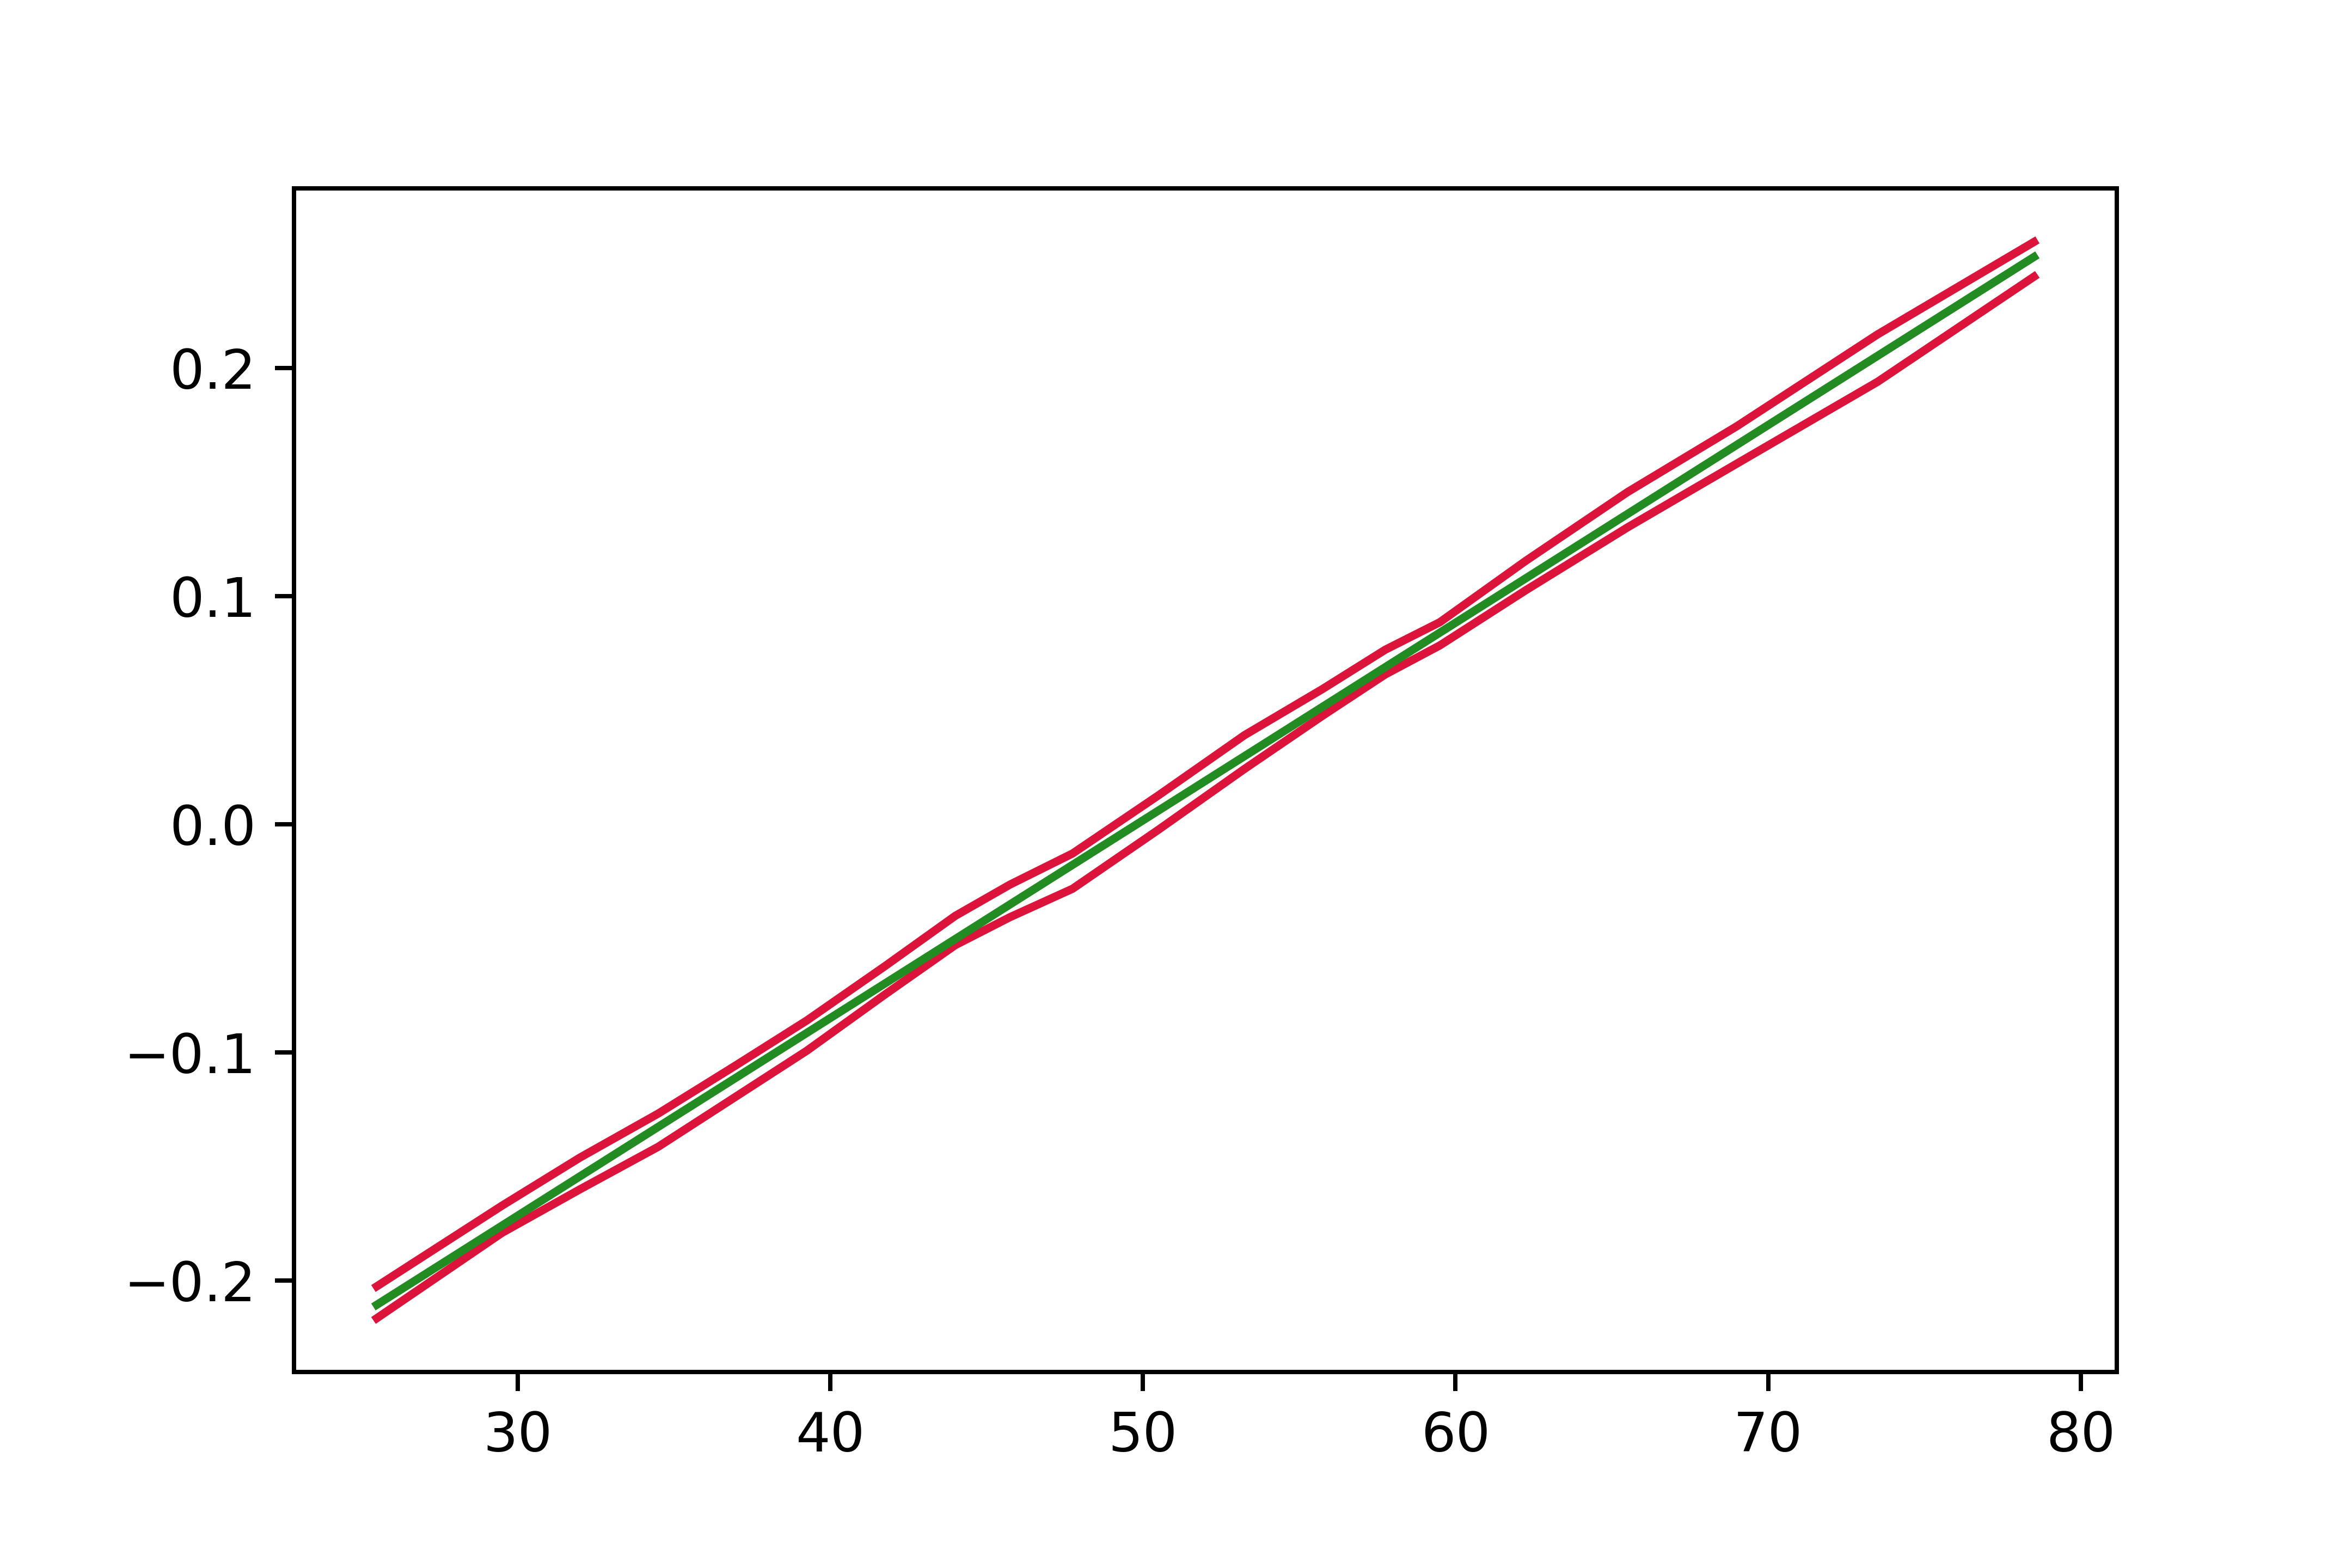
\includegraphics[width=\linewidth]{figures/ALE/chNDexp/spec2_linear_AGE.png}
        \caption{Spec 2 - linear}
    \end{subfigure}%
    \begin{subfigure}{0.5\linewidth}
        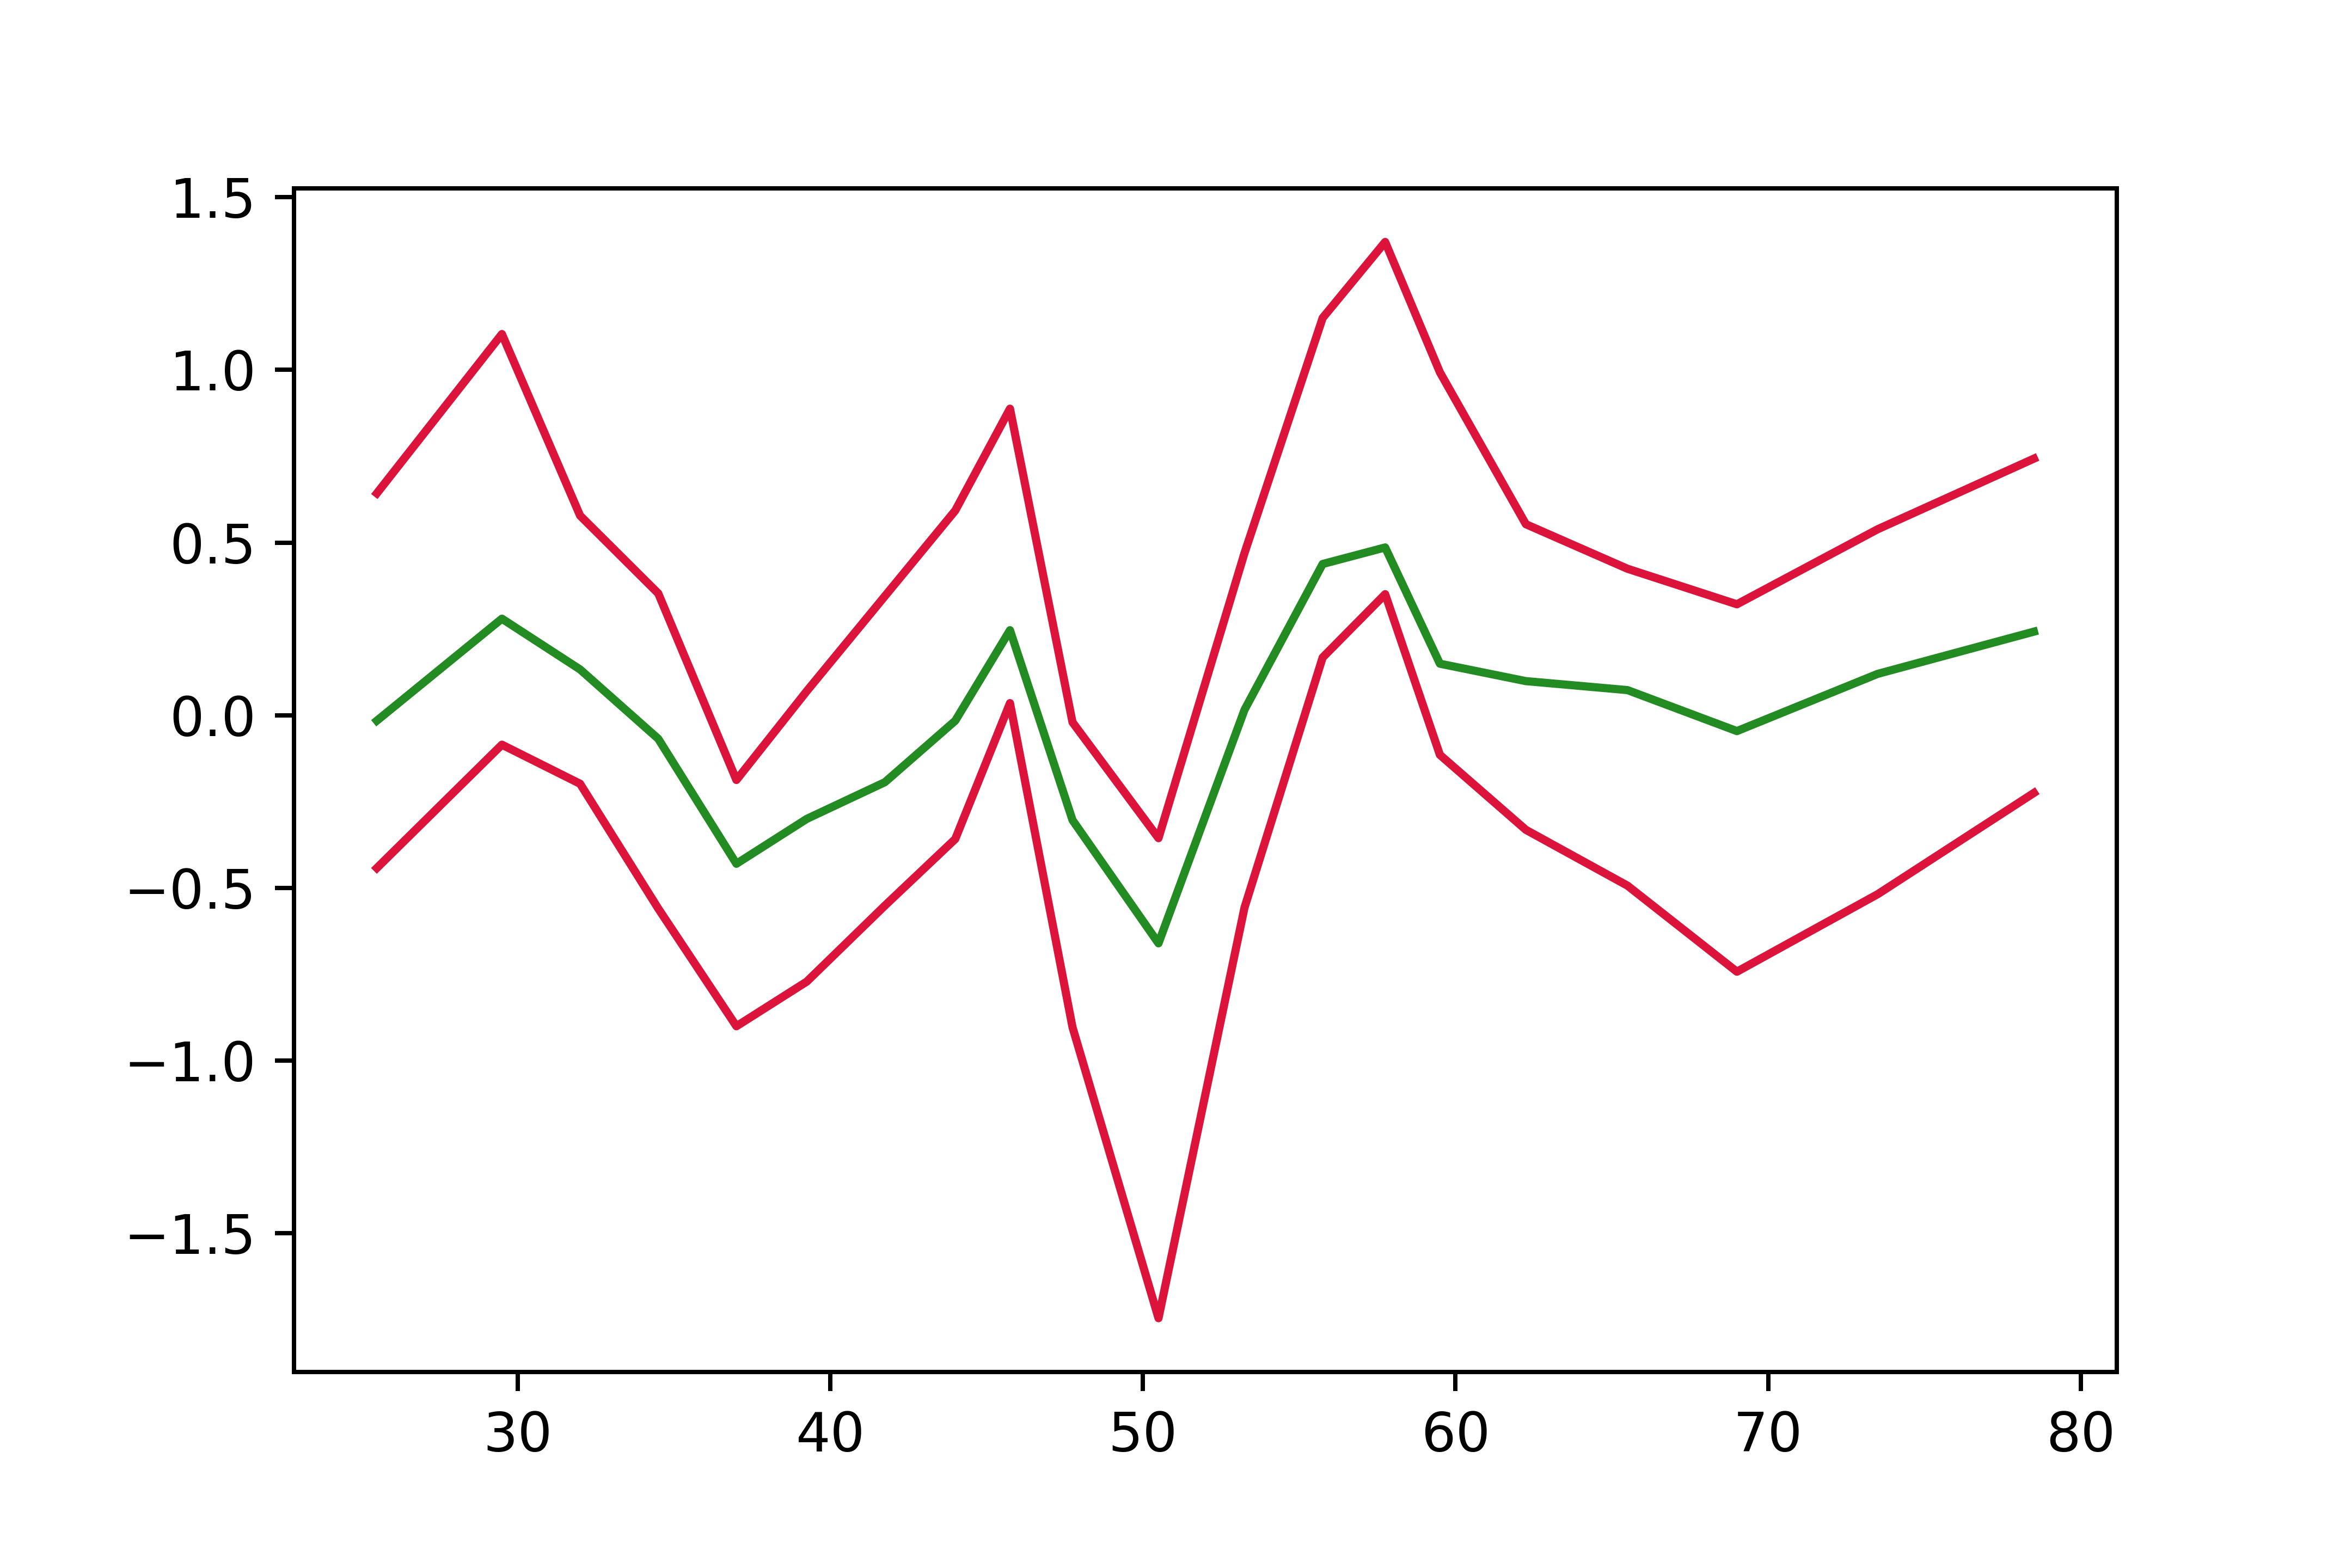
\includegraphics[width=\linewidth]{figures/ALE/chNDexp/spec2_cf_AGE.png}
        \caption{Spec 2 - causal forest }
    \end{subfigure}
    \caption{ALE of AGE in Specification 2 - non-durable expenditures}
    \label{app:ale_age_spec2}
\end{figure}

%!TOT - Age
\begin{figure}[h]
    \centering
    \begin{subfigure}{0.5\linewidth}
        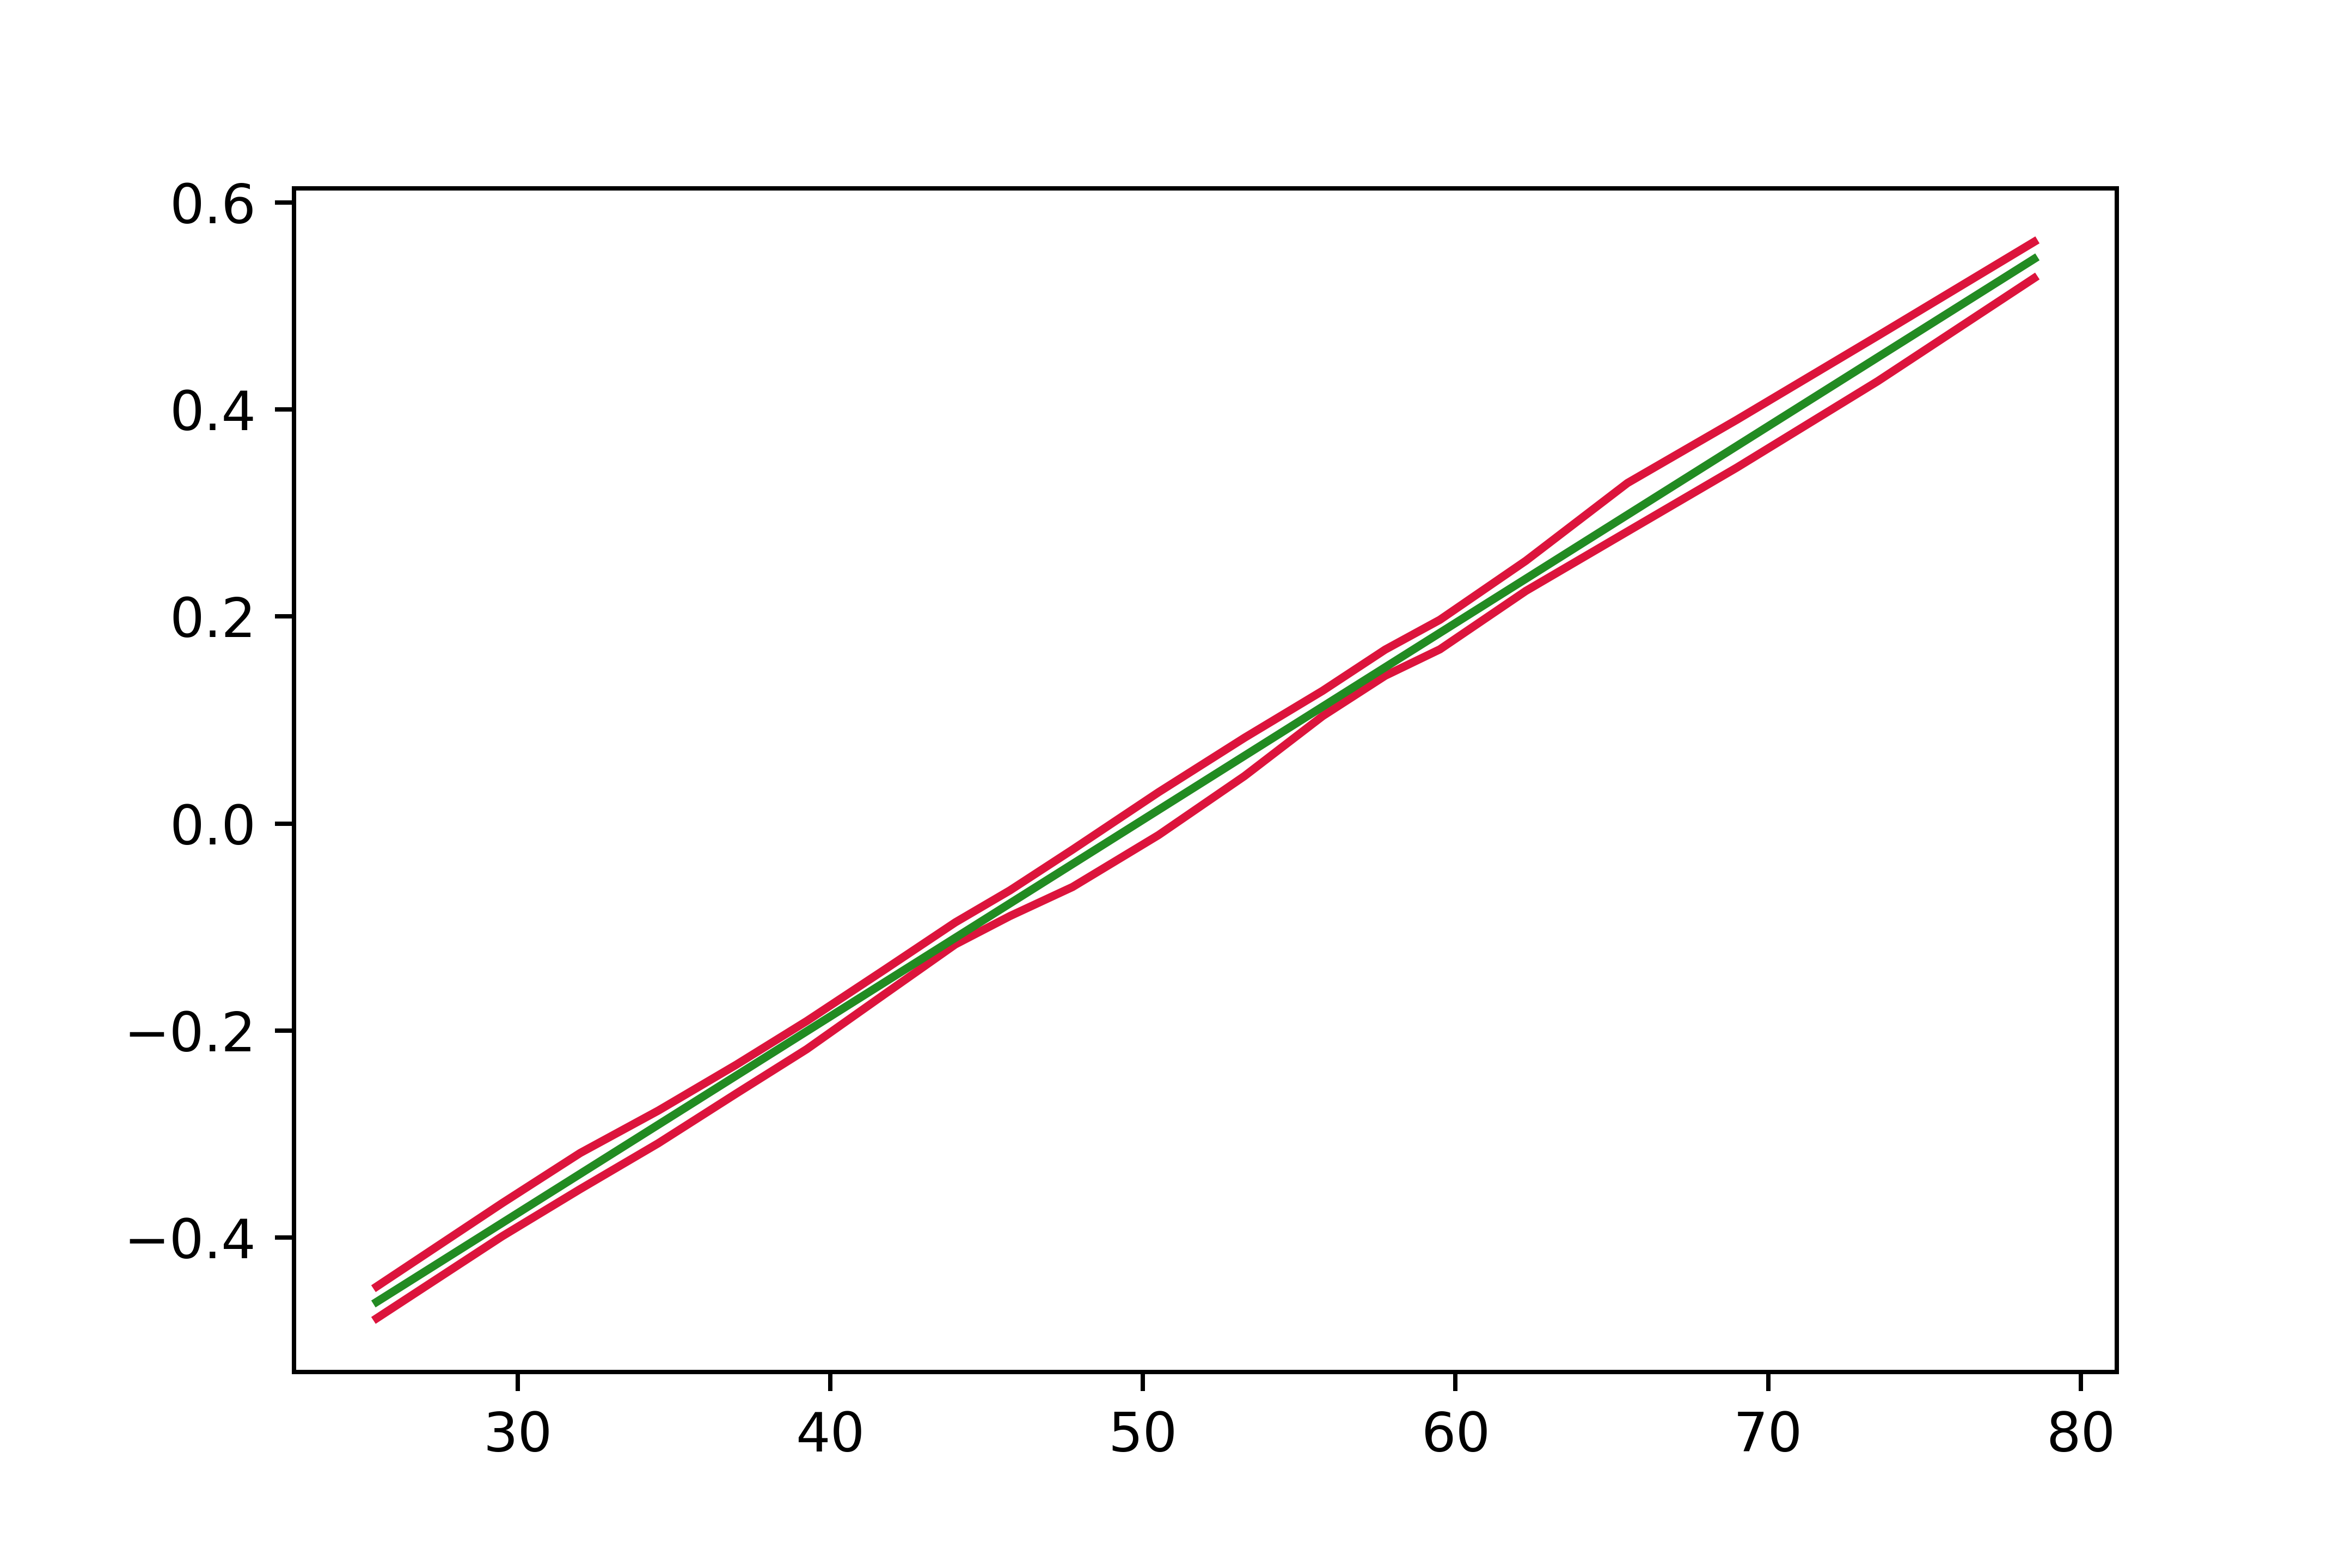
\includegraphics[width=\linewidth]{figures/ALE/chTOTexp/spec1_linear_AGE.png}
        \caption{Spec 1 - linear}
    \end{subfigure}%
    \begin{subfigure}{0.5\linewidth}
        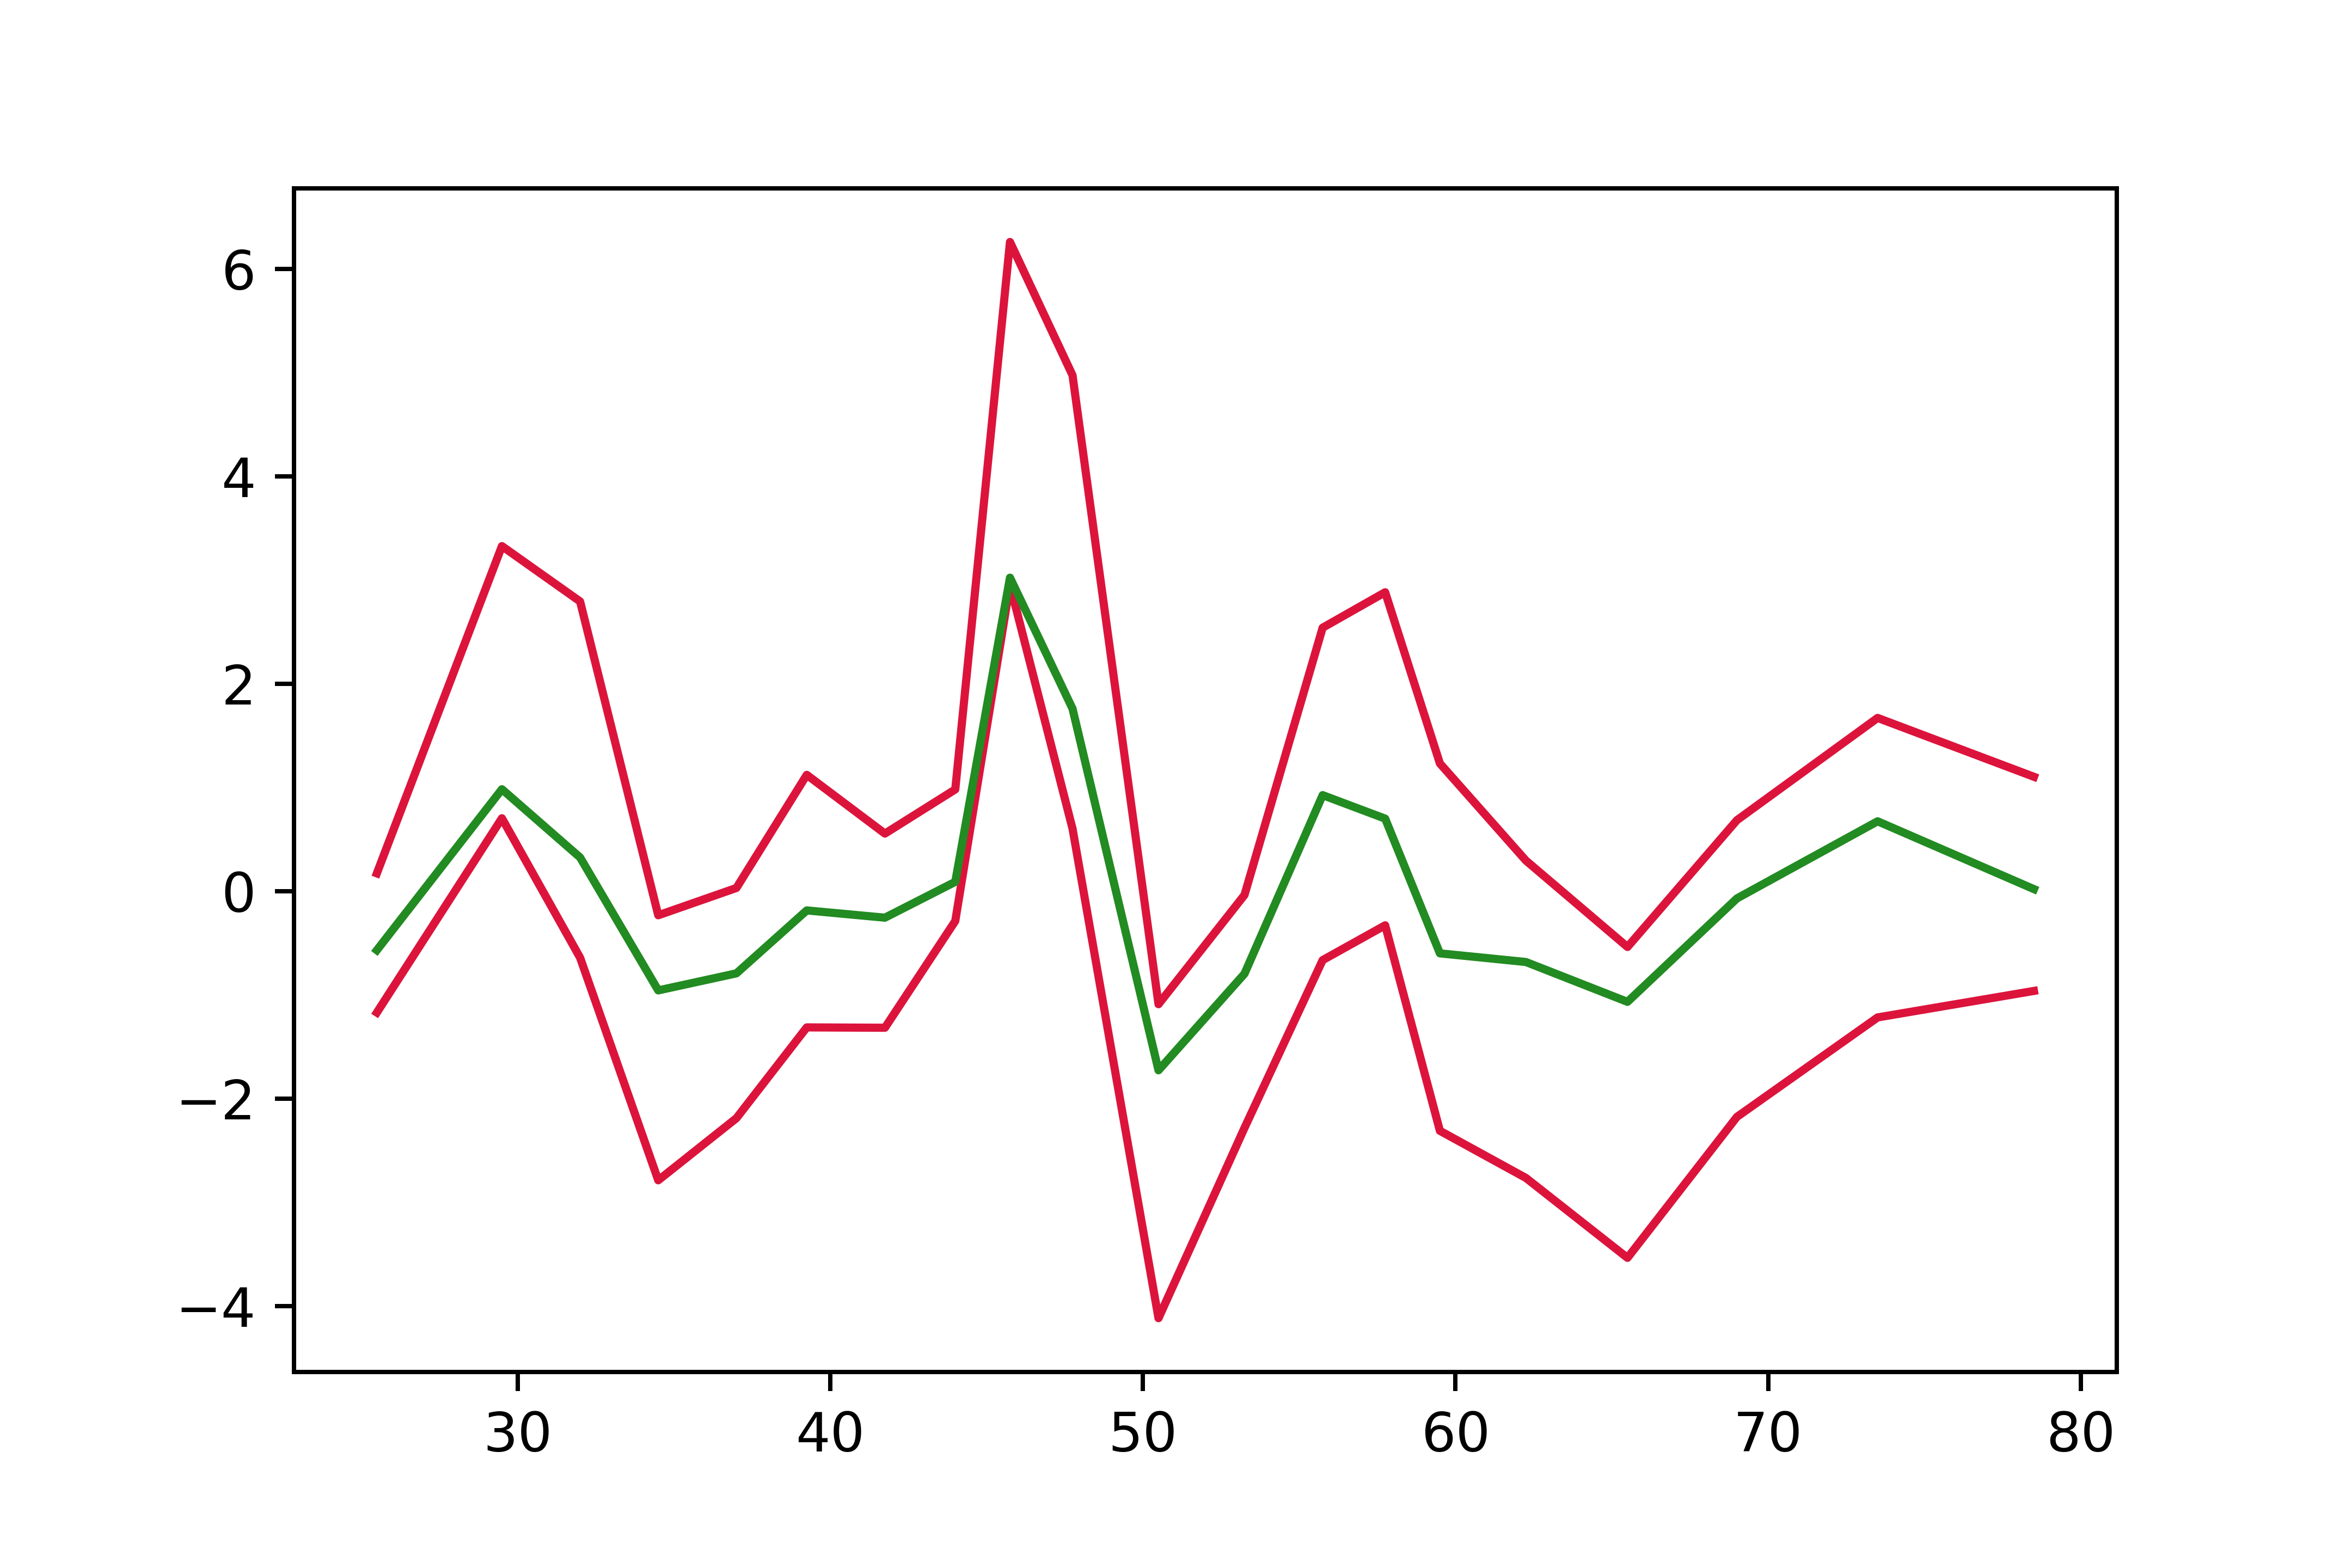
\includegraphics[width=\linewidth]{figures/ALE/chTOTexp/spec1_cf_AGE.png}
        \caption{Spec 1 - causal forest}
    \end{subfigure}

    \begin{subfigure}{0.5\linewidth}
        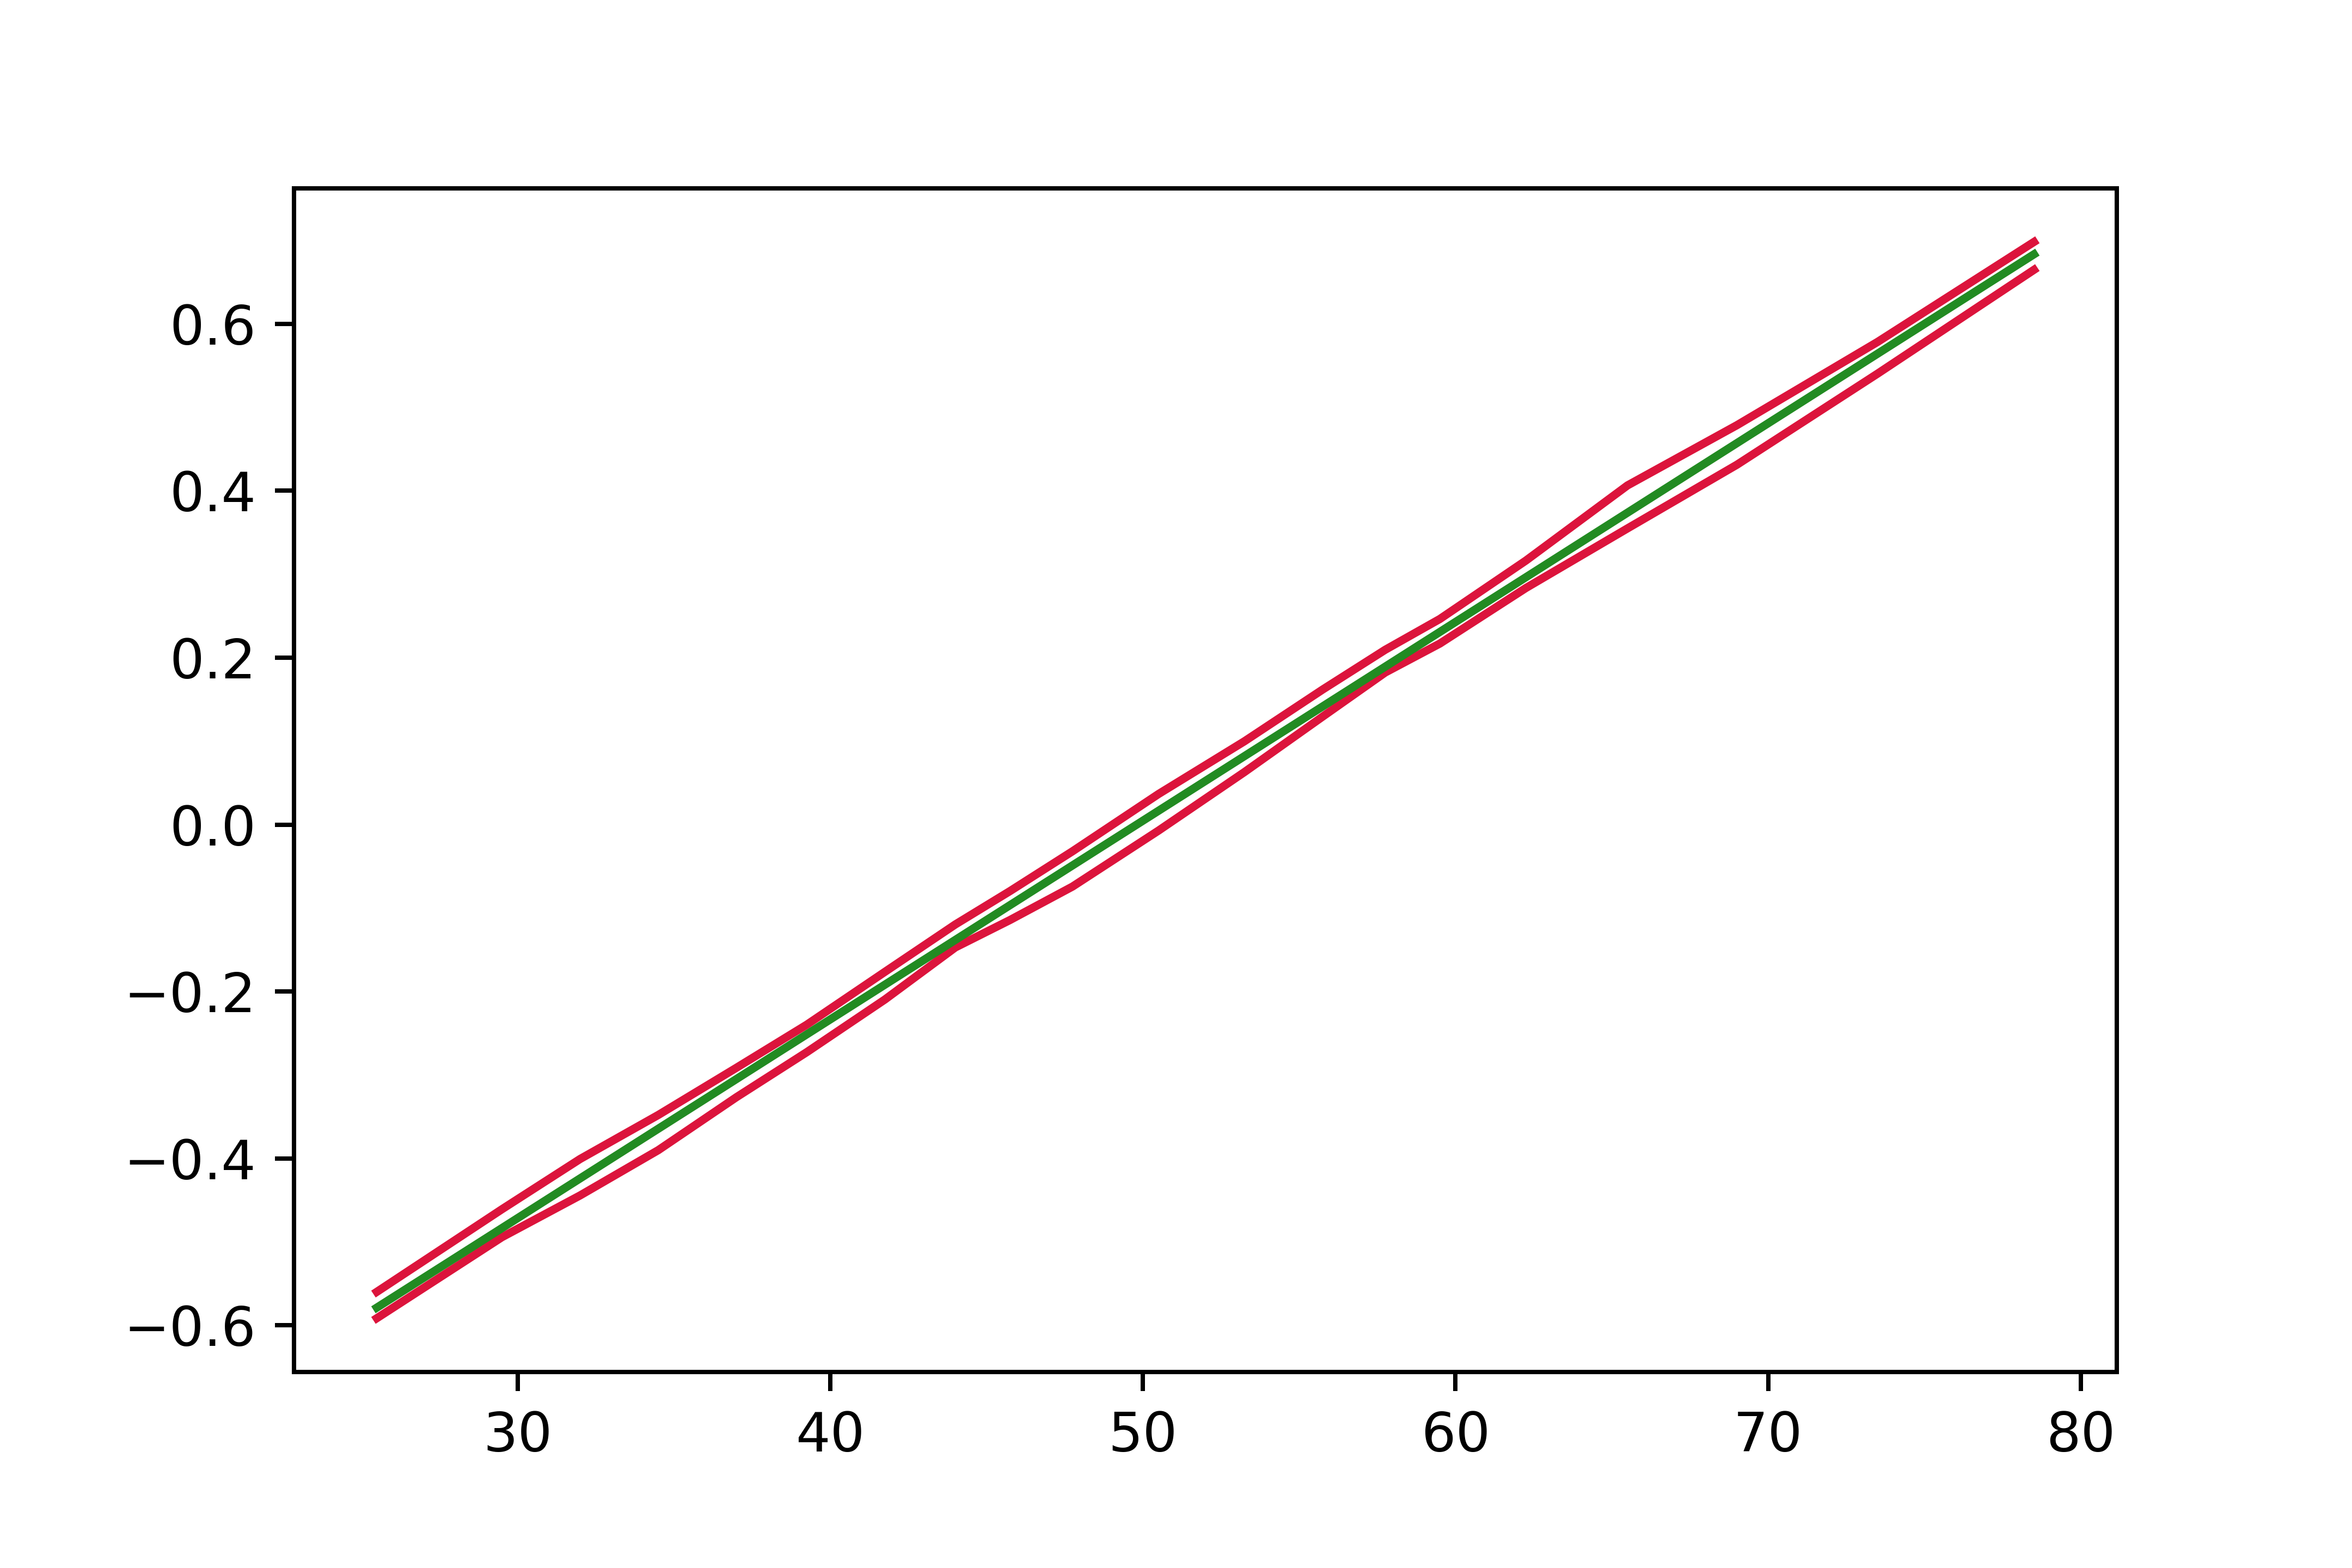
\includegraphics[width=\linewidth]{figures/ALE/chTOTexp/spec2_linear_AGE.png}
        \caption{Spec 2 - linear}
    \end{subfigure}%
    \begin{subfigure}{0.5\linewidth}
        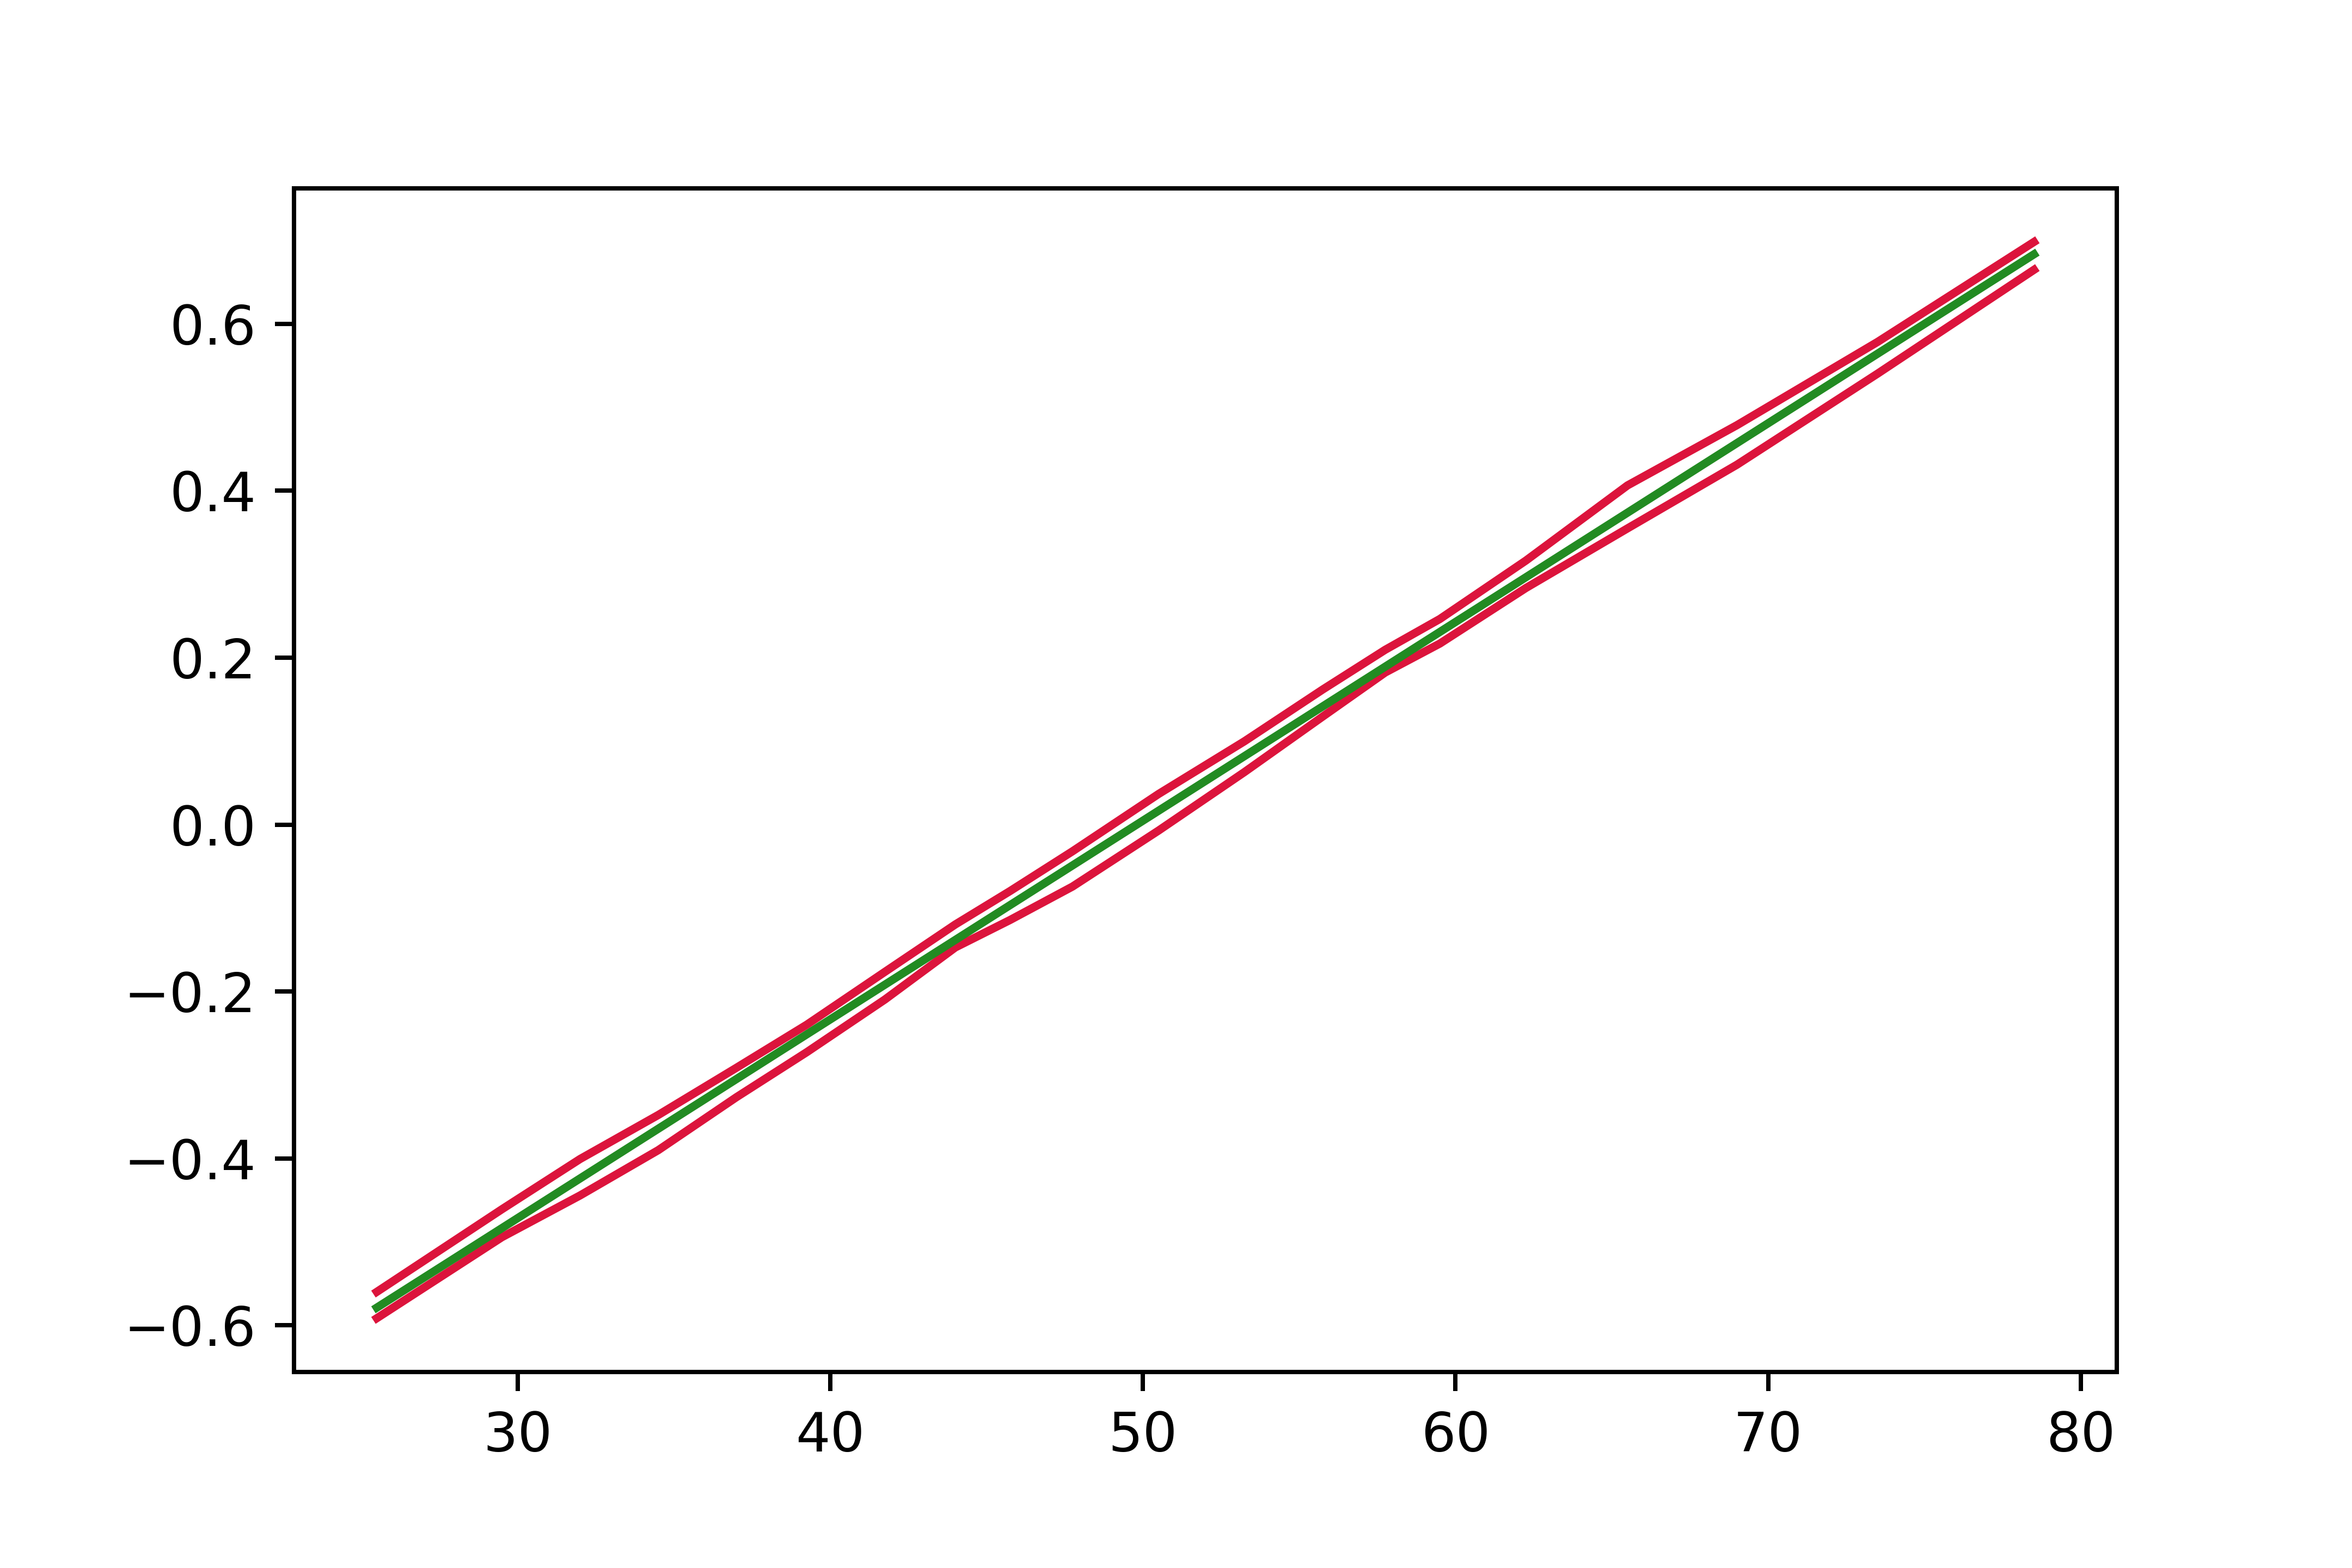
\includegraphics[width=\linewidth]{figures/ALE/chTOTexp/spec2_linear_AGE.png}
        \caption{Spec 2 - causal forest}
    \end{subfigure}

    \begin{subfigure}{0.5\linewidth}
        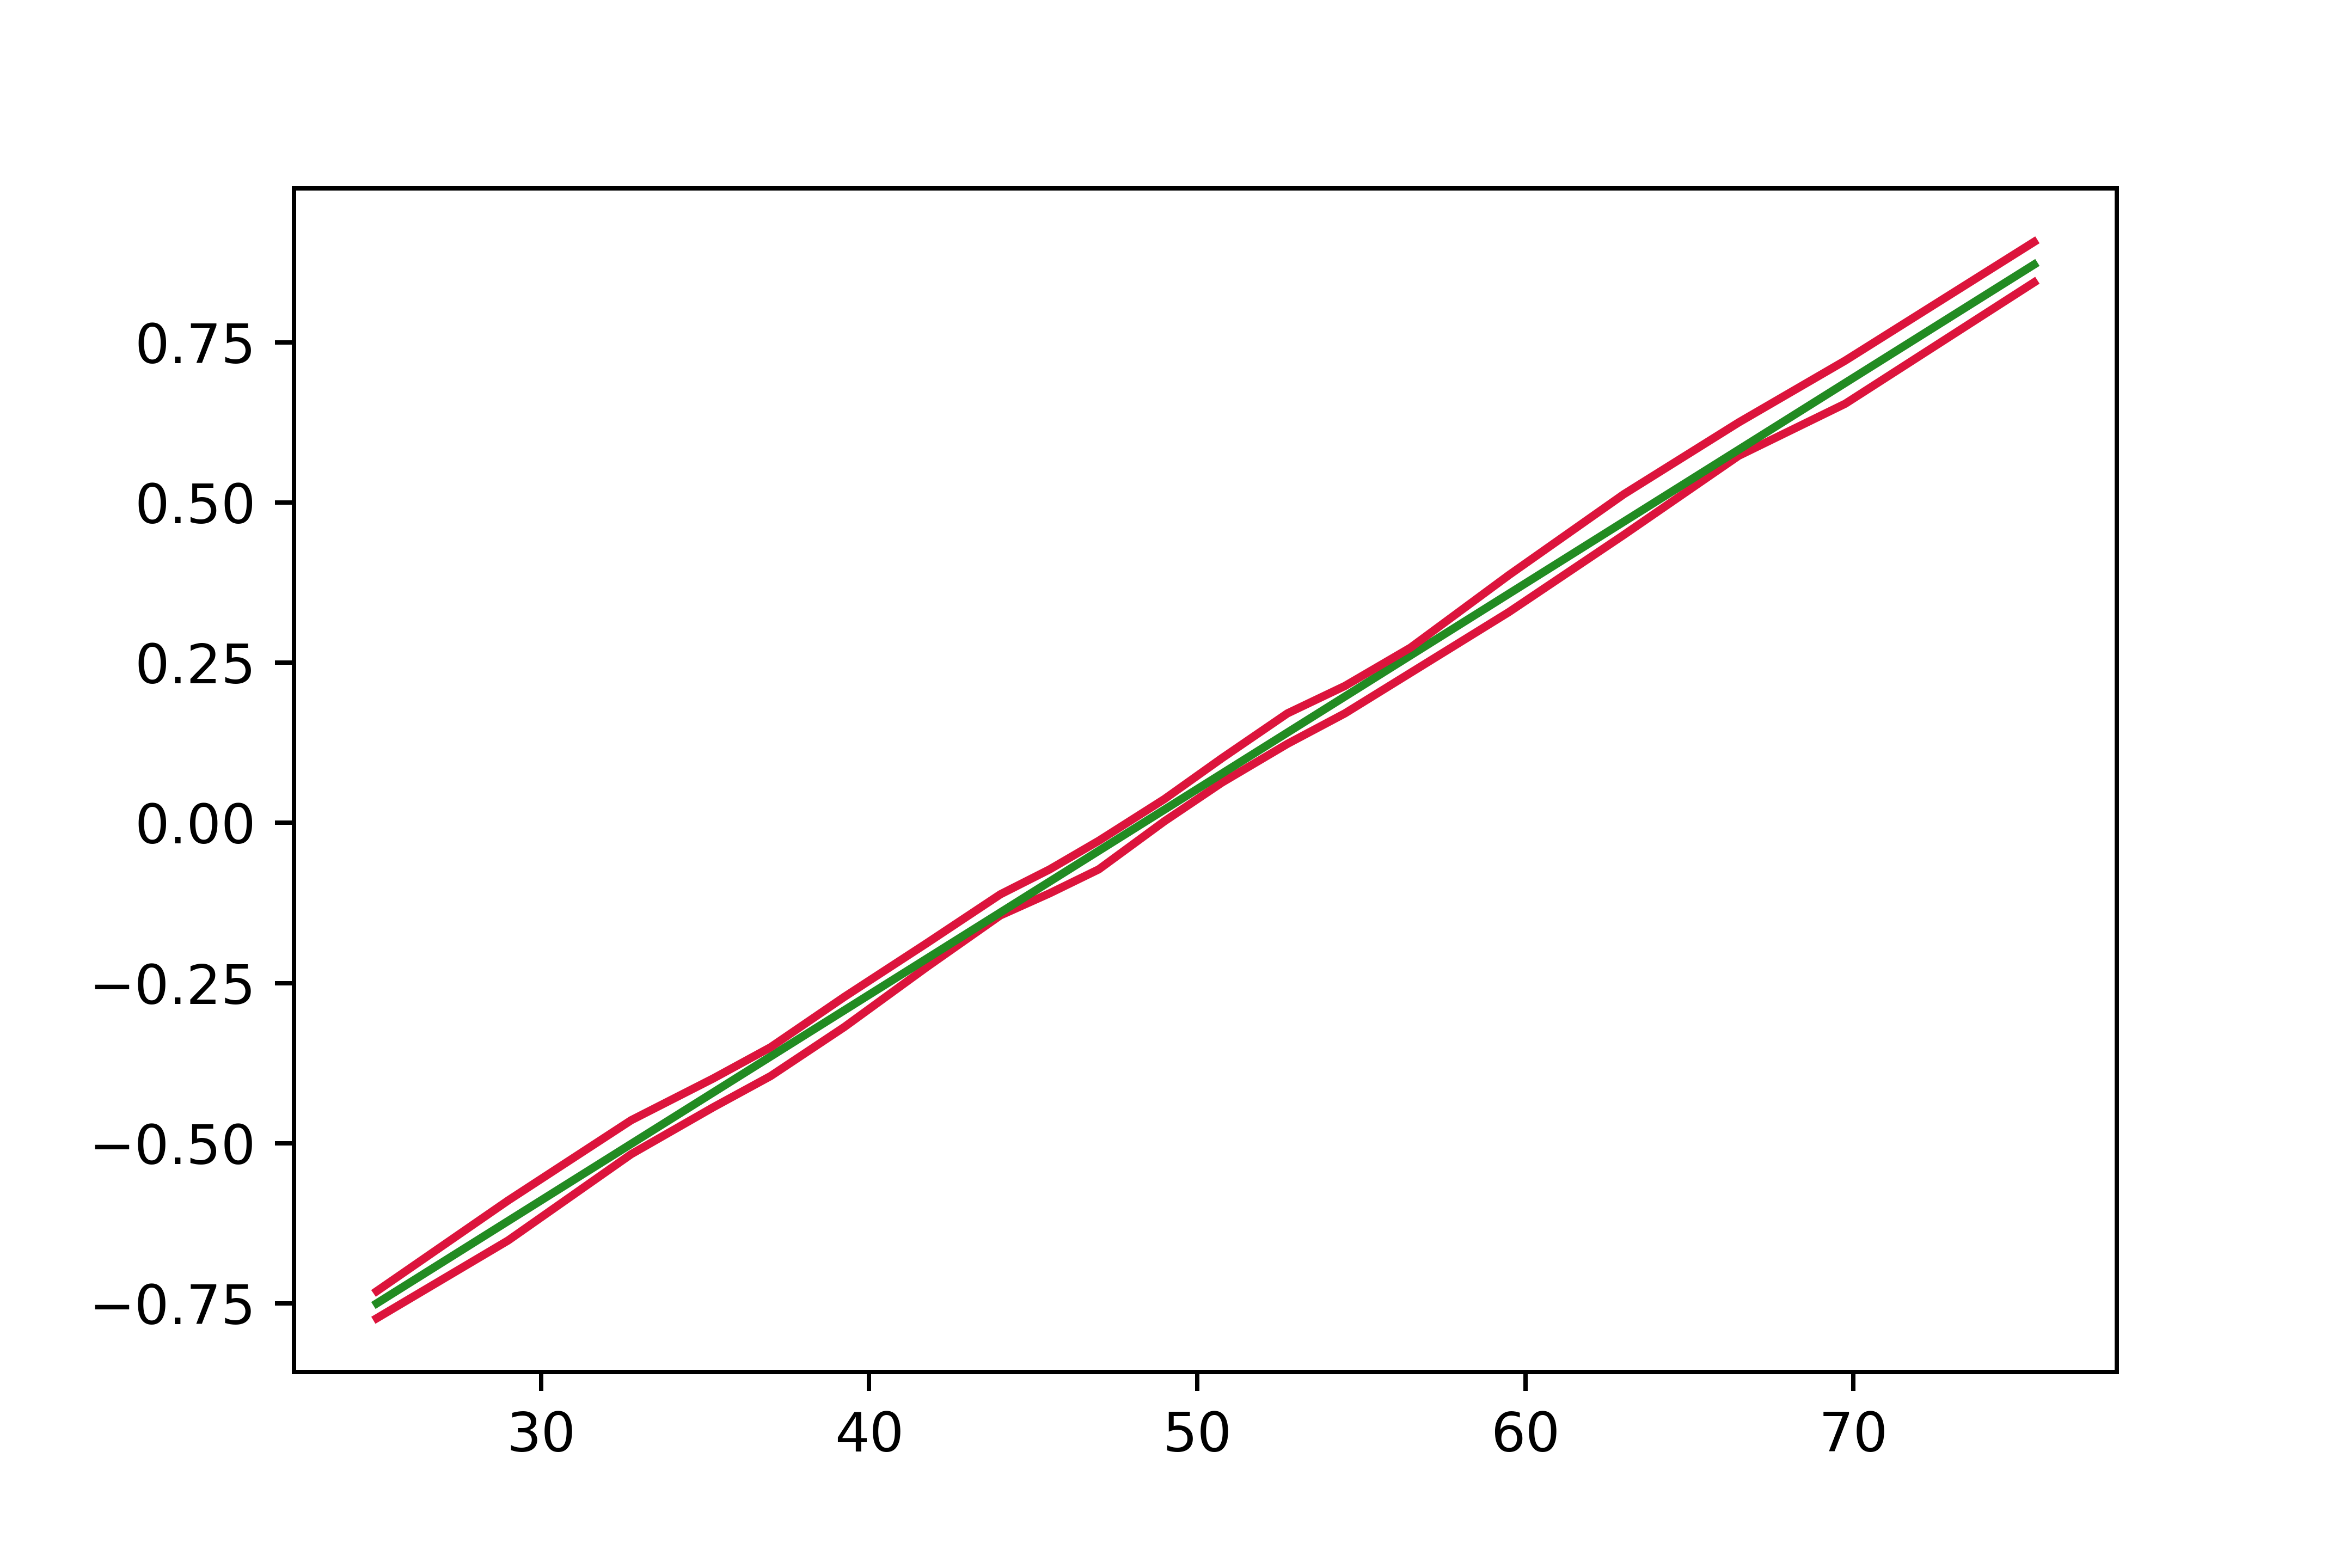
\includegraphics[width=\linewidth]{figures/ALE/chTOTexp/spec3_linear_AGE.png}
        \caption{Spec 3 - linear}
    \end{subfigure}%
    \begin{subfigure}{0.5\linewidth}
        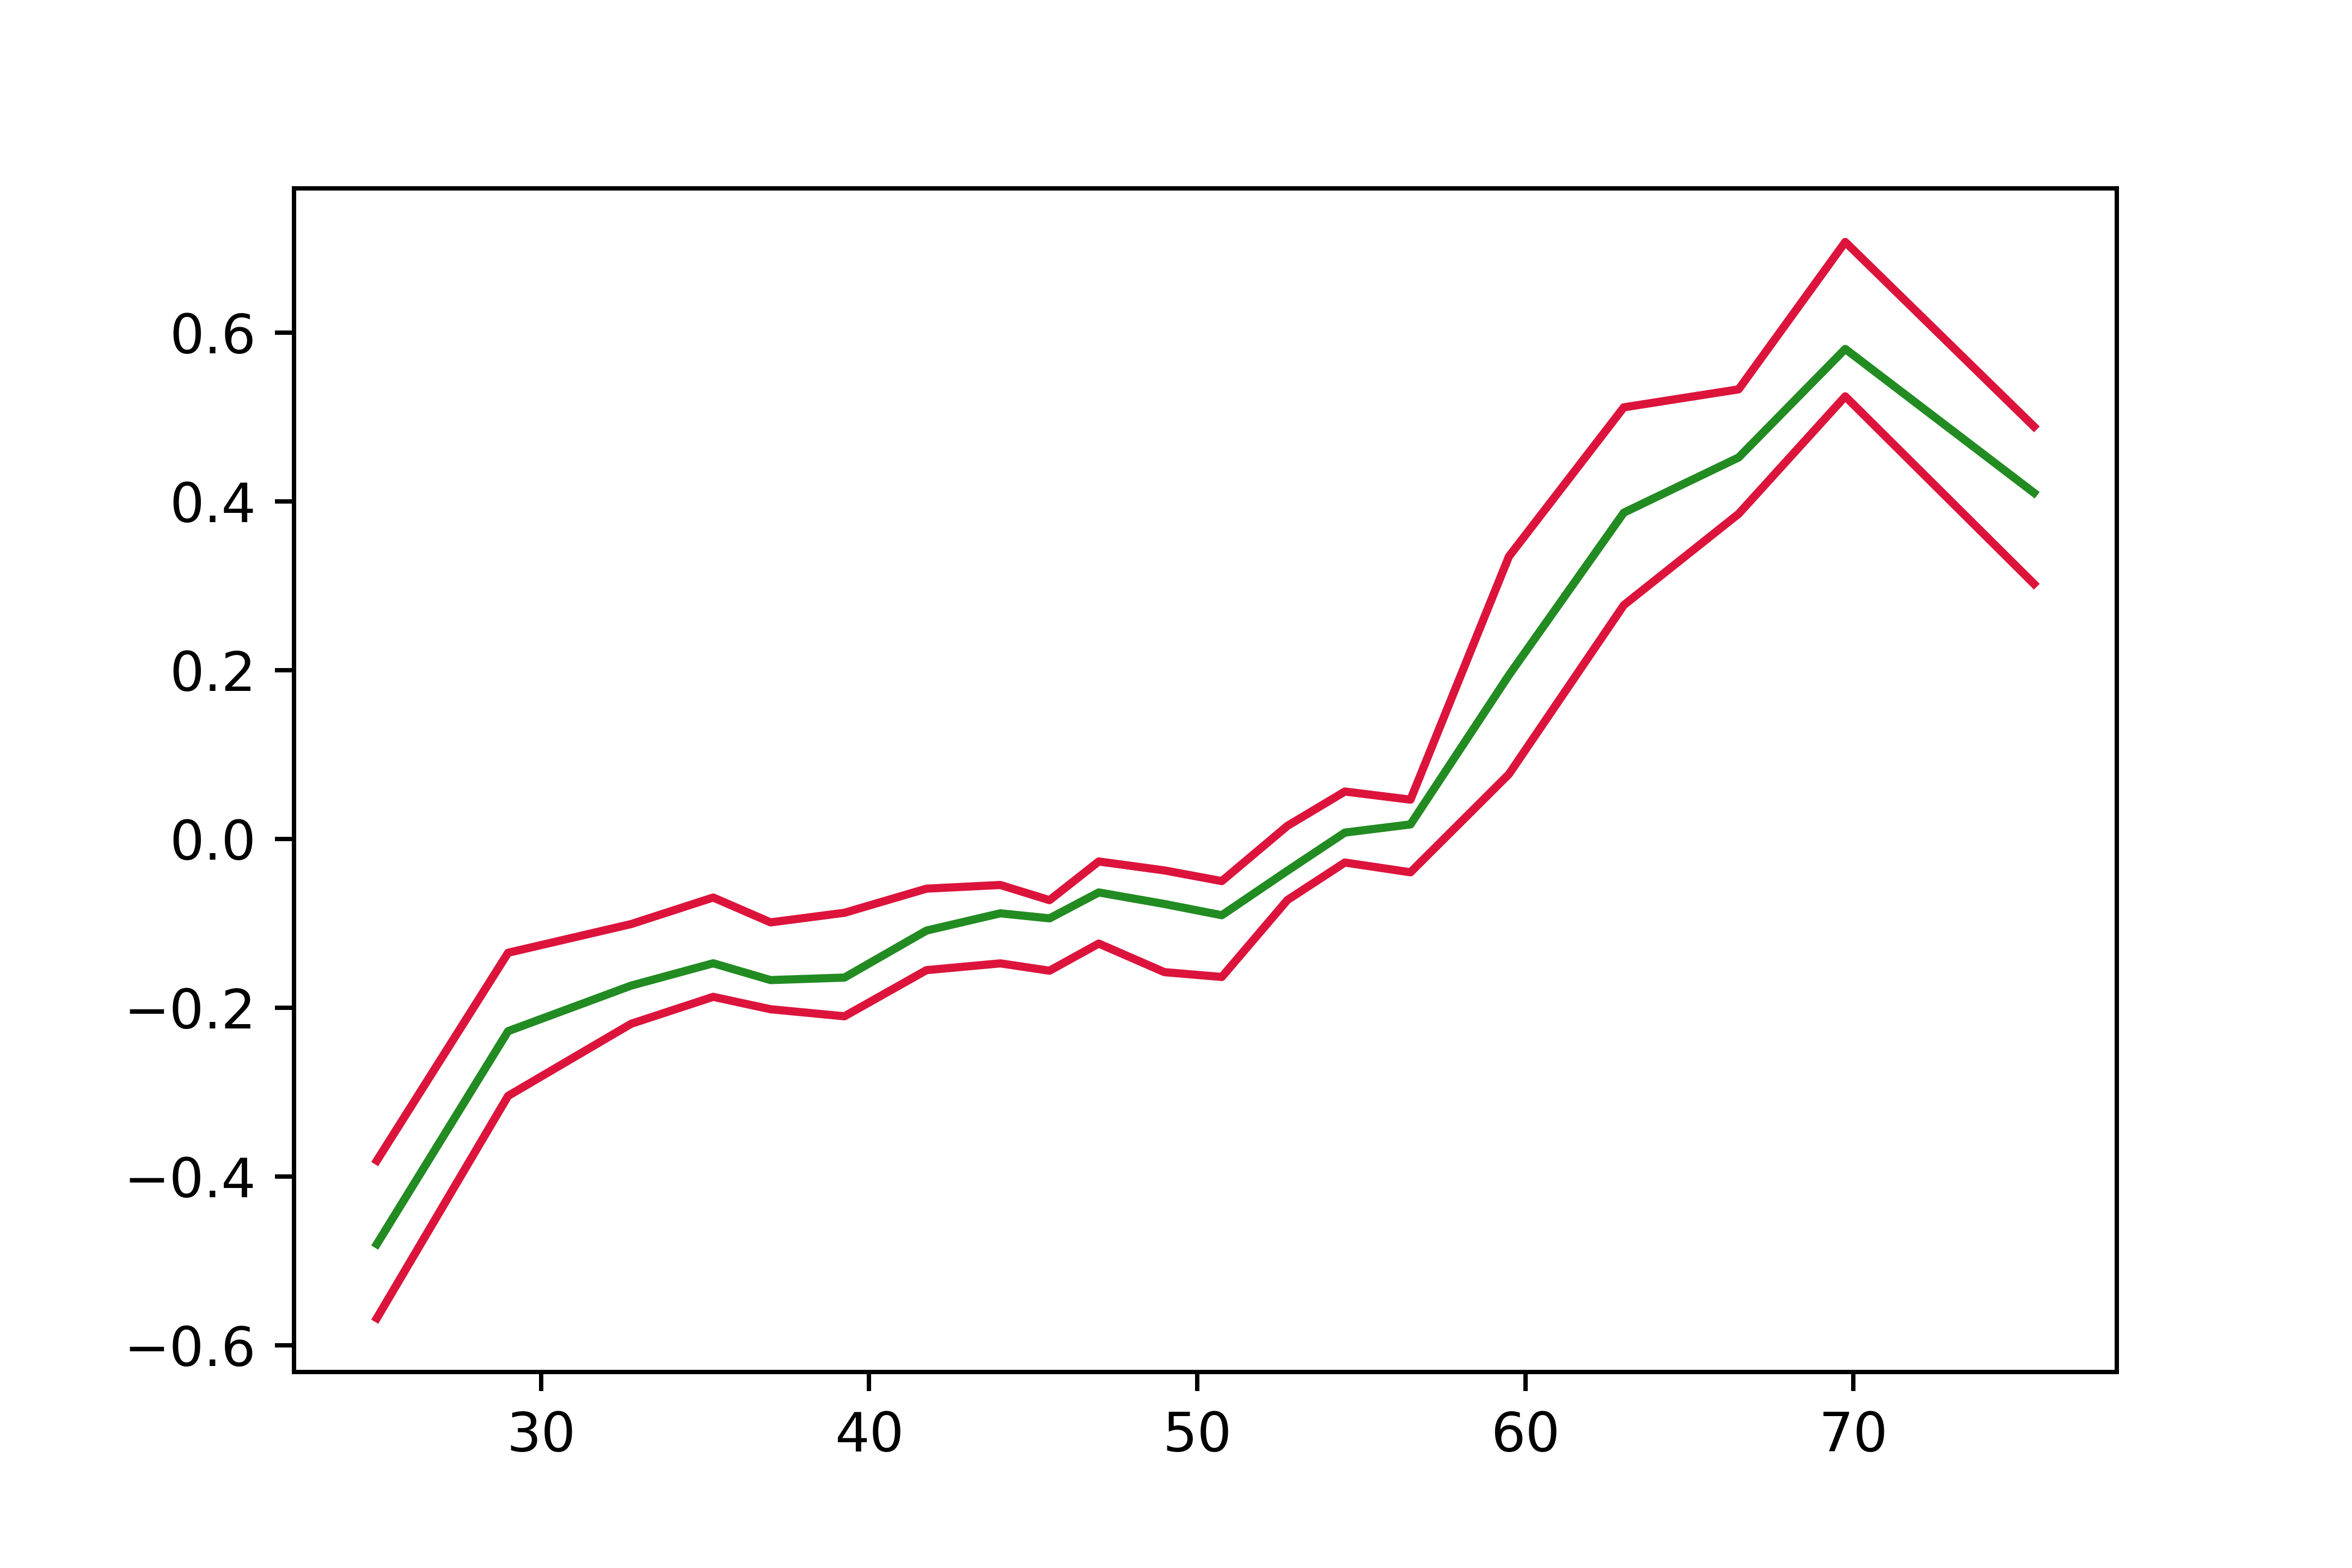
\includegraphics[width=\linewidth]{figures/ALE/chTOTexp/spec3_cf_AGE.png}
        \caption{Spec 3 - causal forest}
    \end{subfigure}
    \caption{ALE of AGE - total expenditures}
    \label{app:ale_age_tot}
\end{figure}

%!TOT - Fin Stat
\begin{figure}[h]
    \centering
    \begin{subfigure}{0.5\linewidth}
        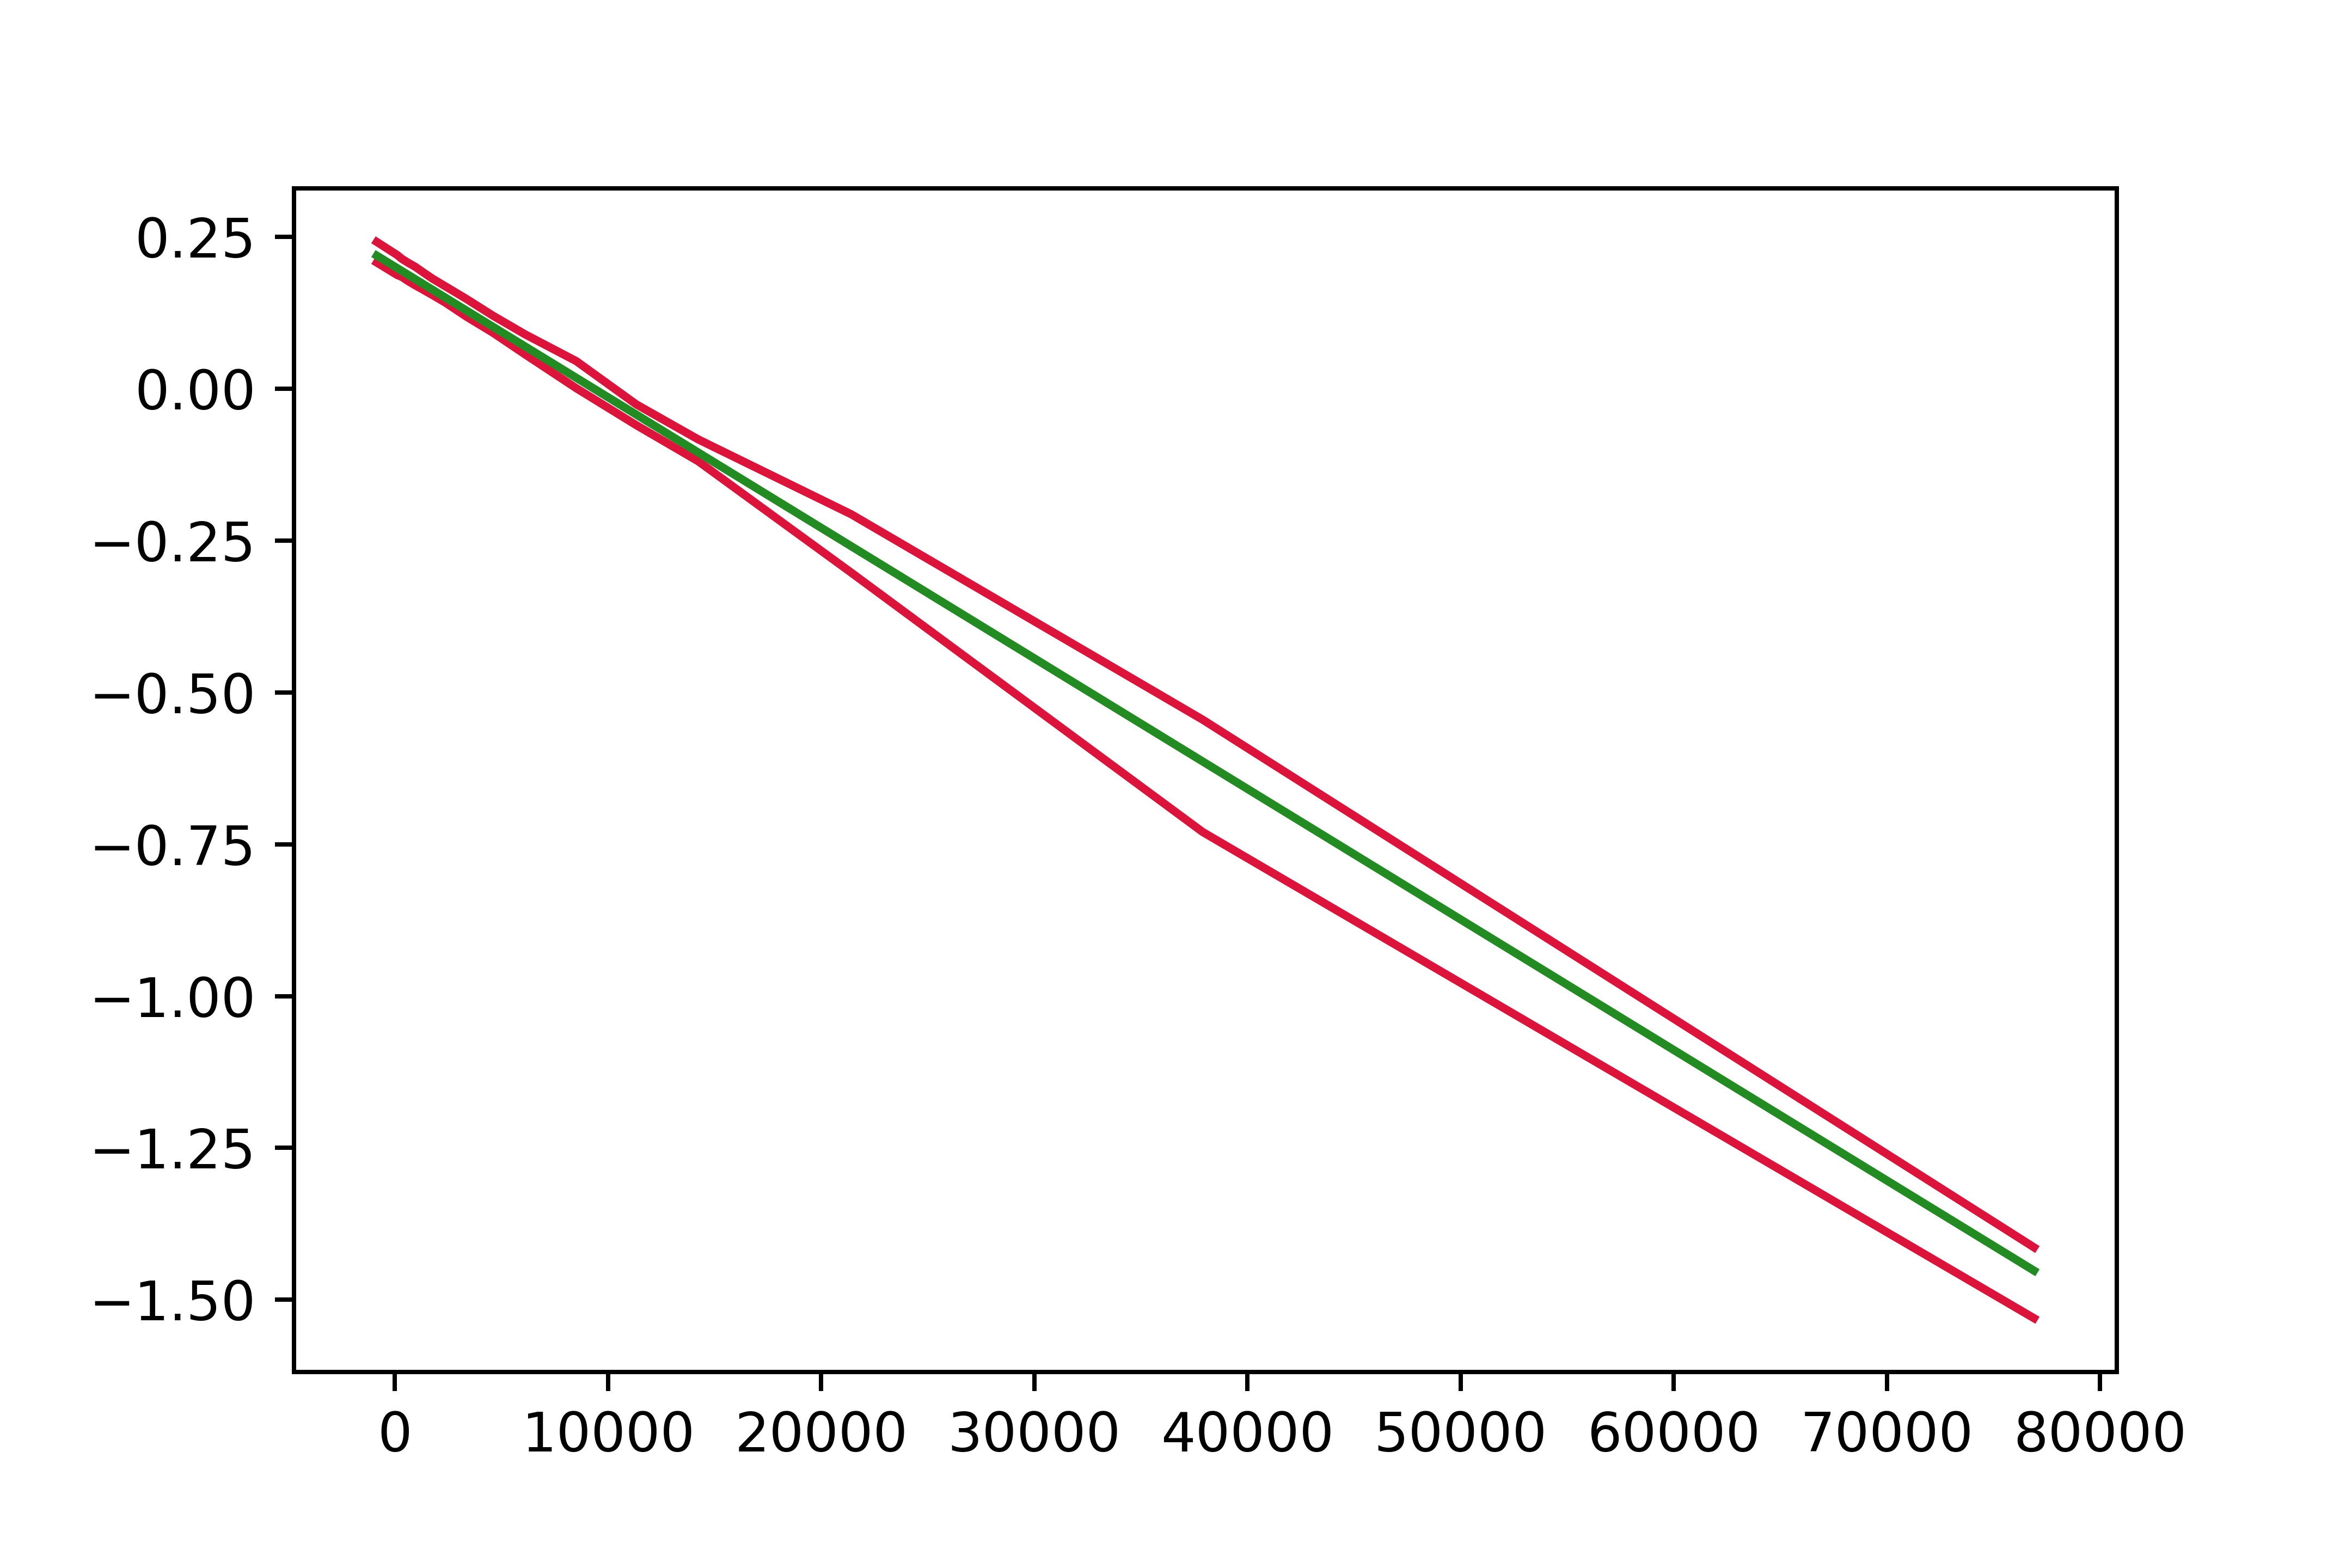
\includegraphics[width=\linewidth]{figures/ALE/chTOTexp/spec3_linear_liqassii.png}
        \caption{Liquid Assets - linear}
    \end{subfigure}%
    \begin{subfigure}{0.5\linewidth}
        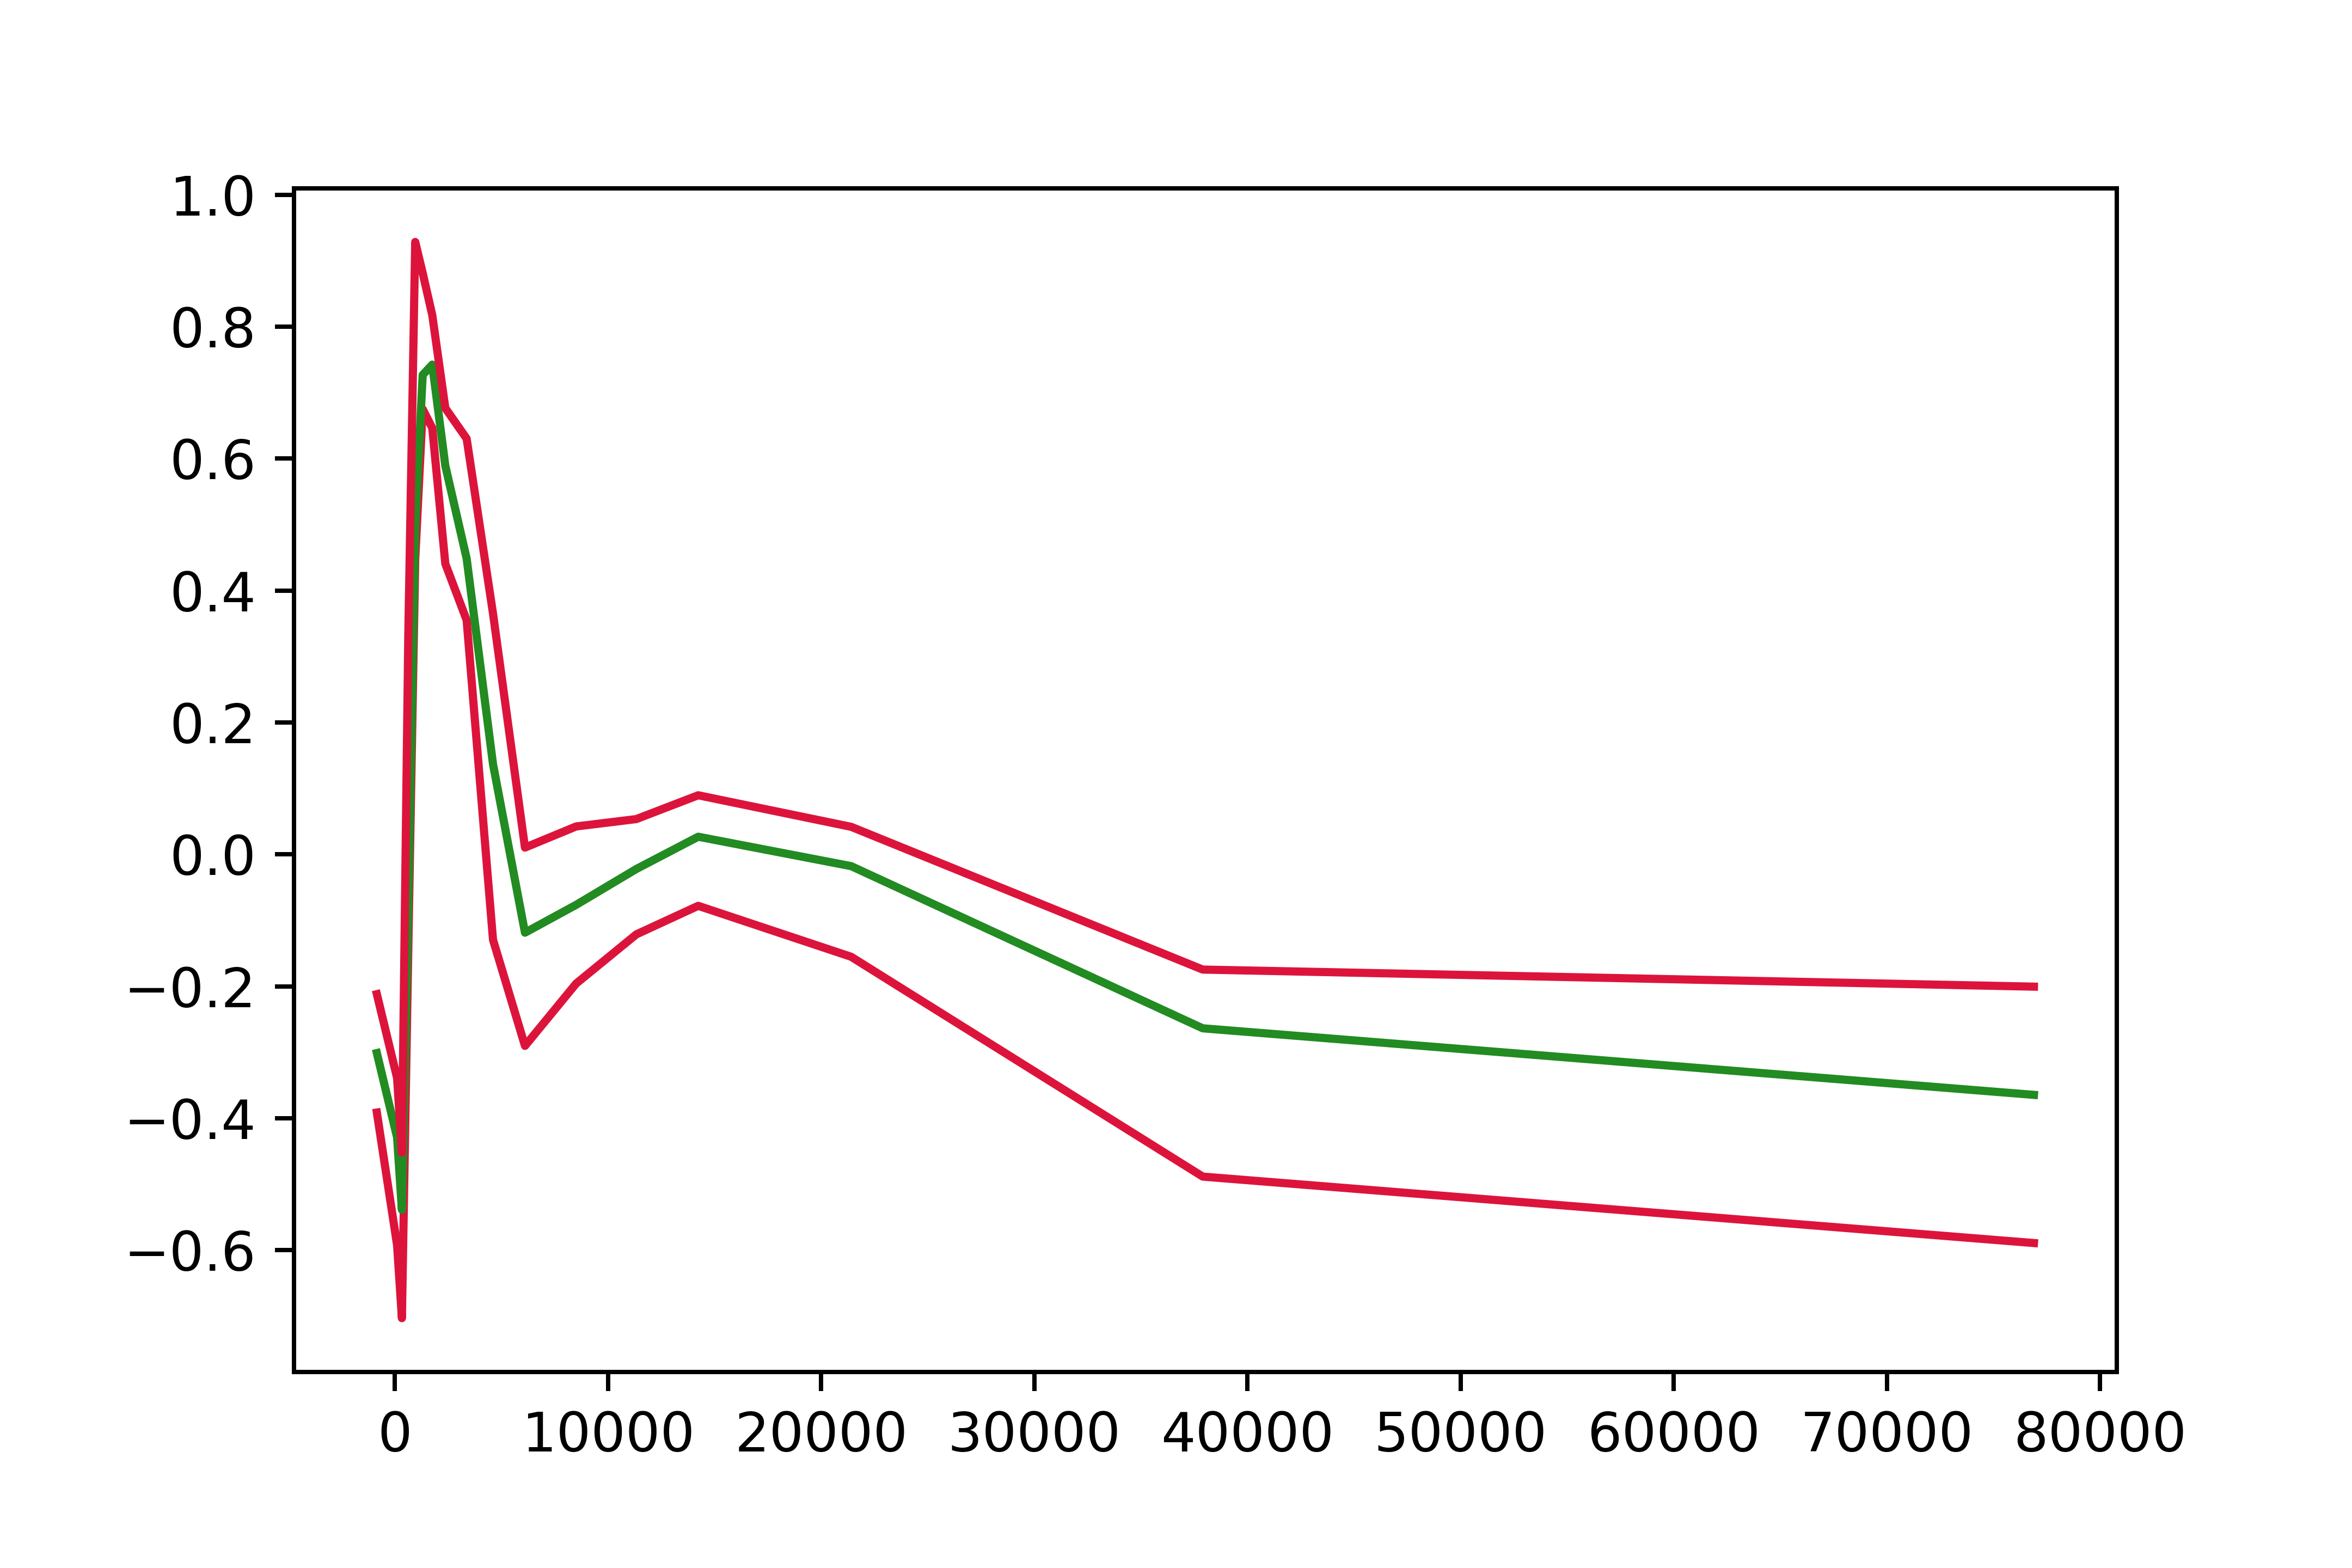
\includegraphics[width=\linewidth]{figures/ALE/chTOTexp/spec3_cf_liqassii.png}
        \caption{Liquid Assets - causal forest}
    \end{subfigure}

    \begin{subfigure}{0.5\linewidth}
        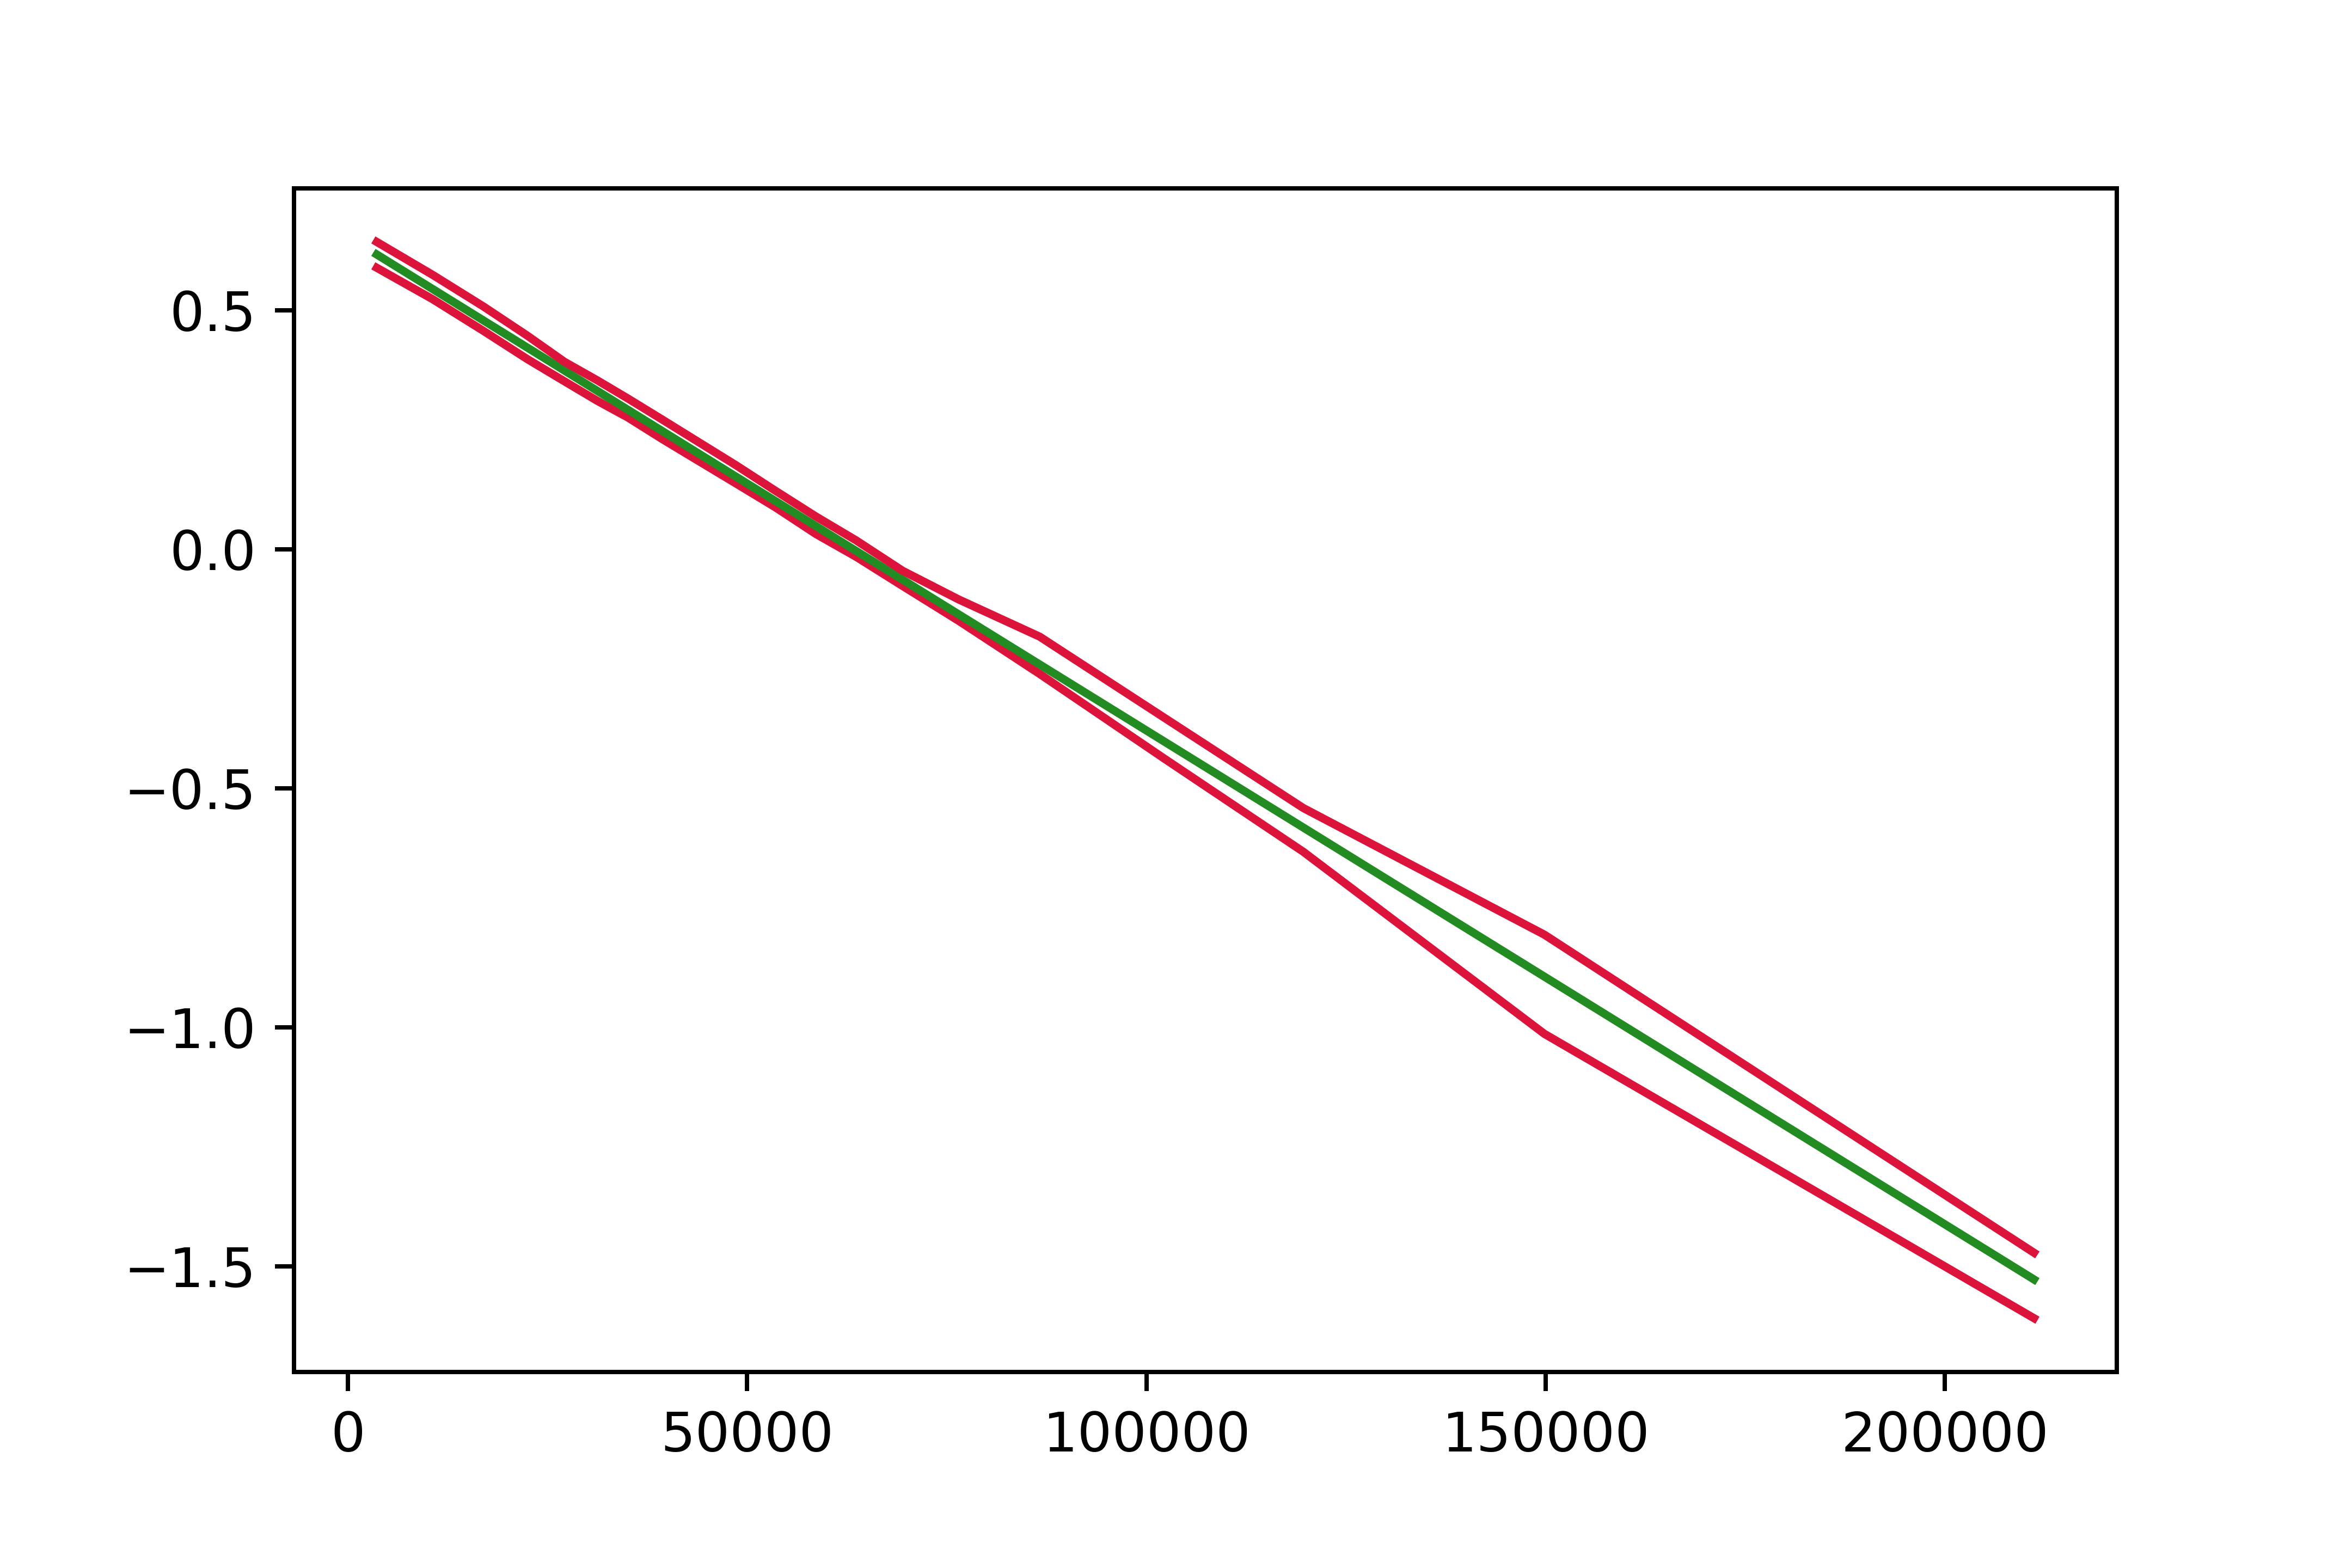
\includegraphics[width=\linewidth]{figures/ALE/chTOTexp/spec3_linear_FSALARYM.png}
        \caption{Salary - linear}
    \end{subfigure}%
    \begin{subfigure}{0.5\linewidth}
        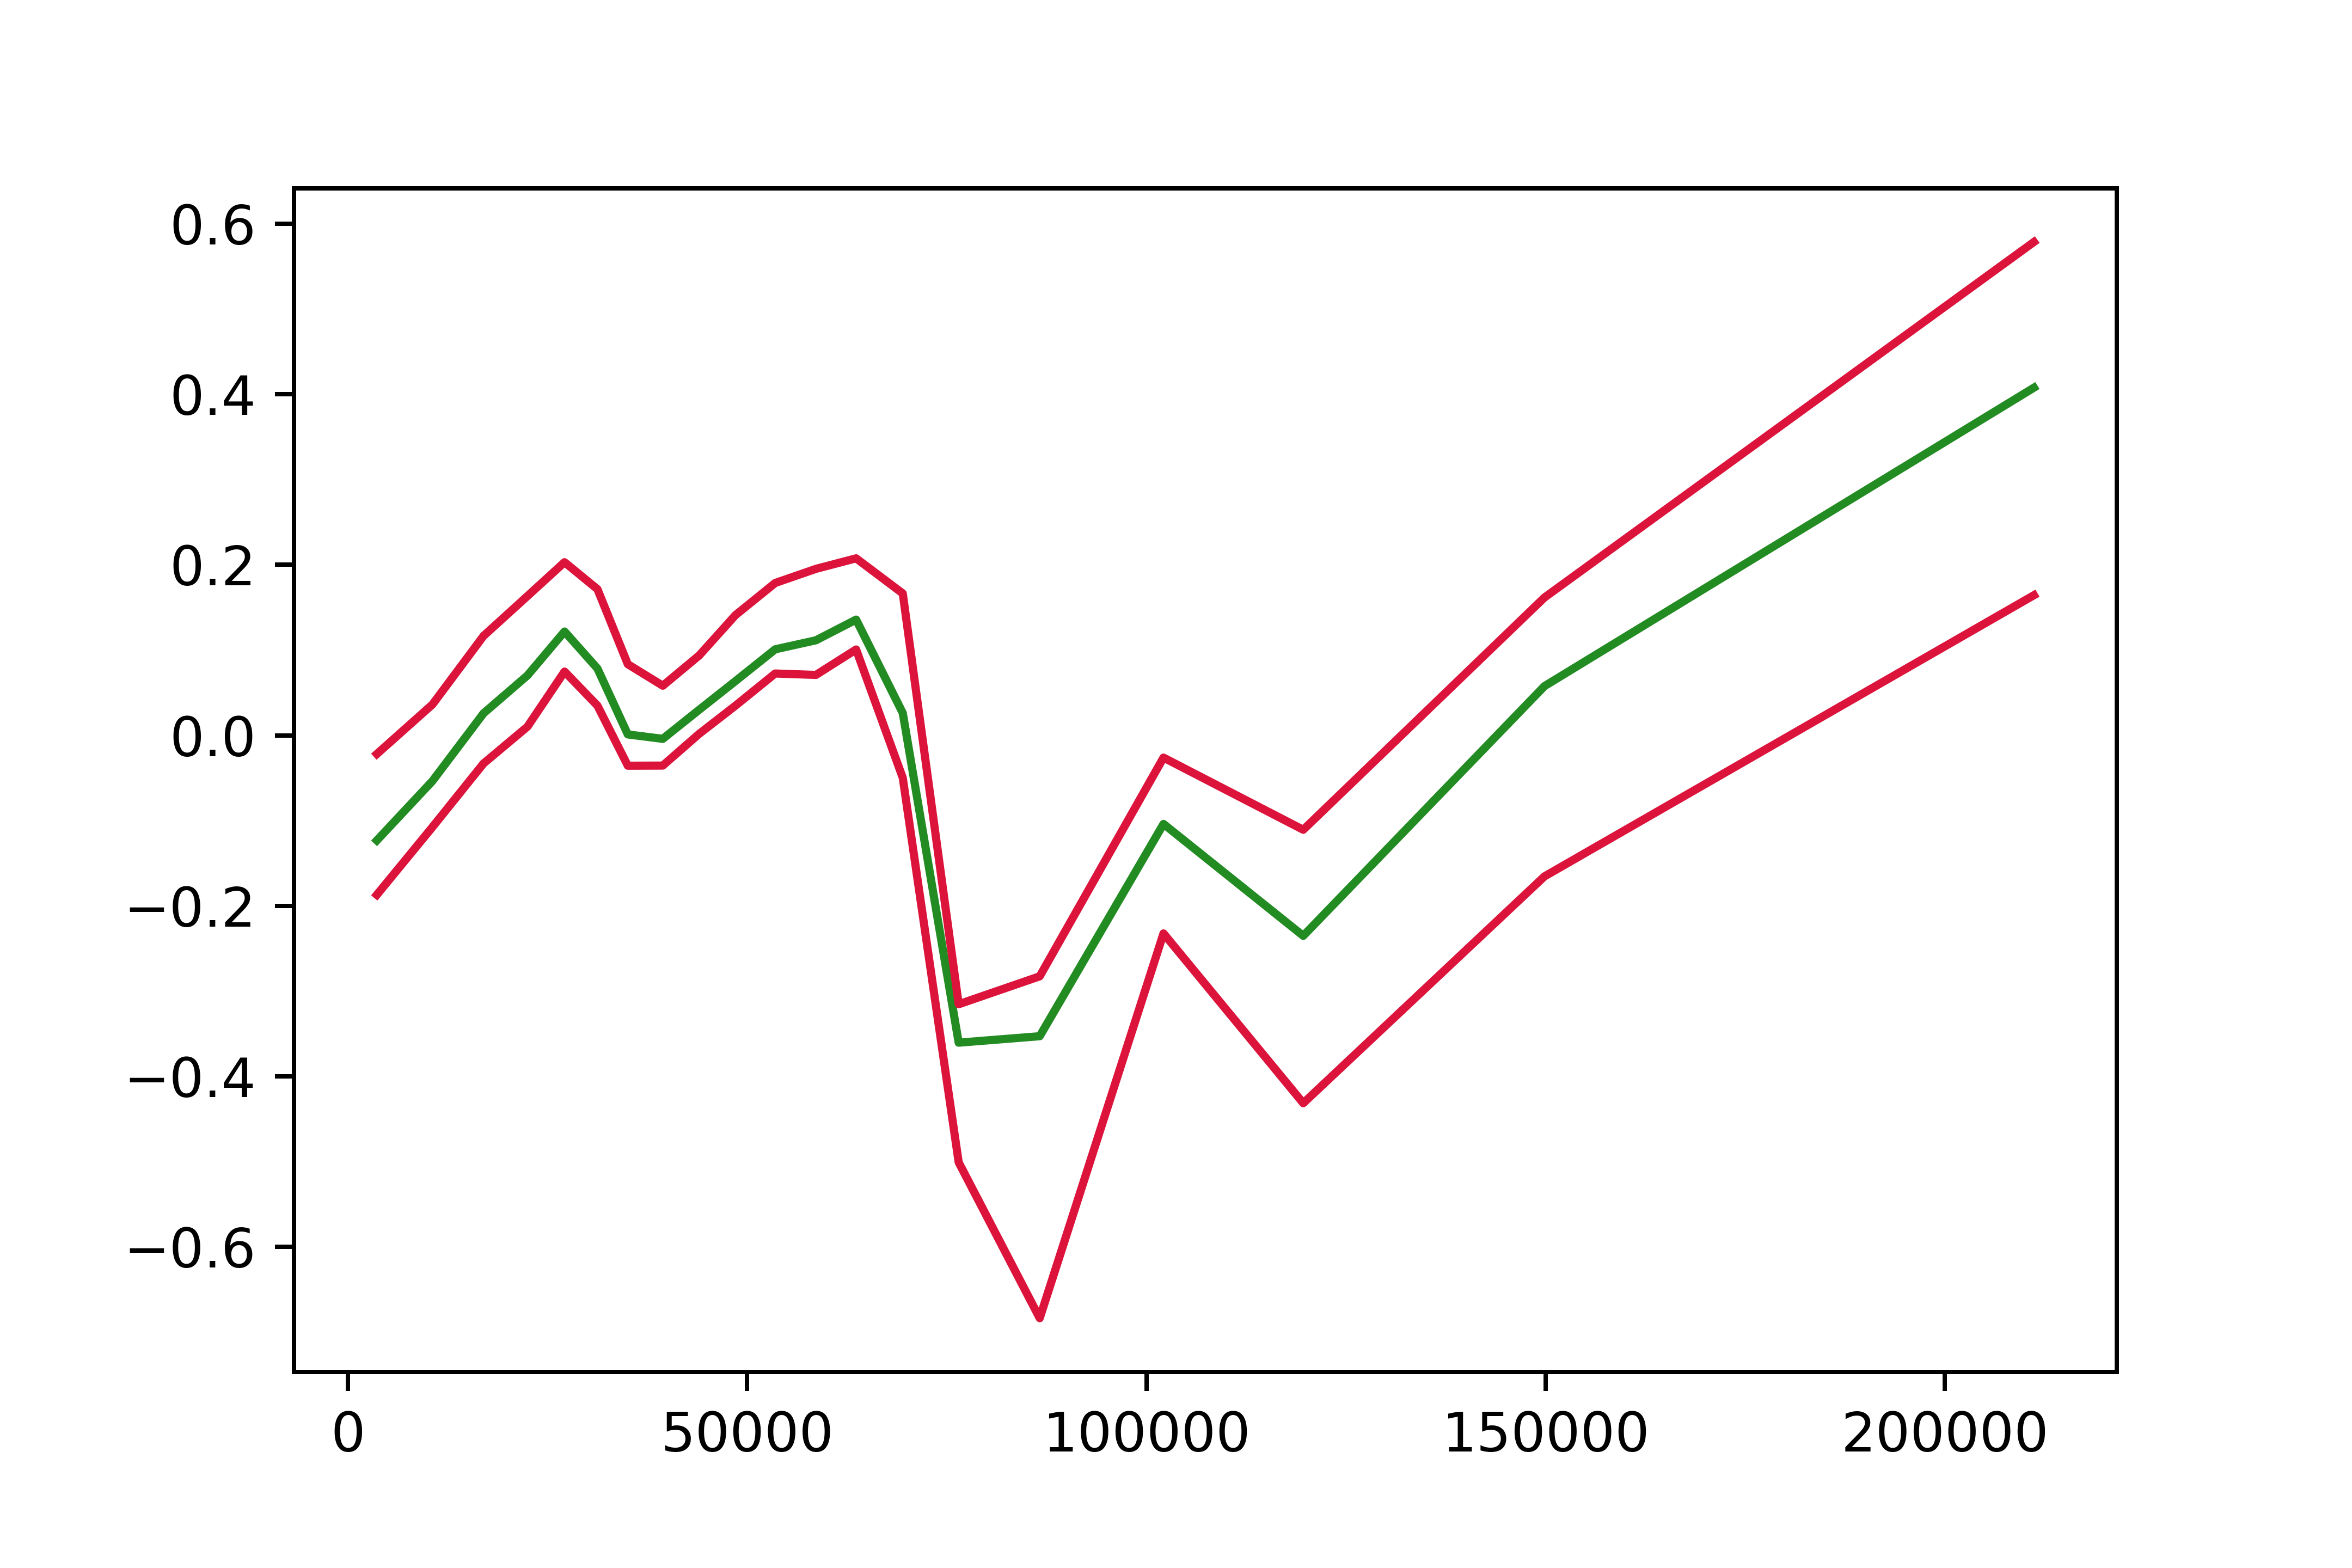
\includegraphics[width=\linewidth]{figures/ALE/chTOTexp/spec3_cf_FSALARYM.png}
        \caption{Salary - causal forest}
    \end{subfigure}

    \begin{subfigure}{0.5\linewidth}
        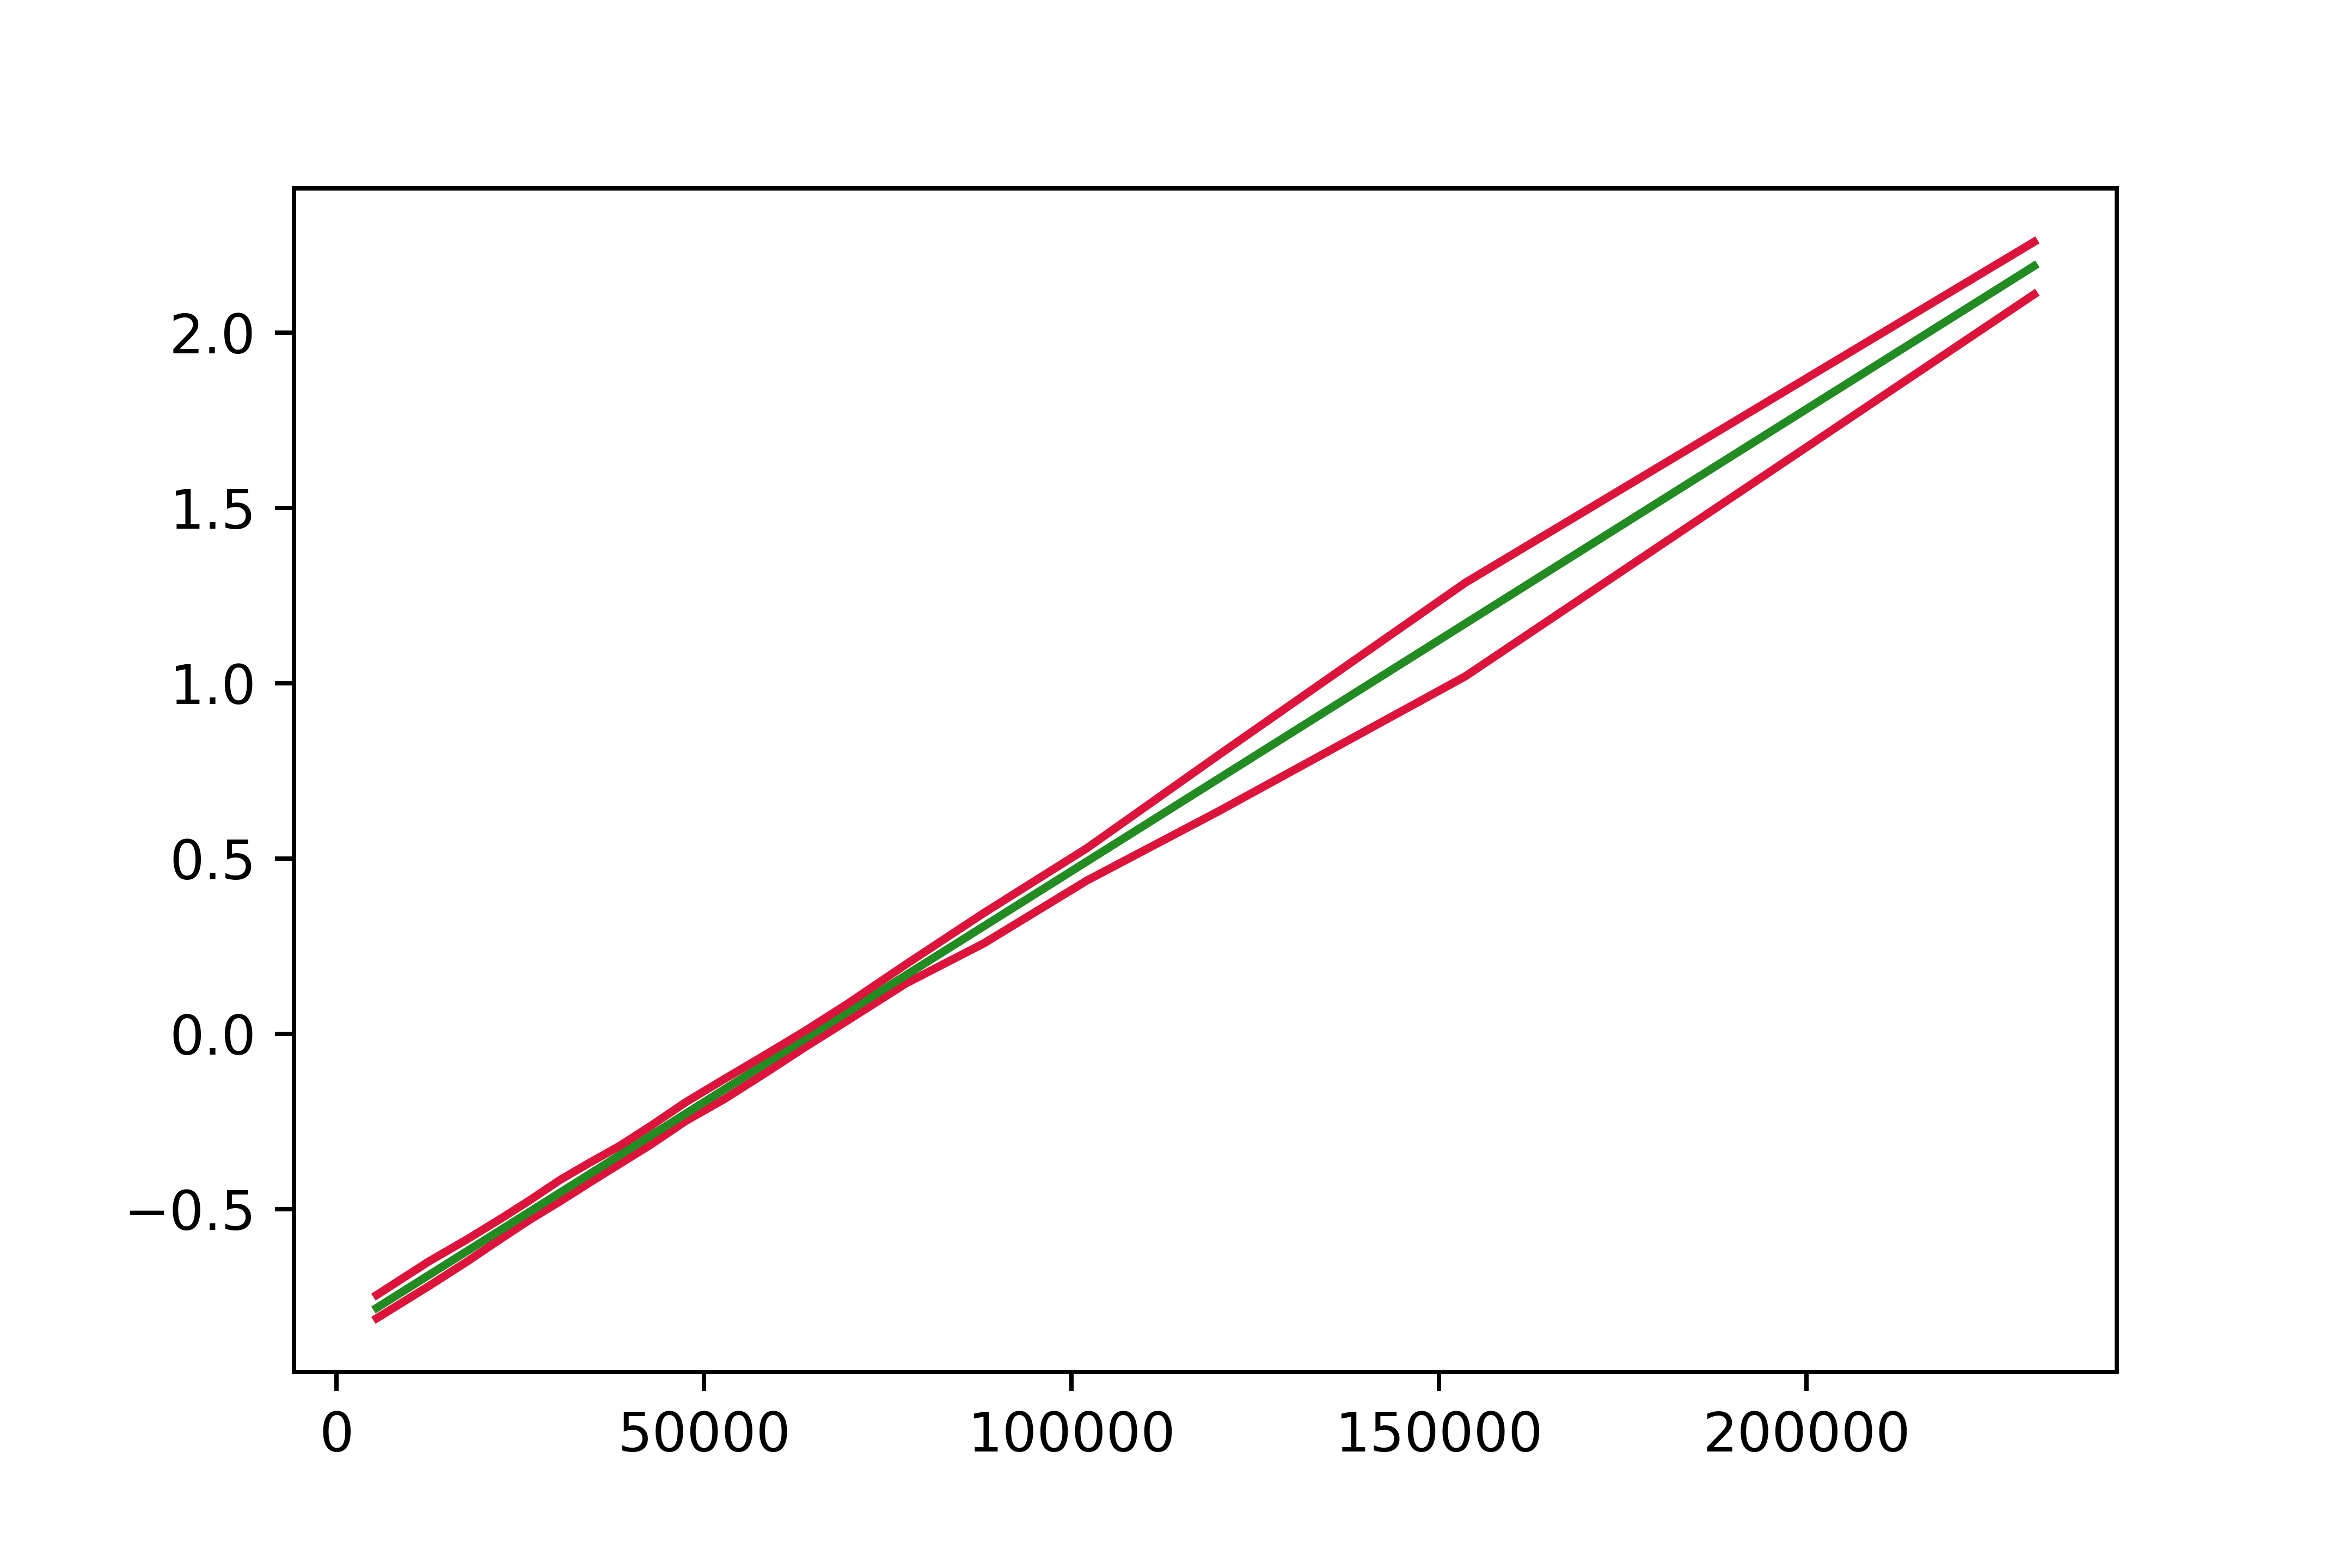
\includegraphics[width=\linewidth]{figures/ALE/chTOTexp/spec3_linear_FINCBTXM.png}
        \caption{Income - linear}
    \end{subfigure}%
    \begin{subfigure}{0.5\linewidth}
        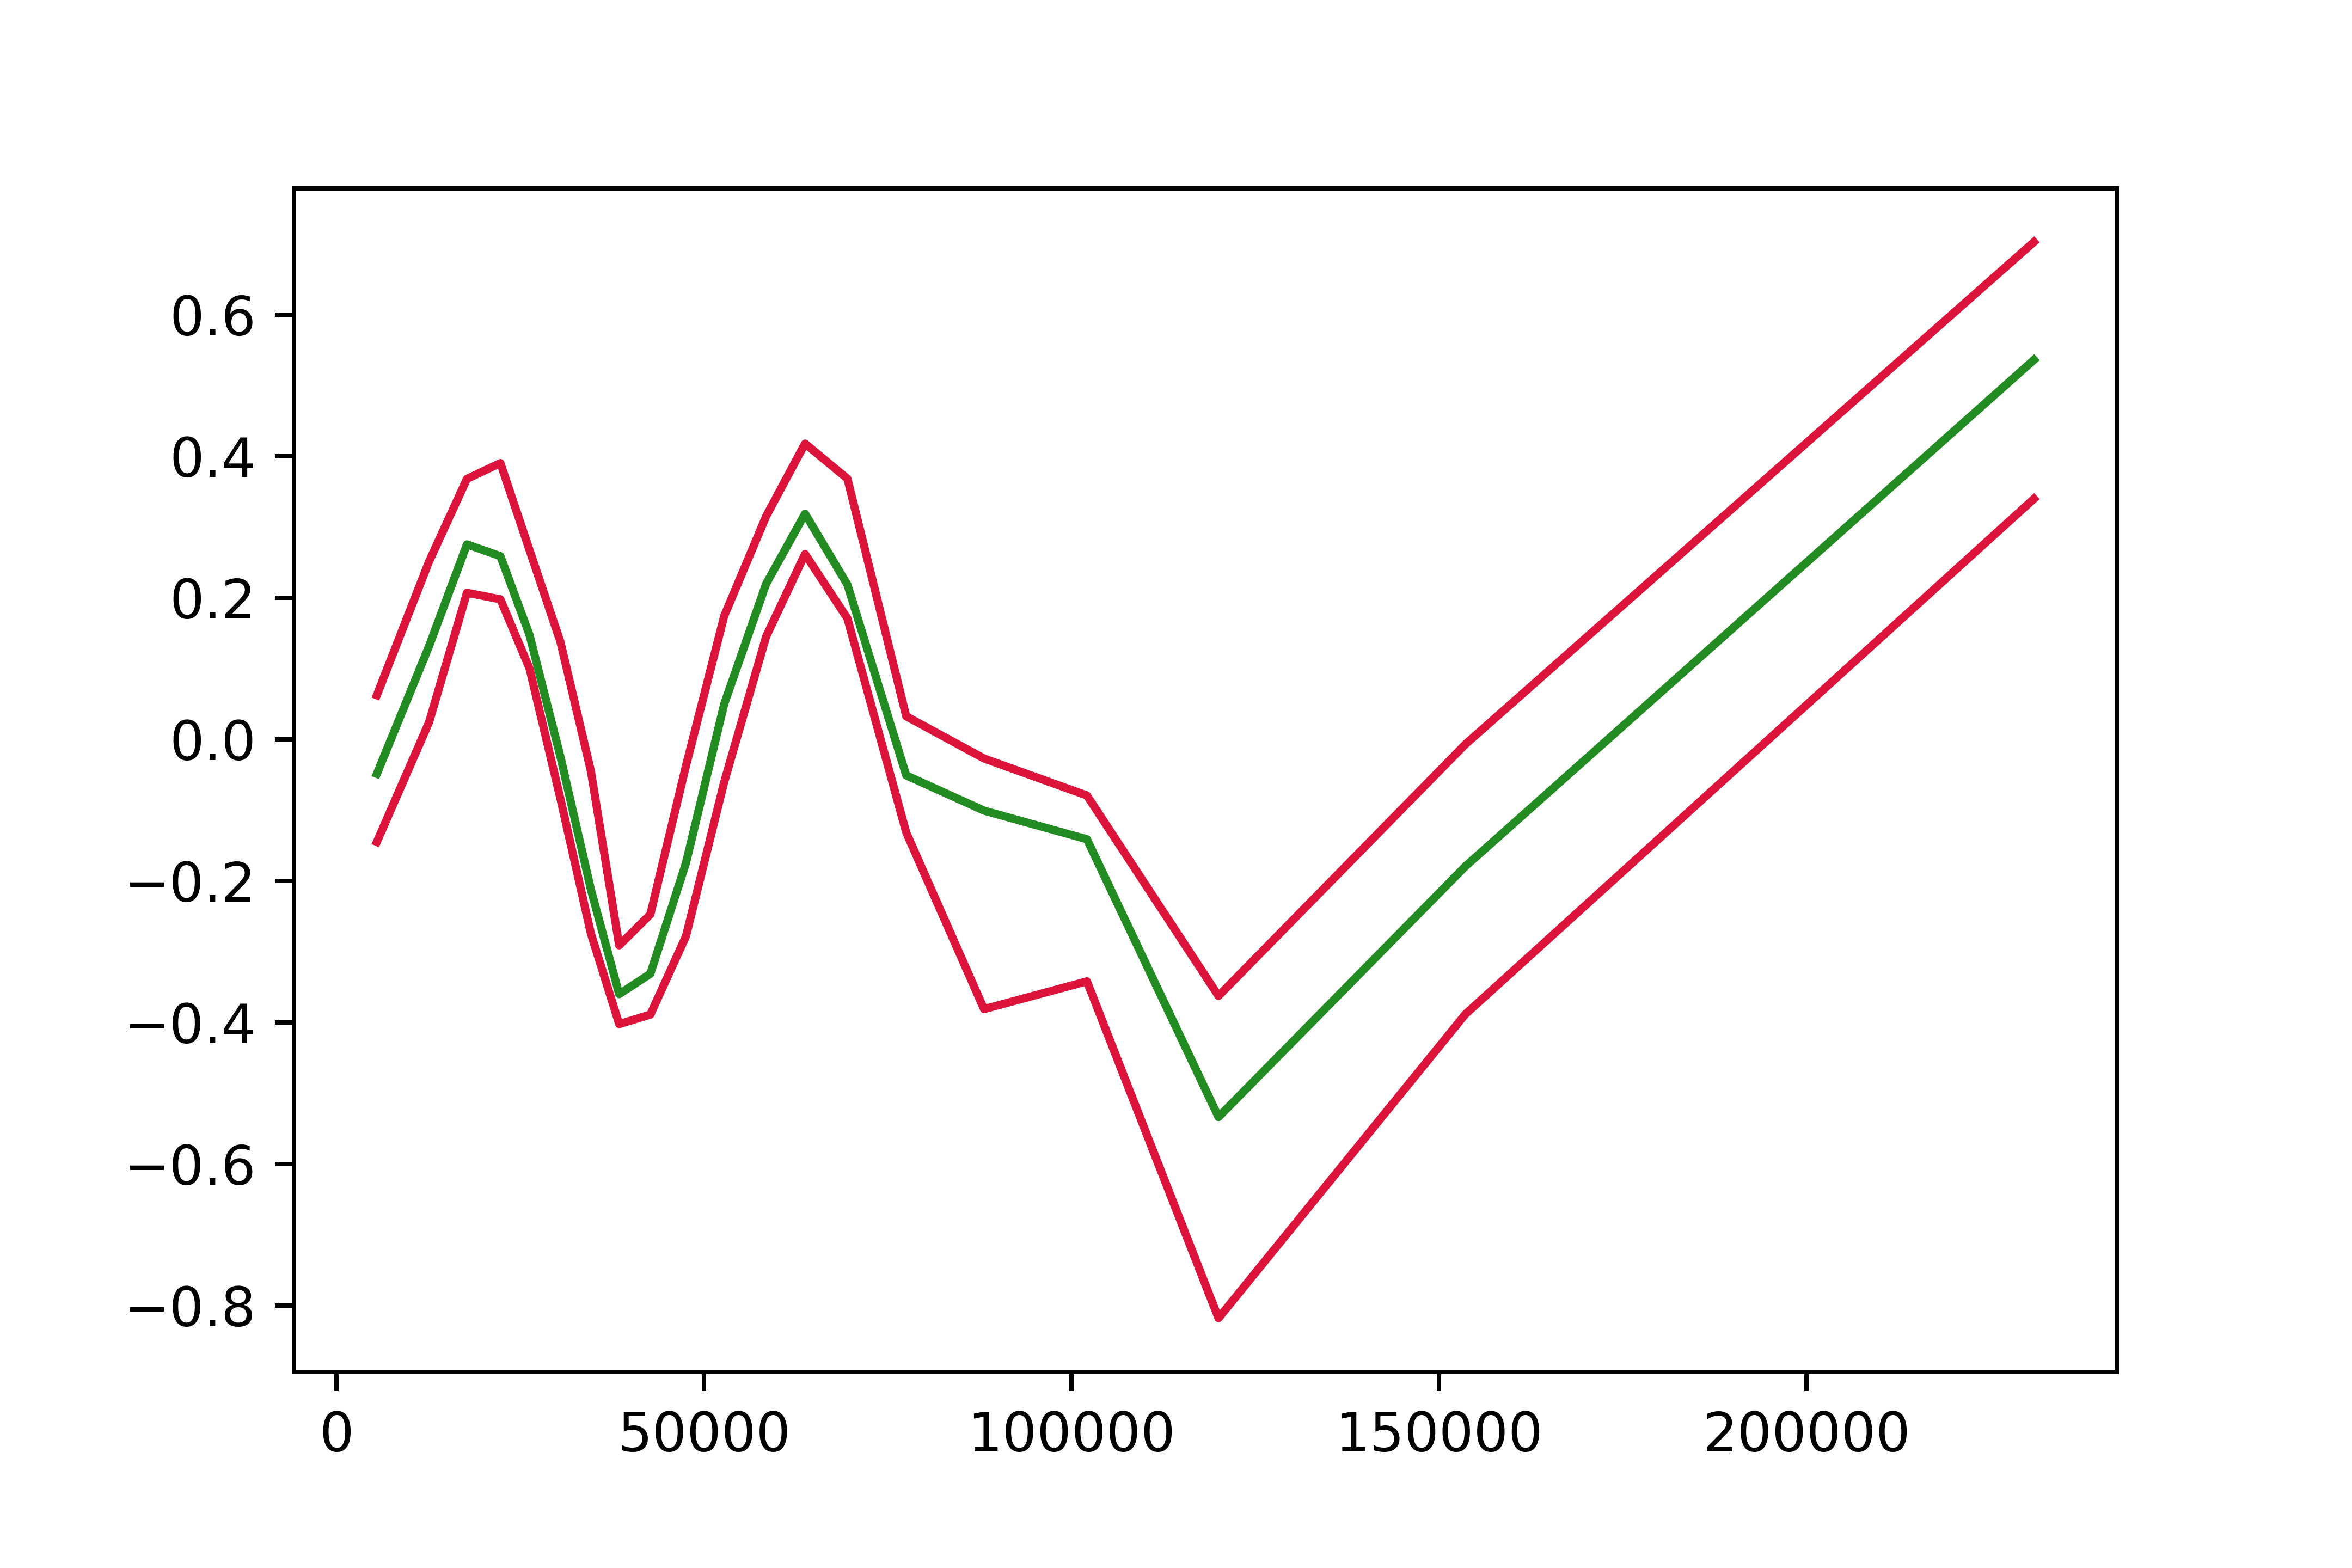
\includegraphics[width=\linewidth]{figures/ALE/chTOTexp/spec3_cf_FINCBTXM.png}
        \caption{Income - causal forest}
    \end{subfigure}
    \caption{ALE of \textit{financial status} variables - total expenditures}
    \label{app:ale_finstat_tot}
\end{figure}

%! SND - Age
\begin{figure}[h]
    \centering
    \begin{subfigure}{0.5\linewidth}
        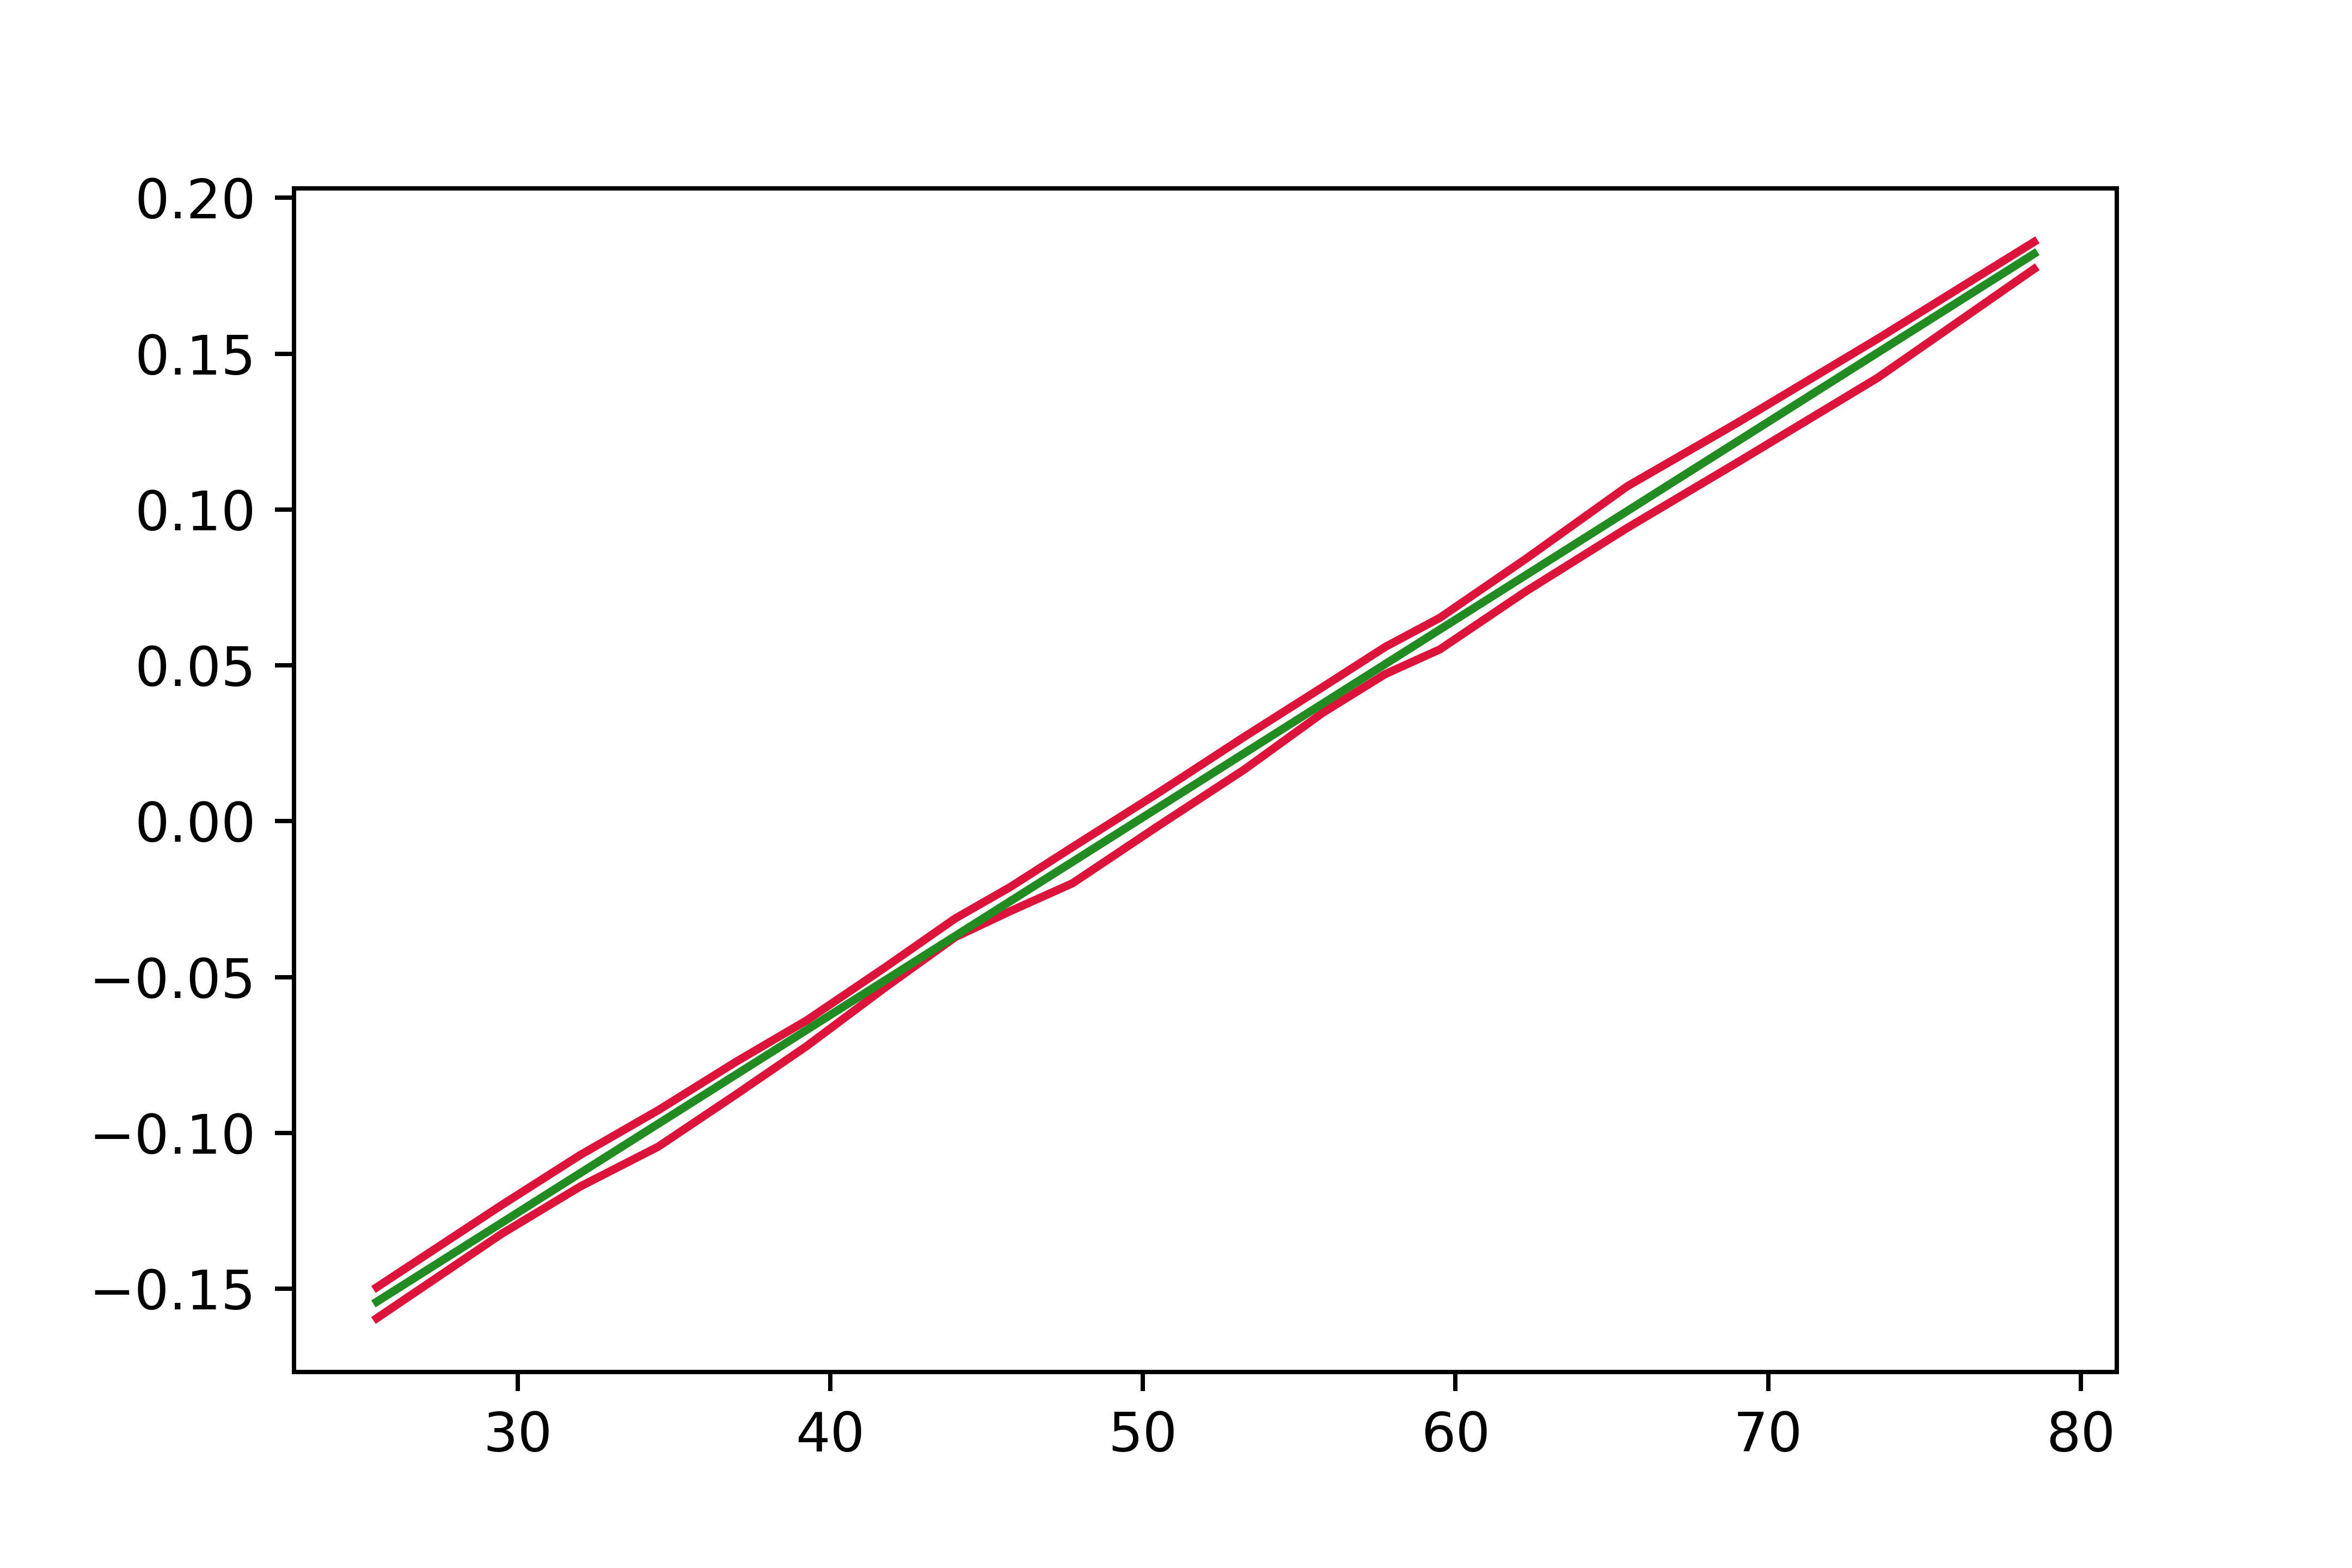
\includegraphics[width=\linewidth]{figures/ALE/chSNDexp/spec1_linear_AGE.png}
        \caption{Spec 1 - linear}
    \end{subfigure}%
    \begin{subfigure}{0.5\linewidth}
        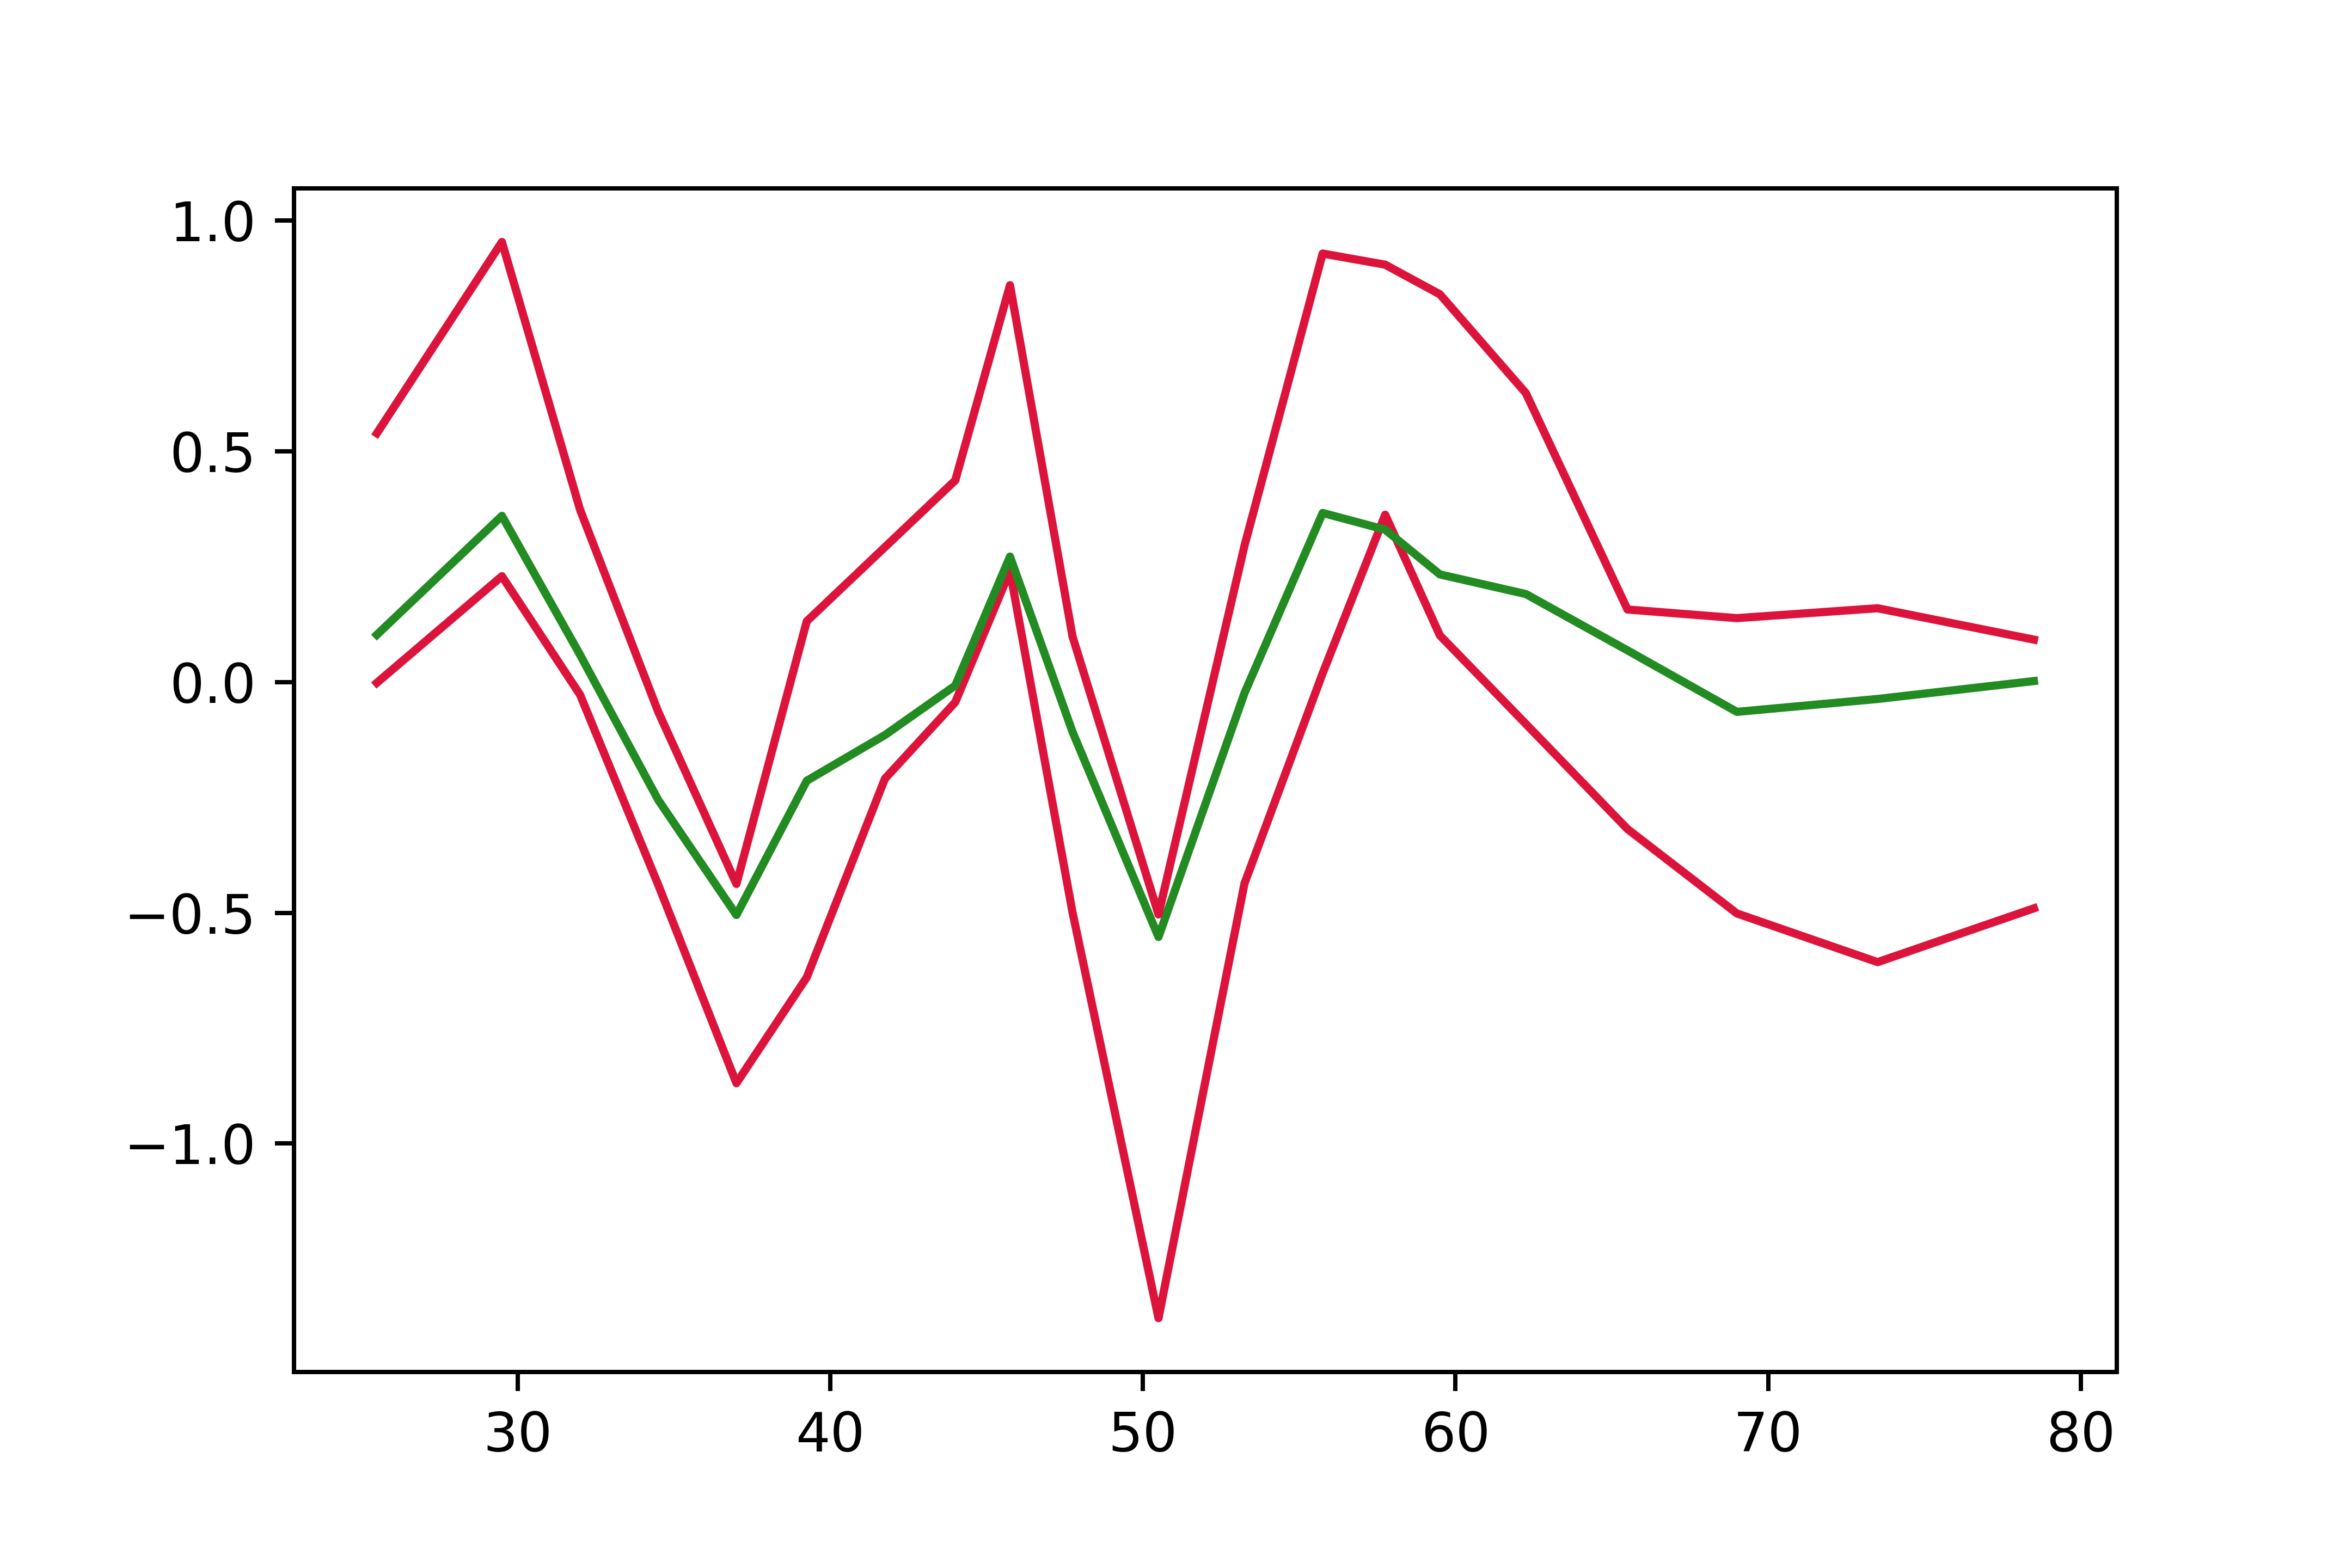
\includegraphics[width=\linewidth]{figures/ALE/chSNDexp/spec1_cf_AGE.png}
        \caption{Spec 1 - causal forest}
    \end{subfigure}

    \begin{subfigure}{0.5\linewidth}
        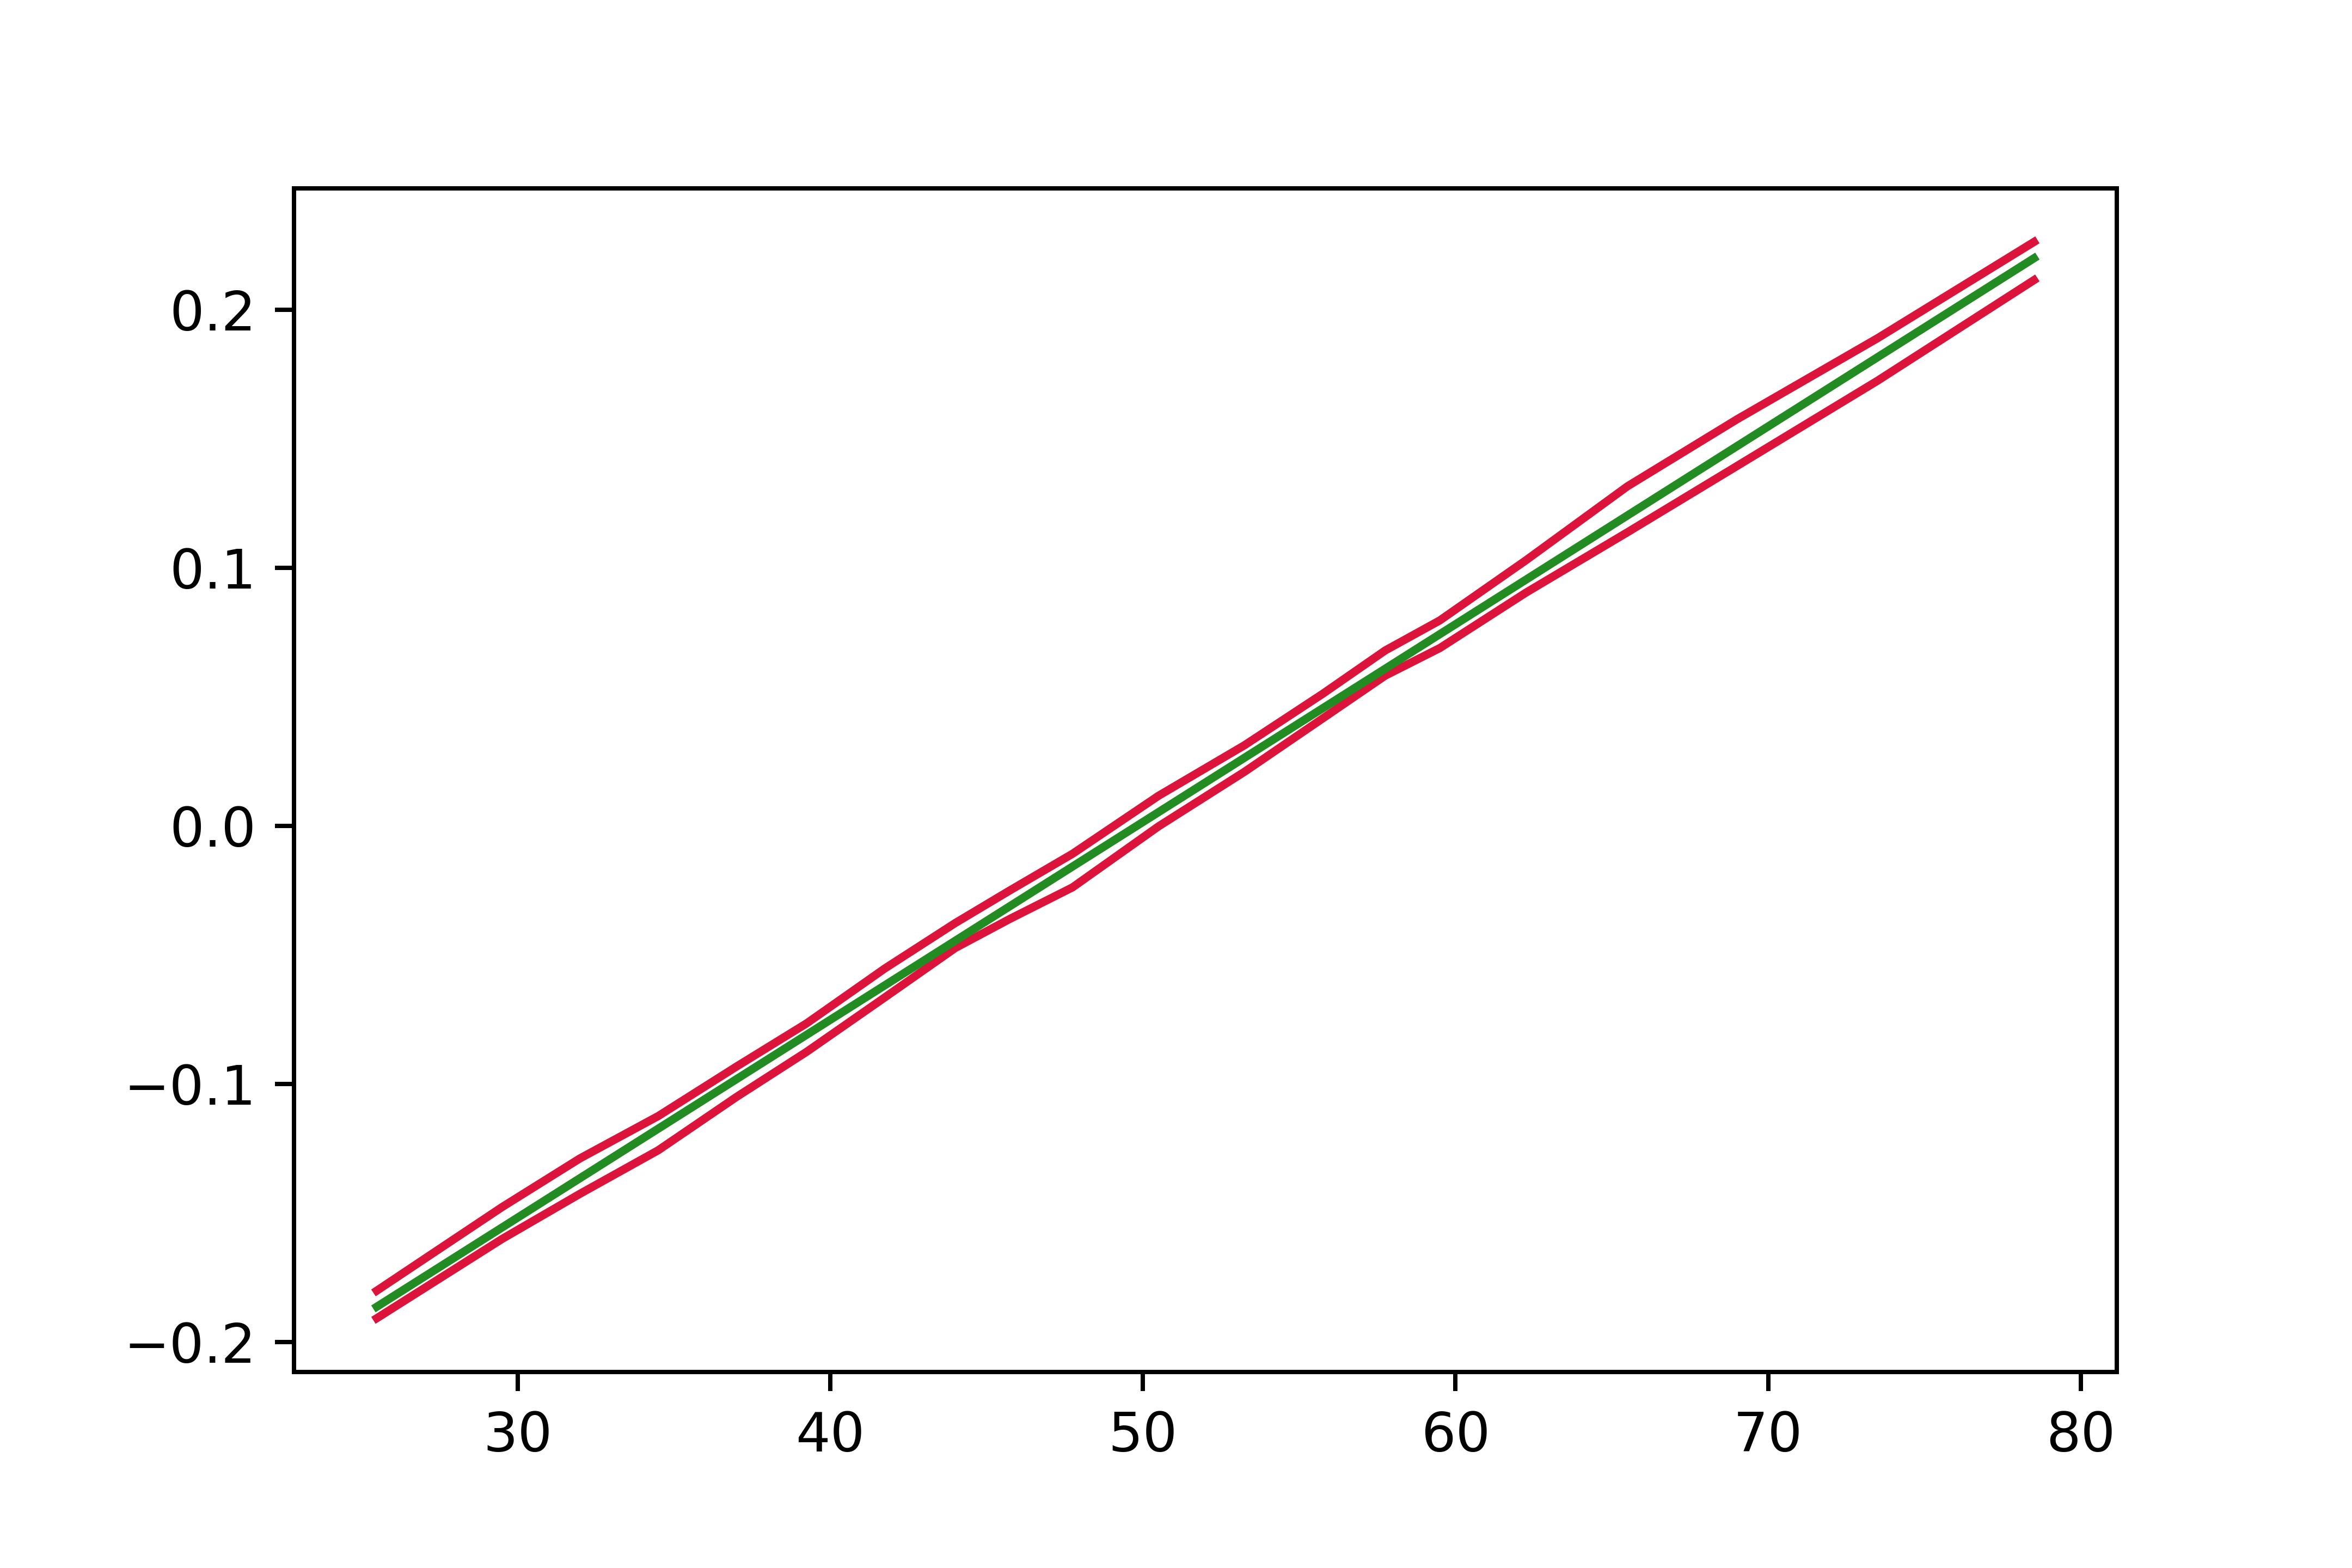
\includegraphics[width=\linewidth]{figures/ALE/chSNDexp/spec2_linear_AGE.png}
        \caption{Spec 2 - linear}
    \end{subfigure}%
    \begin{subfigure}{0.5\linewidth}
        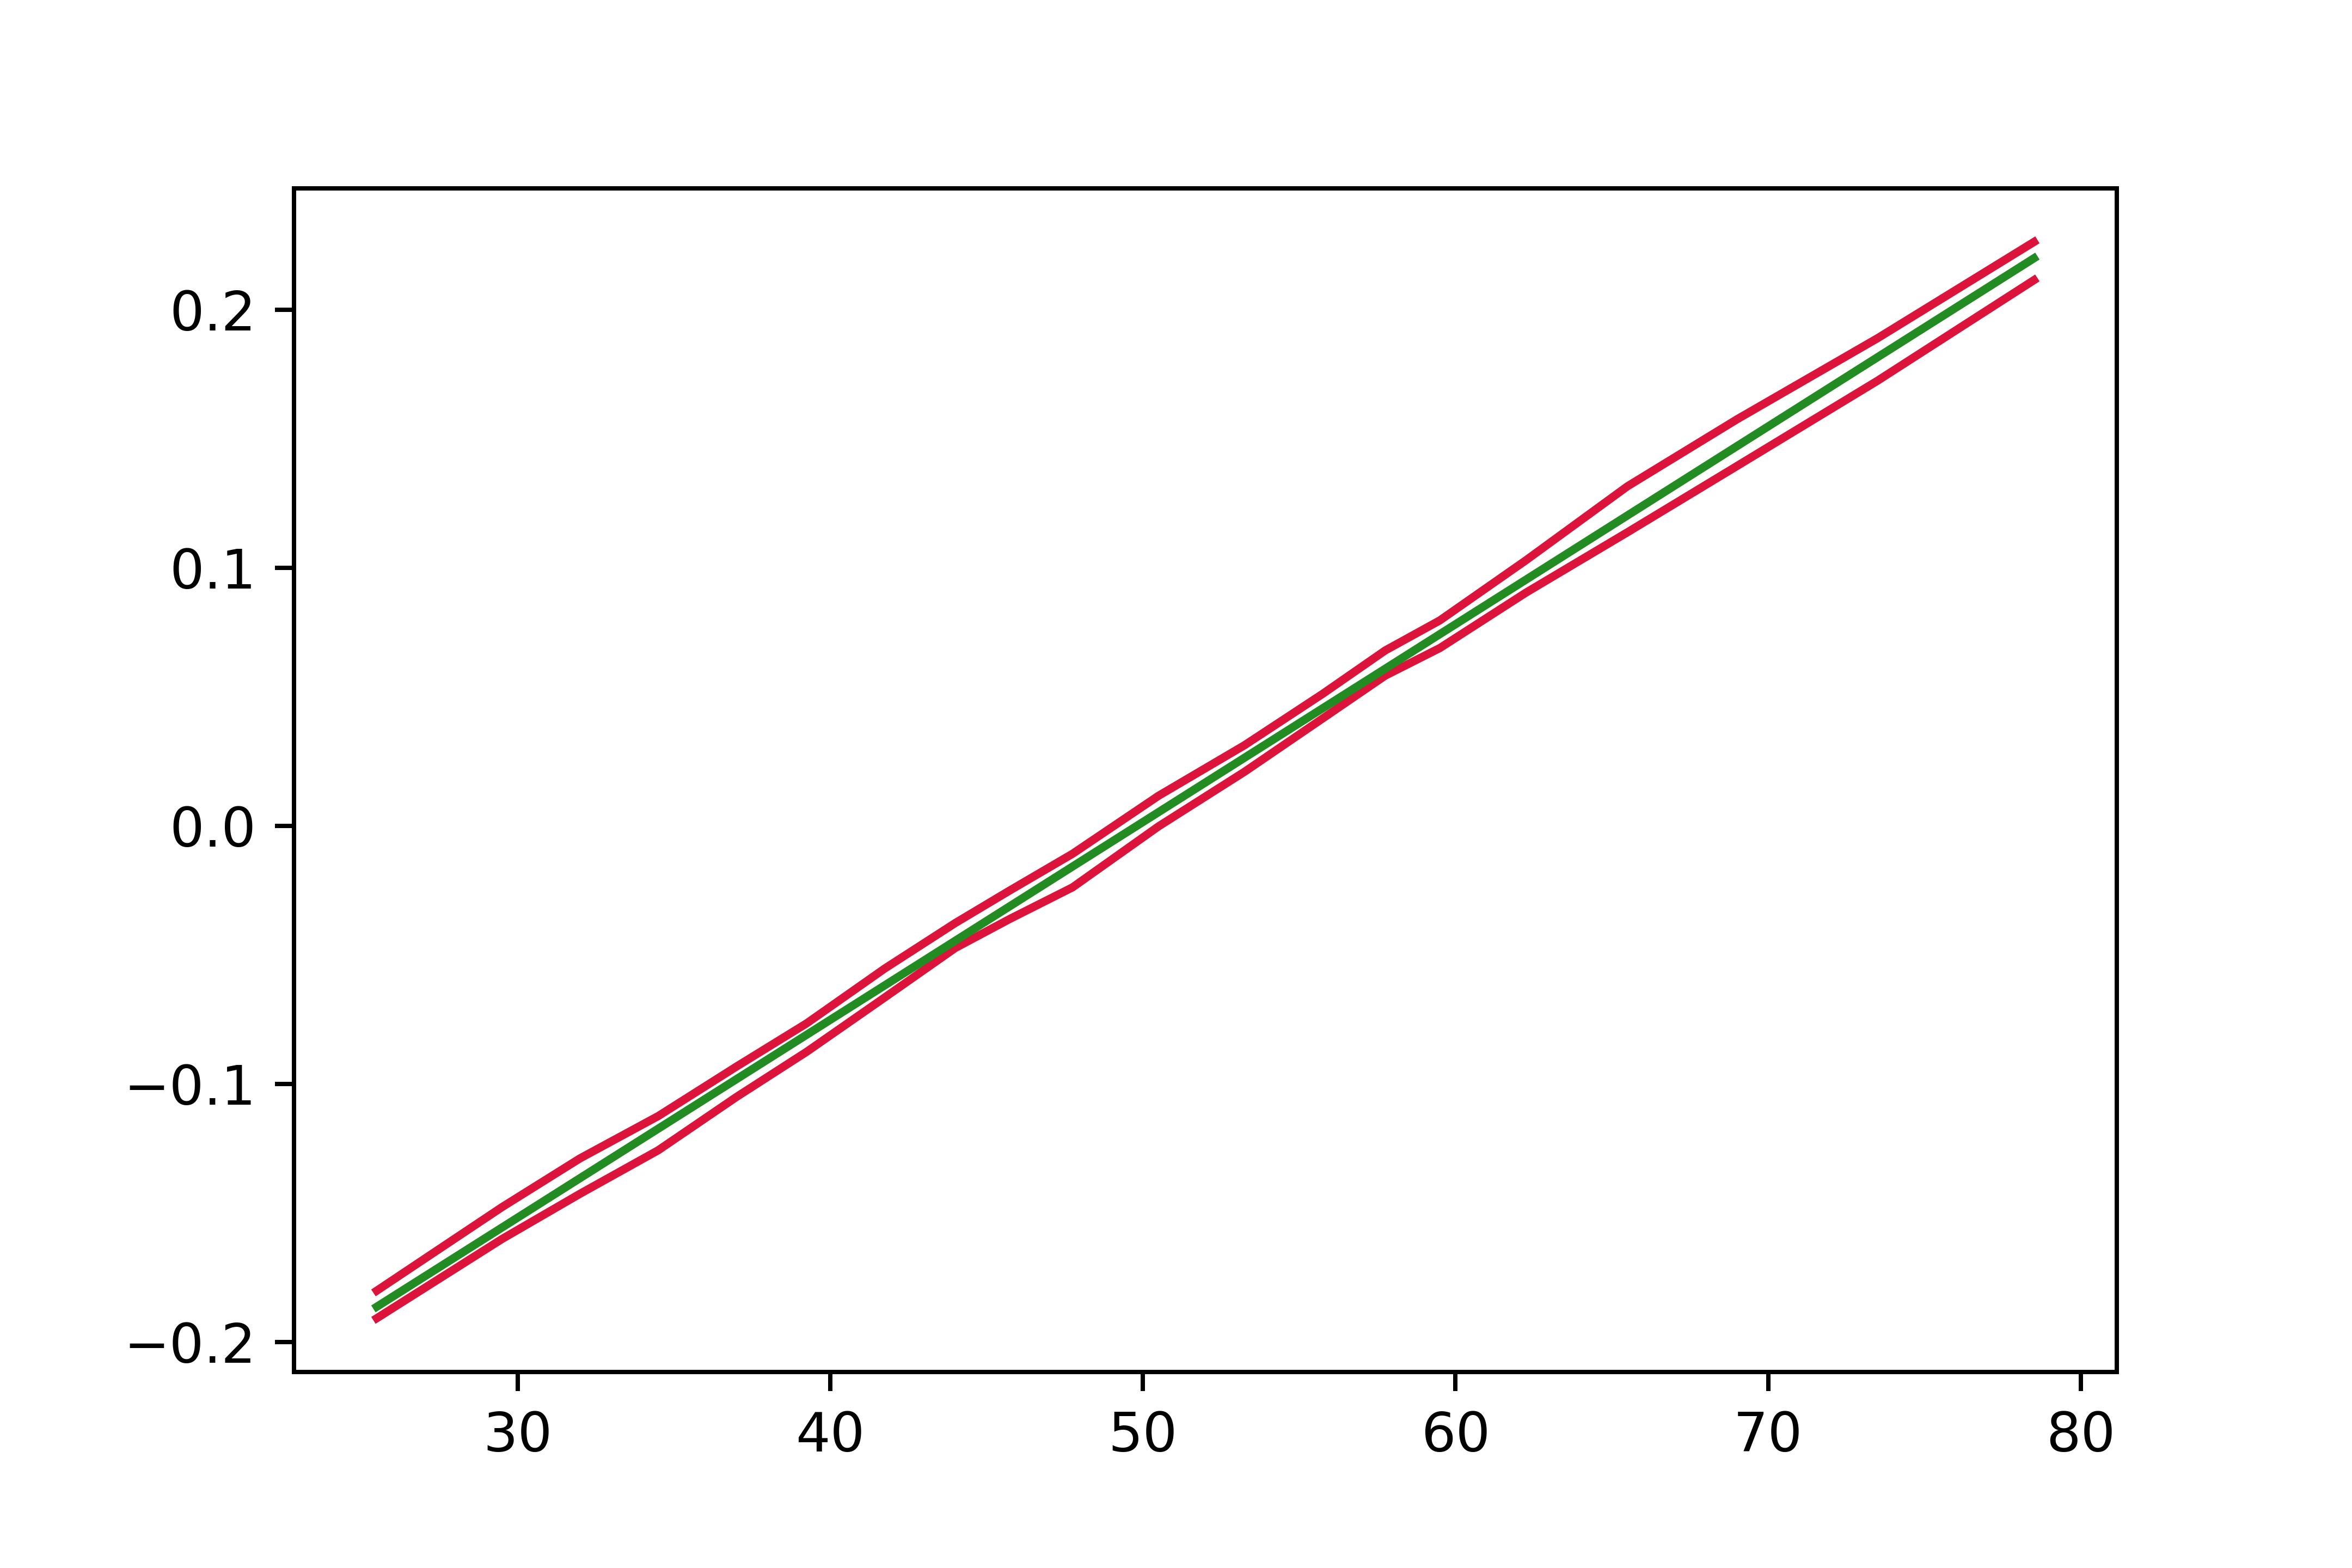
\includegraphics[width=\linewidth]{figures/ALE/chSNDexp/spec2_linear_AGE.png}
        \caption{Spec 2 - causal forest}
    \end{subfigure}

    \begin{subfigure}{0.5\linewidth}
        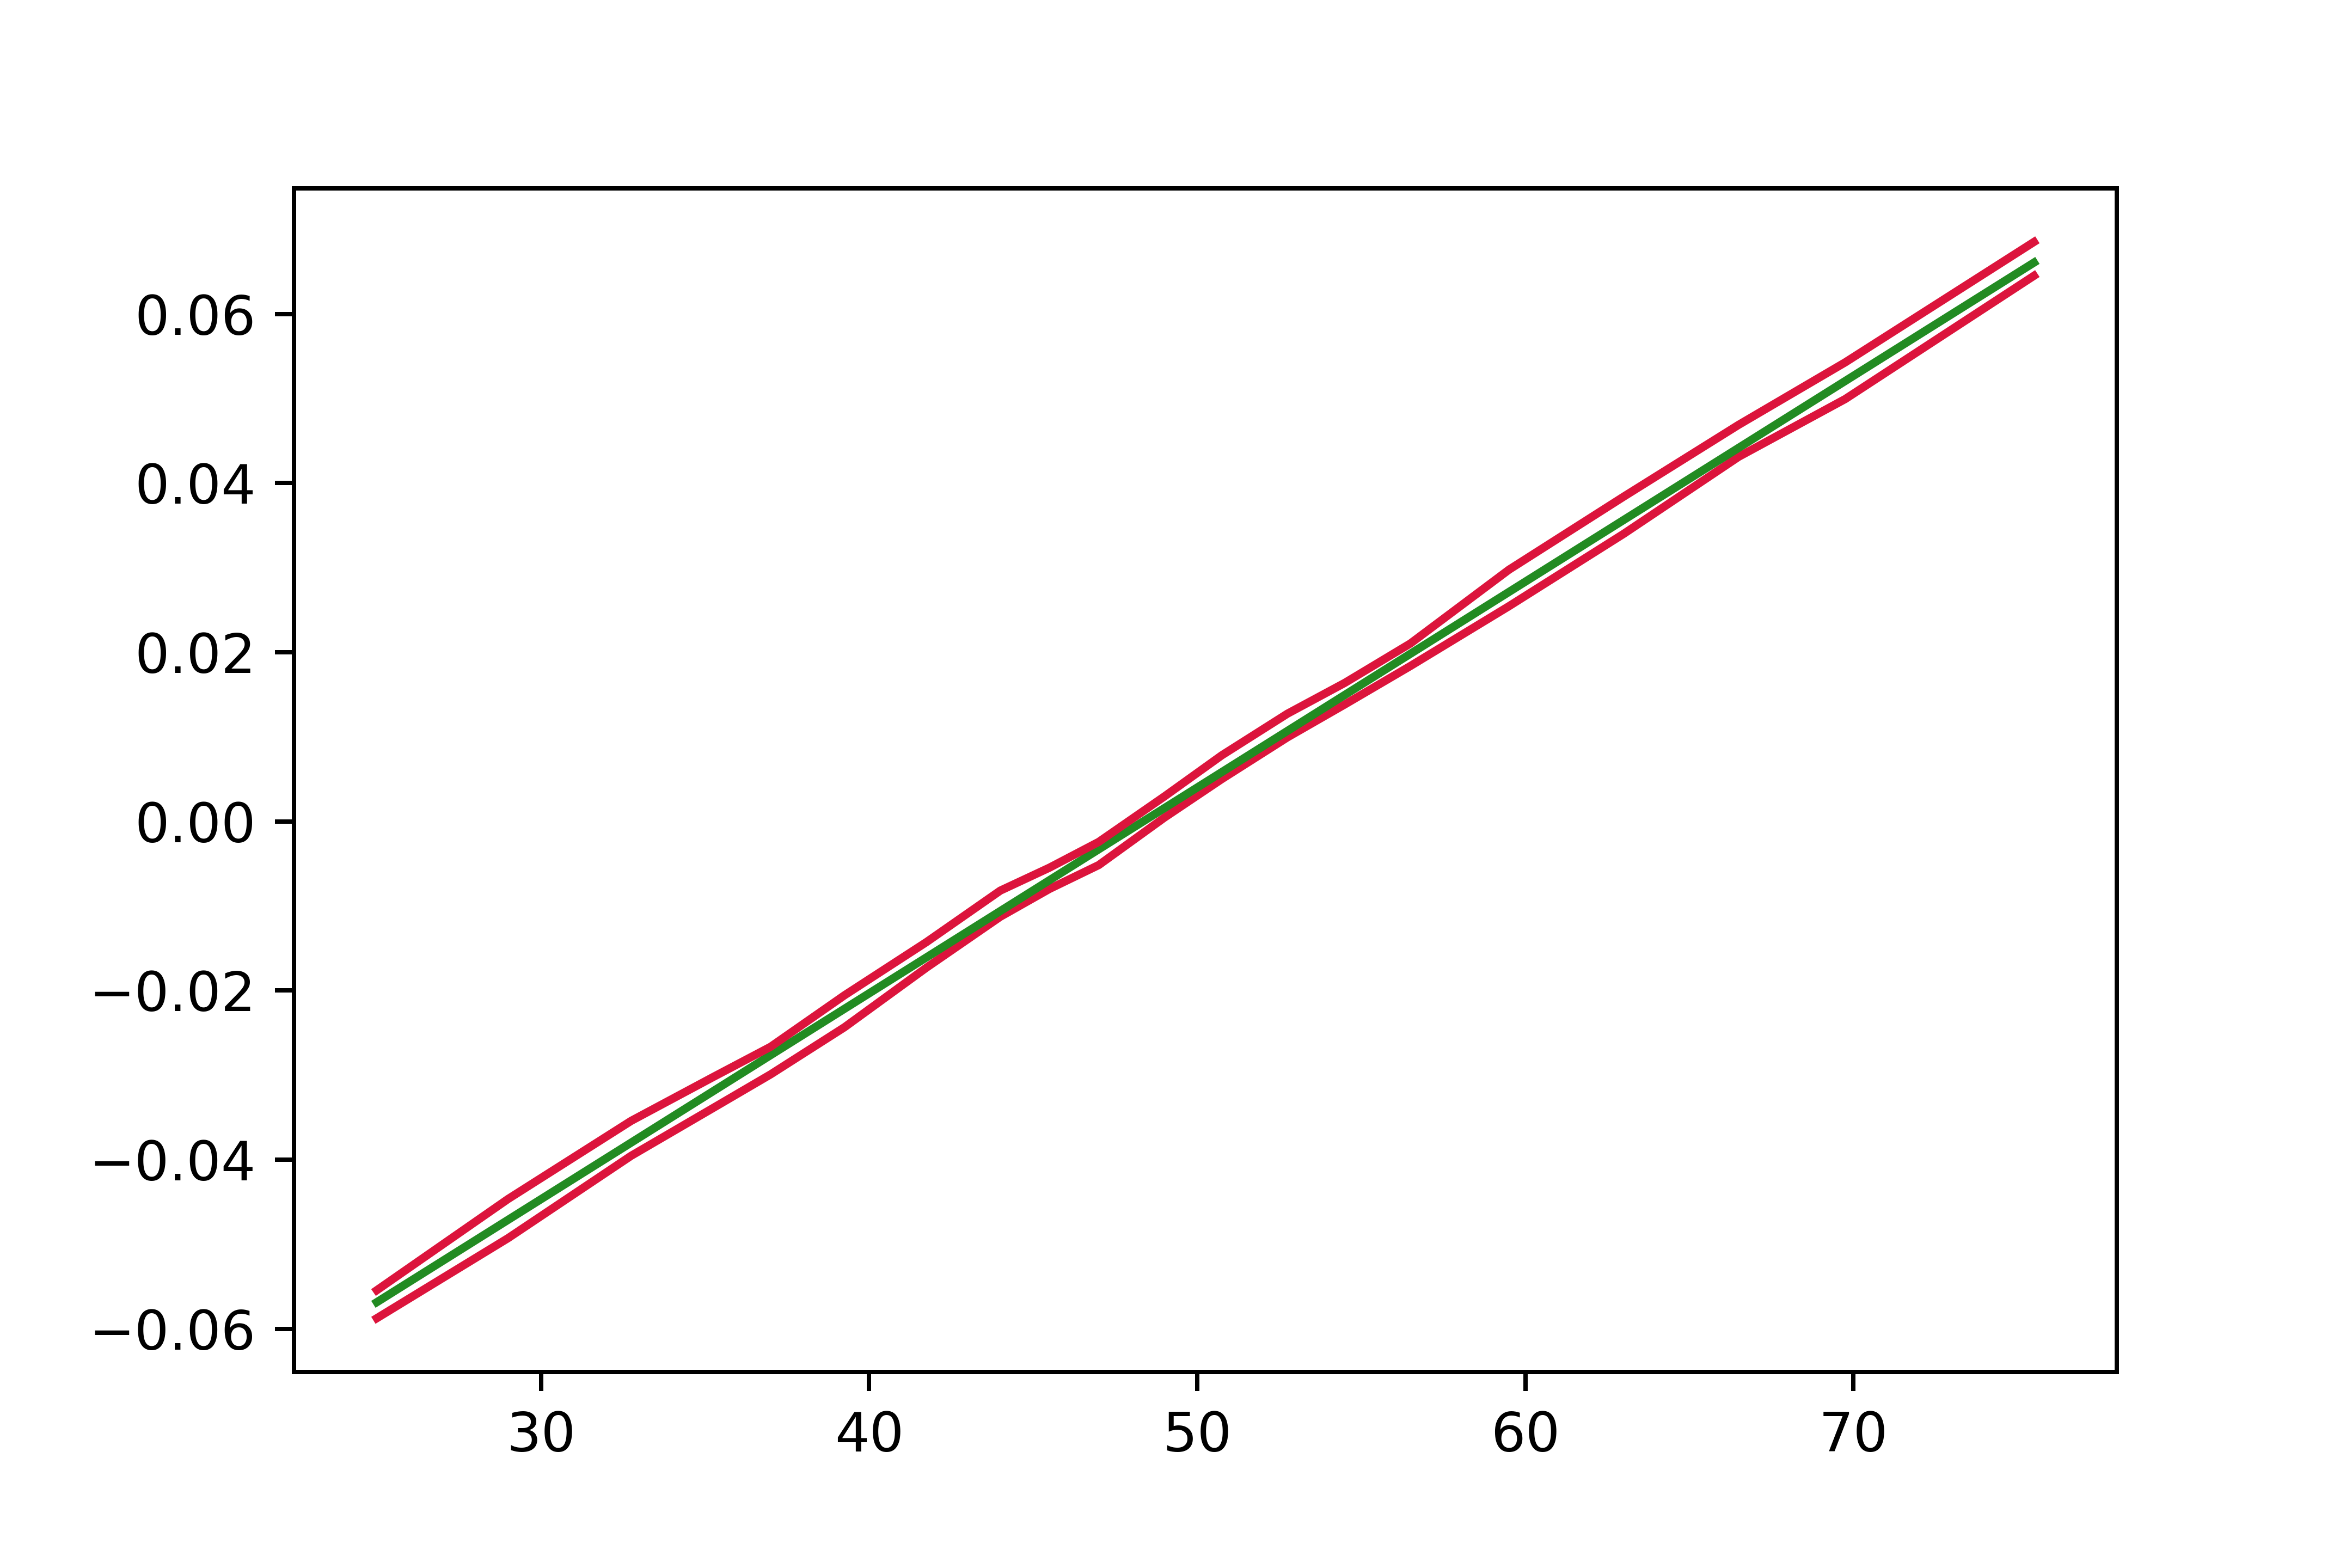
\includegraphics[width=\linewidth]{figures/ALE/chSNDexp/spec3_linear_AGE.png}
        \caption{Spec 3 - linear}
    \end{subfigure}%
    \begin{subfigure}{0.5\linewidth}
        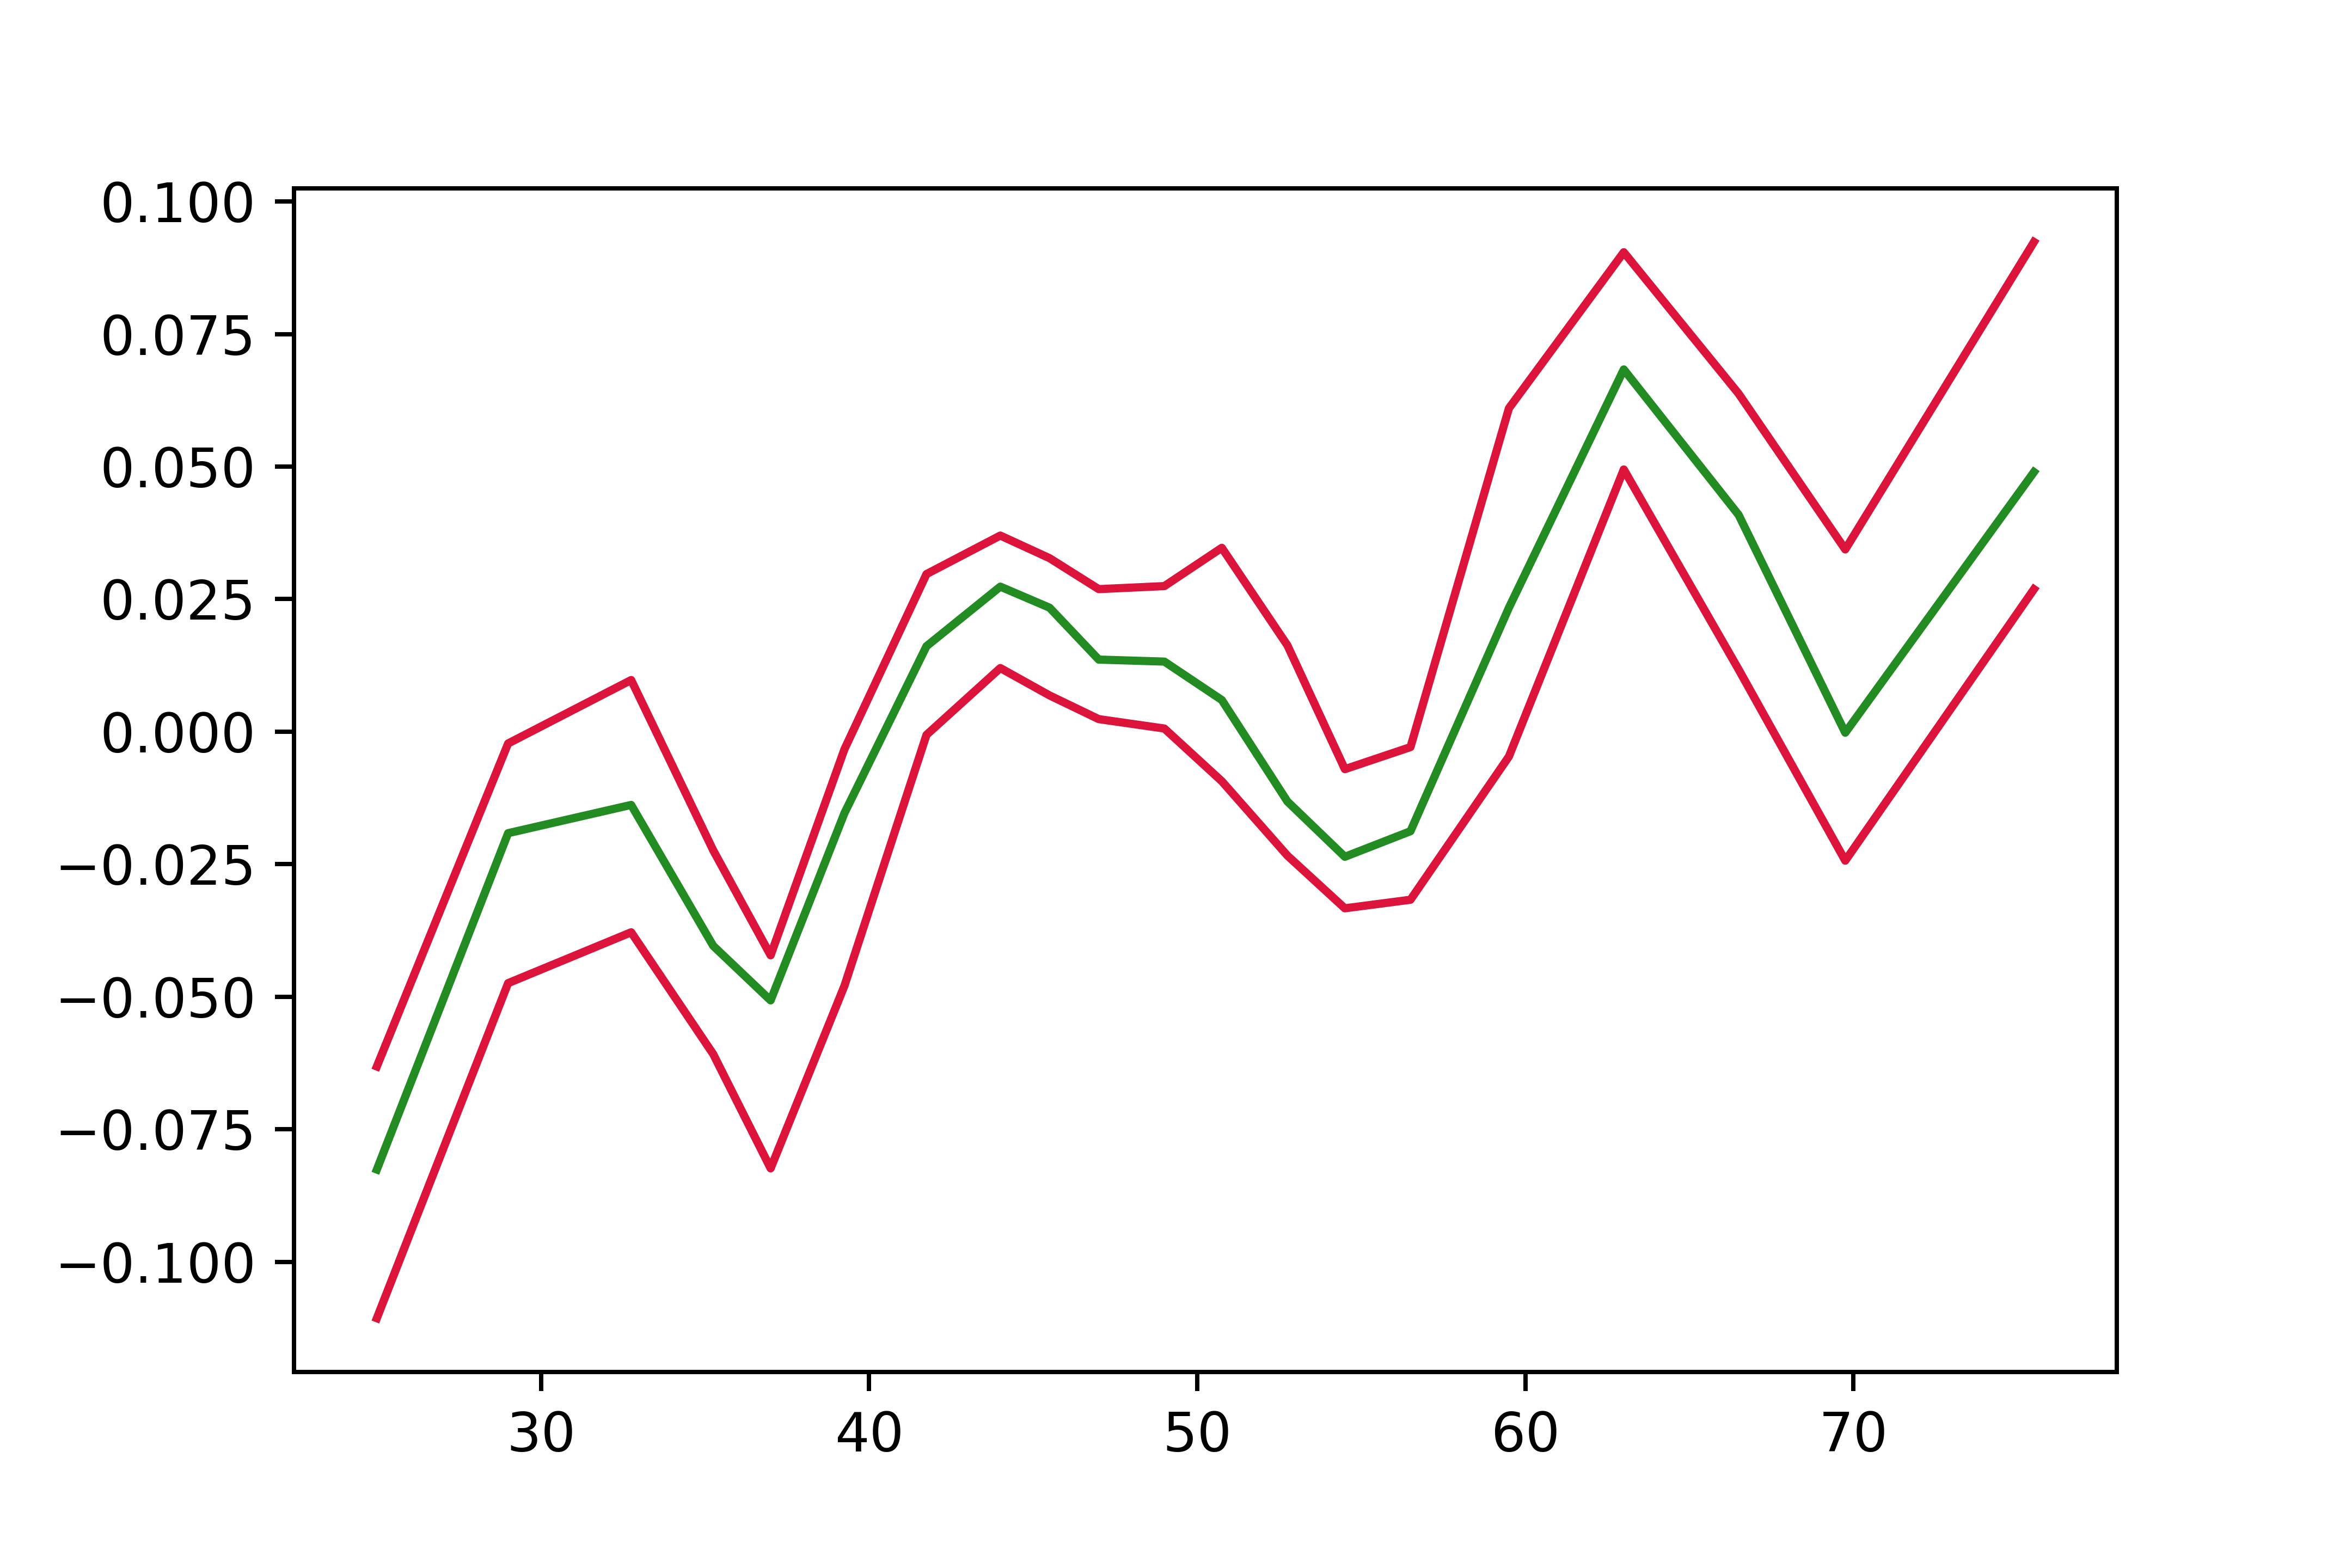
\includegraphics[width=\linewidth]{figures/ALE/chSNDexp/spec3_cf_AGE.png}
        \caption{Spec 3 - causal forest}
    \end{subfigure}
    \caption{ALE of AGE - strictly non-durables}
    \label{app:ale_age_snd}
\end{figure}

%! SND - Fin Stat
\begin{figure}[h]
    \centering
    \begin{subfigure}{0.5\linewidth}
        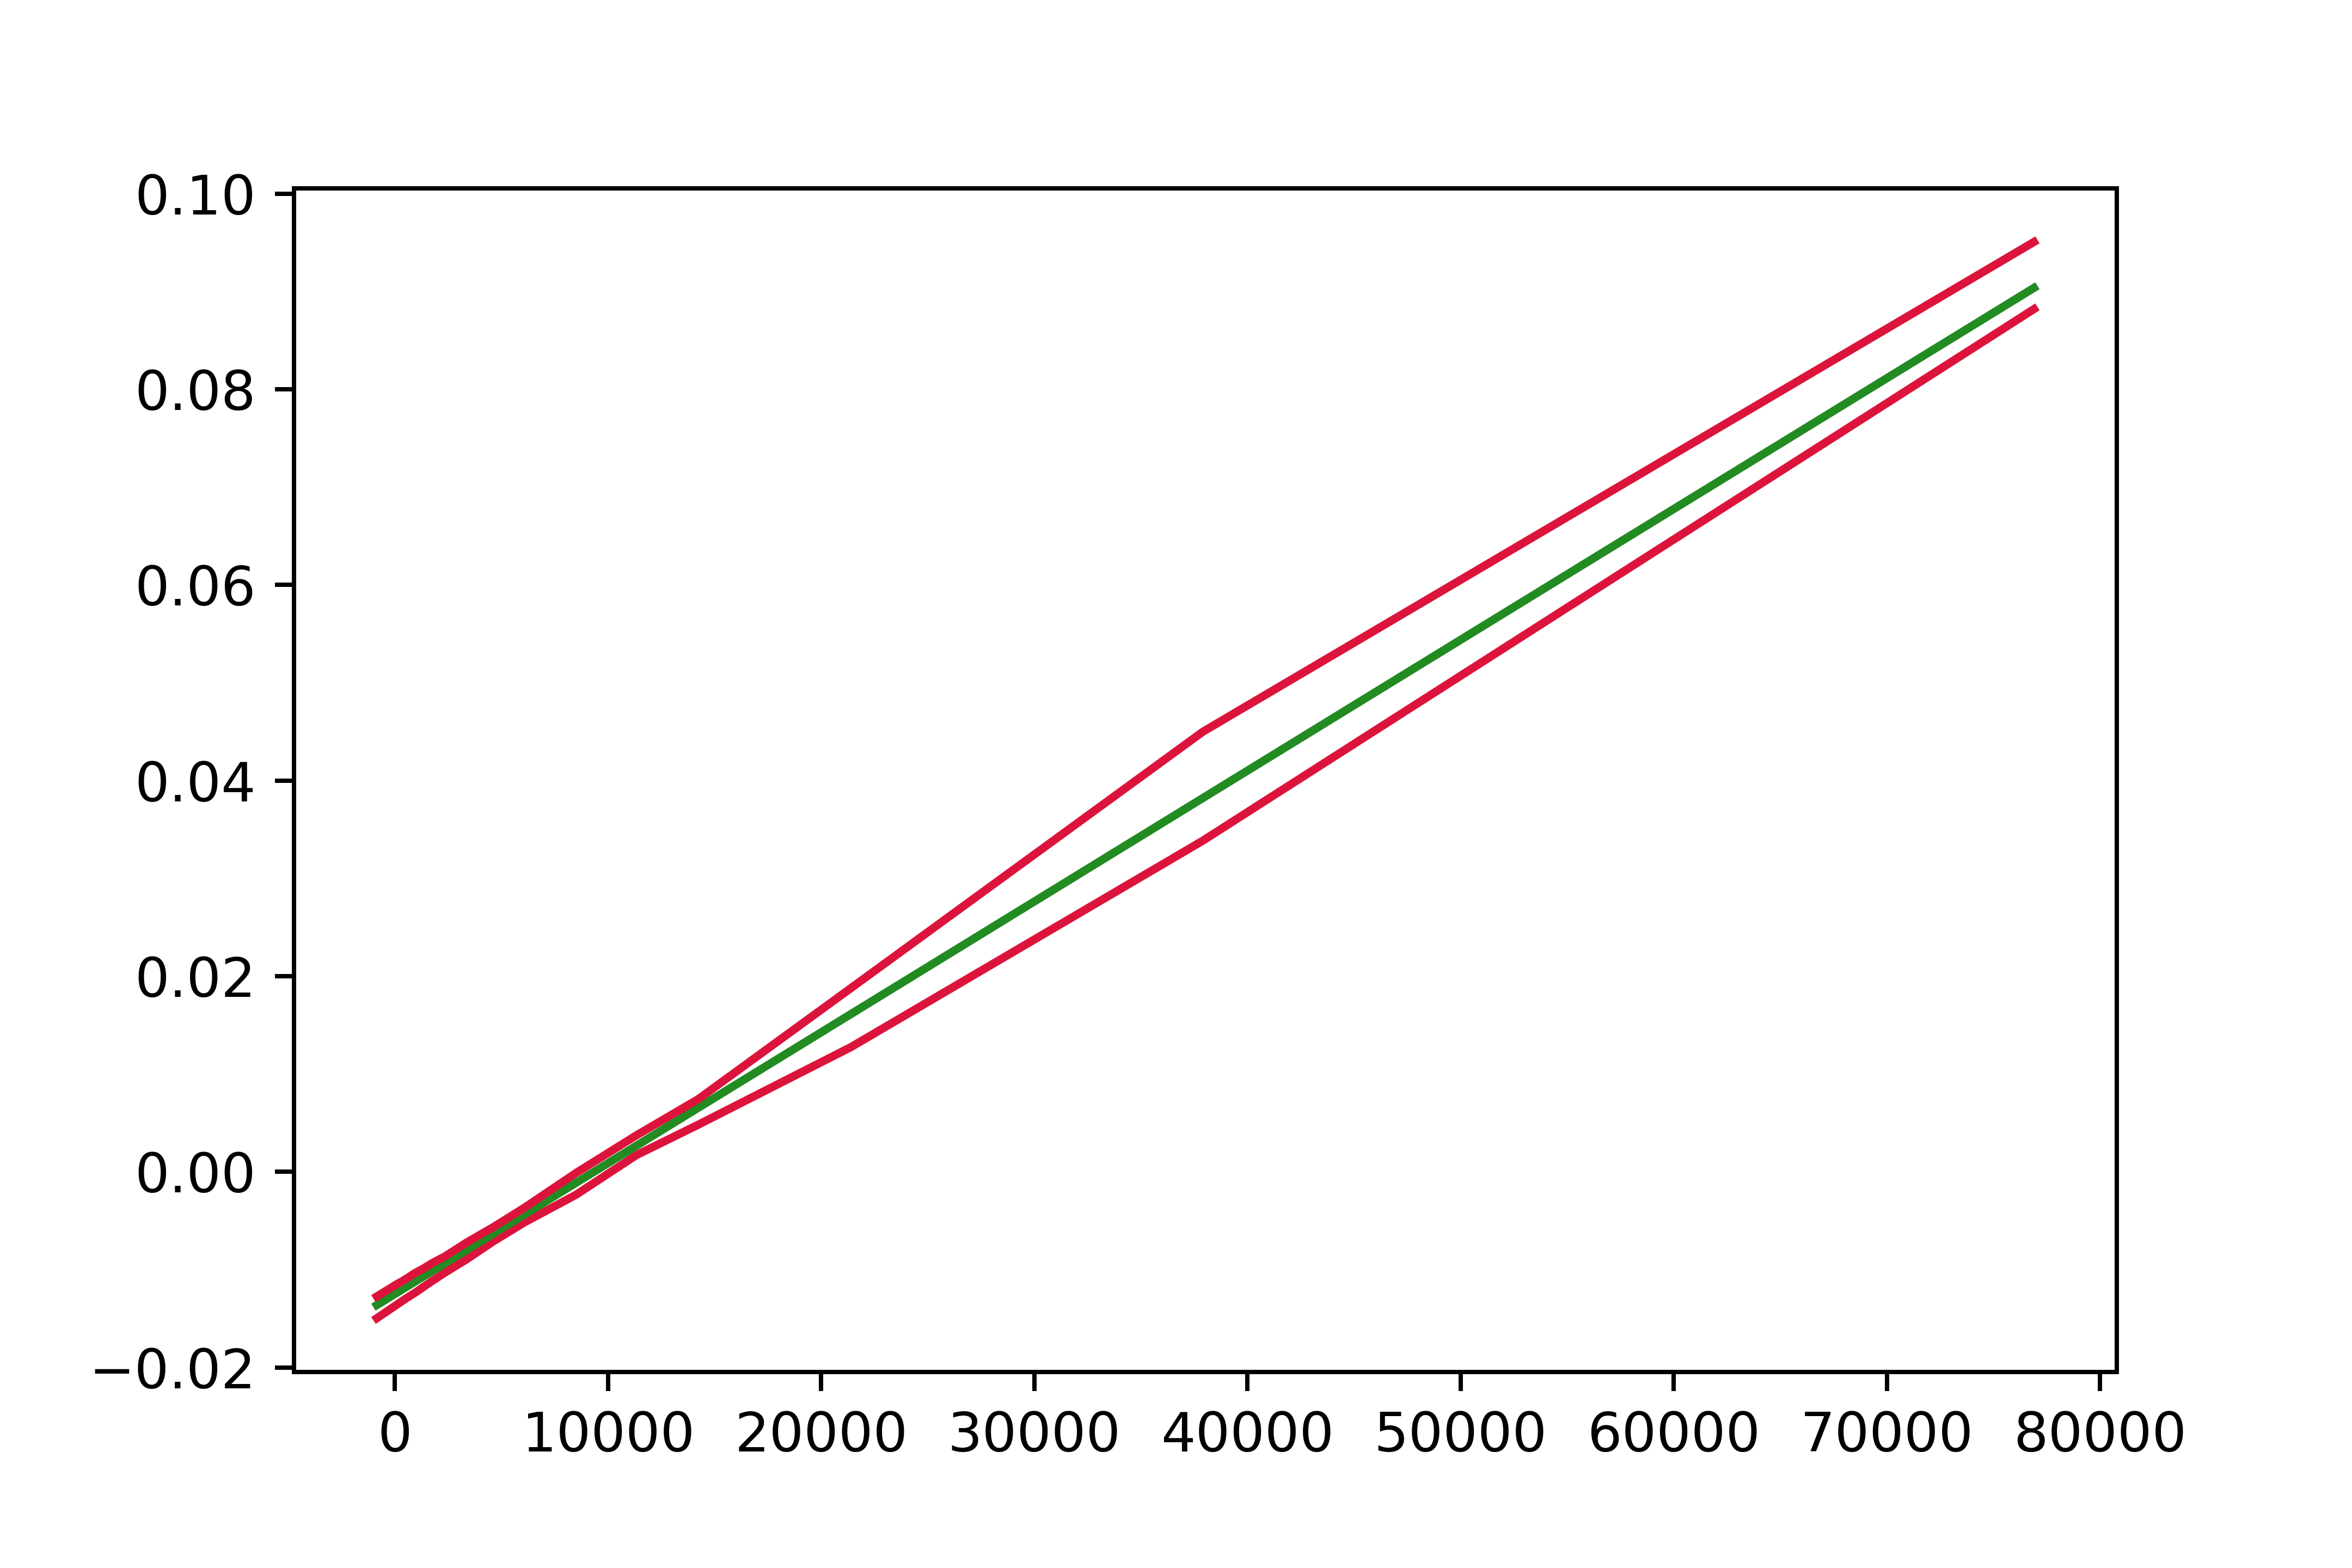
\includegraphics[width=\linewidth]{figures/ALE/chSNDexp/spec3_linear_liqassii.png}
        \caption{Liquid Assets - linear}
    \end{subfigure}%
    \begin{subfigure}{0.5\linewidth}
        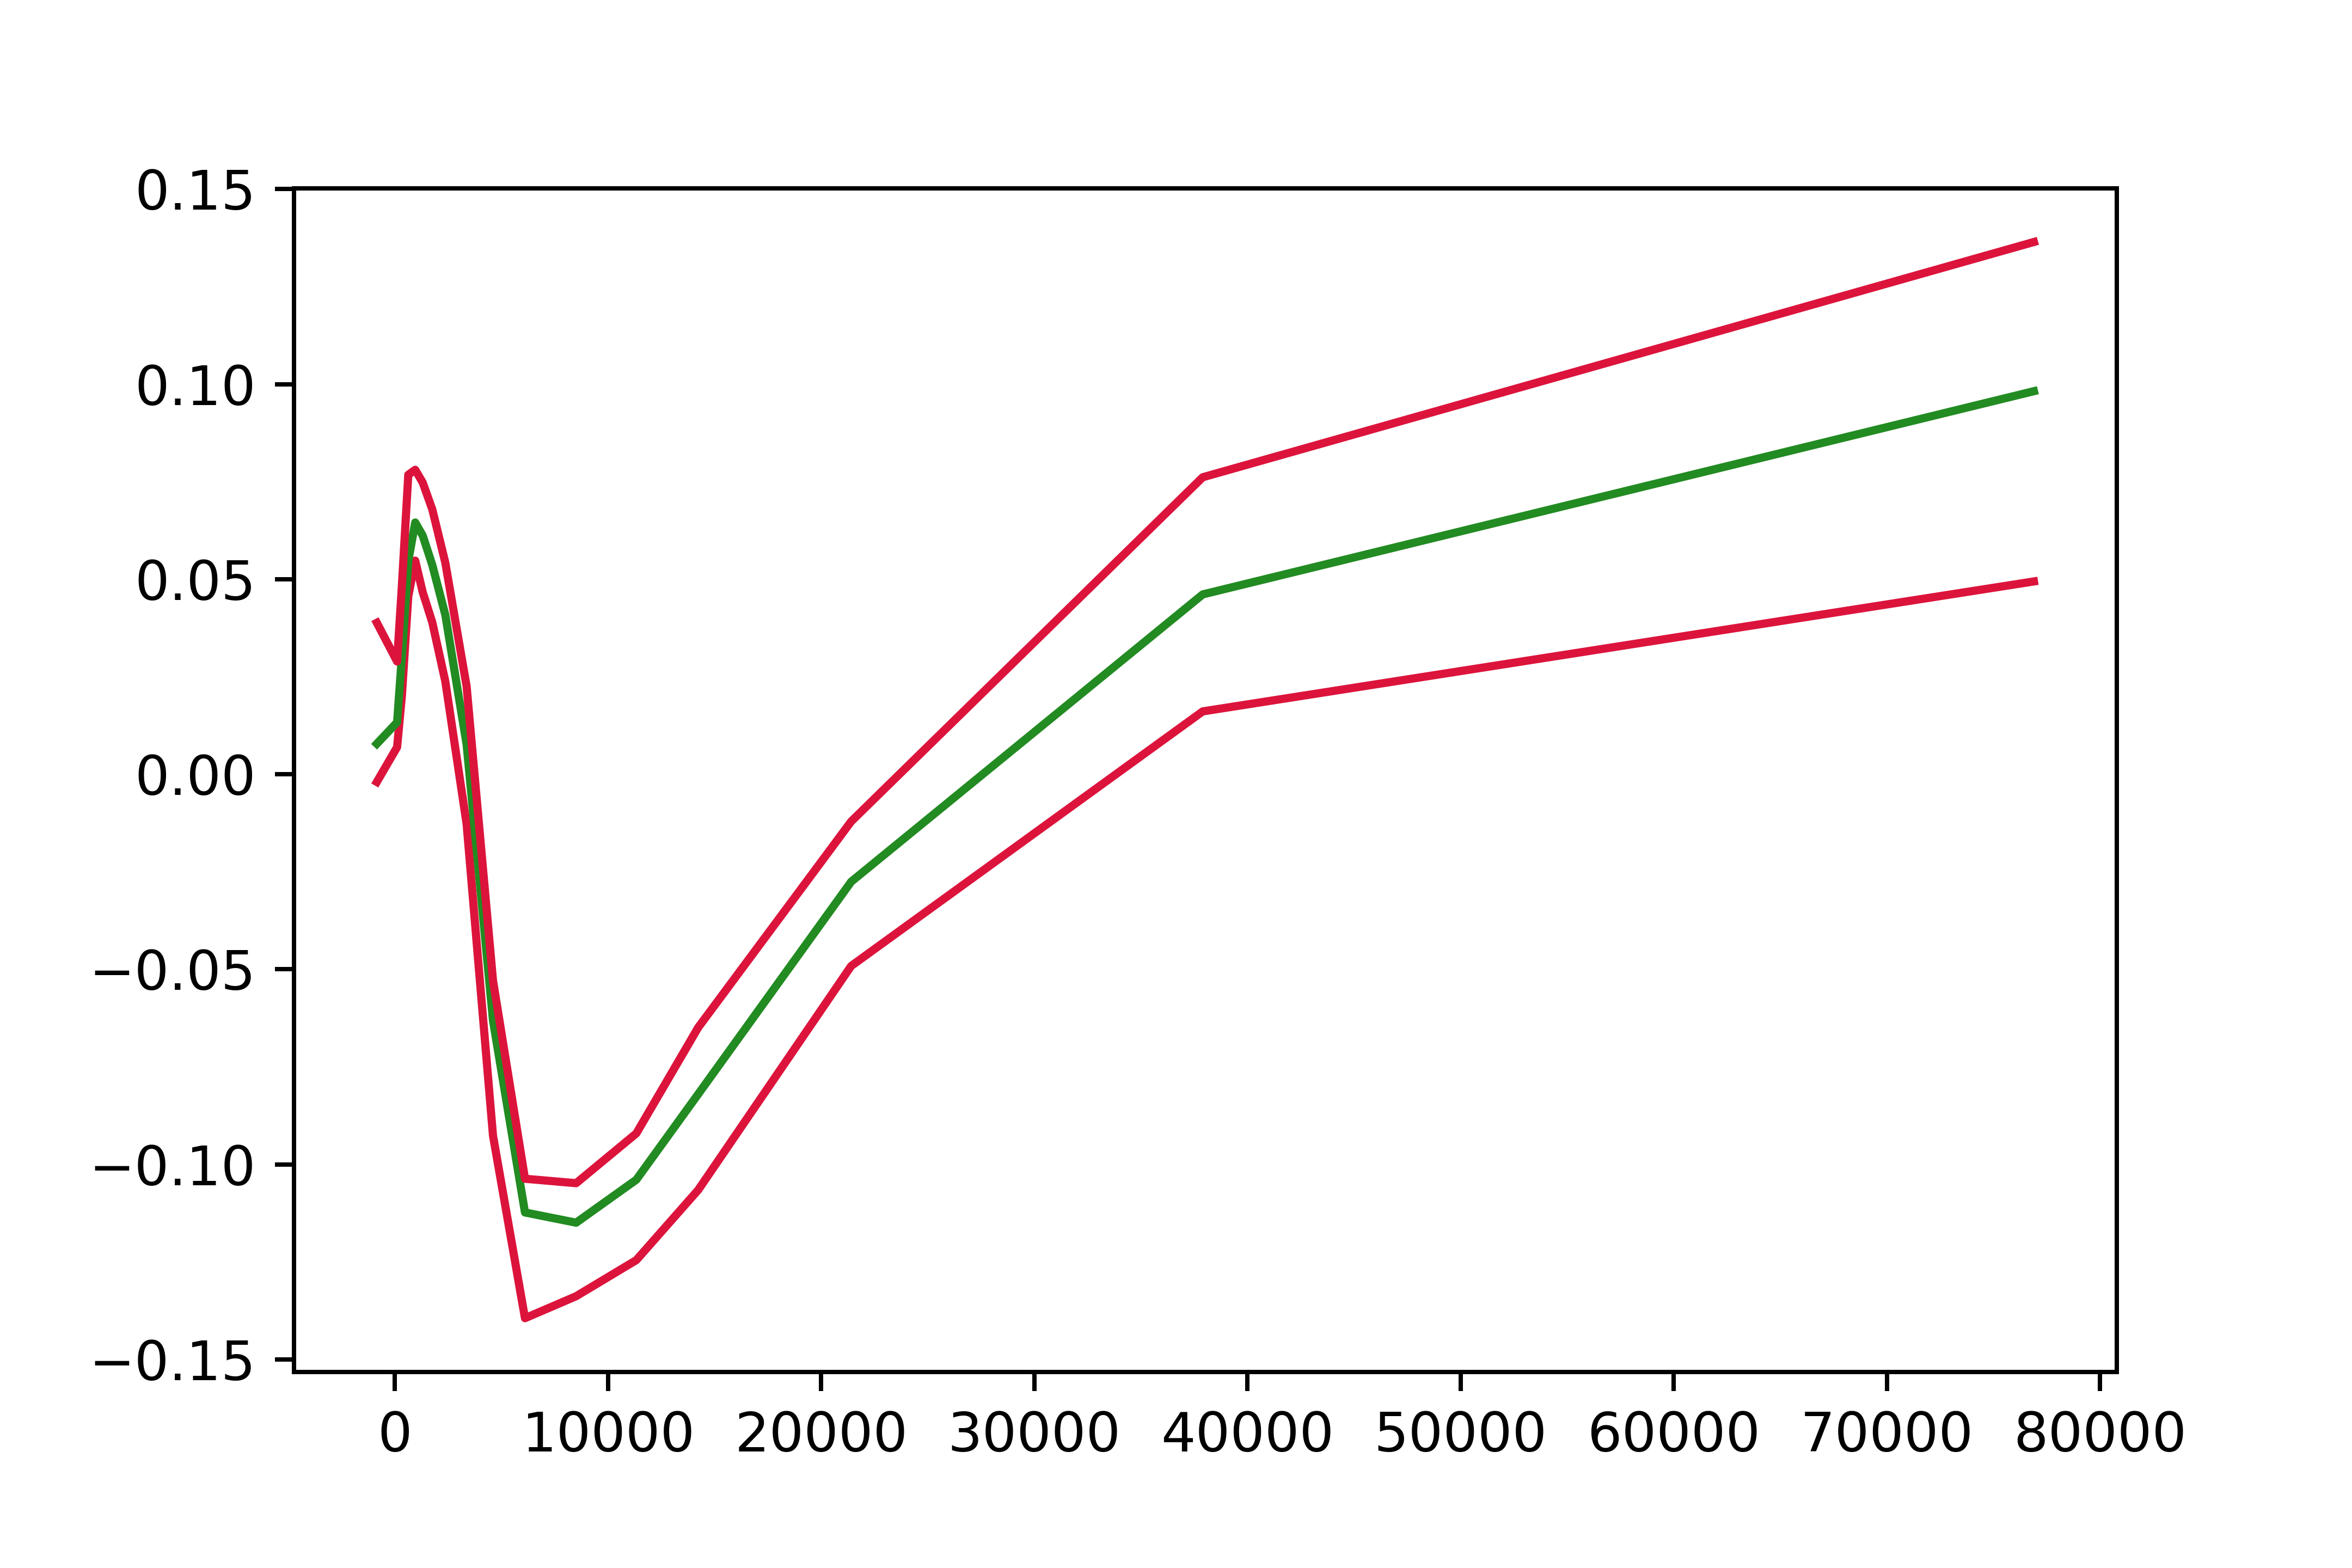
\includegraphics[width=\linewidth]{figures/ALE/chSNDexp/spec3_cf_liqassii.png}
        \caption{Liquid Assets - causal forest}
    \end{subfigure}

    \begin{subfigure}{0.5\linewidth}
        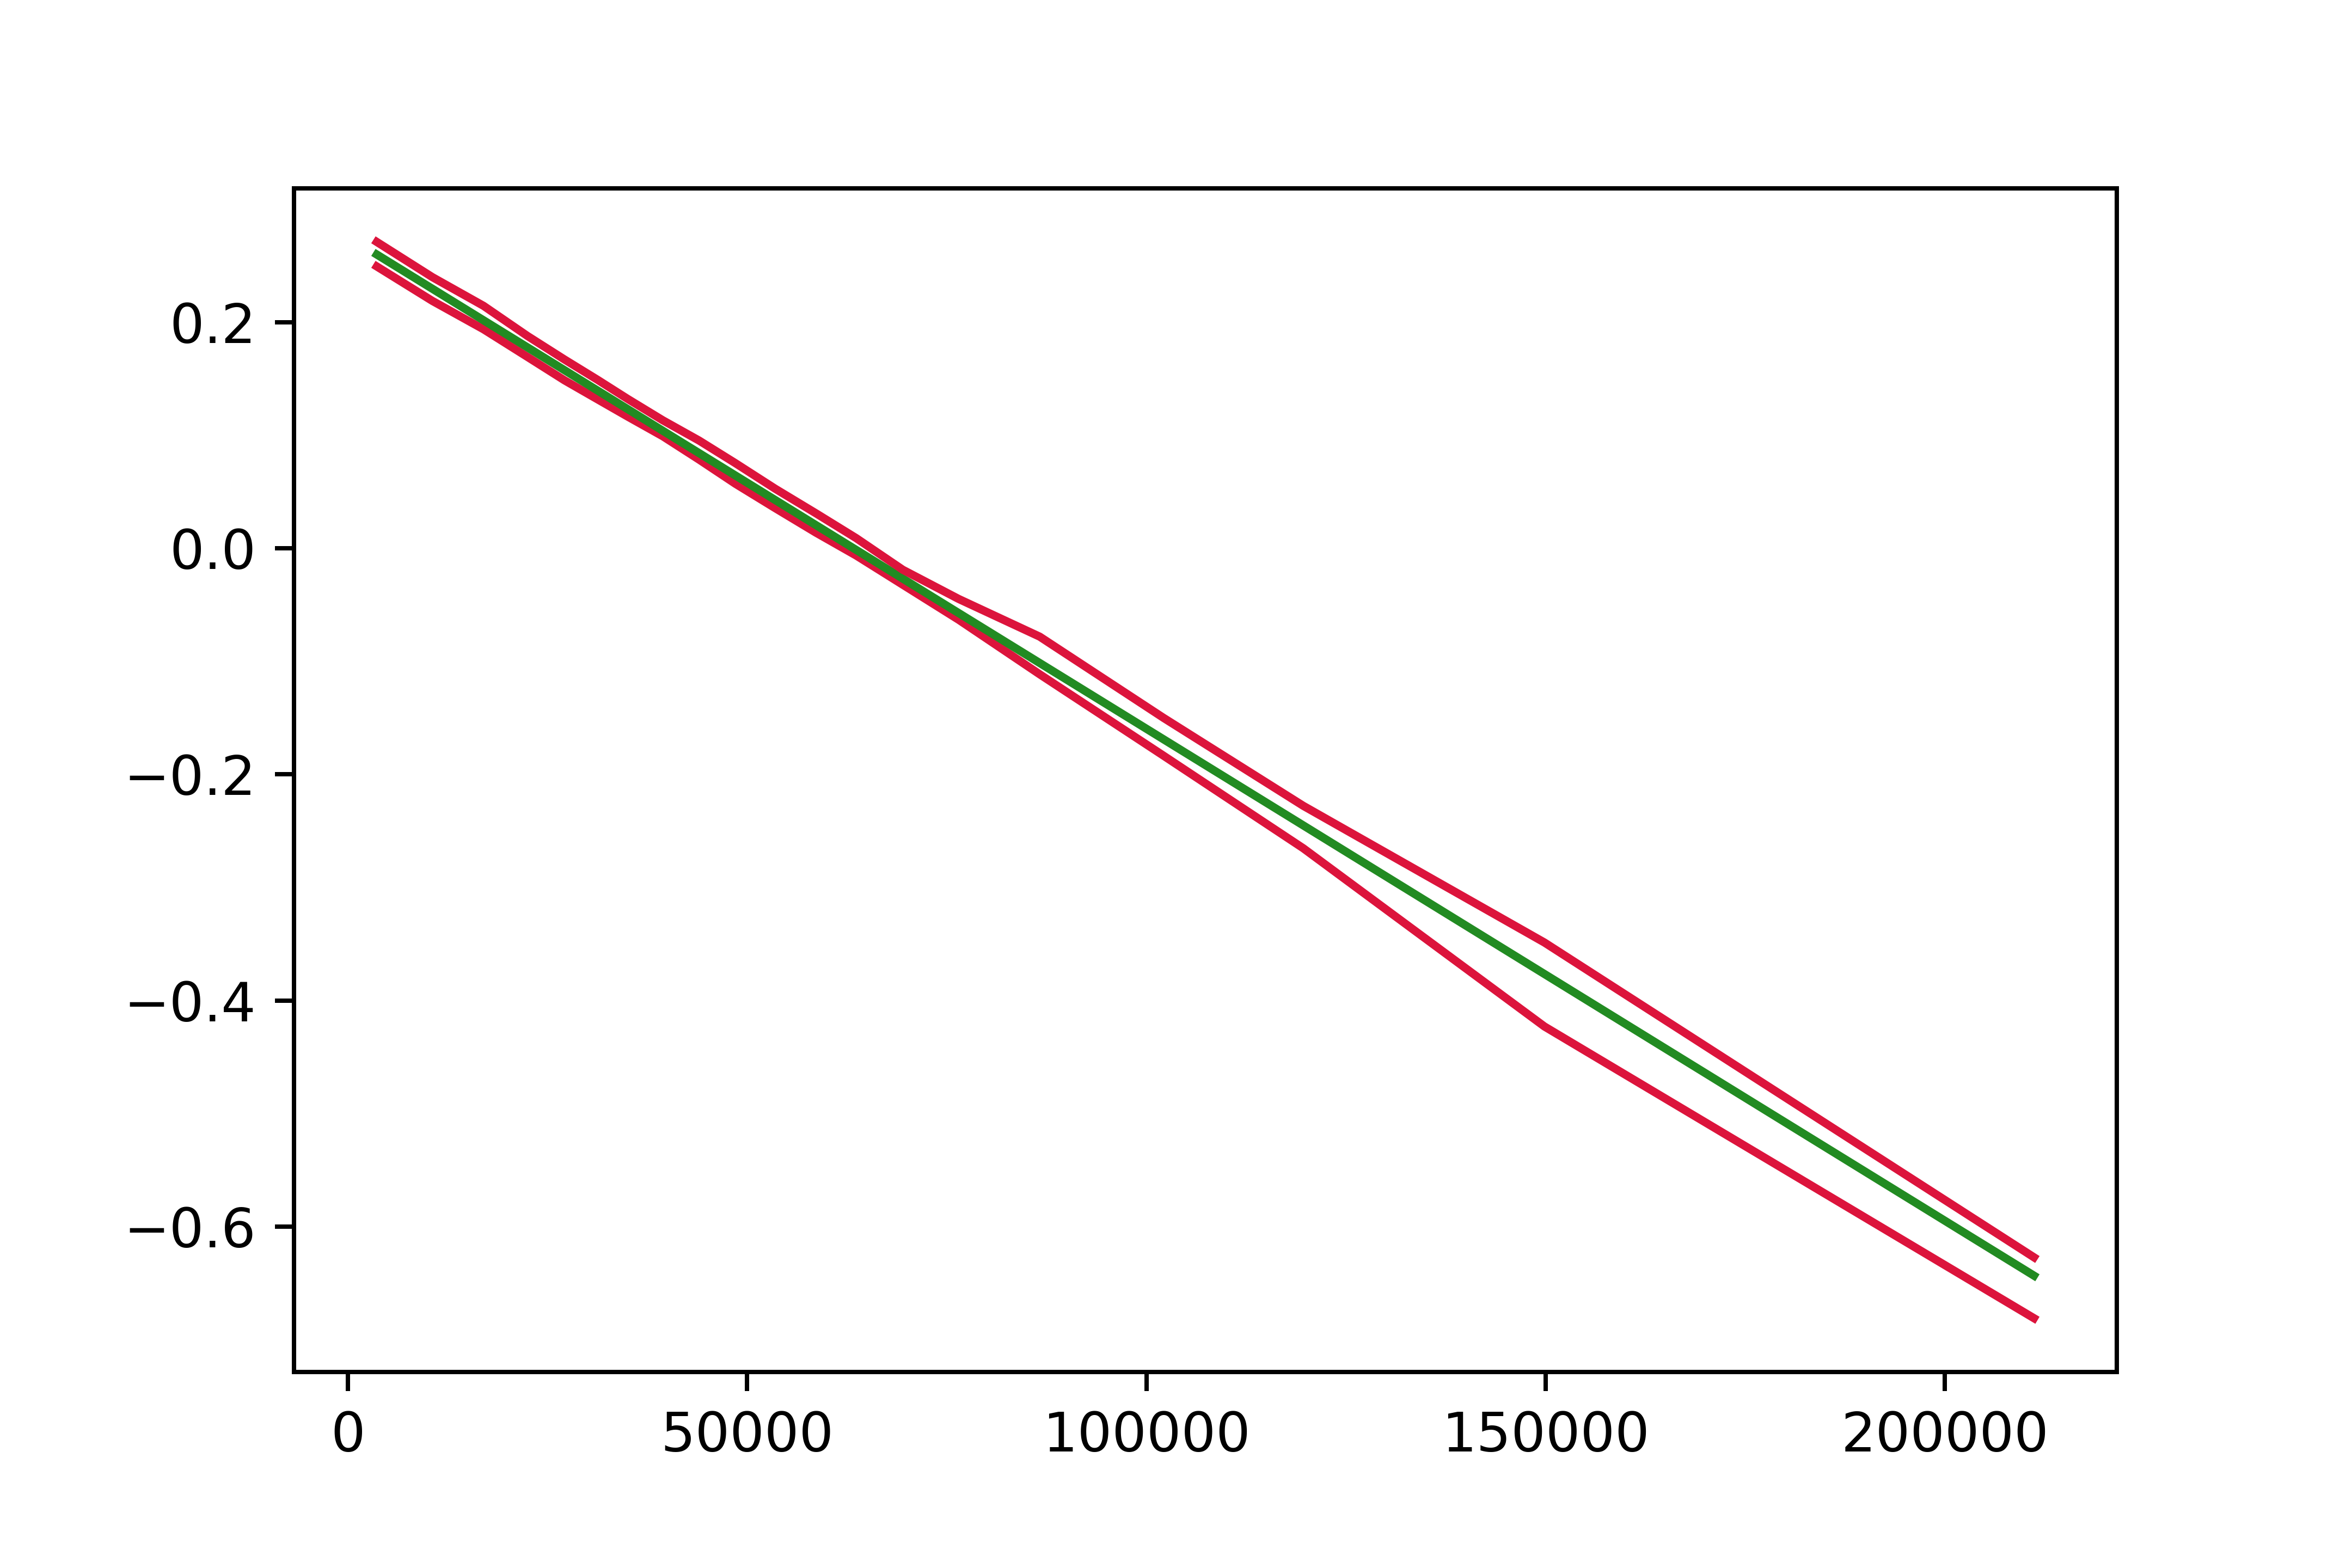
\includegraphics[width=\linewidth]{figures/ALE/chSNDexp/spec3_linear_FSALARYM.png}
        \caption{Salary - linear}
    \end{subfigure}%
    \begin{subfigure}{0.5\linewidth}
        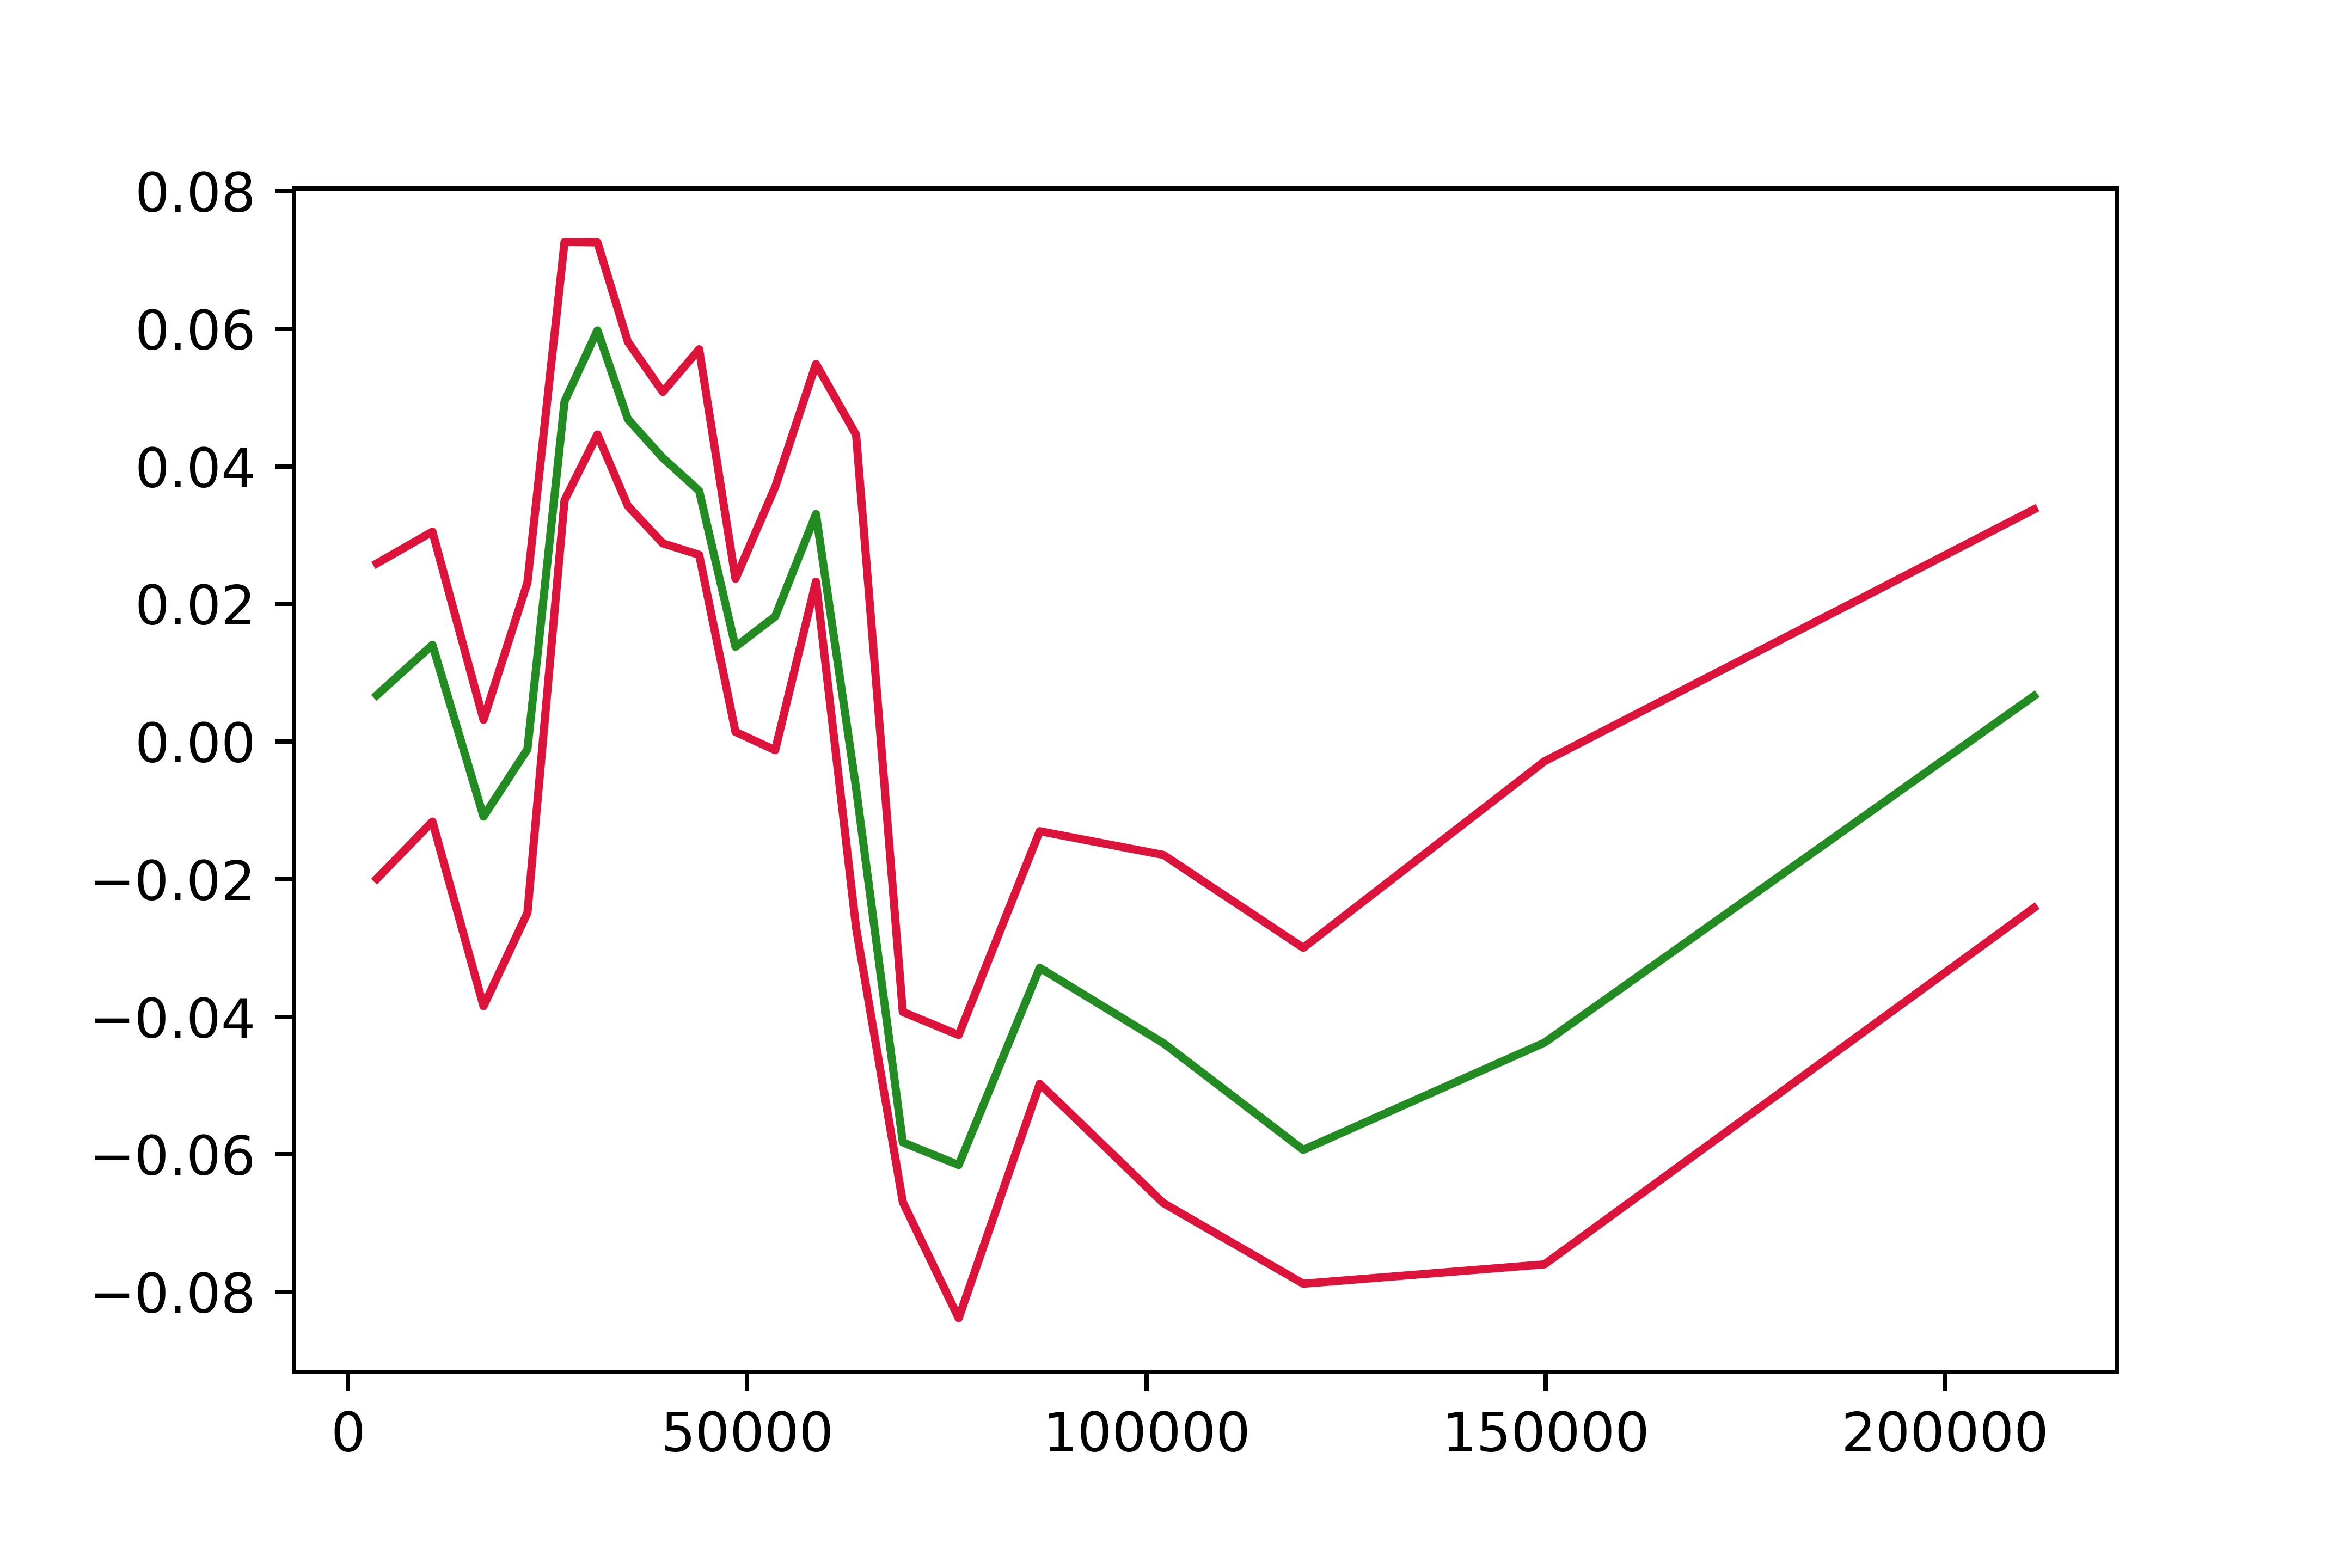
\includegraphics[width=\linewidth]{figures/ALE/chSNDexp/spec3_cf_FSALARYM.png}
        \caption{Salary - causal forest}
    \end{subfigure}

    \begin{subfigure}{0.5\linewidth}
        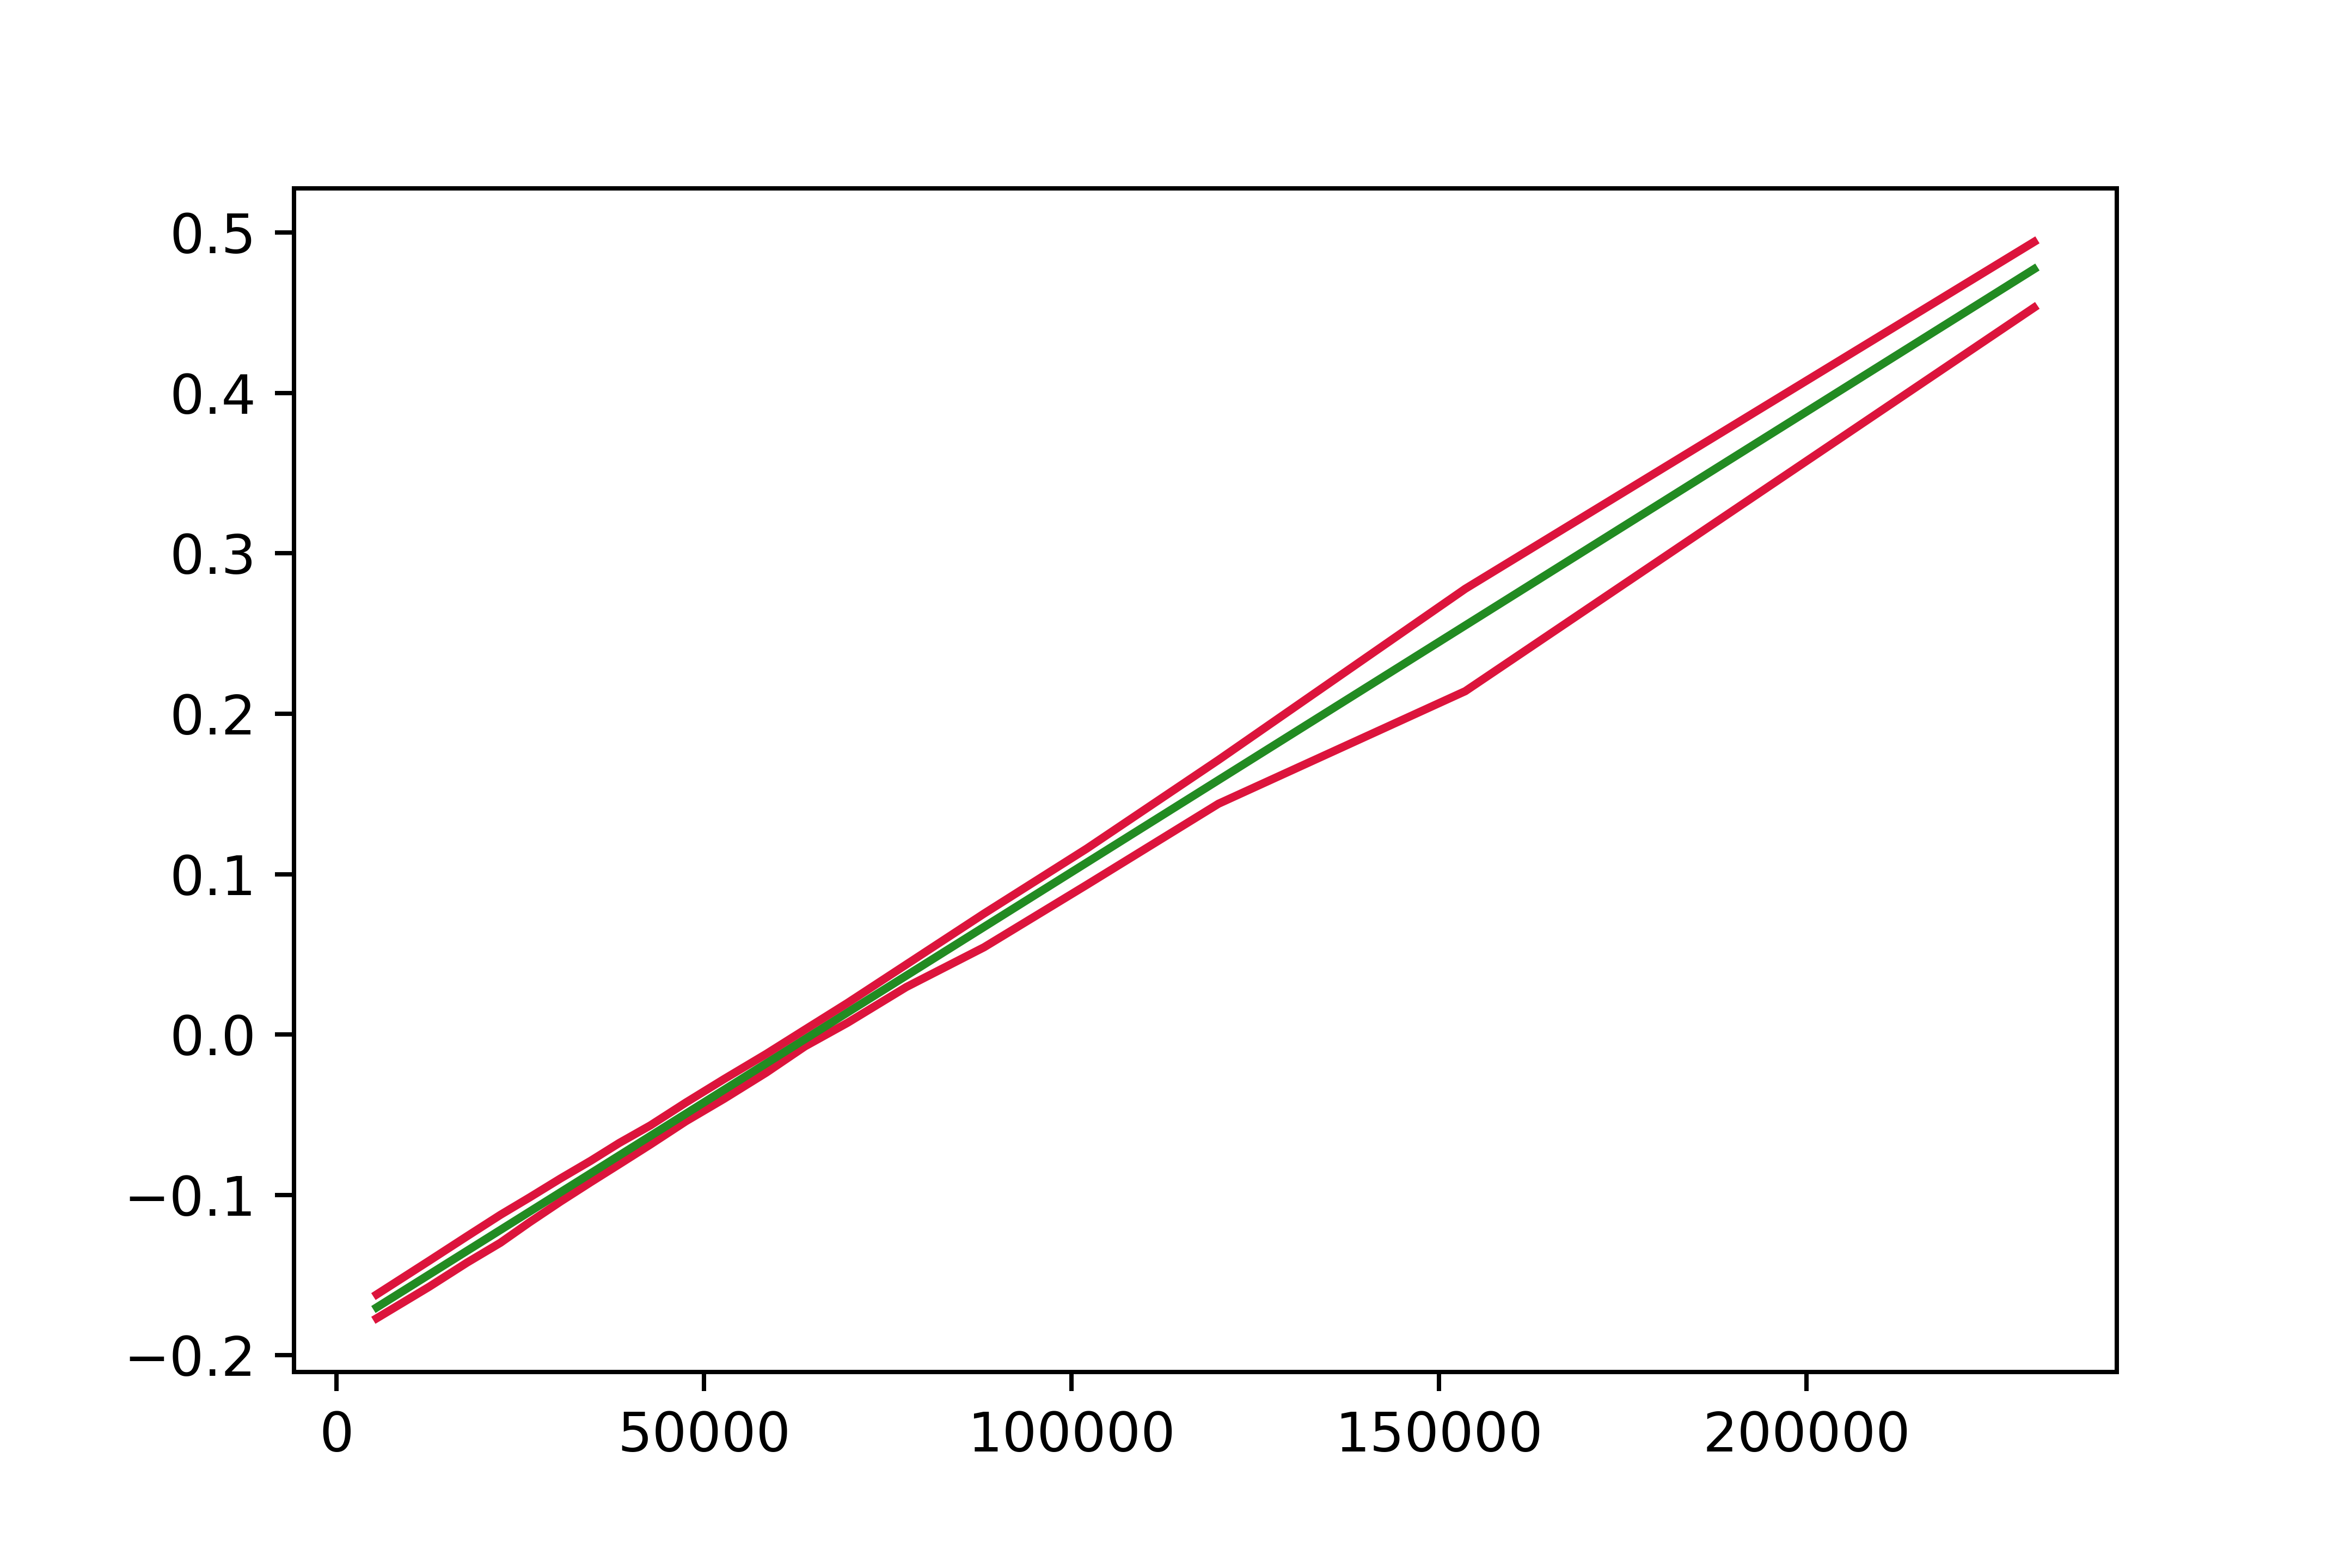
\includegraphics[width=\linewidth]{figures/ALE/chSNDexp/spec3_linear_FINCBTXM.png}
        \caption{Income - linear}
    \end{subfigure}%
    \begin{subfigure}{0.5\linewidth}
        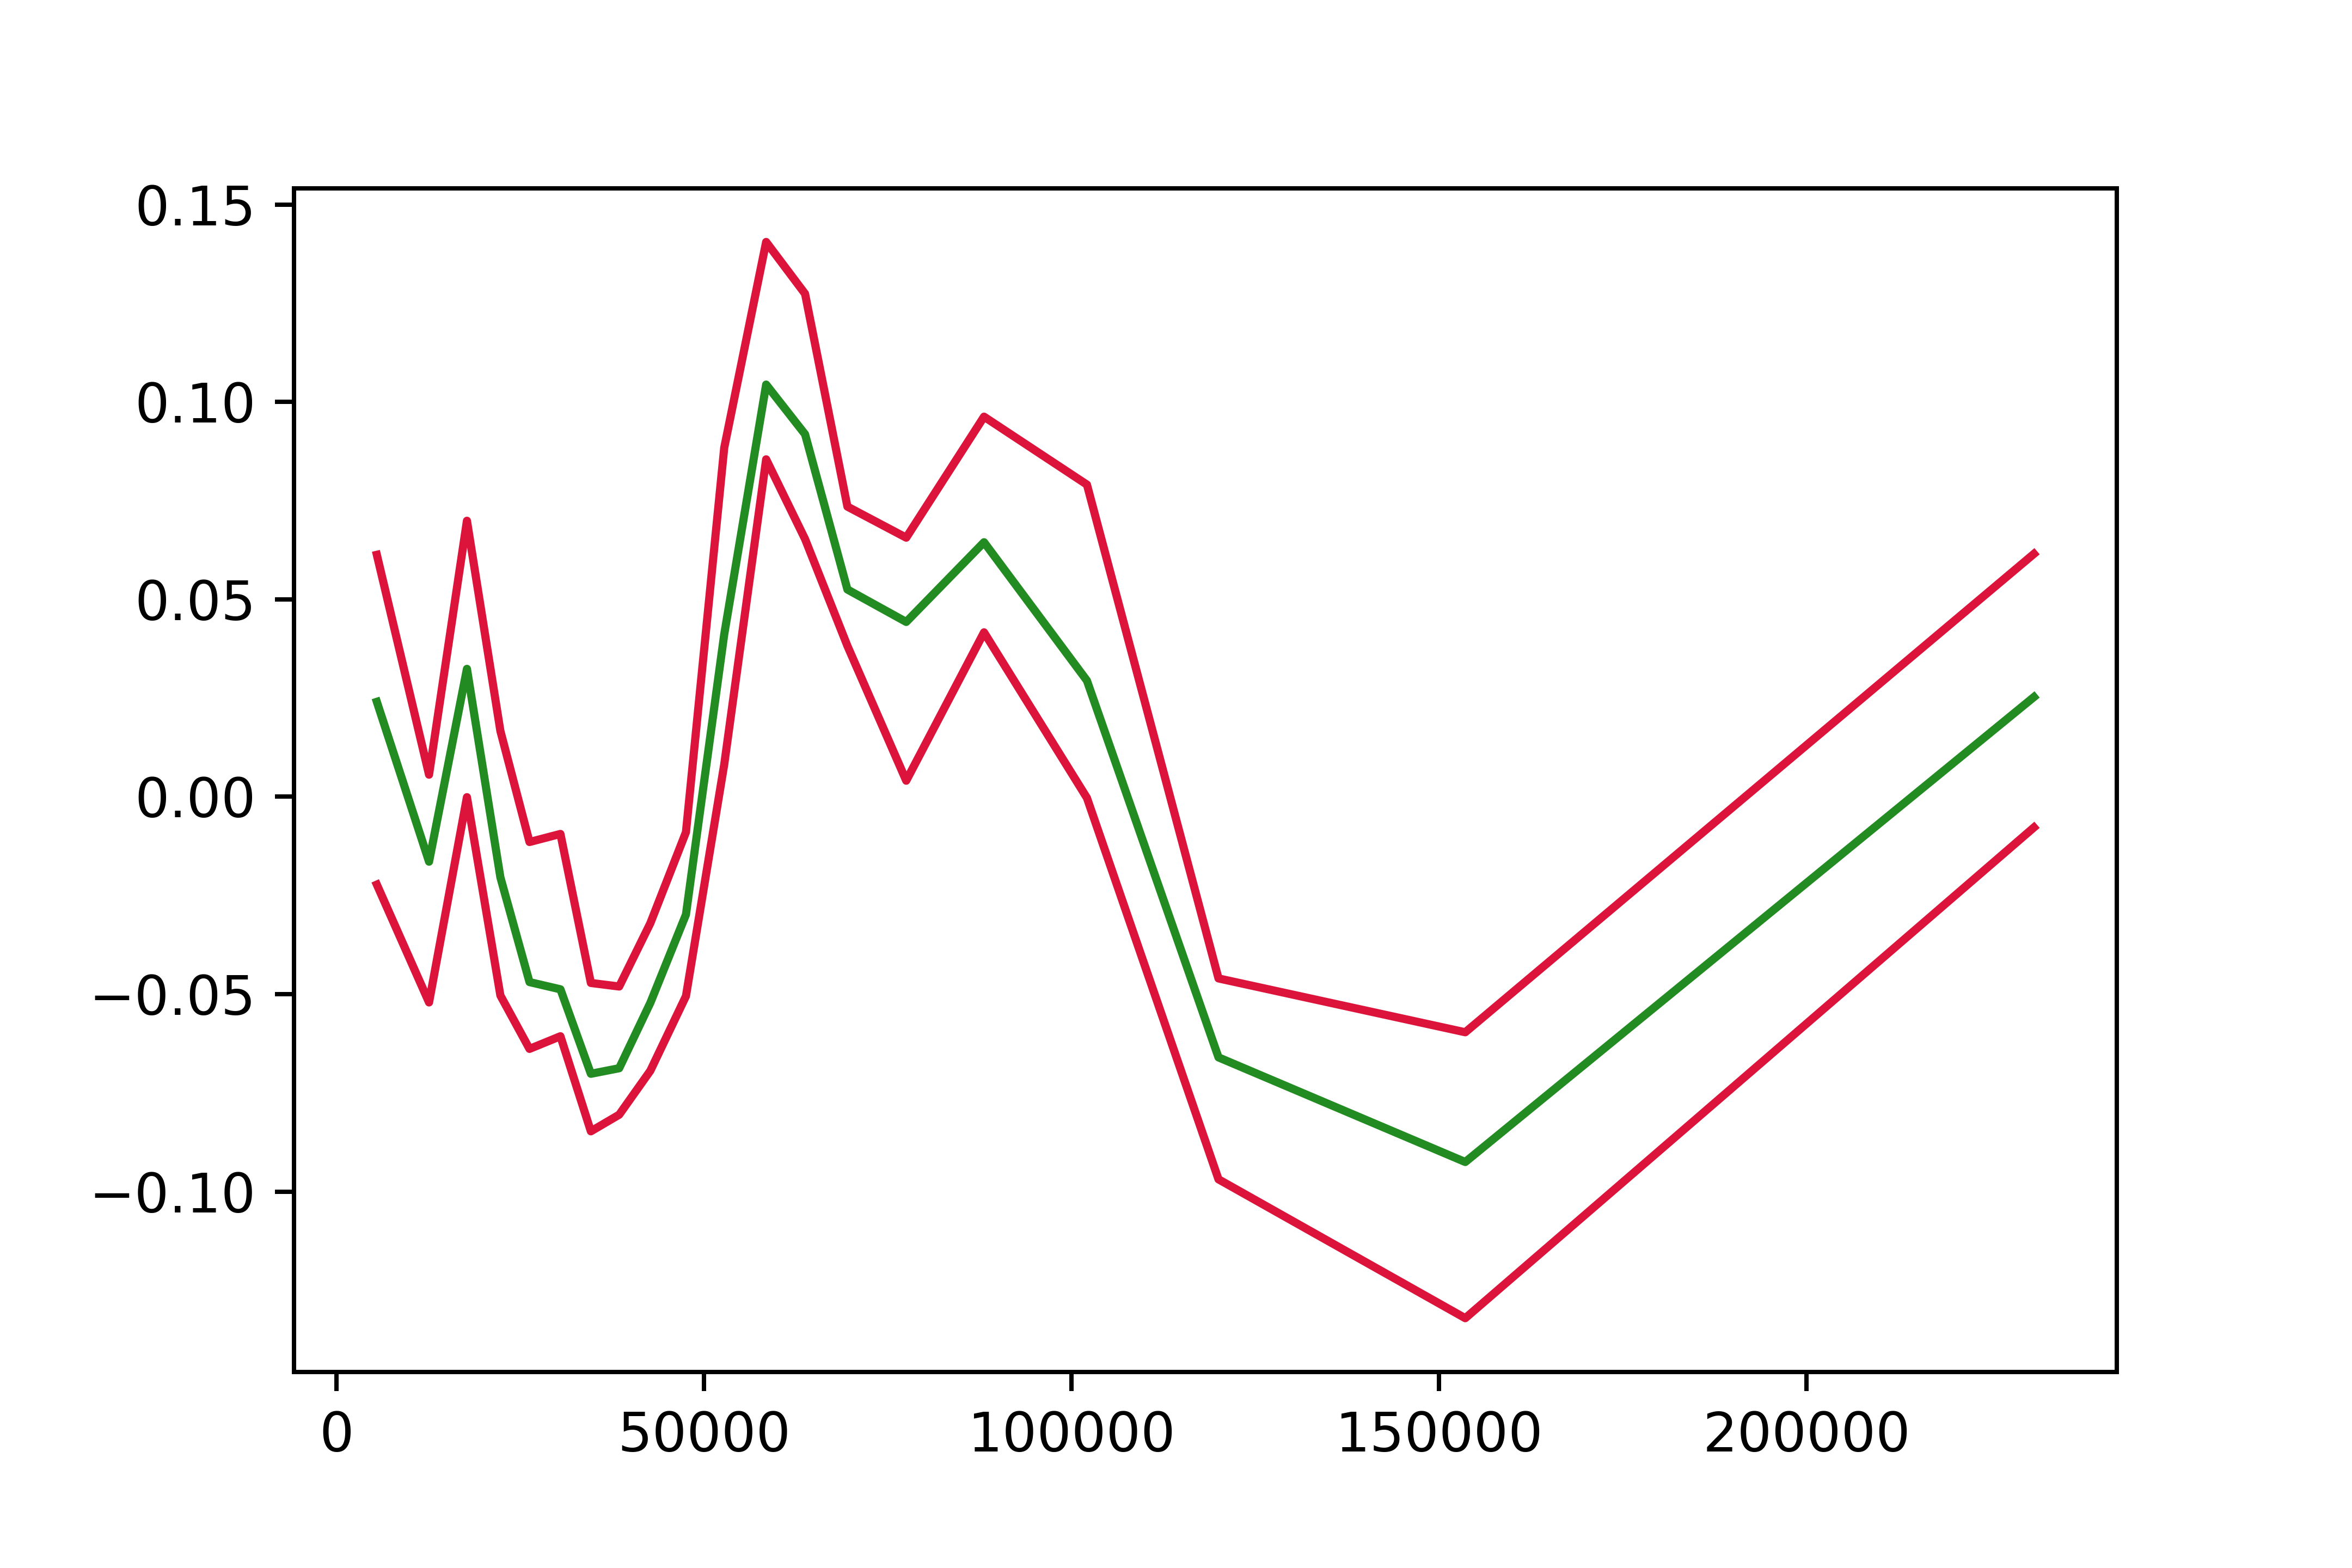
\includegraphics[width=\linewidth]{figures/ALE/chSNDexp/spec3_cf_FINCBTXM.png}
        \caption{Income - causal forest}
    \end{subfigure}
    \caption{ALE of \textit{financial status} variables - total expenditures}
    \label{app:ale_finstat_snd}
\end{figure}

%! FD - Age
\begin{figure}[h]
    \centering
    \begin{subfigure}{0.5\linewidth}
        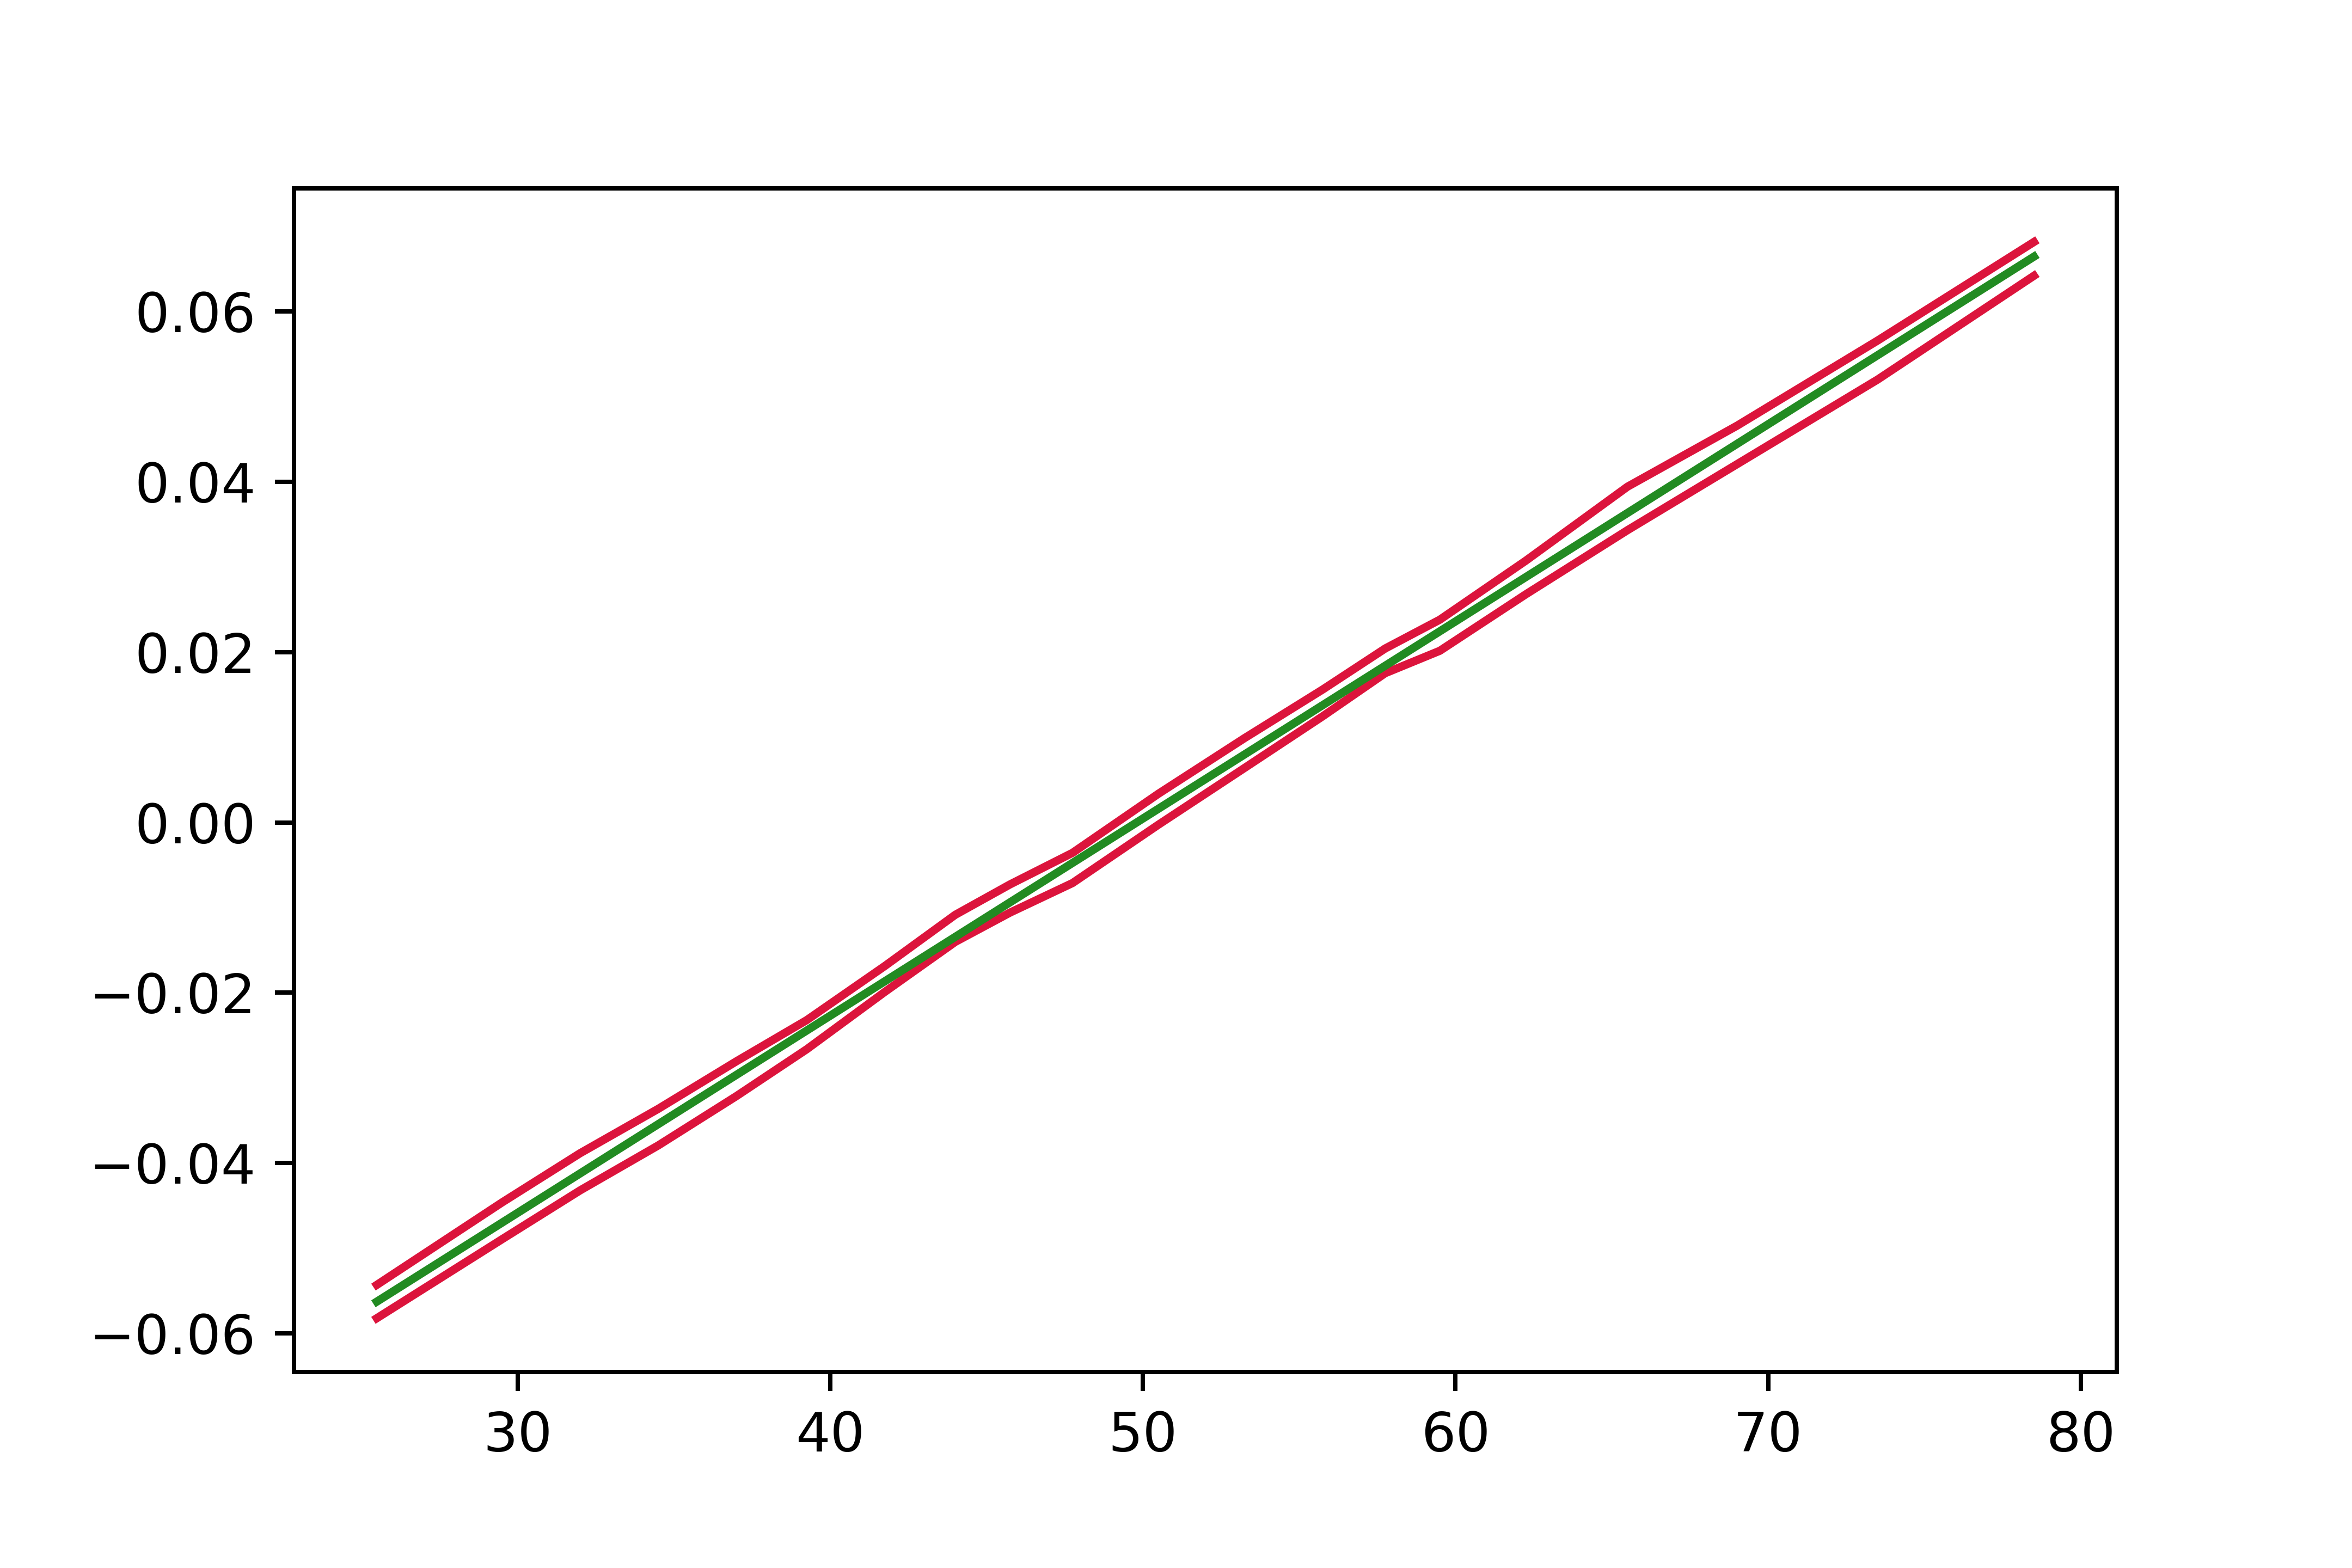
\includegraphics[width=\linewidth]{figures/ALE/chFDexp/spec1_linear_AGE.png}
        \caption{Spec 1 - linear}
    \end{subfigure}%
    \begin{subfigure}{0.5\linewidth}
        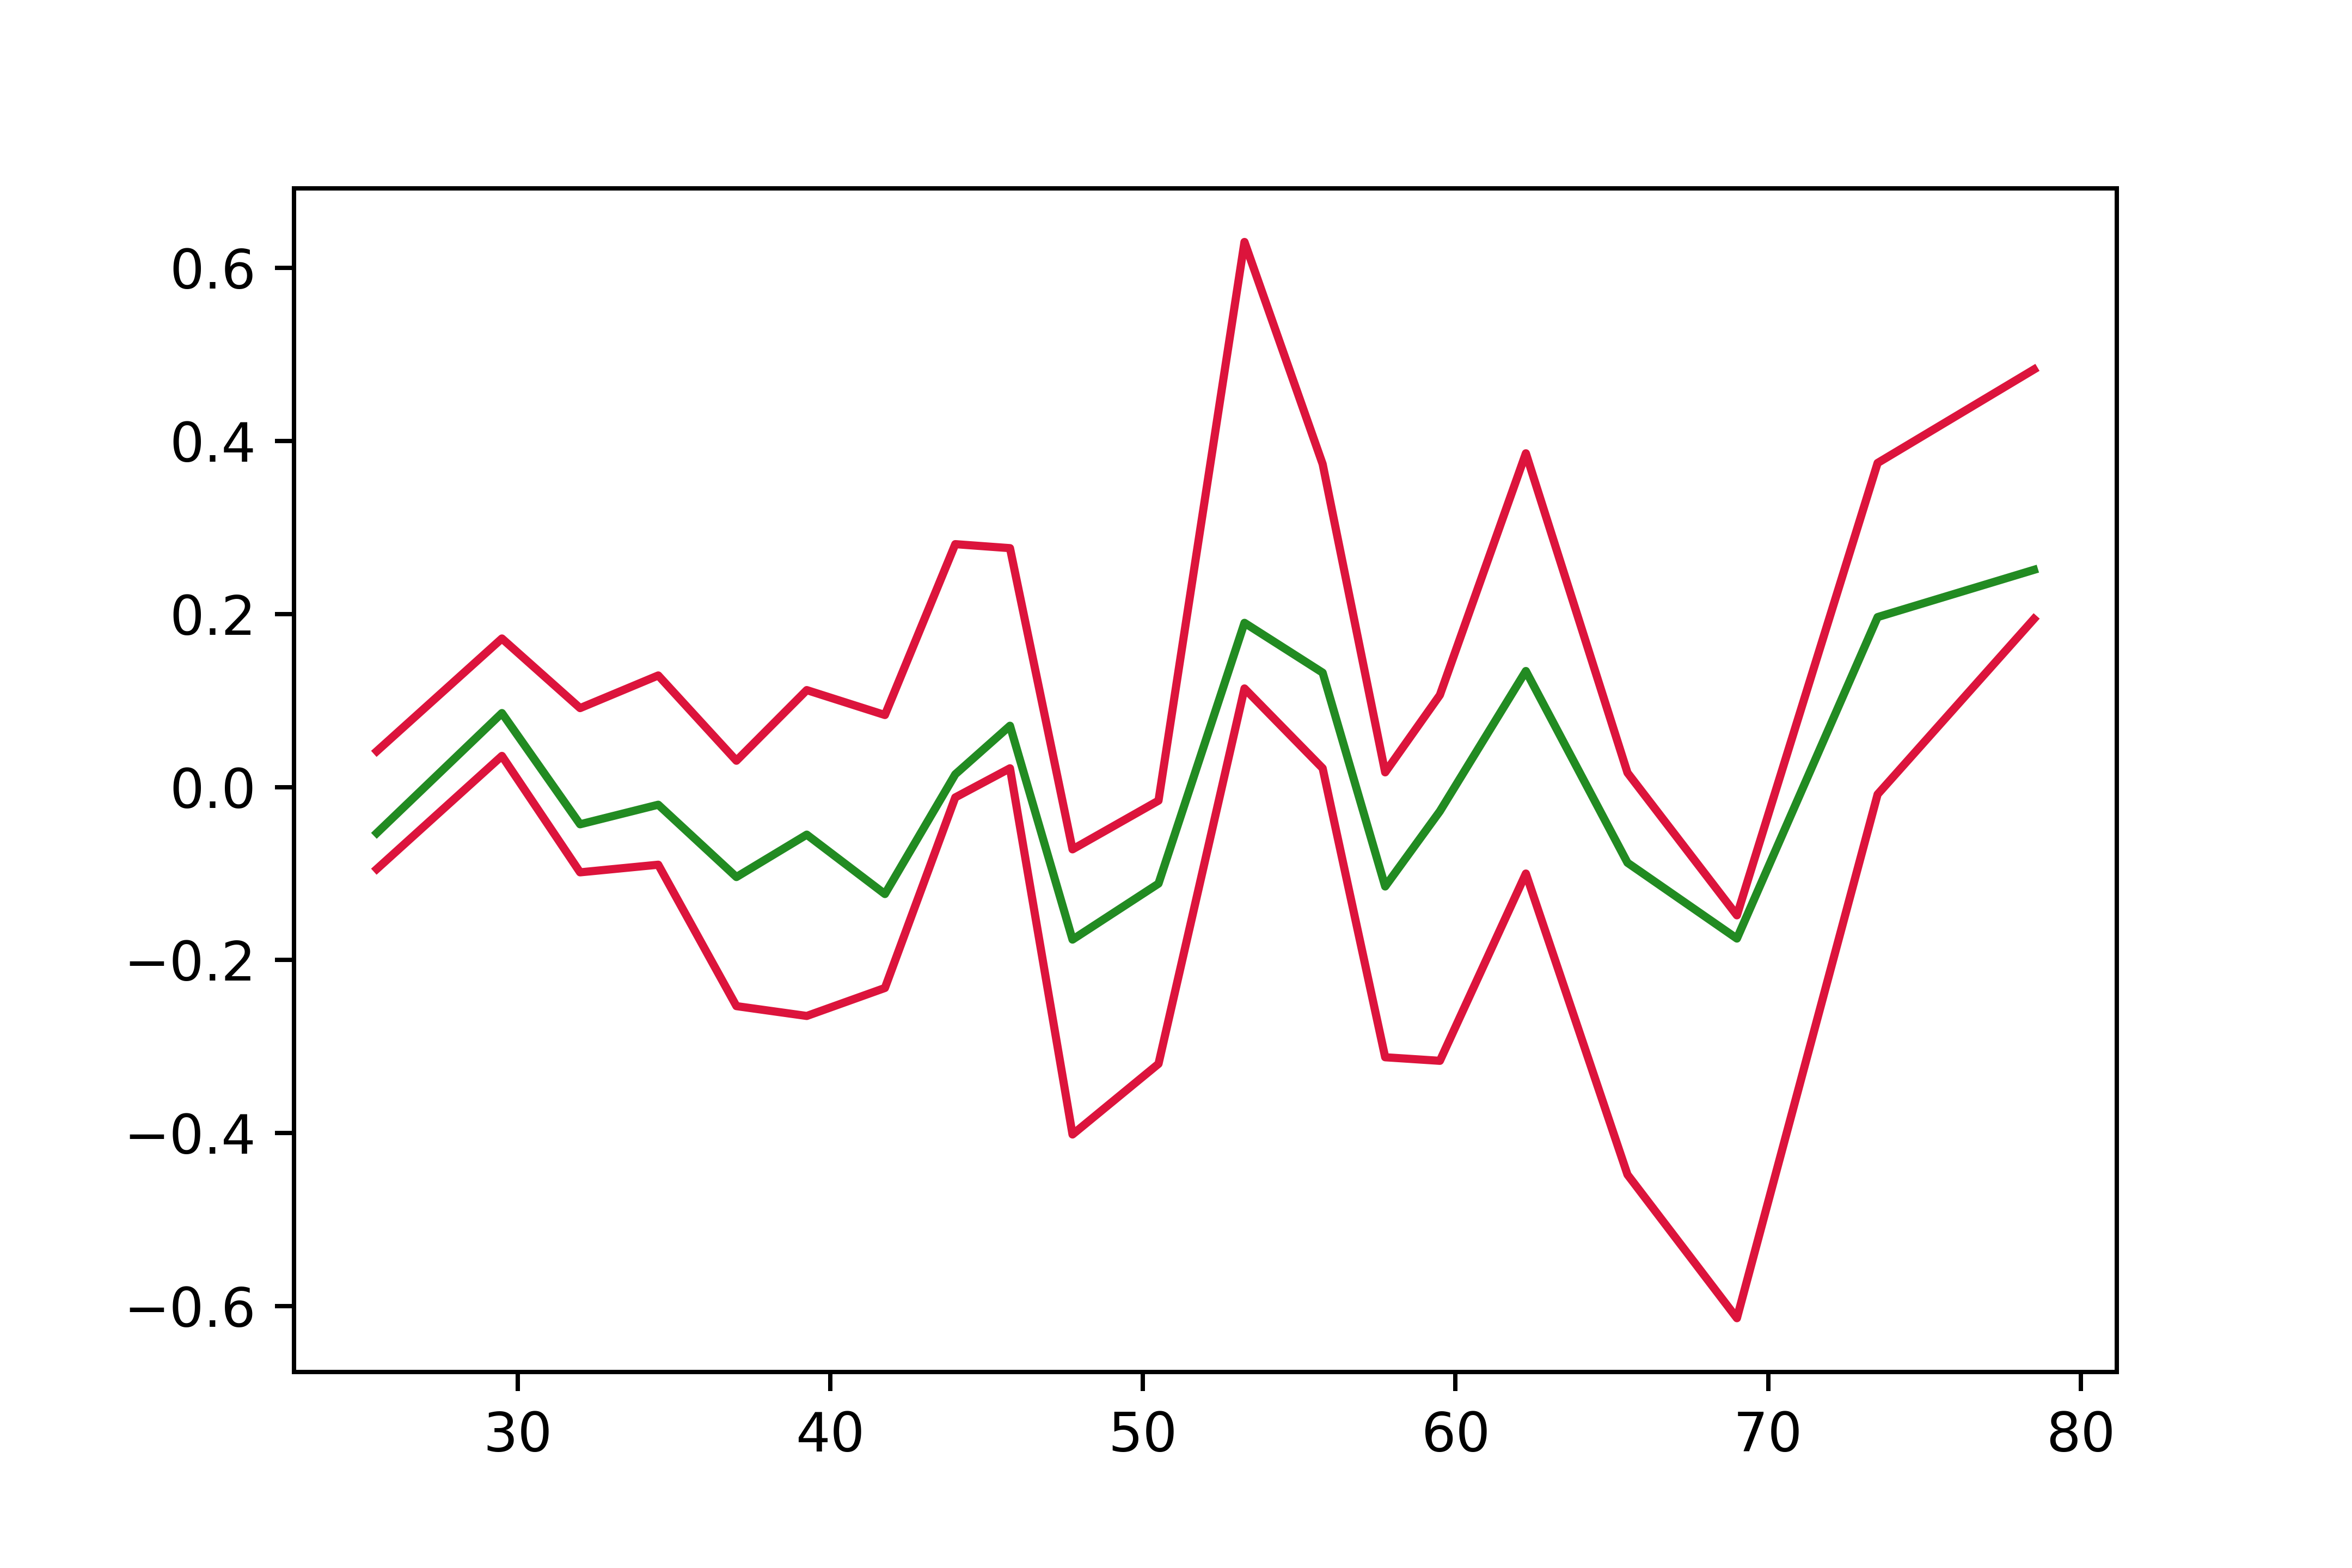
\includegraphics[width=\linewidth]{figures/ALE/chFDexp/spec1_cf_AGE.png}
        \caption{Spec 1 - causal forest}
    \end{subfigure}

    \begin{subfigure}{0.5\linewidth}
        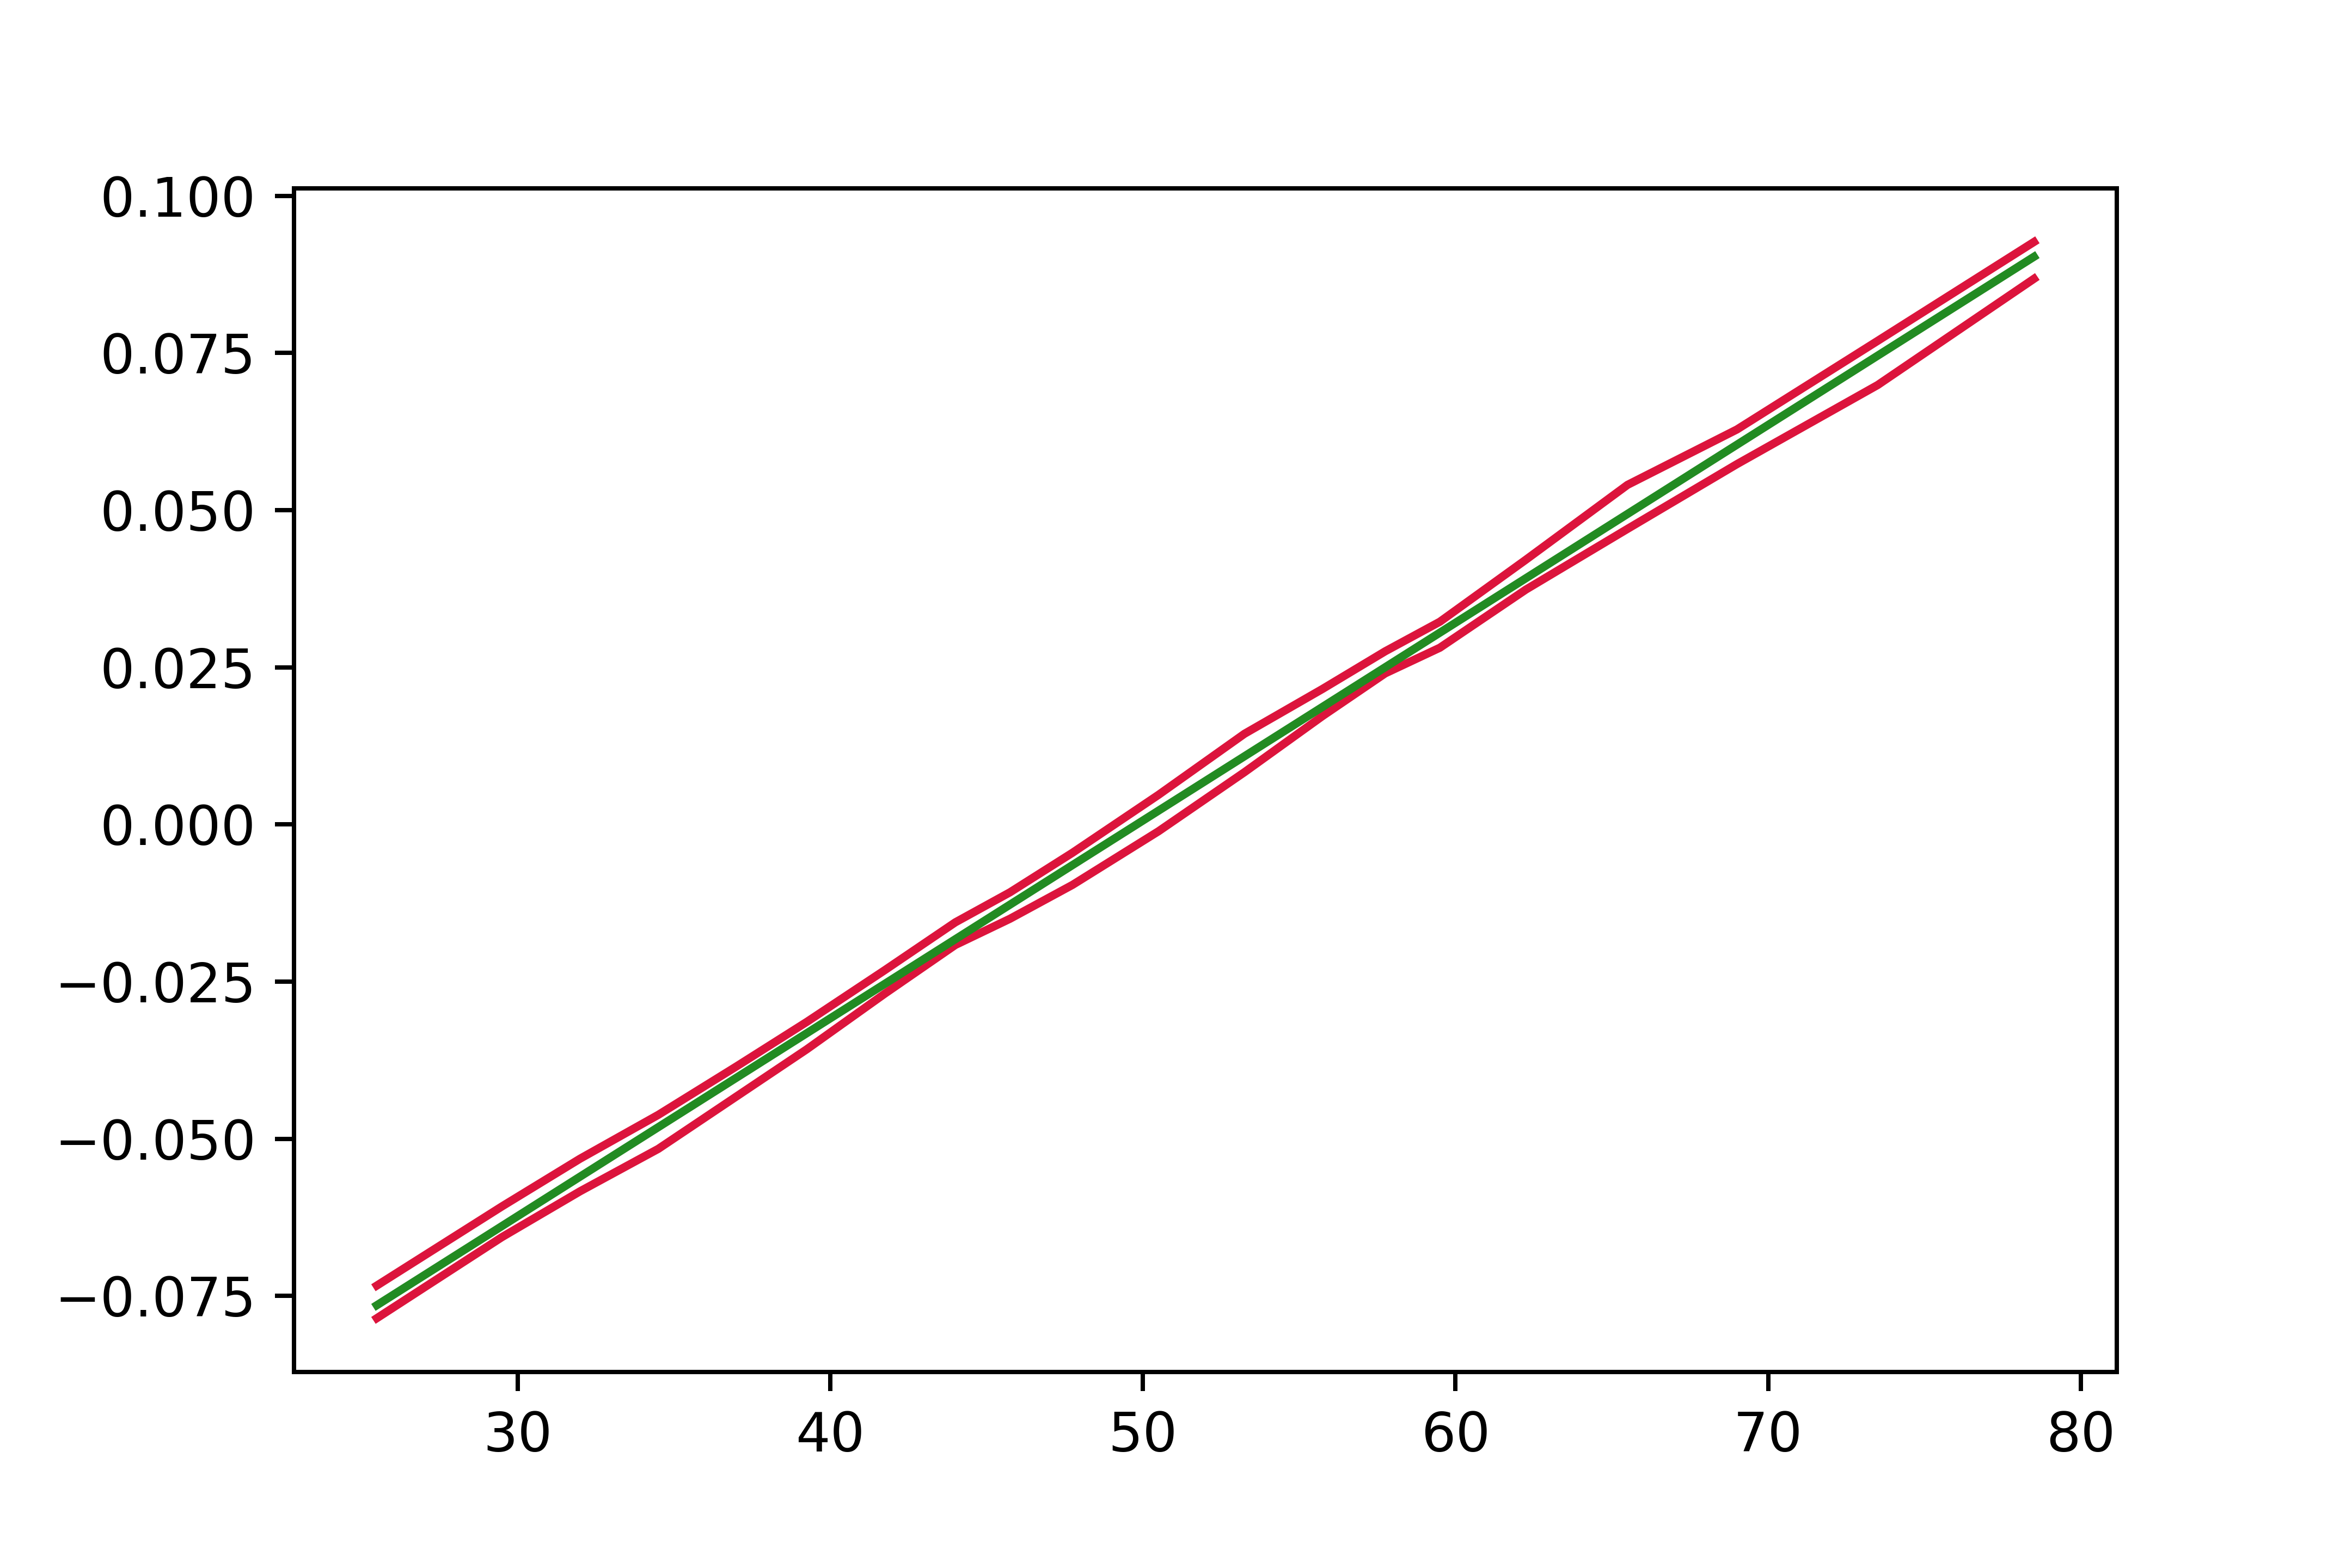
\includegraphics[width=\linewidth]{figures/ALE/chFDexp/spec2_linear_AGE.png}
        \caption{Spec 2 - linear}
    \end{subfigure}%
    \begin{subfigure}{0.5\linewidth}
        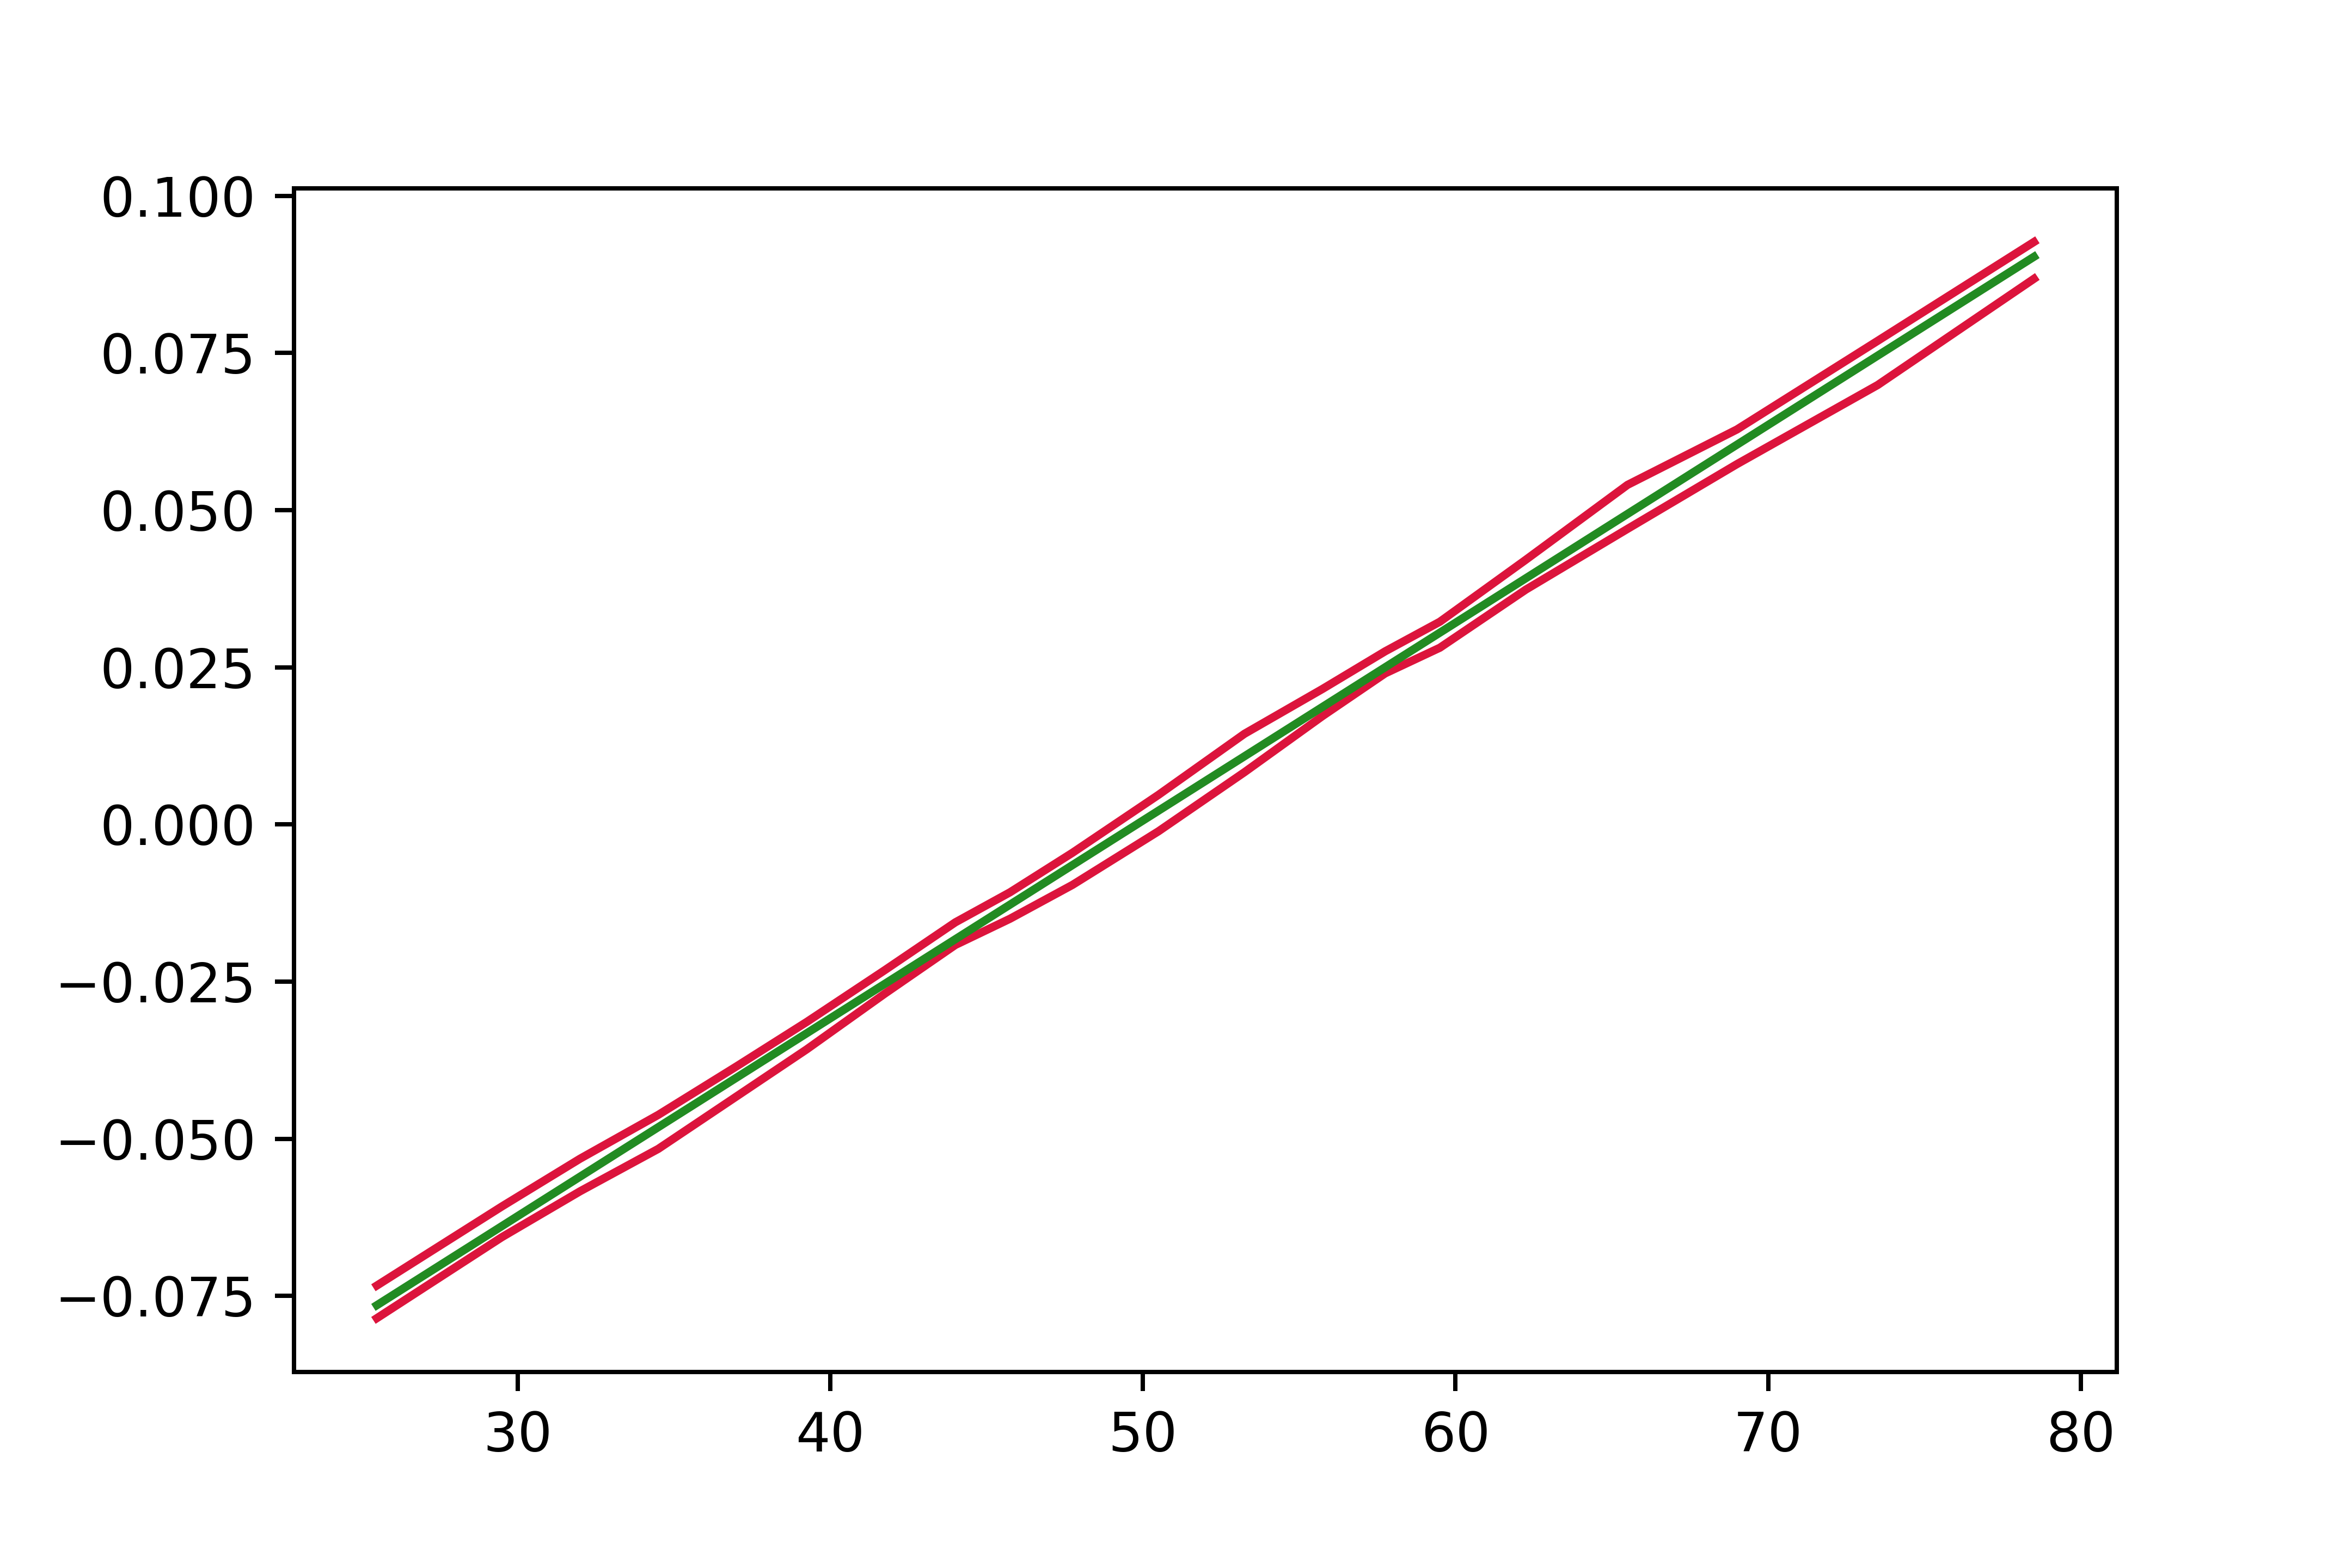
\includegraphics[width=\linewidth]{figures/ALE/chFDexp/spec2_linear_AGE.png}
        \caption{Spec 2 - causal forest}
    \end{subfigure}

    \begin{subfigure}{0.5\linewidth}
        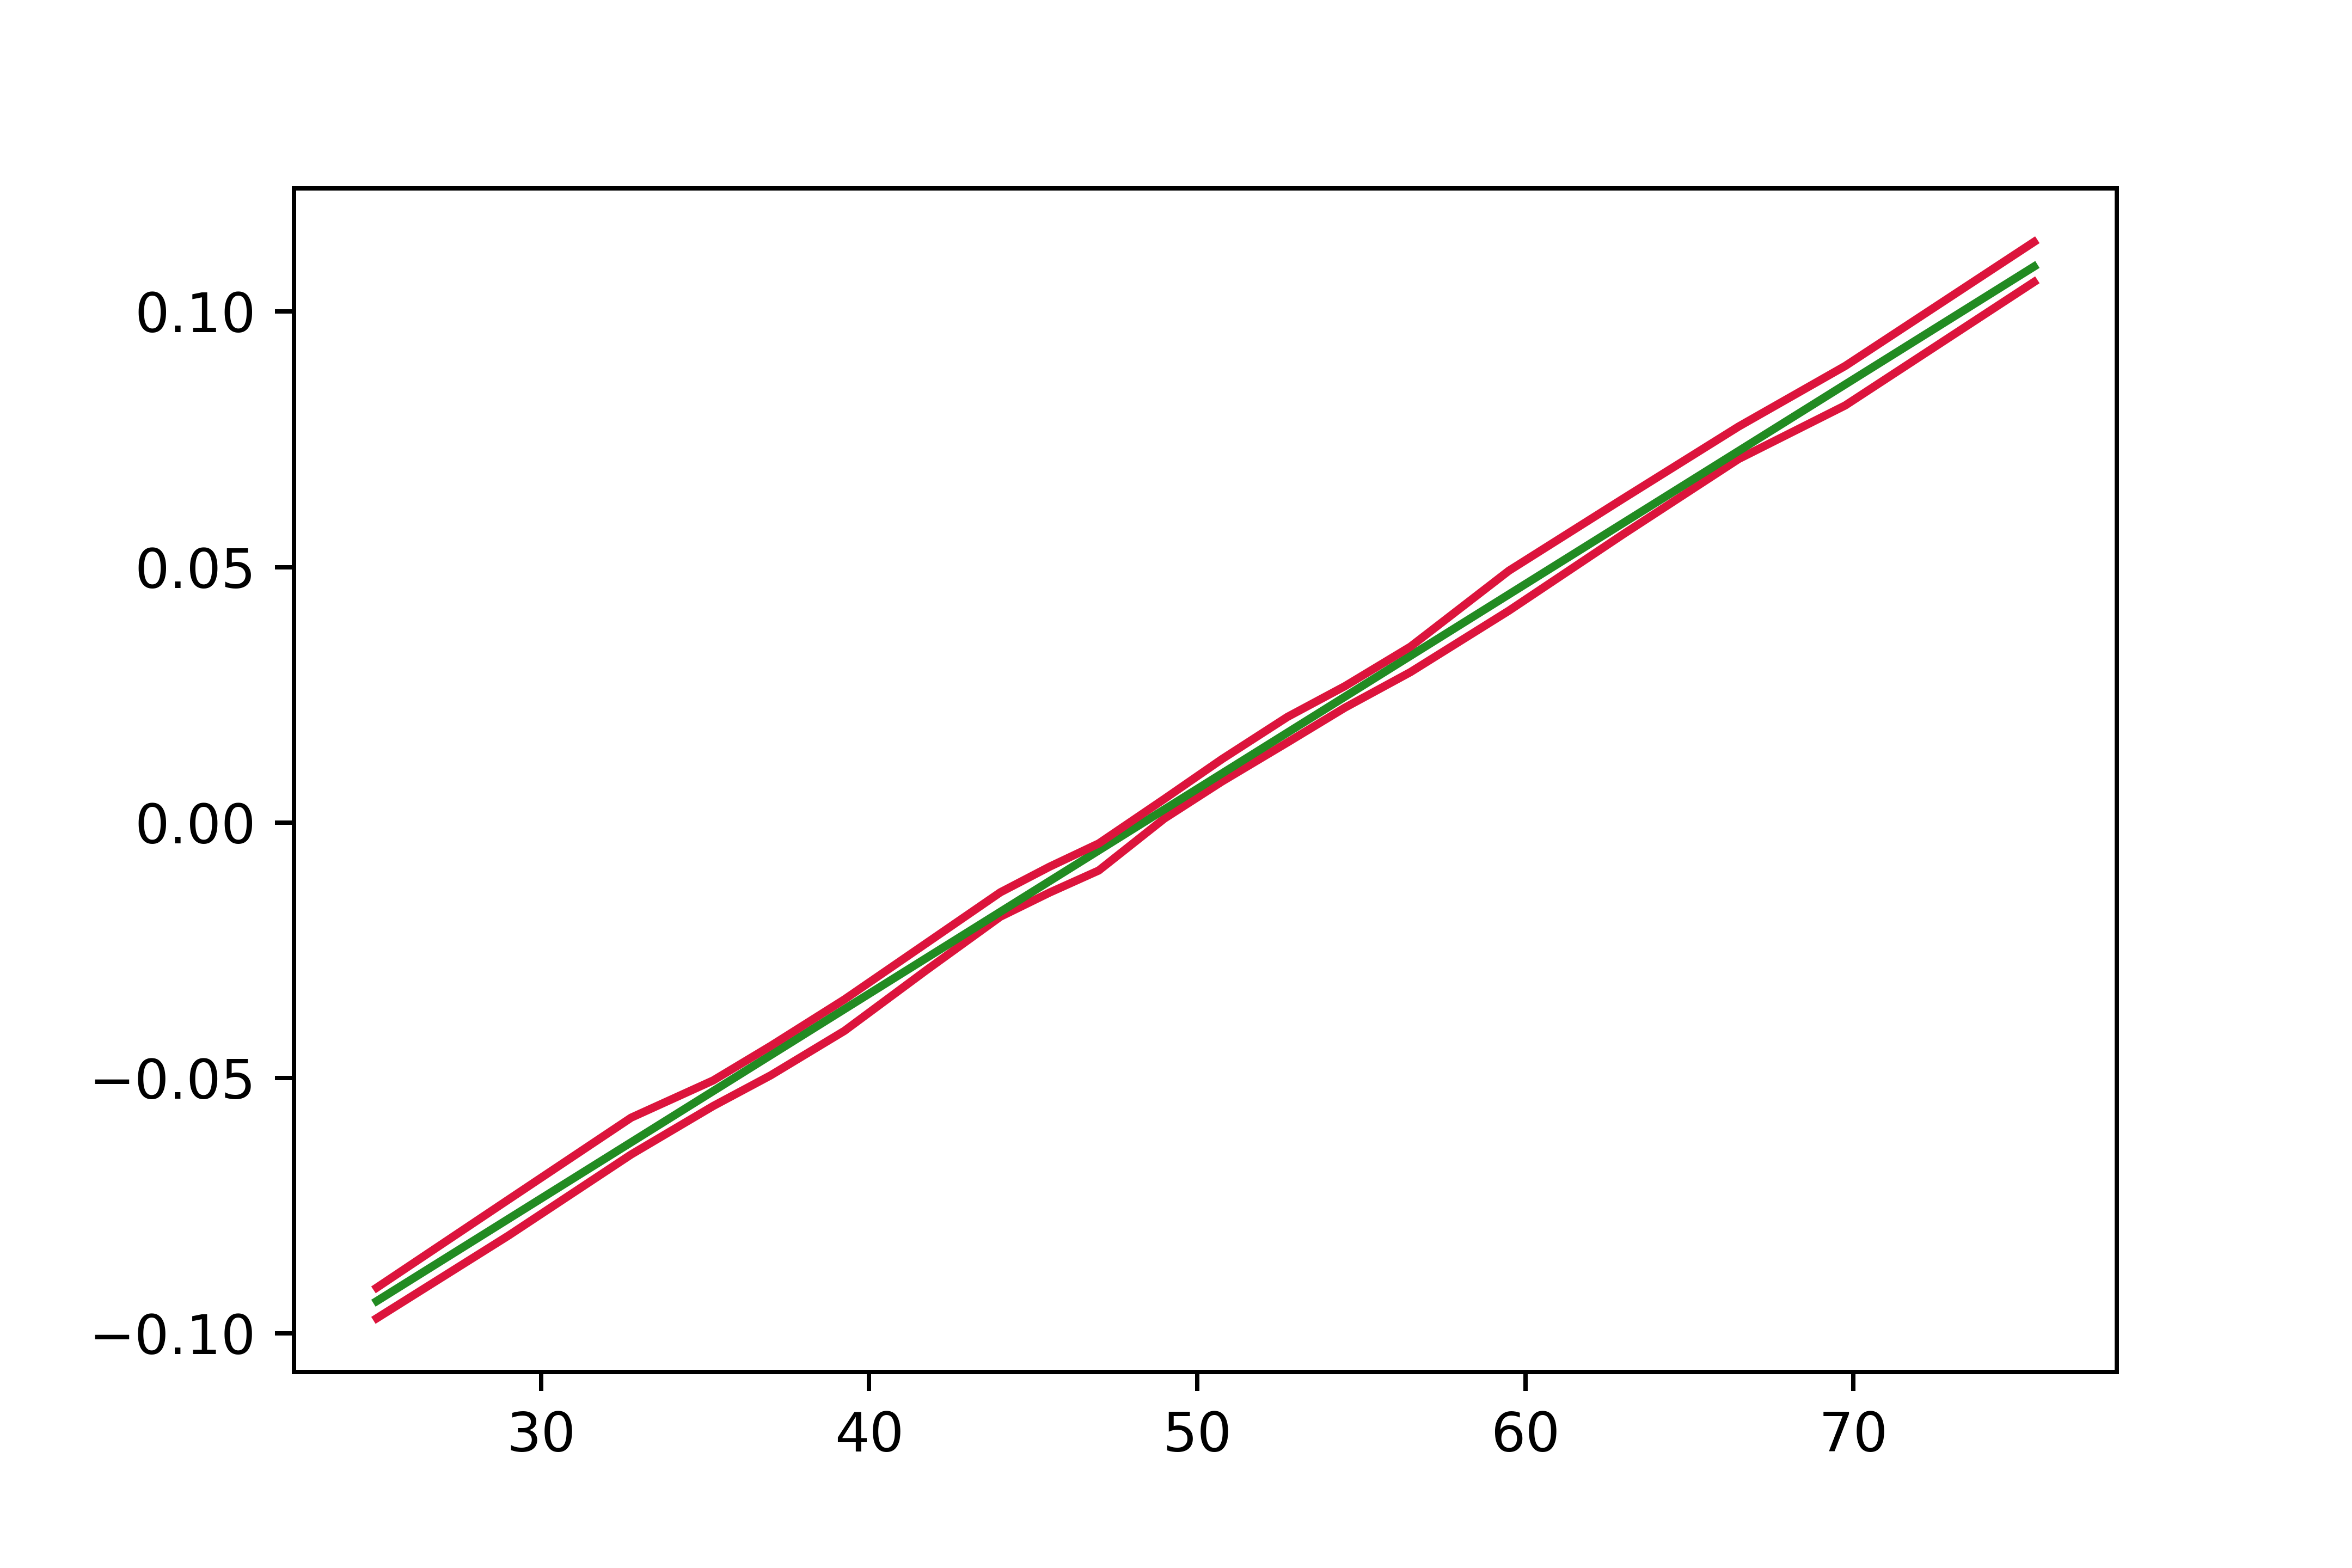
\includegraphics[width=\linewidth]{figures/ALE/chFDexp/spec3_linear_AGE.png}
        \caption{Spec 3 - linear}
    \end{subfigure}%
    \begin{subfigure}{0.5\linewidth}
        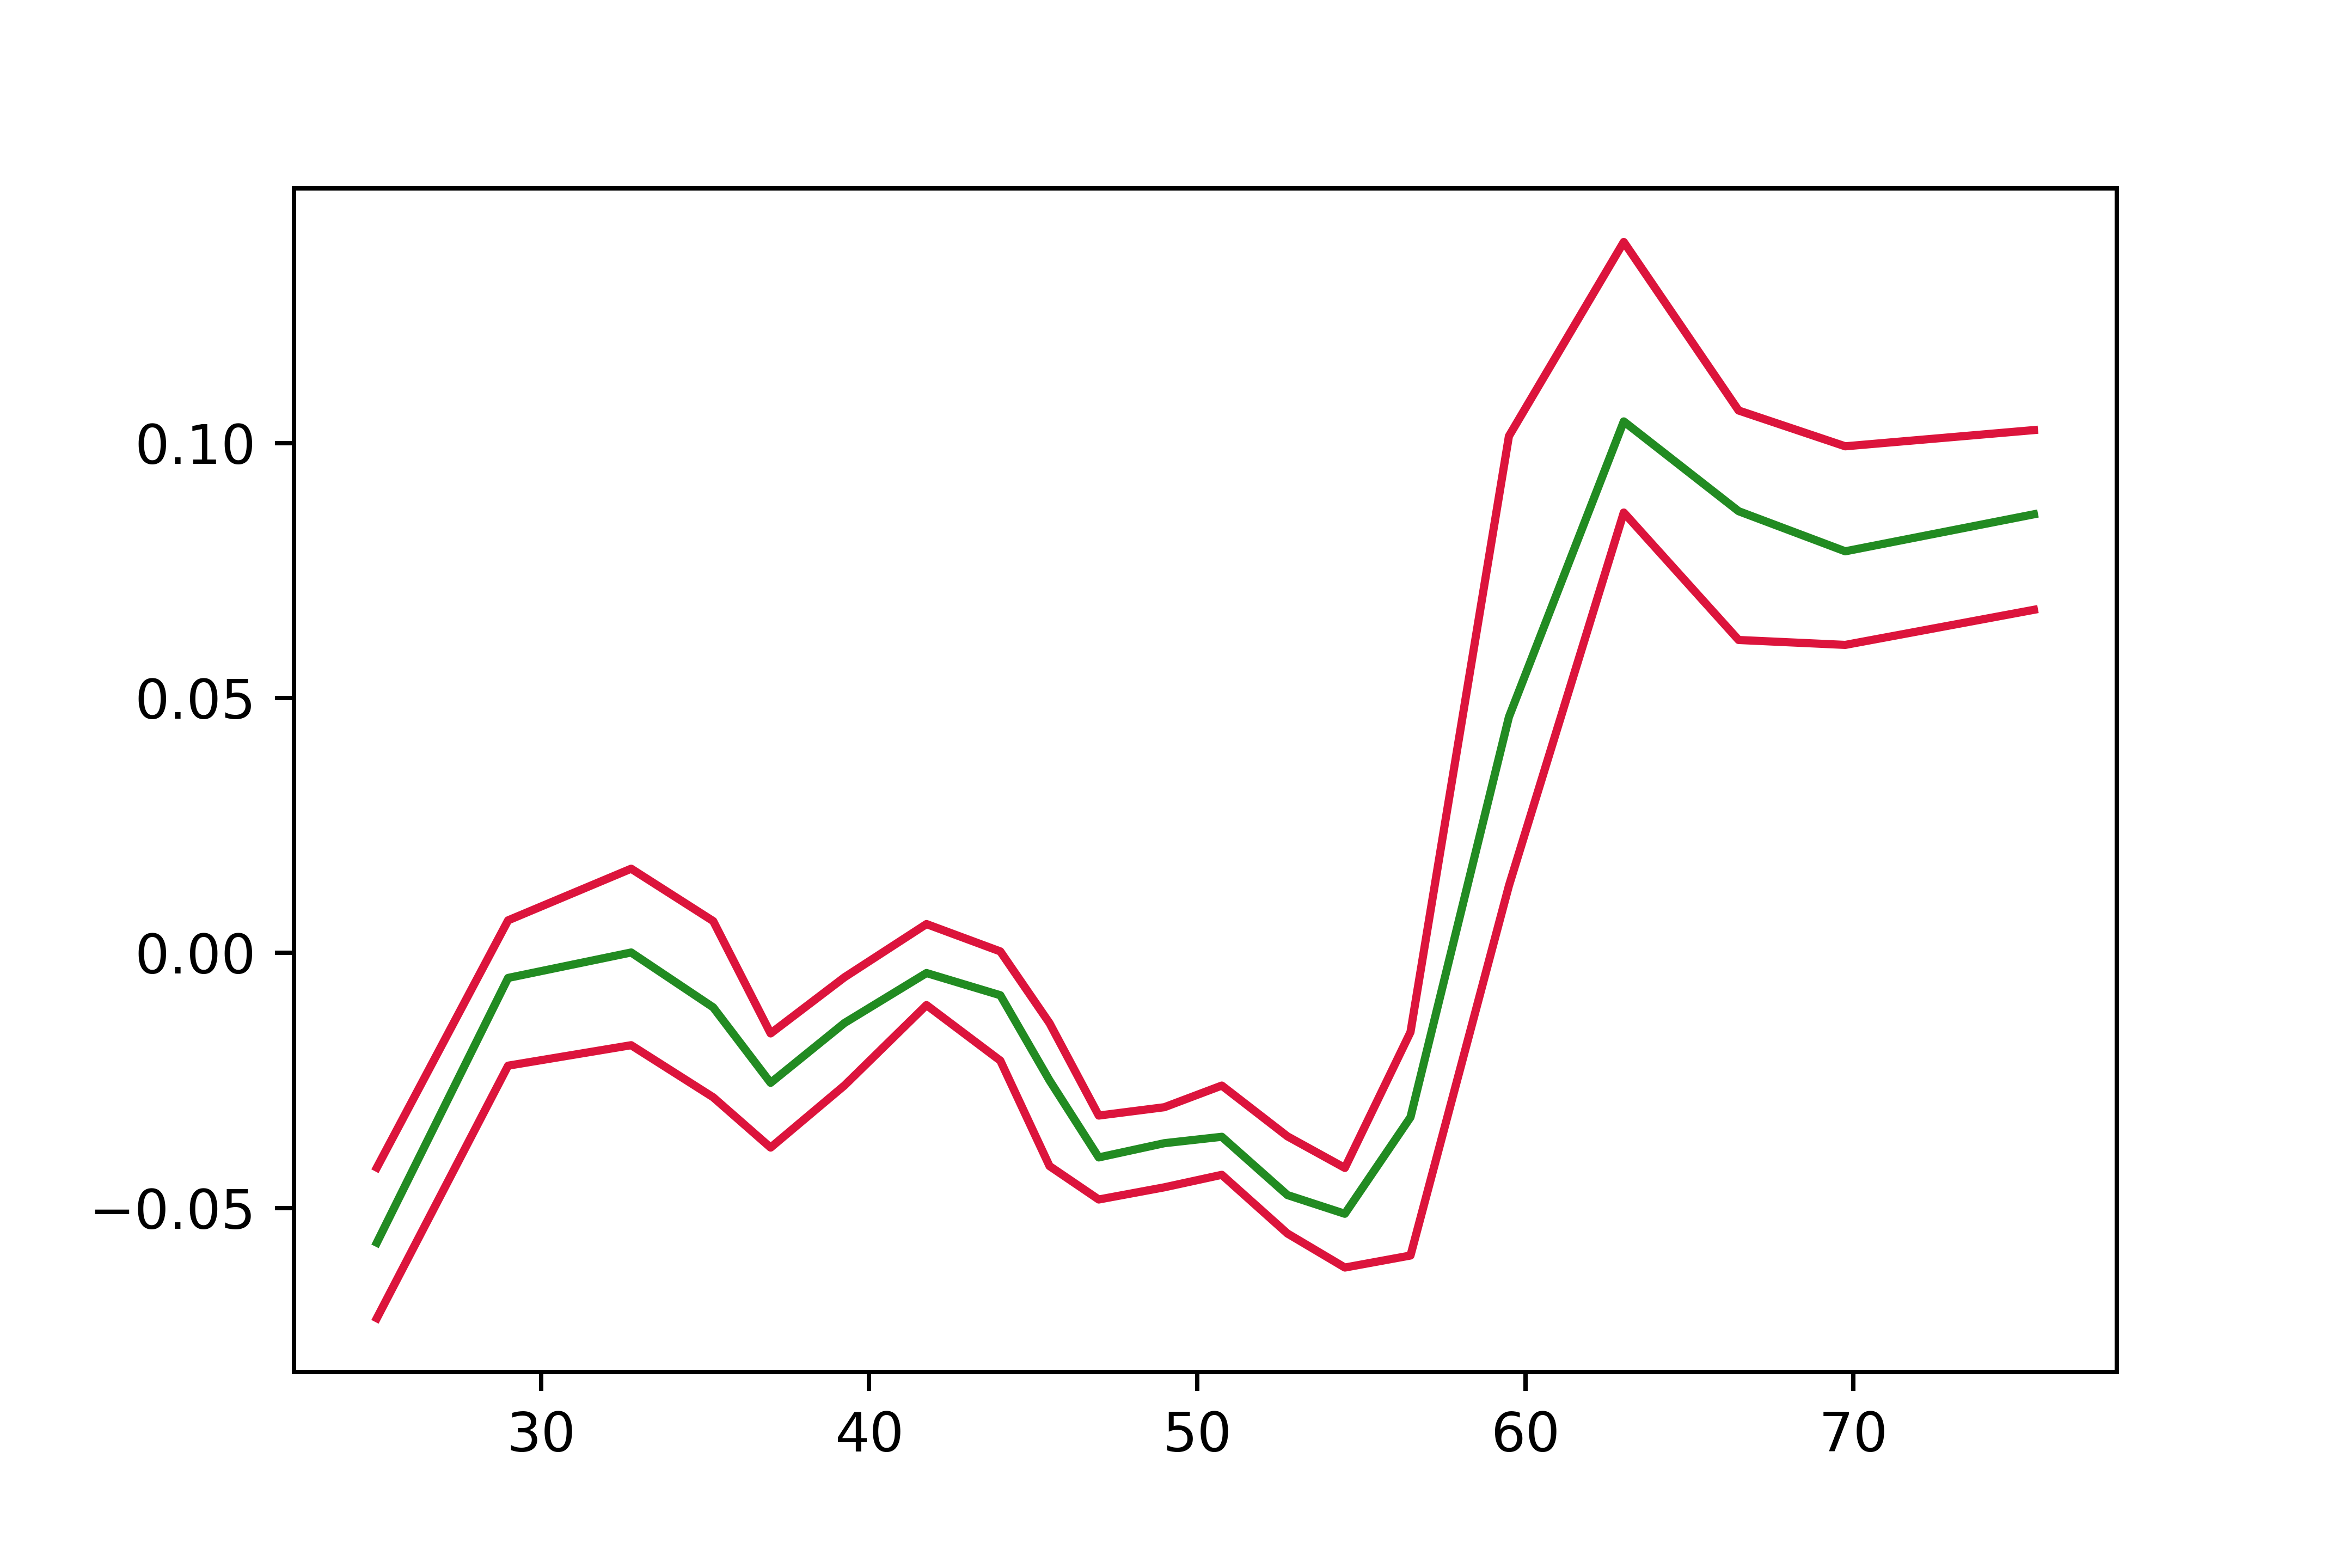
\includegraphics[width=\linewidth]{figures/ALE/chFDexp/spec3_cf_AGE.png}
        \caption{Spec 3 - causal forest}
    \end{subfigure}
    \caption{ALE of AGE - strictly non-durables}
    \label{app:ale_age_fd}
\end{figure}

%! SND - Fin Stat
\begin{figure}[h]
    \centering
    \begin{subfigure}{0.5\linewidth}
        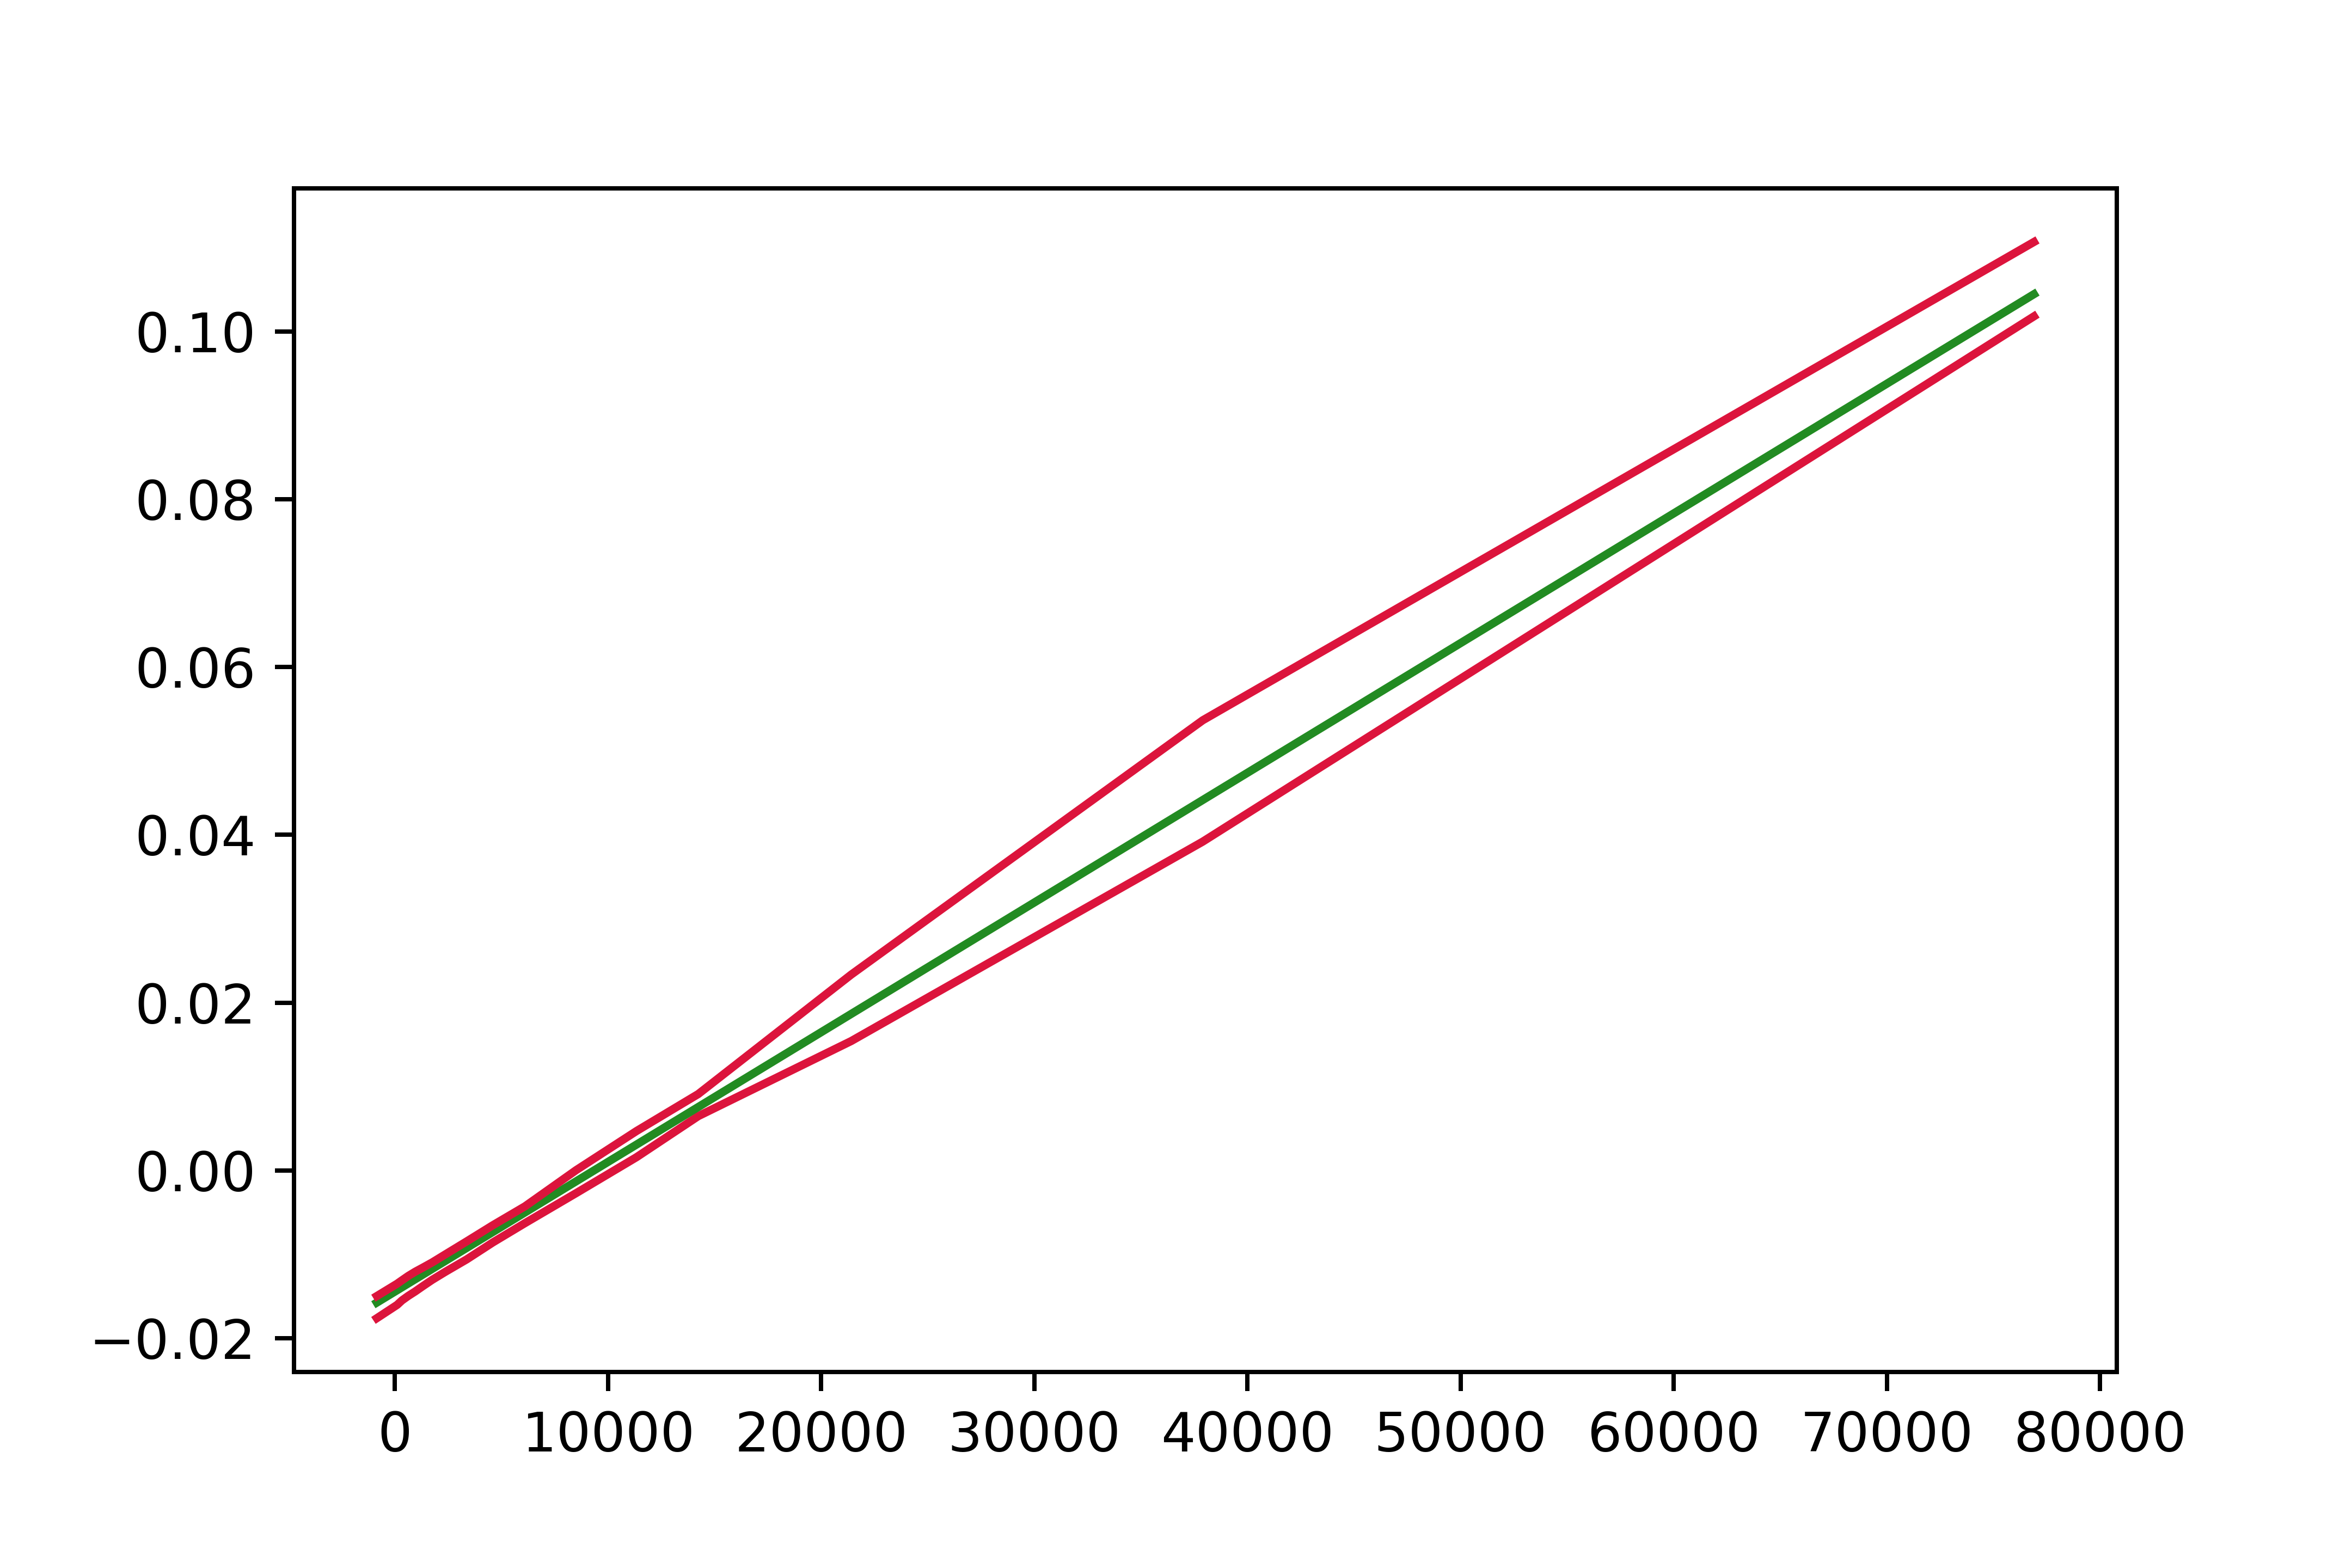
\includegraphics[width=\linewidth]{figures/ALE/chFDexp/spec3_linear_liqassii.png}
        \caption{Liquid Assets - linear}
    \end{subfigure}%
    \begin{subfigure}{0.5\linewidth}
        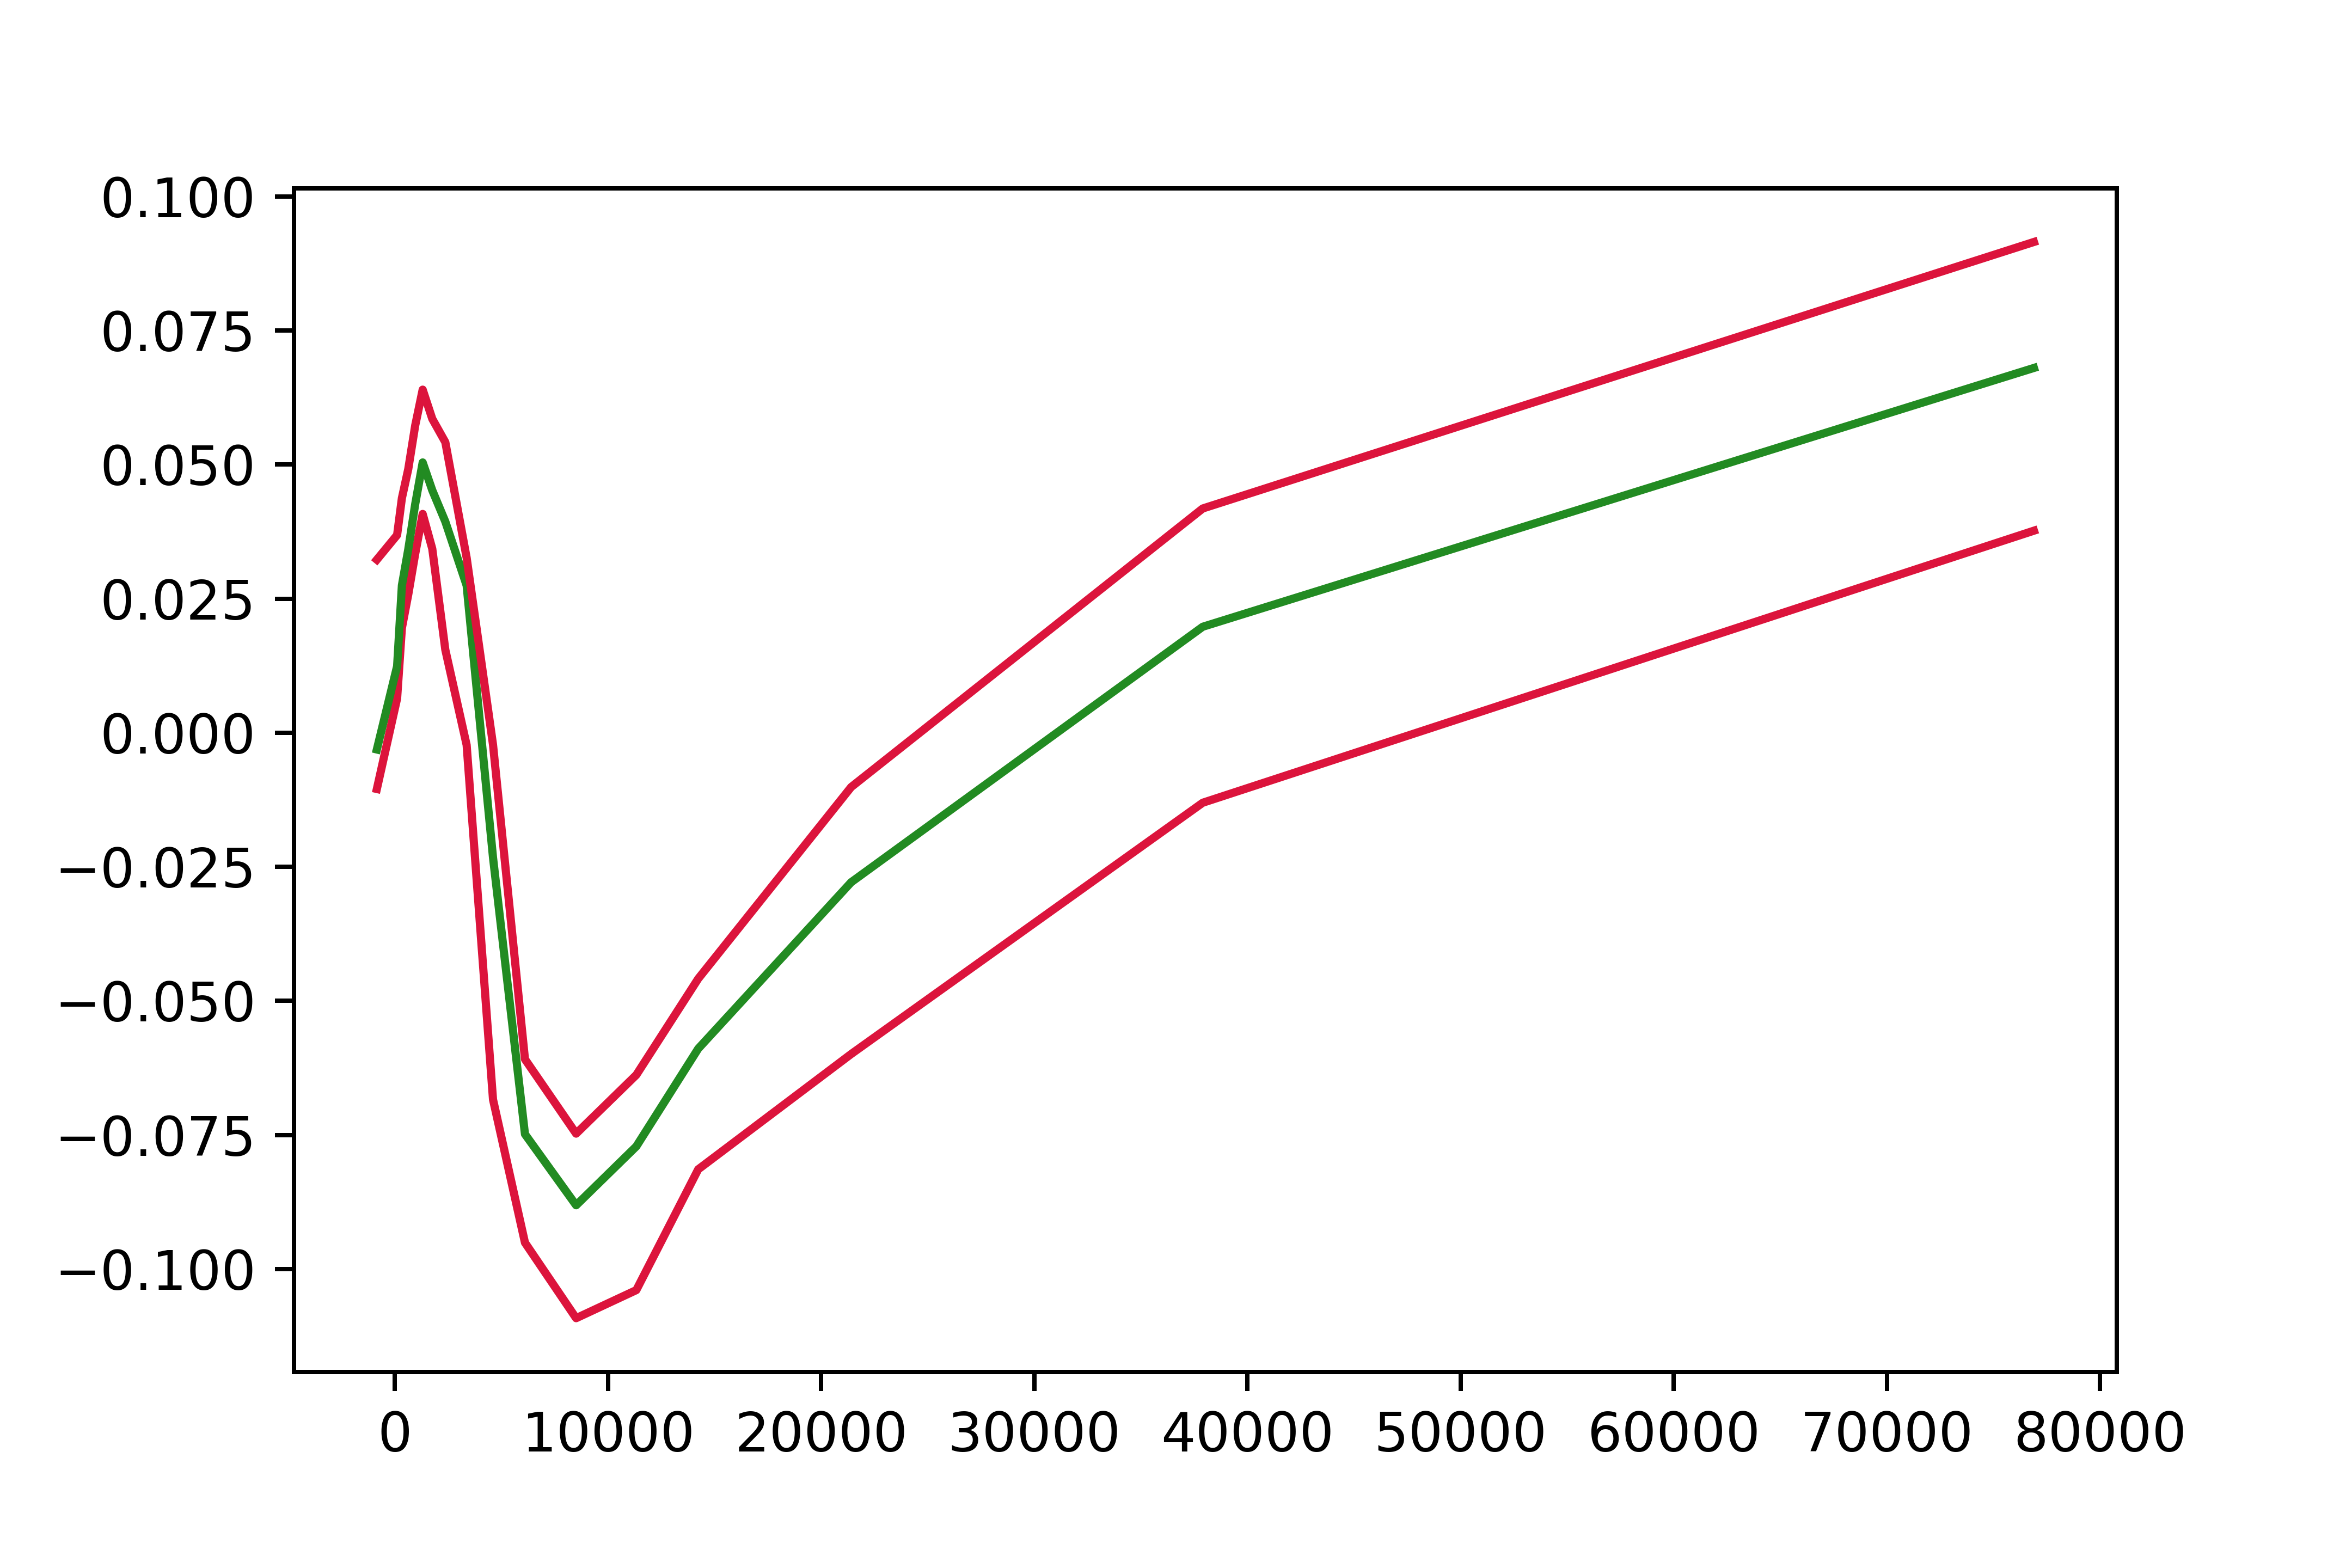
\includegraphics[width=\linewidth]{figures/ALE/chFDexp/spec3_cf_liqassii.png}
        \caption{Liquid Assets - causal forest}
    \end{subfigure}

    \begin{subfigure}{0.5\linewidth}
        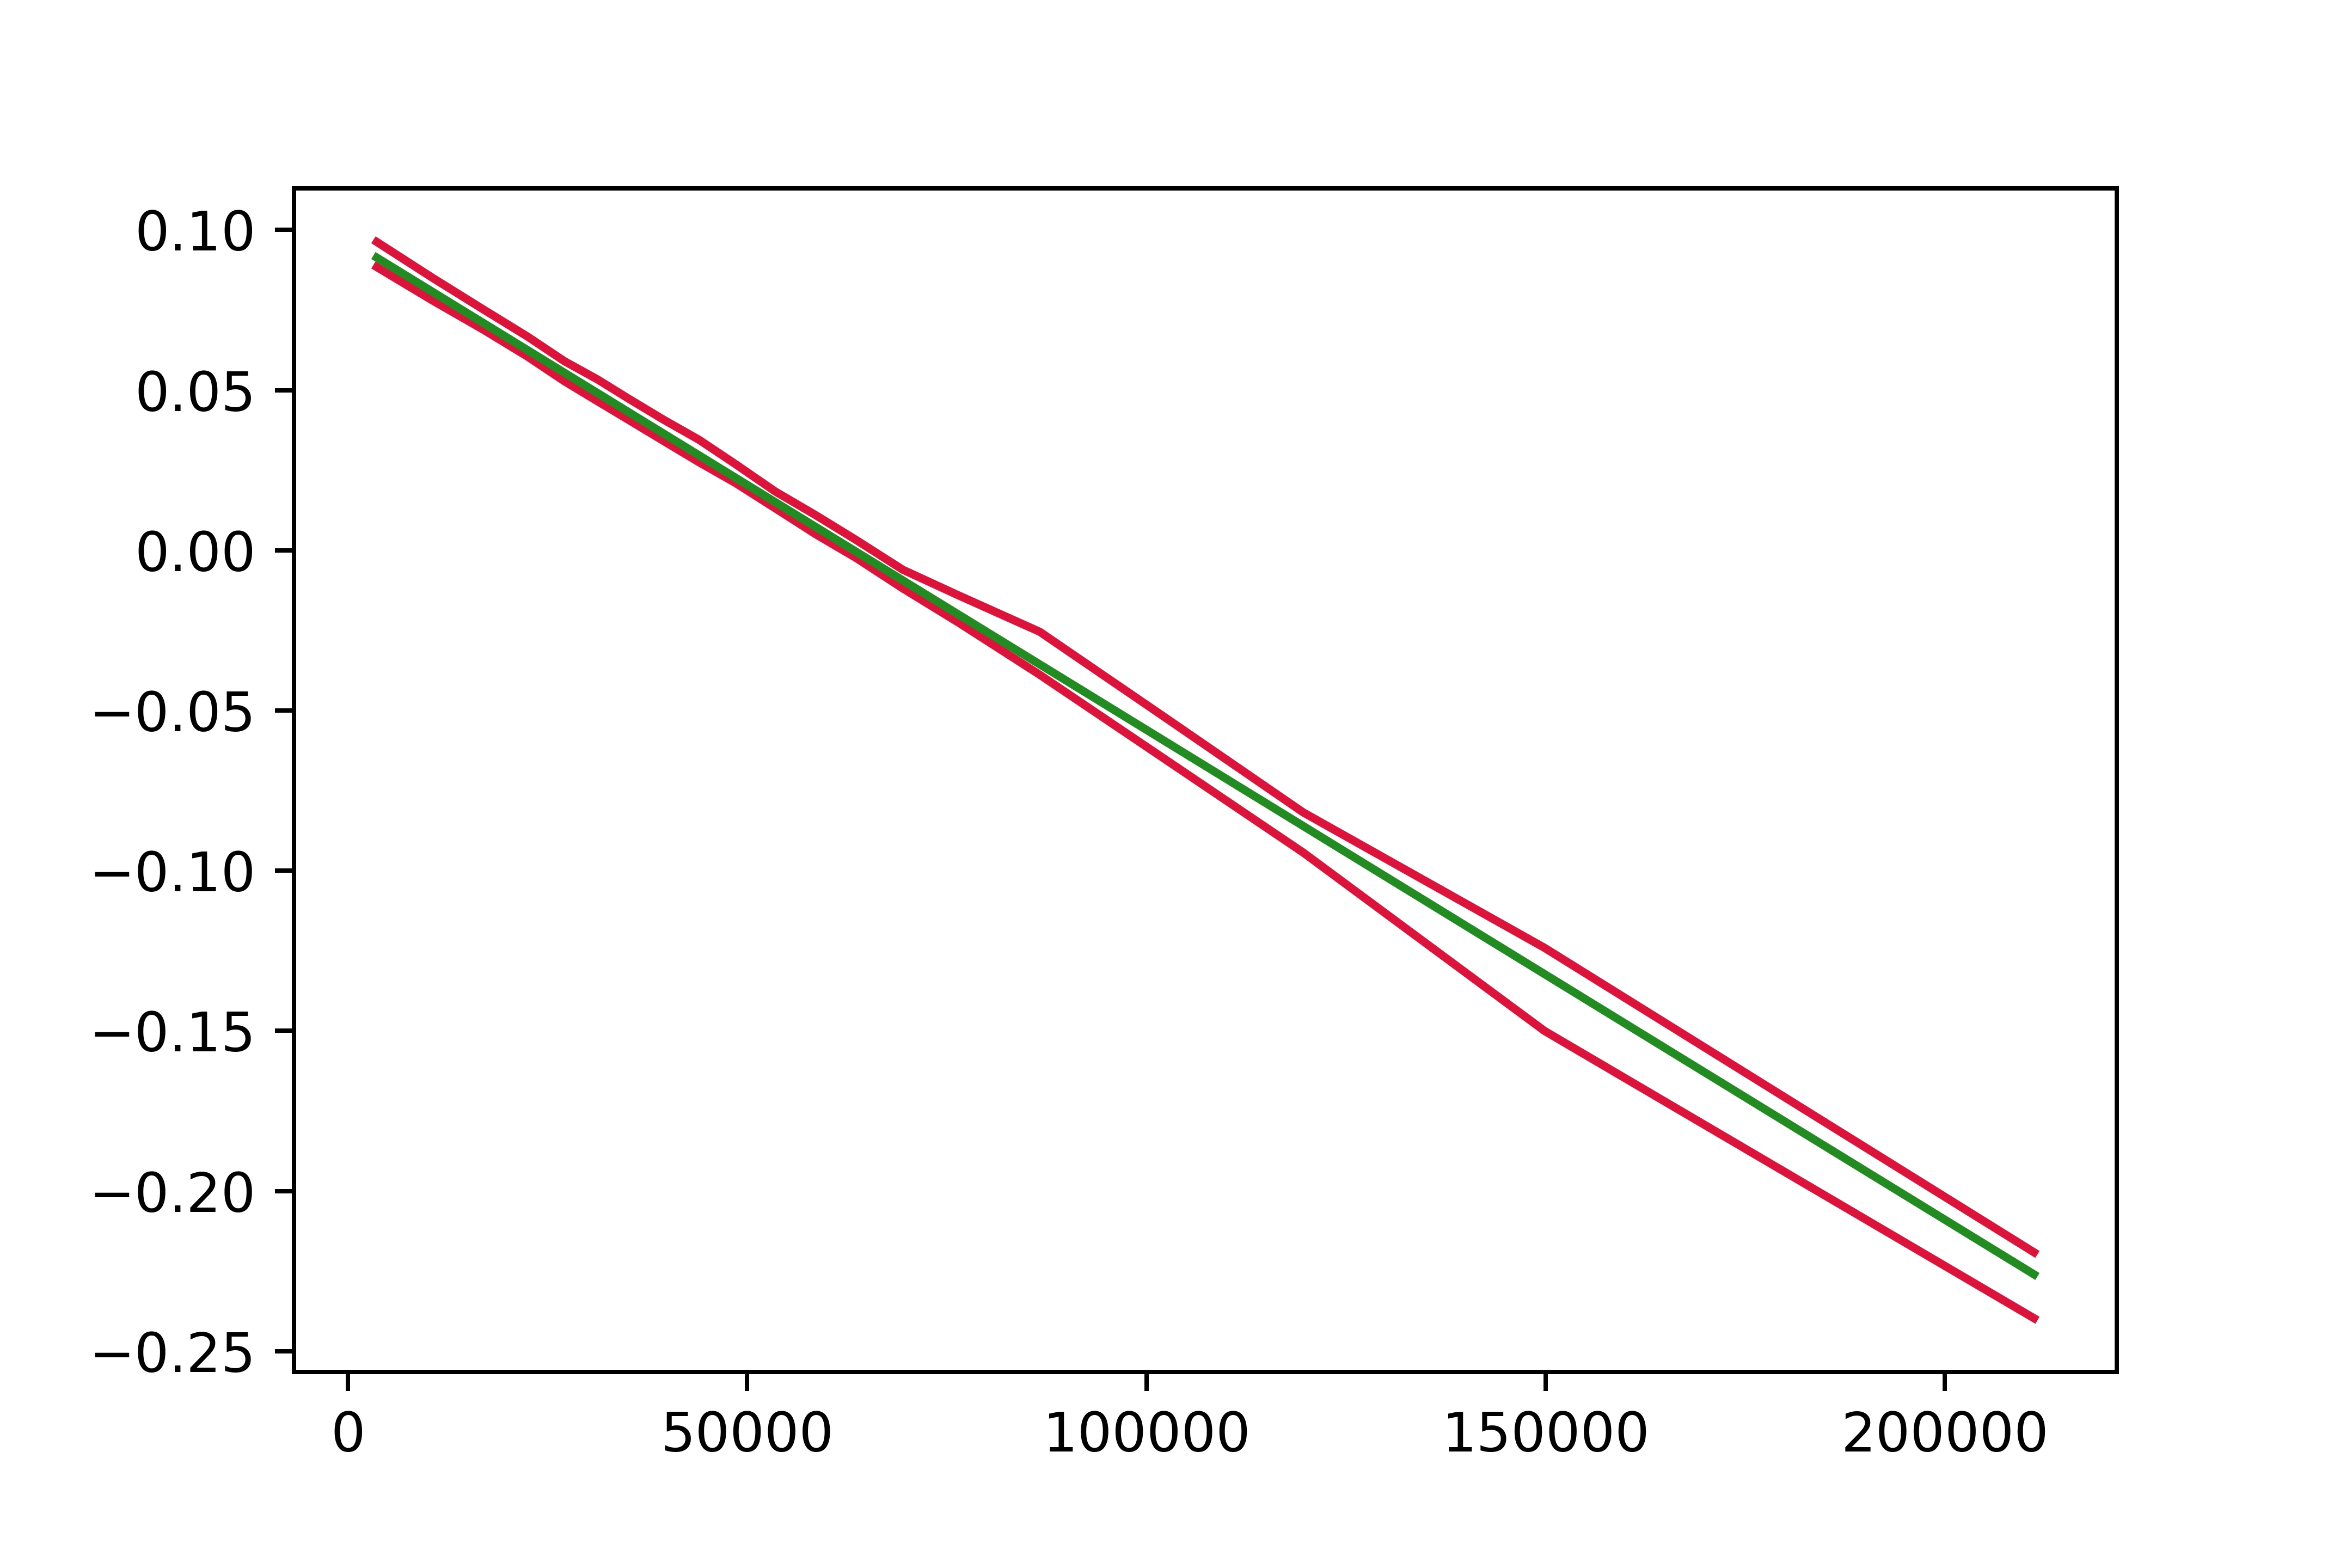
\includegraphics[width=\linewidth]{figures/ALE/chFDexp/spec3_linear_FSALARYM.png}
        \caption{Salary - linear}
    \end{subfigure}%
    \begin{subfigure}{0.5\linewidth}
        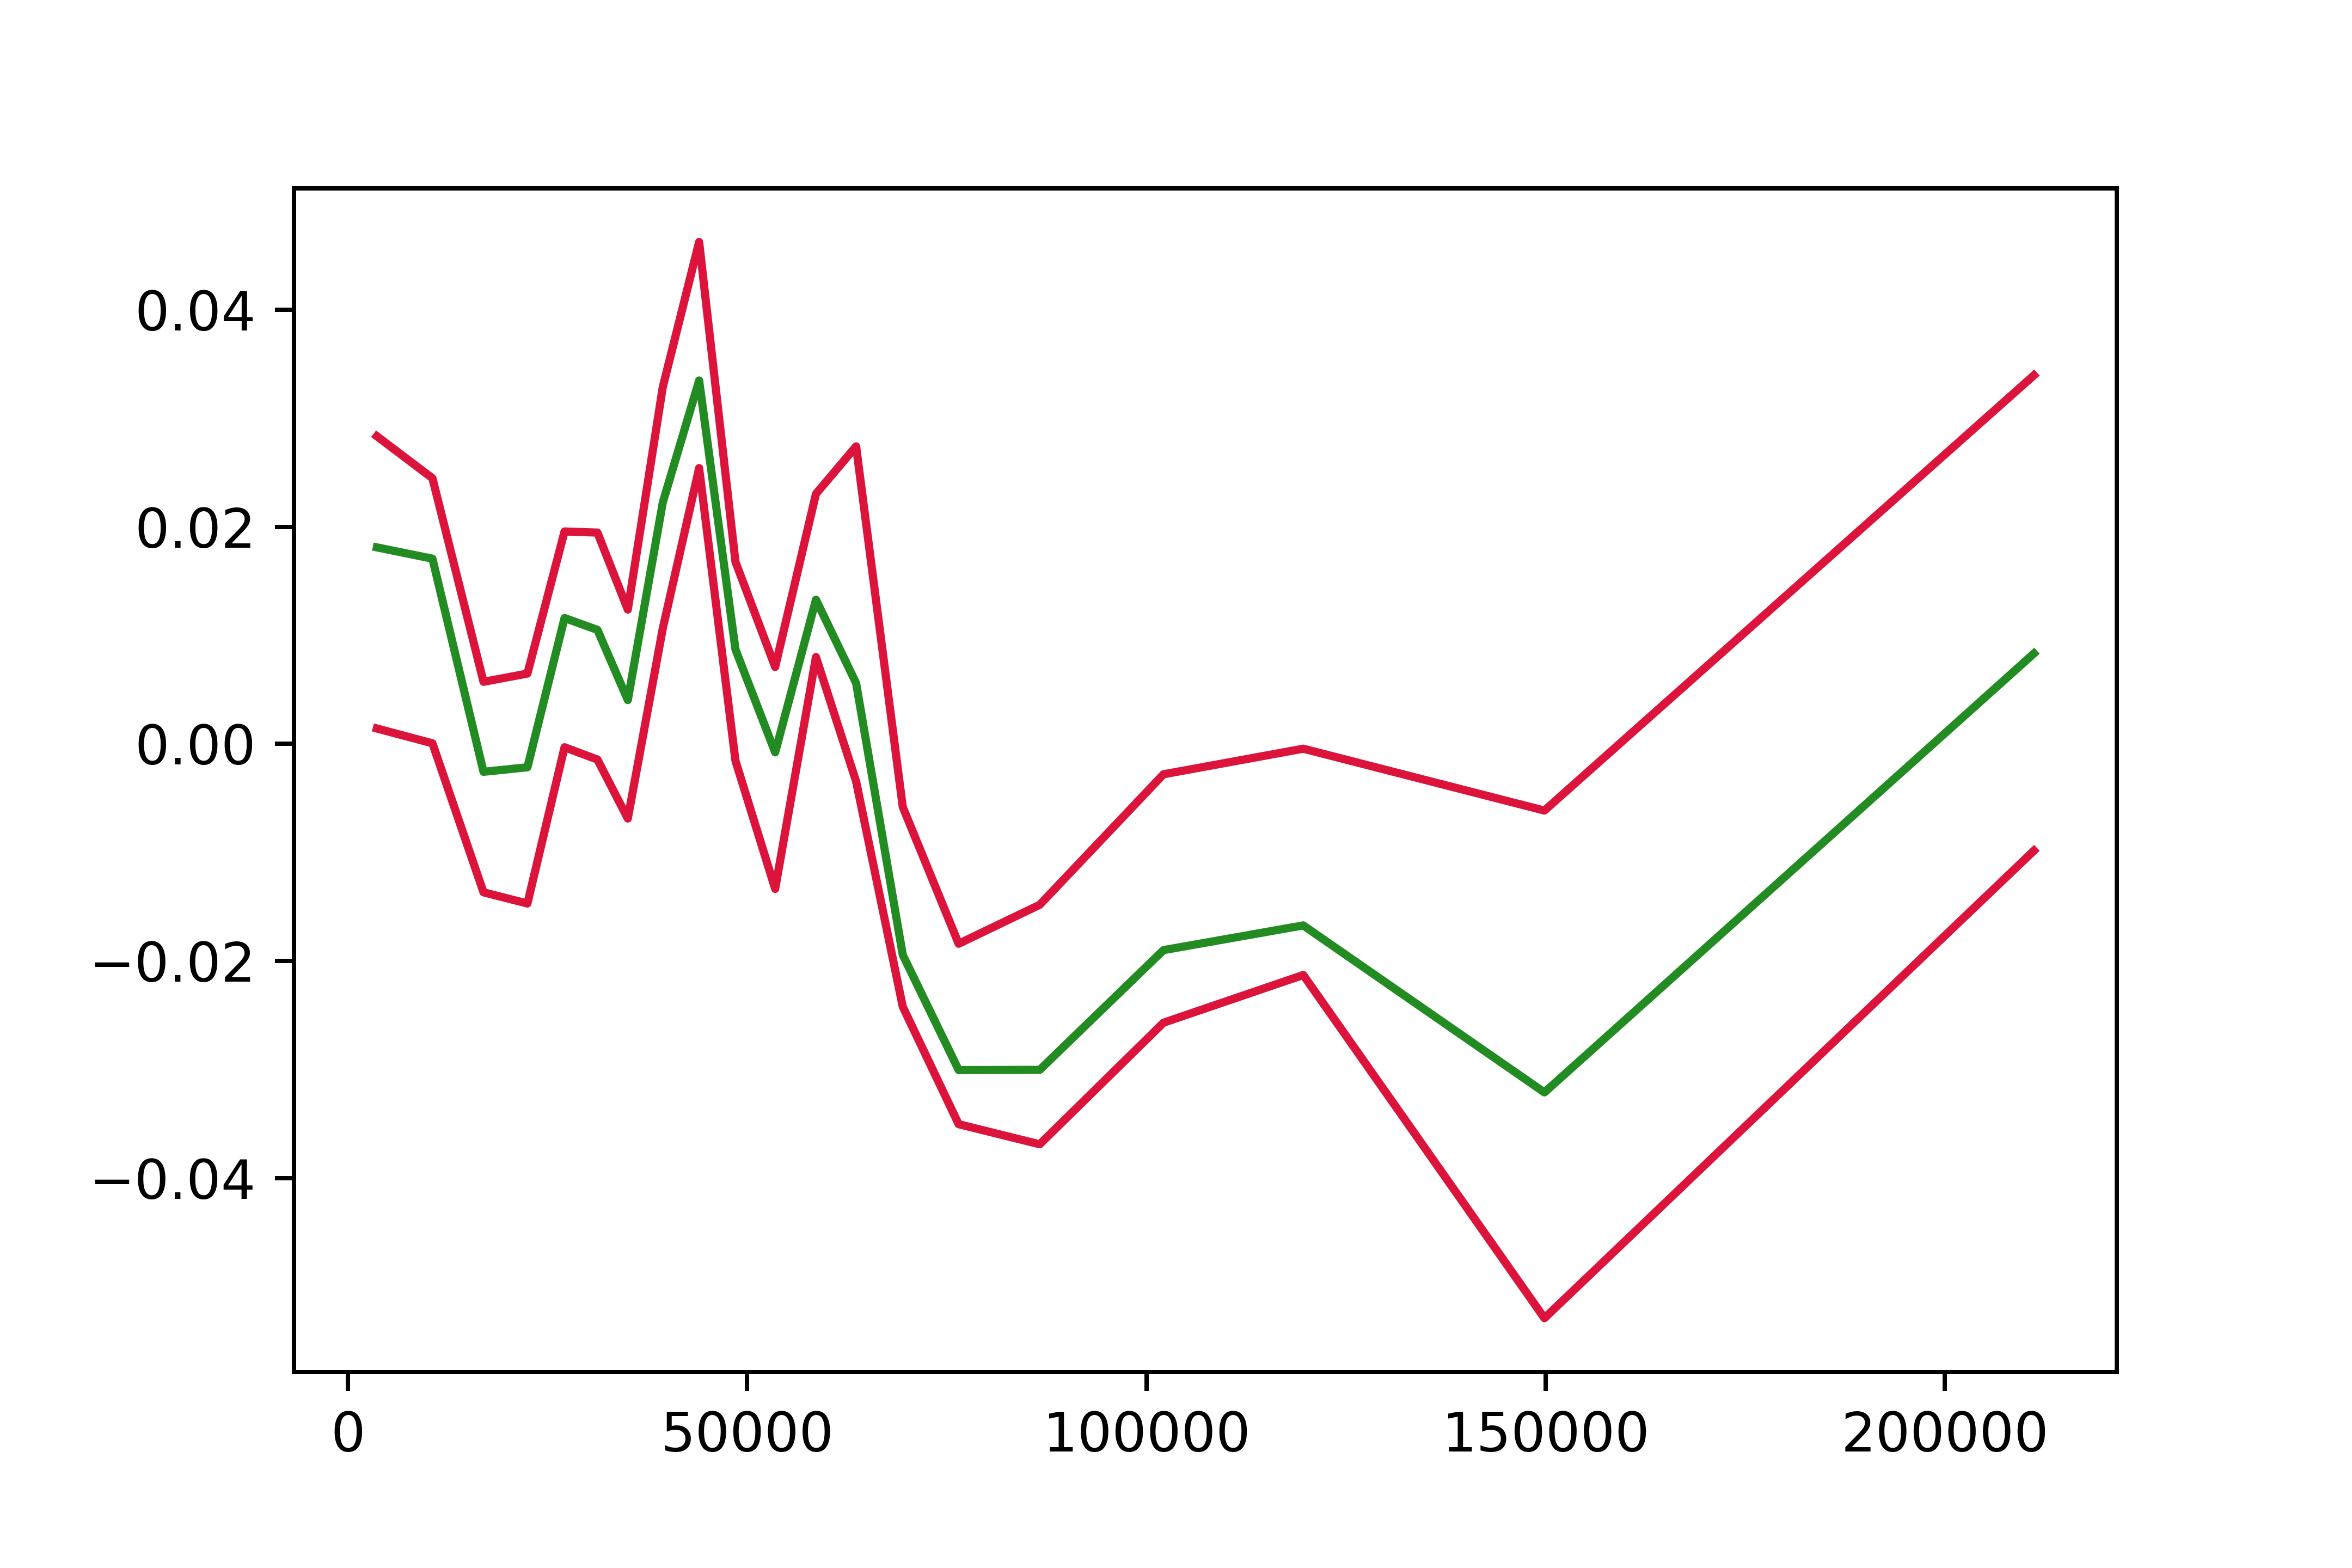
\includegraphics[width=\linewidth]{figures/ALE/chFDexp/spec3_cf_FSALARYM.png}
        \caption{Salary - causal forest}
    \end{subfigure}

    \begin{subfigure}{0.5\linewidth}
        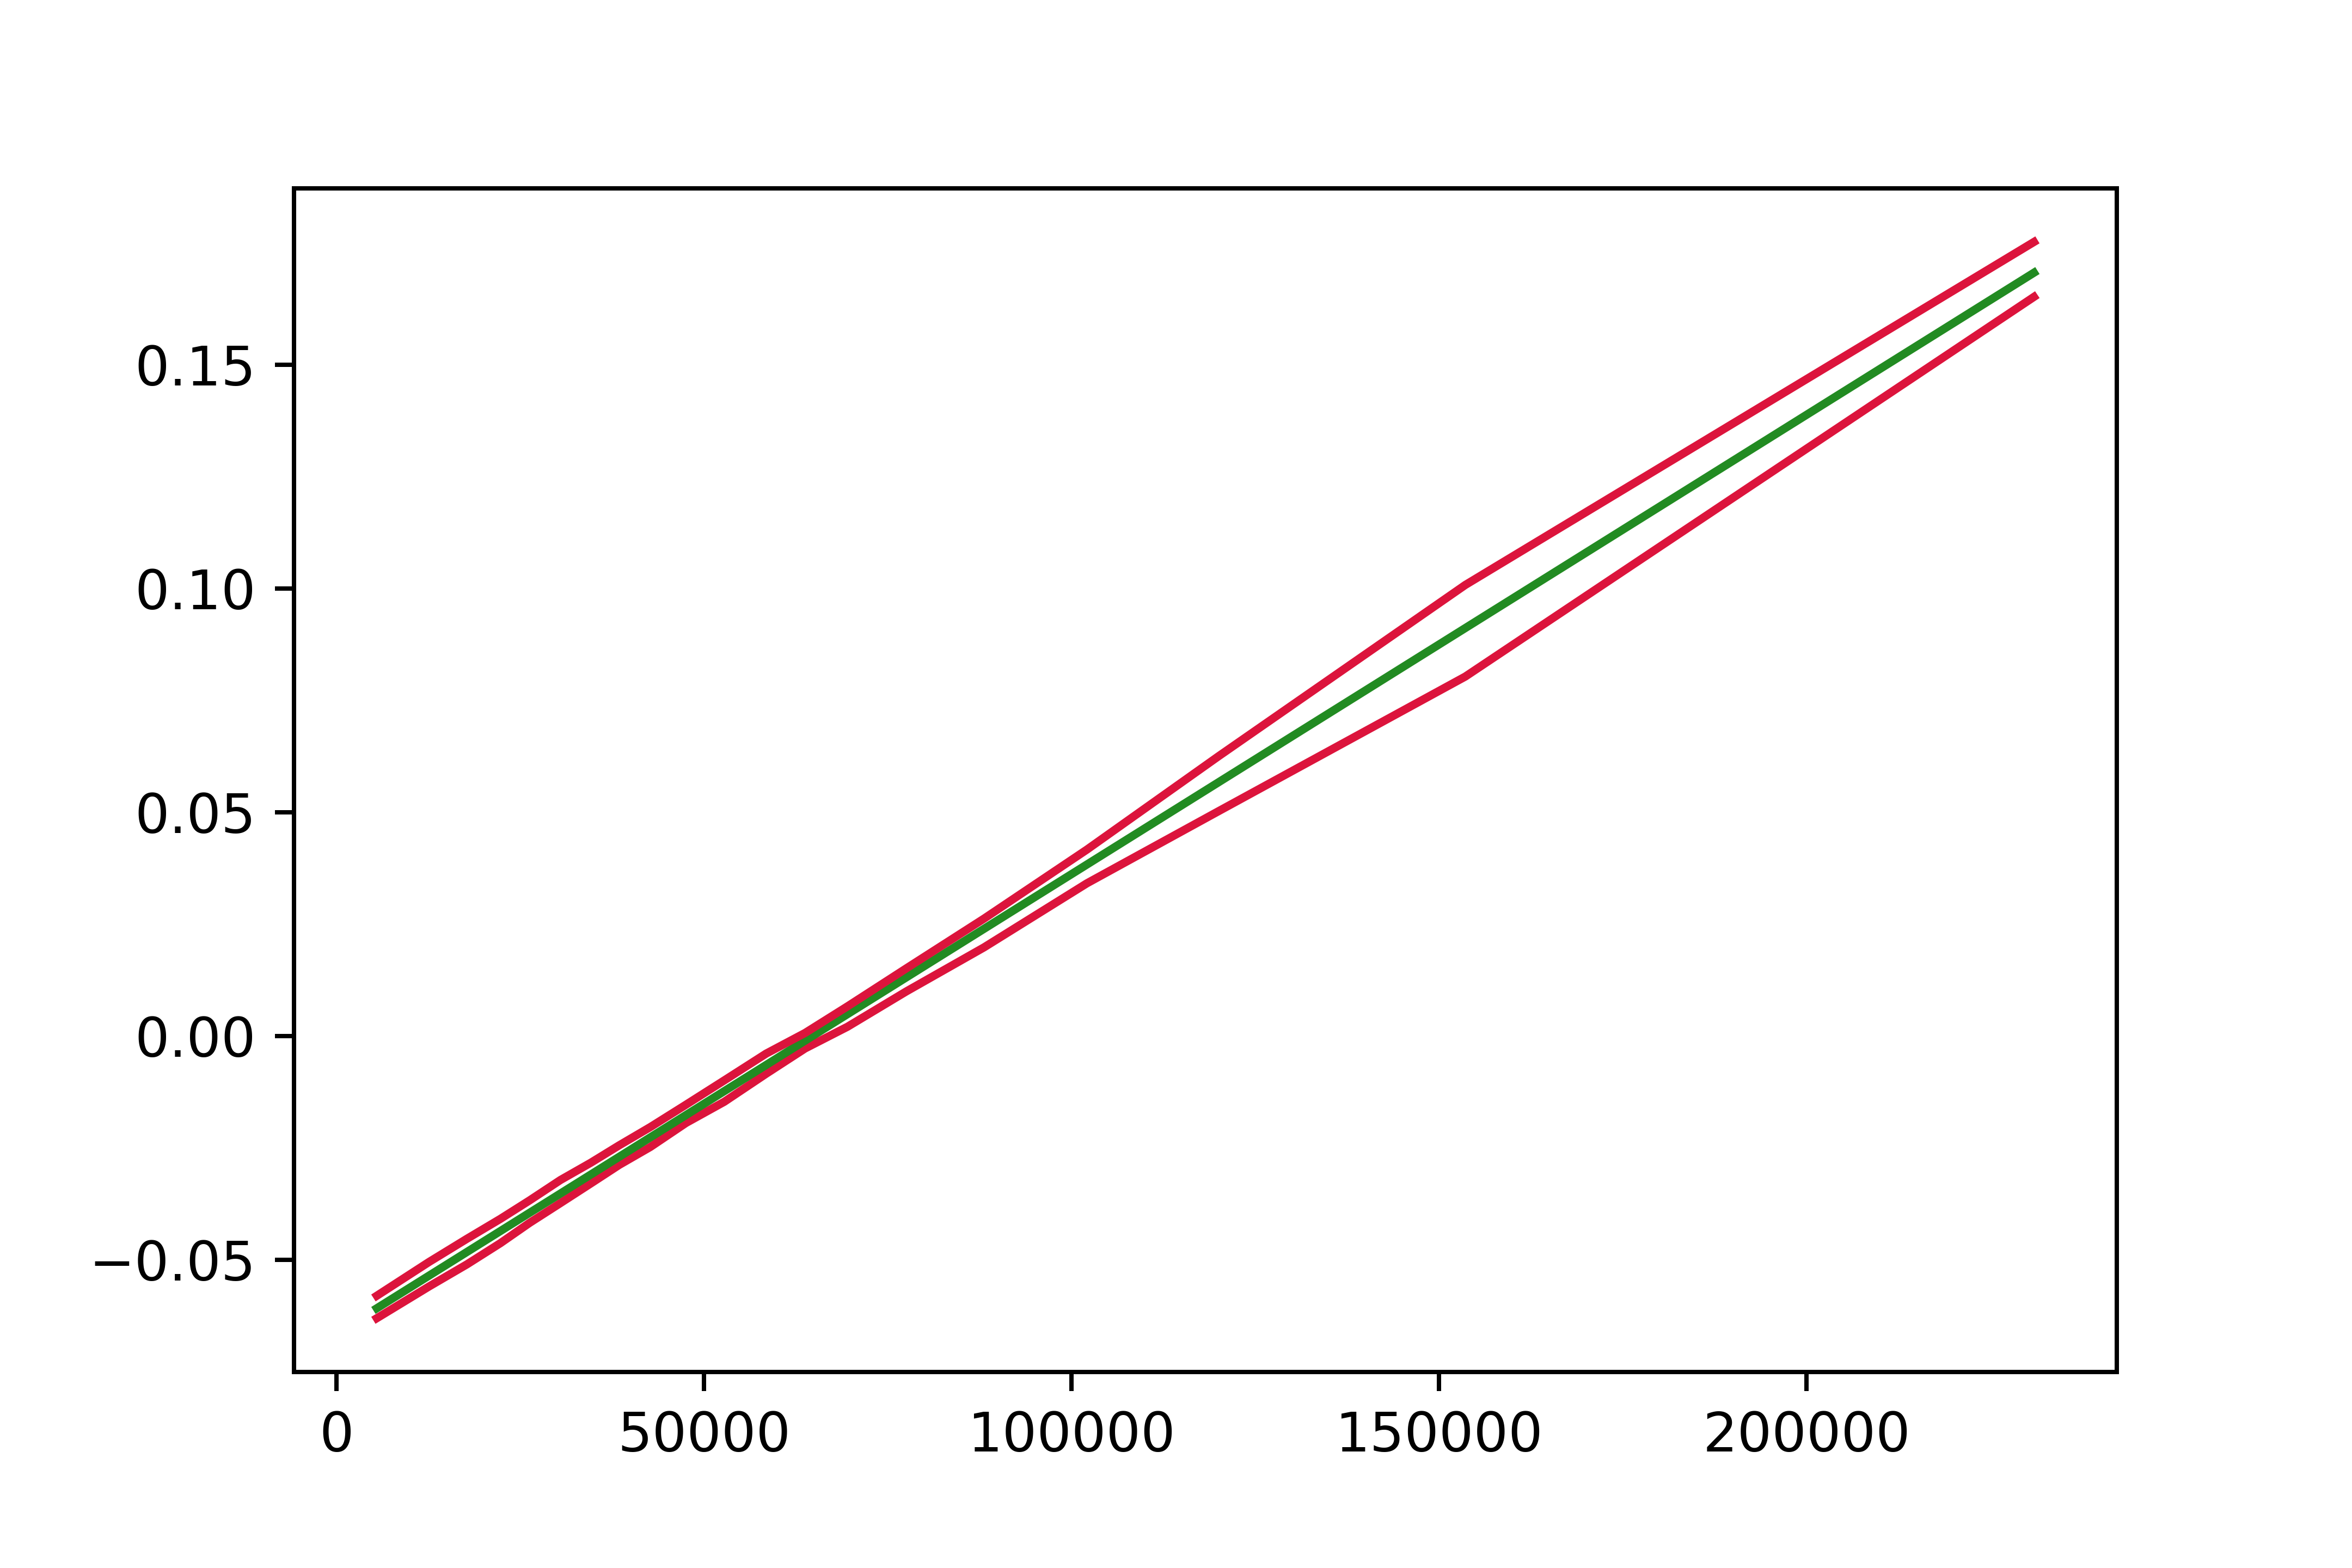
\includegraphics[width=\linewidth]{figures/ALE/chFDexp/spec3_linear_FINCBTXM.png}
        \caption{Income - linear}
    \end{subfigure}%
    \begin{subfigure}{0.5\linewidth}
        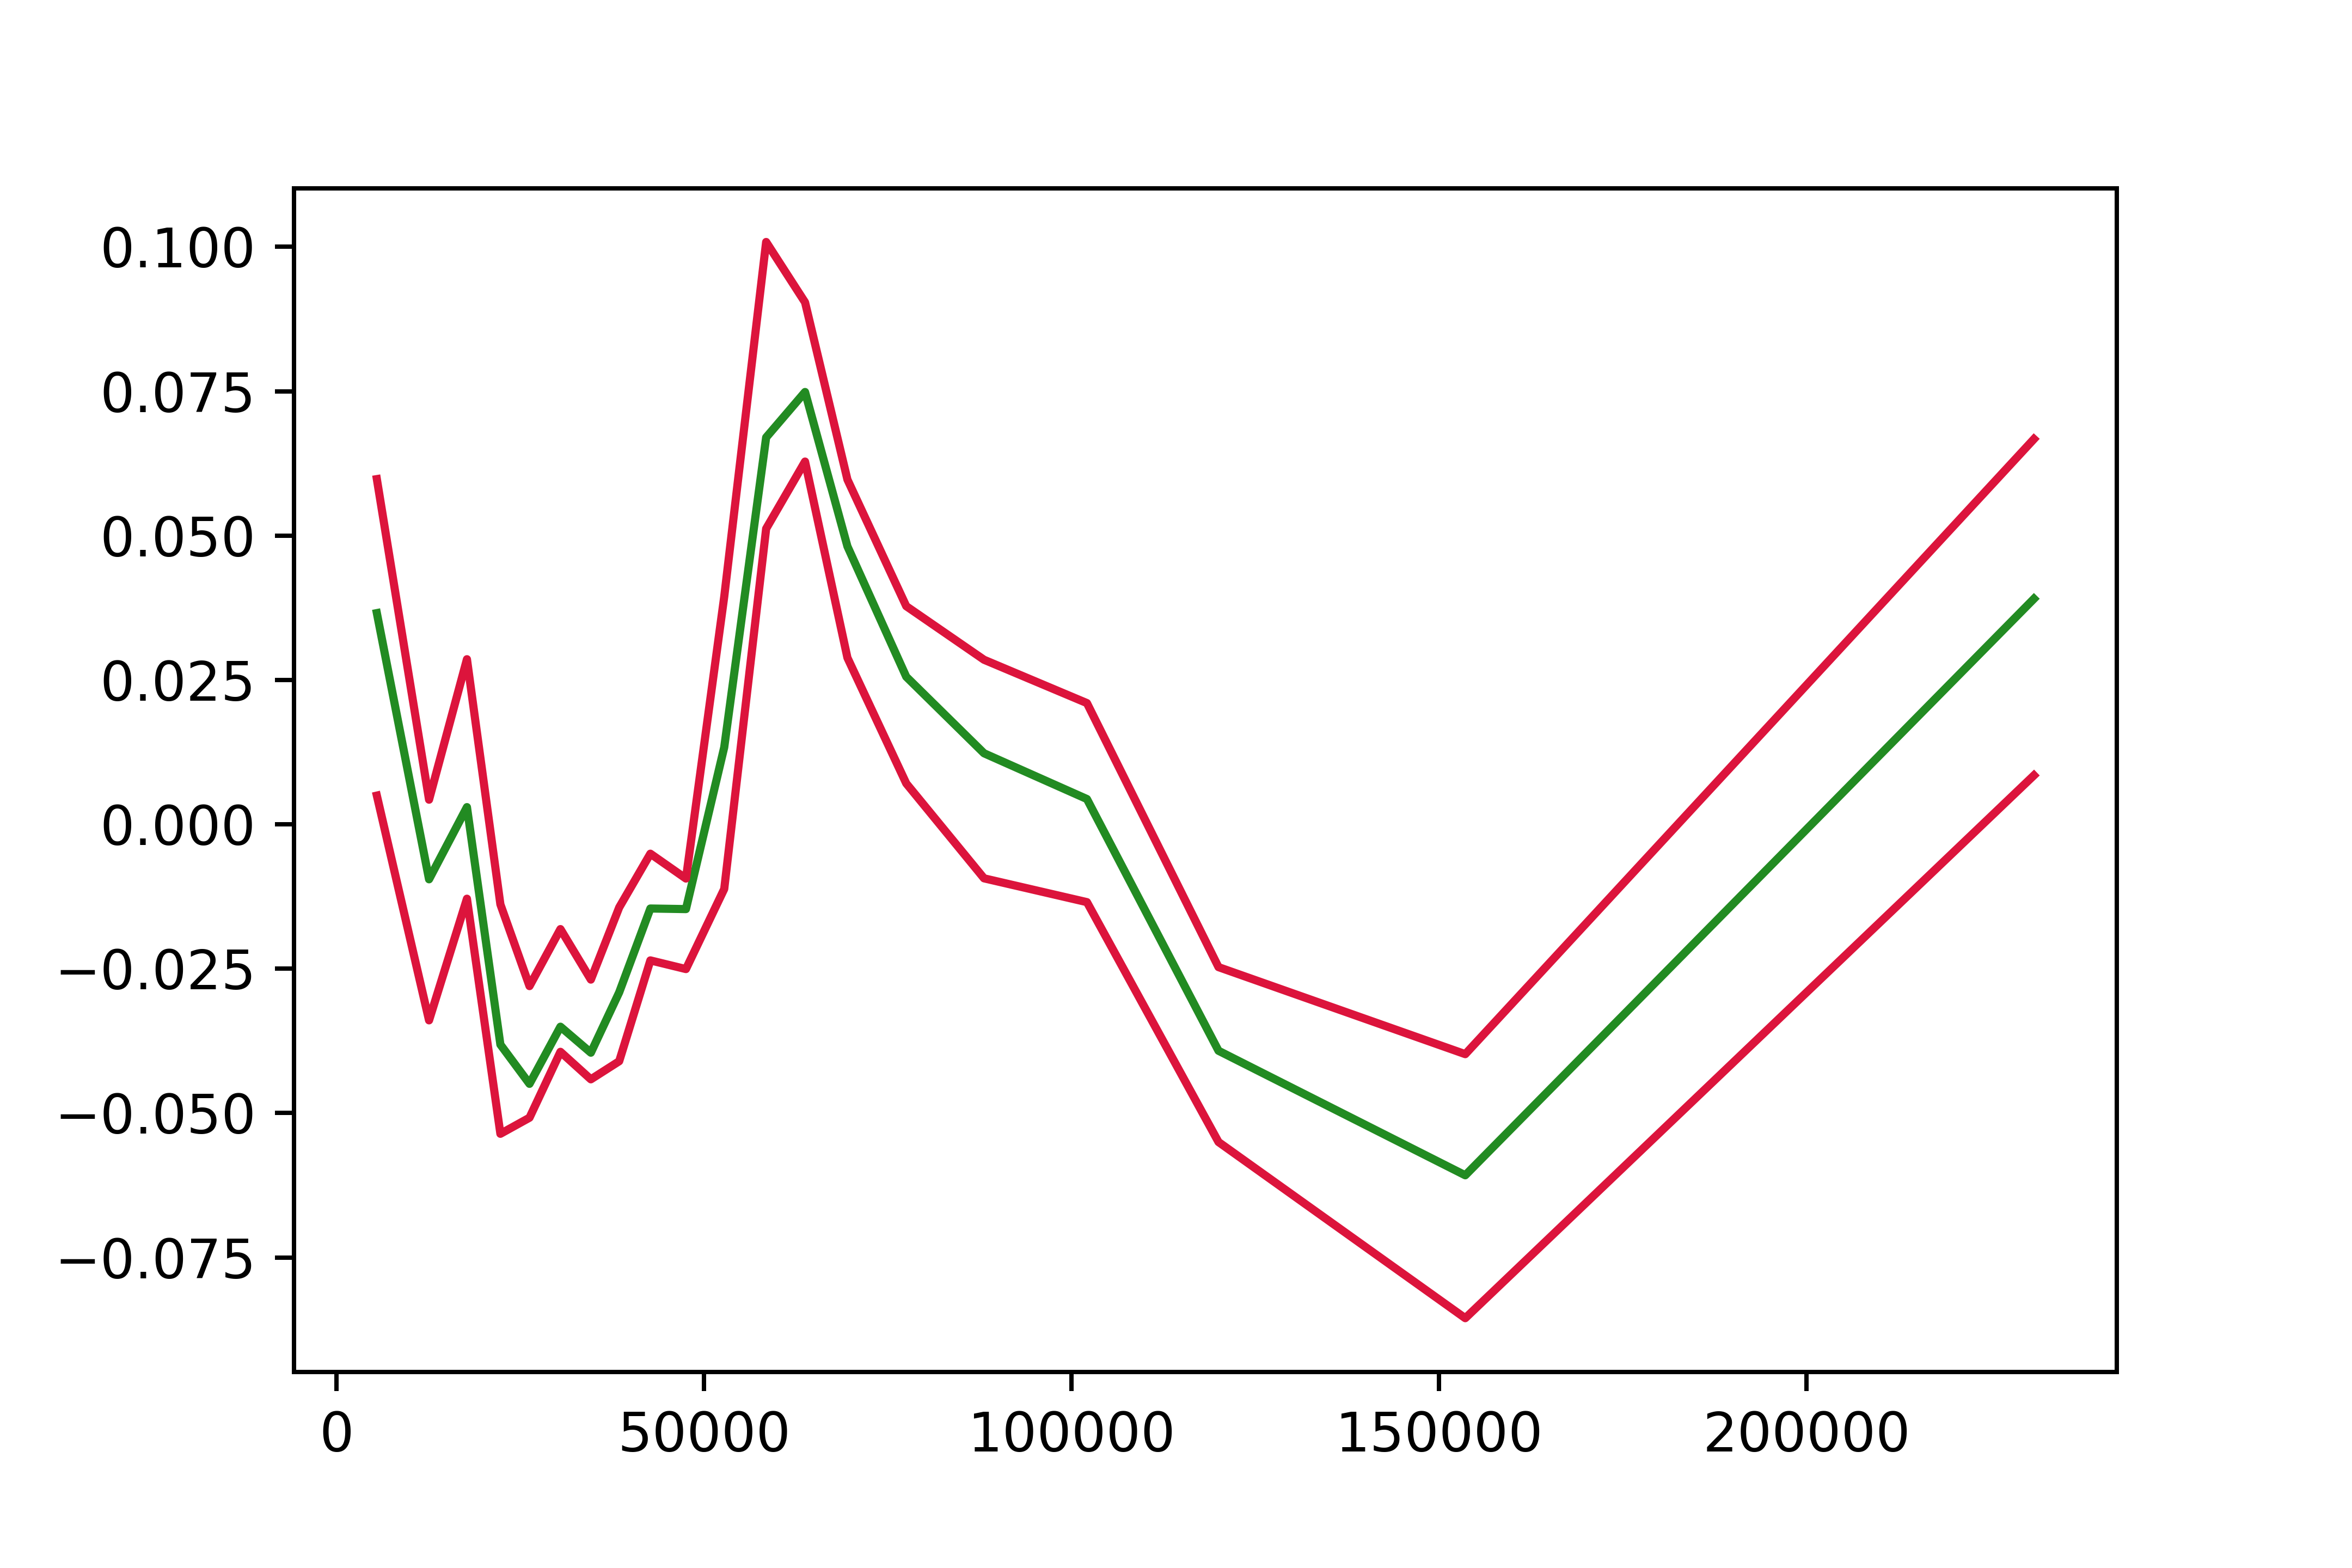
\includegraphics[width=\linewidth]{figures/ALE/chFDexp/spec3_cf_FINCBTXM.png}
        \caption{Income - causal forest}
    \end{subfigure}
    \caption{ALE of \textit{financial status} variables - total expenditures}
    \label{app:ale_finstat_fd}
\end{figure}